%  ========================================================================
%  Copyright (c) 1985 The University of Washington
%
%  Licensed under the Apache License, Version 2.0 (the "License");
%  you may not use this file except in compliance with the License.
%  You may obtain a copy of the License at
%
%      http://www.apache.org/licenses/LICENSE-2.0
%
%  Unless required by applicable law or agreed to in writing, software
%  distributed under the License is distributed on an "AS IS" BASIS,
%  WITHOUT WARRANTIES OR CONDITIONS OF ANY KIND, either express or implied.
%  See the License for the specific language governing permissions and
%  limitations under the License.
%  ========================================================================
%

% Documentation for University of Washington thesis LaTeX document class
% by Jim Fox
% fox@washington.edu
%
%    Revised 2020/02/24, added \caption()[]{} option.  No ToC.
%
%    Revised for version 2015/03/03 of uwthesis.cls
%    Revised, 2016/11/22, for cleanup of sample copyright and title pages
%
%    This document is contained in a single file ONLY because
%    I wanted to be able to distribute it easily.  A real thesis ought
%    to be contained on many files (e.g., one for each chapter, at least).
%
%    To help you identify the files and sections in this large file
%    I use the string '==========' to identify new files.
%
%    To help you ignore the unusual things I do with this sample document
%    I try to use the notation
%       
%    % --- sample stuff only -----
%    special stuff for my document, but you don't need it in your thesis
%    % --- end-of-sample-stuff ---


%    Printed in twoside style now that that's allowed
%
 
\documentclass[11pt, proquest]{uwthesis}[2020/02/24]
 
%
% The following line would print the thesis in a postscript font 

% \usepackage{natbib}
% \def\bibpreamble{\protect\addcontentsline{toc}{chapter}{Bibliography}}

\setcounter{tocdepth}{1}  % Print the chapter and sections to the toc
 

% ==========   Local defs and mods
%

% --- sample stuff only -----
% These format the sample code in this document

\usepackage{alltt}  % 
%\usepackage[version=4]{mhchem}
\usepackage{chemformula}
\let\ce\ch
\usepackage{xcolor}
\usepackage{graphicx}
\usepackage{booktabs}
\usepackage{caption}
\usepackage{subcaption}
\usepackage{float}
\usepackage{amsmath}
\usepackage{setspace}
\usepackage{graphics}
\usepackage{adjustbox}

\usepackage{textcomp}
\newcommand{\textapprox}{\raisebox{0.5ex}{\texttildelow}}

\usepackage{epstopdf}
\epstopdfDeclareGraphicsRule{.tif}{png}{.png}{convert #1 \OutputFile}
\AppendGraphicsExtensions{.tif}

\usepackage[backend=biber,style=chem-acs]{biblatex} % use autocite
\newenvironment{demo}
  {\begin{alltt}\leftskip3em
     \def\\{\ttfamily\char`\\}%
     \def\{{\ttfamily\char`\{}%
     \def\}{\ttfamily\char`\}}}
  {\end{alltt}}
 
% metafont font.  If logo not available, use the second form
%
% \font\mffont=logosl10 scaled\magstep1
\let\mffont=\sf
% --- end-of-sample-stuff ---
 
\addbibresource{all_references.bib}

\begin{document}
 
% ==========   Preliminary pages
%
% ( revised 2012 for electronic submission )
%

\prelimpages
 
%
% ----- copyright and title pages
%
\Title{The Many-Body Expansion: A powerful tool for analyzing intermolecular interactions and driving molecular dynamics}
\Author{Joseph P. Heindel}
\Year{2022}
\Program{Department of Chemistry}

\Chair{Dr. Sotiris S. Xantheas}{}{}
\Signature{Dr. Anne B. McCoy}
\Signature{Dr. Charles T. Campbell}
\Signature{Dr. Stephanie Valleau}

\copyrightpage

\titlepage

 
%
% ----- signature and quoteslip are gone
%

%
% ----- abstract
%


\setcounter{page}{-1}
\abstract{
\par The many-body expansion (MBE) is a method of decomposing any molecular property into contributions from the sub-systems of some total system. We focus on applying the MBE to detailed studies of the energy and forces of molecular clusters. In particular, we carry out the MBE up to full order for \ce{(H2O)7} and \ce{(H2O)_{10}} with increasingly complete basis sets. In doing this, we determine that the convergence of higher-order terms in the MBE depends sensitively on the presence of basis set superposition error (BSSE). Namely, the MBE for 3-body and higher terms in the energy is converged with an aug-cc-pVDZ basis set as long as a BSSE correction is included. If BSSE is ignored, however, the MBE oscillates from term to term and converges very slowly.

\par We carry out a similar analysis of ion-water clusters, \ce{Z^{+/-}(H2O)_{9}}, where \ce{Z^{+/-}}= \ce{Li^+}, \ce{Na^+}, \ce{K^+}, \ce{Rb^+}, \ce{Cs^+}, \ce{F^-}, \ce{Cl^-}, \ce{Br^-}, and \ce{I^-}. We verify the same conclusions about convergence of the MBE as for pure water clusters. Additionally, we find a remarkable linear anti-correlation between the total 2-body ion-water and 2-body and 3-body water-water interactions. This provides a quantitative measure of the extent to which hydrogen bond networks are disrupted by the presence of monoatomic ions. For both neutral and ion-water clusters, we find that the correlation energy makes less than 0.1\% total contribution to the energy at the 3-body and higher levels. That is, electron correlation only needs to be included at the 1- and 2-body levels to capture 99.9\% of the energy.

\par Additionally, we use the MBE as a tool for analyzing molecular interactions in clathrate cages of varying sizes: \ce{(H2O)_{20}}, \ce{(H2O)_{24}}, and \ce{(H2O)_{28}}. These systems are dominated by subtle cooperative hydrogen bonding effects. That is, for \ce{(H2O)_{20}} there are 30,026 unique configurations with the least stable of these lying \textapprox30 kcal/mol higher in energy than the most stable one. We show that many of the possible hydrogen bond configurations of these cages are actually not stable local minima, but instead collapse to lower energy families of networks. We use the MBE to understand how many-body effects contribute to the stability of these clathrates cages. It turns out, for these systems, that the 2- and 3-body energies decrease at nearly identical rates as the total energy increases. This means these systems are particularly sensitive to hydrogen bond cooperativity because the 3-body energy is a smaller component of the total energy than the 2-body part. This work provides a good illustration of how the MBE can be used to tease apart complex details of molecular interactions with relative ease.

\par These detailed analyses lay the groundwork for a scheme in which high levels of electronic structure theory, such as MP2 and CCSD(T), can be used to drive the molecular dynamics of medium-sized systems without a major loss of accuracy. We first demonstrate that one can use the MBE to drive dynamics simulations with the MB-Pol water potential. These simulations result in the observation that the MBE is fairly slow to converge the forces and, in certain circumstances, a 5-body description of the force may be needed. We discuss the extension of MBE-MD to \textit{ab initio} molecular dynamics simulations, emphasizing the algorithmic and software improvements which could be used to make \textit{ab initio} MBE-MD a practical method.
}
 
%
% ----- contents & etc.
%
\tableofcontents
\listoffigures
\listoftables
 
%
% ----- glossary 
%
%\chapter*{Glossary}      % starred form omits the `chapter x'
%\addcontentsline{toc}{chapter}{Glossary}
%\thispagestyle{plain}
 
%
% ----- acknowledgments
%
\acknowledgments{
  Thank you to Daniel Schofield for introducing me to computational chemistry. You prepared me excellently for graduate school. Perhaps more importantly, you showed me that humility and scientific excellence are not mutually exclusive.
  
  Thank you to Anne McCoy for letting me hang around your group. I learned many things about science and being a scientist that I would not have figured out otherwise. You were also excellent at keeping my ego in check, which, on its own, is uncontrollably self-inflating.
  
  Finally, thank you to my advisor, Sotiris Xantheas. You have treated me like family and I appreciate that immensely. You have given me every opportunity to succeed in science. I hope I can make something of these favorable initial conditions.
  }

%
% ----- dedication
%
%\dedication{\begin{center}??\end{center}}

%
% end of the preliminary pages
 
 
 
%
% ==========      Text pages
%

\textpages

\chapter{Simulating Properties of Molecular Systems}

Observing the behavior of the physical world can be both an illuminating and deeply confusing activity. There is a dizzying array of complexity surrounding us all the time, both in the form of natural phenomena and technologies created by humans that exploit those natural phenomena. In this work, we will be concerned with how to make sense of this complexity. There are many possible approaches to understanding nature, but we will focus on just the one that this author prefers. Namely, we will describe various ways of simulating physical systems and thereby attempt to understand their behavior by reproducing it on a computer.
%\footnote{Observing the behavior of humans almost exclusively amplifies this confusion, so I will ignore them for the rest of this thesis.}

\section{Macroscopic Properties and Ensembles}

If we are interested in understanding the world around us, then we should start by describing the properties of a system we find intriguing. These are things like color, phases of matter, viscosity, electrical conductivity, compressibility, and so on. We will refer to these aspects of bulk materials as macroscopic properties. As it happens, all bulk materials are made up of smaller components in the form of molecules (or just lattices of atoms for many solids). When one zooms in on a material and thinks of it as a large collection of molecules, the connection of these molecules to some macroscopic property can be difficult to see. Making the connection between a macroscopic property and a collection of molecules is the purview of statistical mechanics.\autocite{tuckerman_statistical_2010}

\par In order to avoid summarizing the entire field of statistical mechanics, which is vast, we will skip to the point and say that macroscopic properties can be calculated by sampling the partition function of a statistical ensemble. Briefly, an ensemble is the distribution of states that a system can occupy. The partition function is a mathematical object that relates microstates (collections of atoms and molecules in a particular configuration) to macroscopic properties. There are many types of ensembles, but we will focus on thermodynamic ensembles, which describe systems in equilibrium and hence obey certain constraints such as a fixed temperature and volume. For every thermodynamic ensemble, there is an associated partition function which depends on all of the possible microstates of a system. If we can sample these microstates and either exactly or approximately calculate the partition function, then we can make the desired connection between collections of molecules and macroscopic properties.

\par Before we discuss methods of sampling partition functions, let us look at the form of a partition function to get a better feel for the problem. Consider the partition function associated with the canonical ensemble, which has a fixed number of particles, volume, and temperature. The partition function, $Z$, takes the form,
\begin{equation}
    Z=\sum_ie^{-\beta E_i}
    \label{eq:z_discrete}
\end{equation}
where $\beta=1/k_bT$ with $k_b$ Boltzmann's constant and $T$ the thermodynamic temperature. The sum in Eq. \ref{eq:z_discrete} runs over all possible microstates of the system with associated energy $E_i$. Clearly, calculating this quantity is very difficult in general because the energy might be a complicated function of the configuration of particles and there may be infinitely many states to sum over. Indeed, in the case that energies are continuous, which is often a very good approximation in condensed phases, the partition function is written as,
\begin{equation}
    Z=\frac{1}{h^{3N}N!}\int \exp\left(-\beta \sum_i H(\mathbf{q}_i,\mathbf{p}_i)\right)d^3\mathbf{q}d^3\mathbf{p}
    \label{eq:z_continuous}
\end{equation}

In the continuous case of Eq. \ref{eq:z_continuous}, the sum turns into an integral and the energy is represented by the Hamiltonian of the system, $H(\mathbf{q},\mathbf{p})$. I have used bold face to indicate the positions, $\mathbf{q}$, and momenta, $\mathbf{p}$, are 3-dimensional vectors. $N$ is the number of atoms in the system and $h$ is Planck's constant.

Let us go one step further to highlight the most important property of the partition function for our purposes. The Hamiltonian is given by
\begin{equation}
    H=\sum_{i=1}^N\frac{\mathbf{p}_i^2}{2m_i}+V(\mathbf{q})
    \label{eq:hamiltonian}
\end{equation}
where $V(\mathbf{q})$ is a potential energy function which depends on all atomic positions $\mathbf{q}$. Since the momentum is quadratic, it is easy to show that the momentum can be analytically integrated out of the partition function in Eq. \ref{eq:z_continuous}. If we do this, we are left with the following expression,
\begin{equation}
    Z=\frac{1}{N!}\left(\frac{2\pi m}{\beta h^2}\right)^{3N/2}\int \exp\left(-\beta V(\mathbf{q})\right)d^3\mathbf{q}
    \label{eq:configuration}
\end{equation}
Now we see that Eq. \ref{eq:configuration} has a pre-factor which depends on the masses of each atom and the temperature (I have written it assuming a single mass for all atoms). So, essentially all of the physics that the partition function encodes is contained in the integral piece of Eq. \ref{eq:configuration}. This integral is called the configuration integral because it is an integral over all possible configurations of the atoms, where each configuration contributes a value equal to $\exp\left(-\beta V(\mathbf{q})\right)$. This is an important result as it says that the function describing the local interactions between molecules, $V(\mathbf{q})$, contains all the information necessary to describe macroscopic material properties.

\par Therefore, the configuration integral gives us an entry point to simulate macroscopic properties using configurations of molecules. There are two questions we need to answer in order to solve the configuration integral. First, since the integral is over all configurations of all atoms in space, how do we sample these infinitely many configurations? Second, how do we construct and calculate the potential energy function $V(\mathbf{q})$? We will start by discussing two techniques for sampling the configurations needed to calculate the configuration integral: (i) monte carlo and (ii) molecular dynamics. Then we will turn our attention to methods of constructing and calculating the potential energy function, $V(\mathbf{q})$, where we will see this is the centrally difficult problem in statistical mechanical simulations.

\section{Sampling Configurations with Monte Carlo}

One well known and general strategy for numerically solving integrals is the monte carlo (MC) method. We can randomly sample configurations and evaluate the potential energy at these configurations to solve the configuration integral in Eq. \ref{eq:configuration}. The problem is that the random samples we take should not be uniformly distributed, but should be sampled with a frequency proportional to the integrand, $\exp(-\beta V(\mathbf{q}))$. The most common and well-known technique for generating samples that obey this distribution is the Metroplis-Hastings algorithm.\autocite{metropolis_monte_1949}

\par The Metroplis-Hastings algorithm has been described in detail in many places, so we will focus on the details which are most pertinent to the research contained in this thesis.\autocite{chib_understanding_1995} The most important steps in the algorithm are (i) generating proposed configurations and (ii) evaluating the potential energy at this configuration. The former step is entirely arbitrary and many types of moves can be designed and tailored to the specific system being studied. The proposed configurations will then be accepted or rejected according to the Metropolis condition which, for the canonical ensemble, can be stated concisely as,
\begin{equation}
    \min\left(1,\frac{\exp(-\beta V(\mathbf{q}_{proposed}))}{\exp(-\beta V(\mathbf{q}_t))}\right)
    \label{eq:metropolis}
\end{equation}
where $\mathbf{q}_{proposed}$ is the proposed configuration and $\mathbf{q}_{t}$ is the configuration from step $t$ of the simulation. That is, we will accept the proposed configuration when the second argument in Eq. \ref{eq:metropolis} is smaller than one. The centrality of the potential energy function, $V(\mathbf{q})$, in MC simulations should now be evident. Indeed, while there is something of an art-form associated with proposing candidate configurations, the actual distribution of configurations is determined entirely by the potential energy function.

\par At this point I would like to point out two drawbacks of MC sampling of the configuration integral. The first is that, by design, the Metropolis-Hastings algorithm rejects many proposed configurations. This means that the potential energy must be evaluated on many configurations which do not end up contributing to our approximation of the partition function. These calculations amount to wasted computer time. The second drawback is more severe but requires a bit of a tangent to explain completely.

\par If we can successfully compute the configuration integral, then we can also successfully calculate any average quantity over the ensemble of interest. In the case that the average quantity of interest depends only on the position, the ensemble average, $\langle G(\mathbf{q})\rangle$, takes the form,
\begin{equation}
    \langle G(\mathbf{q})\rangle=Z^{-1}\int \exp\left(-\beta V(\mathbf{q})\right)G(\mathbf{q})d^3\mathbf{q}
    \label{eq:average}
\end{equation}
Eq. \ref{eq:average} says that the ensemble average of any quantity is the configurationally averaged value of that same quantity normalized by the partition function. Solving this integral is no different than solving the plain configuration integral discussed above.

\par This is an excellent result if the only properties of interest are ensemble averaged properties. Very often, however, one might care about dynamic properties of a system such as various time correlation functions which are related to things like the infrared spectrum and diffusion constant. These quantities are very hard to calculate from a MC sampling of the configuration integral because successive configurations are not ordered in time. Indeed, there is no straightforward definition of time in a MC simulation. Therefore, if we are interested in dynamic properties of a system, we should turn our attention elsewhere.

\section{Sampling Configurations with Molecular Dynamics}
The other approach for sampling molecular configurations is through molecular dynamics (MD) simulations. Let us first discuss the fundamentals of MD and then we will describe why one would choose MD simulations over MC. To put it simply, MD samples molecular configurations by trying to mimic the dynamics of a molecular system by assuming they obey Newton's equations of motion. The algorithm for MD is fairly straightforward as long as we have a differentiable potential energy function, $V(\mathbf{q})$. In short, we integrate Newton's equations using something like Verlet integration\autocite{verlet_computer_1967}, which allows us to propagate a set of molecular configurations forward in time. Verlet integration generates a configuration for atom $i$ at time $\Delta t$ into the future, $\mathbf{q}_i(t+\Delta t)$, from the current configuration $\mathbf{q}_i(t)$ as follows,
\begin{equation}
    \mathbf{q}_i(t+\Delta t)=2\mathbf{q}_i(t) - \mathbf{q}_i(t-\Delta t) -\frac{\nabla_i V(\mathbf{q})}{m_i}\Delta t^2
    \label{eq:verlet}
\end{equation}

Eq. \ref{eq:configuration} showed that we only need to calculate the energies of molecular configurations to sample an ensemble, so it is fair to wonder why MD would ever be preferable to MC when it requires calculating the gradient of the potential energy, $\nabla_i V(\mathbf{q})$, which is slower than just evaluating the potential energy.

There are two main advantages of MD over MC which I would like to highlight. The first is that MD simulations sample configuration space very efficiently by trying to mimic the actual nuclear dynamics of a system. So, even though calculating gradients of a potential can be slow, this cost is typically offset by efficiently generating configurations relevant to the sampling of an ensemble. The second is that MD allows for the calculation of dynamic properties of a system such as the infrared spectrum from the dipole auto-correlation function or the diffusion coefficient from an integral over the velocity auto-correlation function.\autocite{green_markoff_1954}

It is important to note that different observables require different simulation lengths to be calculated accurately. For instance, calculating the infrared spectrum of liquid water requires simulations on the order of several tens of picoseconds, which is quite short, because this is roughly the decorrelation time of dipoles in the system. The exact timescale depends on temperature, but this is an example of a rather easy-to-evaluate observable. Compare this with the calculation of the dielectric constant of a solvent which typically requires tens of nanoseconds of simulation time.\autocite{gereben_accurate_2011} While MD provides access to dynamical observables and efficiently samples configuration space, the actual observables one can calculate will depend on the length of simulation one can afford to propagate. The maximum accessible simulation time will always be determined by the computational complexity of the chosen potential energy function.

\section{Path Integral Molecular Dynamics}
One major assumption of the MC and MD formulations we just introduced is that the nuclei can be represented as point-particles. That is, we ignored the quantum nature of the nuclei and hence these simulations do not account for zero point energy, which can be a bad approximation for systems that depend sensitively on the motion of hydrogen atoms.\autocite{markland_nuclear_2018} Additionally, at very low temperatures even heavier atoms like oxygen exhibit large quantum delocalizations, meaning classical MD is unlikely to be a good approximation of the nuclear dynamics.\autocite{schran_converged_2018,schran_quantum_2019} Fortunately, there is a relatively simple form of both MC and MD which can be derived from the path integral formulation of quantum mechanics.\autocite{feynman_quantum_2010}

\par Beginning from the quantum density matrix, an expression for the quantum partition function can be derived which can then be sampled via path integral molecular dynamics (PIMD). The Hamiltonian governing the dynamics of the system can be shown to be\autocite{chandler_exploiting_1981},
\begin{equation}
    H_P(\mathbf{p}, \mathbf{q})=\sum_{i=1}^N\sum_{k=1}^P\left(\frac{|\mathbf{p}_i^{(k)}|^2}{2m_i}+\frac12m_i\omega_k^2|\mathbf{q}_i^{(k)}-\mathbf{q}_i^{(k-1)}|^2\right) + \sum_{k=1}^PV(\mathbf{q}_1^{(k)},\cdots,\mathbf{q}_N^{(k)})
    \label{eq:rp_hamiltonian}
\end{equation}

The Hamiltonian in Eq. \ref{eq:rp_hamiltonian} is basically the same as the ordinary $N$-atom Hamiltonian in Eq. \ref{eq:hamiltonian} except it contains an extra sum over the index $k$. Therefore, this Hamiltonian governs the dynamics of $P$ replicas of $N$ atoms, rather than just the $N$ atoms we would normally have in classical dynamics. Also, our sampling of the quantum partition function becomes exact as $P\rightarrow\infty$. Eq. \ref{eq:rp_hamiltonian} also contains an extra kinetic term which harmonically couples each replica of the system in a circular manner (i.e. $\mathbf{q}_i^{(1)}$ connects to both $\mathbf{q}_i^{(N)}$ and $\mathbf{q}_i^{(2)}$) with a harmonic frequency $\omega_k=P/\beta\hbar$. Because of the extra harmonic term, this Hamiltonian is typically called the ring polymer hamiltonian and the associated dynamics technique is called ring polymer molecular dynamics (RPMD).

RPMD is a powerful method because by propagating $P$ replicas of a classical system, we are able to collect ensemble averages which account for nuclear quantum effects. While this is quite effective, it can also be very expensive due to the fact we now have to evaluate energies and forces for $P$ copies of the system, where $P$ typically ranges from around 30 up to several thousand depending on the temperature and system of interest. Therefore, just like with ordinary MD, the ability to utilize PIMD is limited by the cost of evaluating energies and forces from the chosen potential energy function. With this in mind, let us finally turn our attention to molecular potential energy functions and discuss them in detail.

\section{Potential Energy Functions}
We will break our discussion of methods for evaluating molecular potential energies and forces into two classes. The first consists of classical approximations of molecular interactions which we will call force fields. The second consists of approximations to the electronic Schrodinger equation which results in a so-called \textit{ab initio} potential energy surface (PES). We will describe the pros and cons of each approach and then focus on how we can bridge the gap between these methods, which forms the main subject of this thesis.
\subsection{Molecular Mechanics Force Fields}
The simplest approach to generating forces for MD consists of using analytic equations for the intra- and intermolecular degrees of freedom, typically called molecular mechanics (MM). Some examples of possible interaction terms in MM force fields are Lennard-Jones terms\autocite{jones_determination_1924,jones_determination_1924-1}, Morse potentials\autocite{morse_diatomic_1929}, Buckingham exponentials\autocite{buckingham_classical_1938}, or suitably modified versions of these\autocite{werhahn_new_2015}. Additionally, a coulomb term is typically employed to account for the electrostatic interactions. Bonded interactions typically take the form of harmonic bond and angle terms with a cosine potential for dihedral interactions. In this sense, MM force fields can be viewed as advanced ball-on-a-spring models.

\par Evaluating MM force fields is extremely fast because the intermolecular part is pairwise additive and the intramolecular part consists of very simple functions. The fact that these interactions are pairwise additive is clearly incorrect. The electronic distribution of a molecule is affected by the presence of other molecules in a non-additive manner\autocite{stone_theory_2013}. In the simplest case, one can be certain that the charge on a particular atom in a molecule (which is not even well-defined in quantum mechanics) will change its value in the presence of other charges. In other words, MM force fields completely neglect atomic and molecular polarizabilites. In order to compensate for this and many other errors inherent to these simplified potentials, one must carefully parameterize each term to reproduce some experimental property.

\par Because of their heuristic nature, MM force fields rely on large cancellations of errors in the potential with the further hope that errors in the short-time dynamics will be averaged out to provide approximately correct long-time dynamics. Indeed, MM tries to parameterize the complexities of quantum mechanics into simple functions so that very large ensembles can be thoroughly sampled. Not only that, but MM force fields are often parameterized to reproduce experimental data, which means the parameters bake in effects like zero point energy and target a certain region of the phase diagram. This parameterization strategy means that MM force fields are not suitable for PIMD simulations because one would effectively overcount zero point energy.

\par Despite these limitations, for many systems such as large biological molecules, MM is the only feasible approach. That is, there are many physical systems which are large and spatially heterogeneous, which means one must use easy-to-evaluate force fields to adequately sample the associated ensemble. If, on the other hand, one is interested in intricate details of a system's dynamics, especially those influenced by quantum mechanical effects, then MM is entirely useless because it avoids these complexities by design. We will first look at a class of force fields which aims to reproduce quantum mechanical interactions and then look at the feasibility of utilizing explicit approximations to the Schrodinger equation in MD.
\subsection{Advanced Force Fields}
\par We just learned that MM force fields are sometimes very inaccurate and are not suitable for nuclear quantum simulations, which limits the types of systems and macroscopic properties one can reliably study. We will now look at advanced force fields, which aim to reproduce the electronic energy of a system without actually using quantum mechanics. Advanced force fields do this primarily by introducing polarizabilities to each atom which allows a force field to be transferable across environments. Additionally, introducing polarization allows these force fields to better describe short-range electronic interactions, which MM almost universally fails to describe with any fidelity. I will focus specifically on potentials attempting to model the interactions between water molecules although there are similar potentials for other important systems.

\par Some of the earliest advanced force fields are those which model many-body effects by using polarizable atoms. There is a well-known short-range singularity when polarizable atoms interact which can be circumvented using damped interactions as introduced by Thole\autocite{thole_molecular_1981}. When using Thole damping, the dipole ineraction tensor is modified in such a way that the short range singularity becomes physically inaccessible (although it still exists in principle, just at distances too short to sample in any reasonable simulation). This modification of the dipole interaction tensor takes the following form\autocite{thole_molecular_1981},
\begin{equation}
    T_{ij}=\frac{f_e}{r_{ij}}\mathbf{I}-\frac{3f_t}{r_{ij}^5}
    \begin{bmatrix}
    x^2 & xy & xz \\
    yx & y^2 & yz \\
    zx & zy & z^2 \\
    \end{bmatrix}
    \label{eq:thole_damping}
\end{equation}

The modified dipole tensor in Eq. \ref{eq:thole_damping} is the same as the normal dipole tensor, which only depends on the distance between two polarizable sites, $r_{ij}$, except it contains two damping functions, $f_e$ and $f_t$. Thole proposed both linear and exponential forms of these damping functions, though the choice of damping function is arbitrary and hence can be viewed as a parameter in the model. Typically, however, the exponential form proposed by Thole is used. This dipole interaction tensor must be formed for all polarizable sites, then the induced dipolar interaction energy is calculated according to the Applequist model.\autocite{applequist_atom_1972}

\par The Thole-type water models (TTM) use a simple parameterization based on MP2/CBS calculations of the \ce{(H2O)2} PES to generate quite accurate water models\autocite{burnham_development_2002,burnham_development_2002-1,fanourgakis_flexible_2006,fanourgakis_development_2008}. The non-linearity of the dipole moment surface in TTM models resulted in the first water models to correctly capture the opening of the bend angle in water going from the gas phase to condensed phases\autocite{fanourgakis_bend_2006}.

\par Another approach to developing accurate, advanced force fields was popularized by Joel Bowman in the form of permutationally invariant polynomials (PIPs)\autocite{braams_permutationally_2009}. This technique allows for relatively high-dimensional functions to be explicitly fit as long as sufficient data is available. Even more importantly, PIPs respect the relevant physical symmetries in that the energy is translationally, rotationally, and permutationally invariant (that is, swapping identical atom types does not change the energy). This innovation in function-fitting was cleverly combined with the many-body expansion, a technique we will discuss in detail in the next section, to produce extremely accurate models. The earliest of these models are the HBB2\autocite{huang_ab_2006} and WHBB\autocite{wang_full-dimensional_2009} models. These same techniques were used by the group of Francesco Paesani to create the MB-Pol water model\autocite{babin_toward_2012, babin_development_2013, babin_development_2013-1, babin_development_2014}. It is worth mentioning that a recent model, MB-UCB\autocite{das_development_2019}, has been released which, in the spirit of TTM, avoids the heavy parameterization of PIP-based models while achieving accuracy comparable to MB-Pol.

\par Advanced force fields have been very important in the study of water and many other systems. At this point, the theoretical chemistry community is very proficient at developing these force fields with a variety of different approaches. While excellent progress has been made, developing advanced force fields is inherently difficult and once a model is complete there is a long process of validation against available experimental and theoretical results. Even worse, these force fields are often system-specific and it is very difficult, if not impossible, to extend the potential to include atoms other than those which the model originally included. For instance, models based on explicitly fitting terms in the many-body expansion (MBE) suffer from a combinatorial explosion of pairings of atom-types. For this reason, it is very unlikely that models based on directly fitting the MBE will ever progress beyond two-component systems and some three-component systems of special interest.

\par To summarize, MM force fields aim to be very efficient and applicable to a wide range of systems. Advanced polarizable force fields aim to be more accurate and applicable across the entire phase diagram albeit they lack the generality of the MM force fields as they are typically developed for a specific system. Furthermore, polarizable force fields try to reproduce the quantum mechanical potential energy, and hence are the only force fields for which PIMD simulations are appropriate. The drawback is that polarizable force fields can be difficult to construct and are quite more expensive than MM force fields. All force fields, however, are vastly faster than doing explicit quantum mechanical calculations. That being said, quantum mechanics provides many advantages, which force fields can never reproduce, and we will now explore.

\section{Ab initio Molecular Dynamics}
\par Generating forces for molecular dynamics through \textit{ab initio} calculations is a powerful and general approach, which has been utilized extensively since the mid-1980s. The most straightforward form of \textit{ab initio} molecular dynamics (AIMD) is to simply use the energy gradients from any electronic structure method with the same type of integrator one might use in regular MD simulations. This technique propagates the nuclei on the Born-Oppenheimer potential energy surface (PES). While Born-Oppenheimer MD (BOMD) is simple, there are very few systems for which it is useful because extremely small time steps have to be used in order to accurately integrate the electronic motions. There are some relatively recent approaches that attempt to solve this problem\autocite{kuhne_efficient_2007}, but by the far the most common technique is to instead use Car-Parrinello MD\autocite{car_unified_1985}.

\par In Car-Parrinello MD (CPMD) simulations, the system dynamics are generated from the Euler-Lagrange equations associated with an extended Lagrangian. That is, certain extra degrees of freedom, which have no concrete physical meaning, are added to the usual Lagrangian while still guaranteeing that this Lagrangian samples the same ensemble as the real system. The extra degrees of freedom in CPMD are pseudo-particles with a fictitous mass which are cleverly utilized to slow down the electronic motions. This allows much longer time steps to be used when integrating the equations of motion than in BOMD.

\par Even though CPMD solves a major problem with AIMD by coercing electronic degrees of freedom to change on the same time scale as nuclear ones, there is no escaping the fact that electronic structure calculations are often several orders of magnitude more computationally expnsive than force fields. This difference in speed is only exacerbated further as the system size increases due to the poor scaling of electronic structure methods.

\begin{figure}
    \centering
    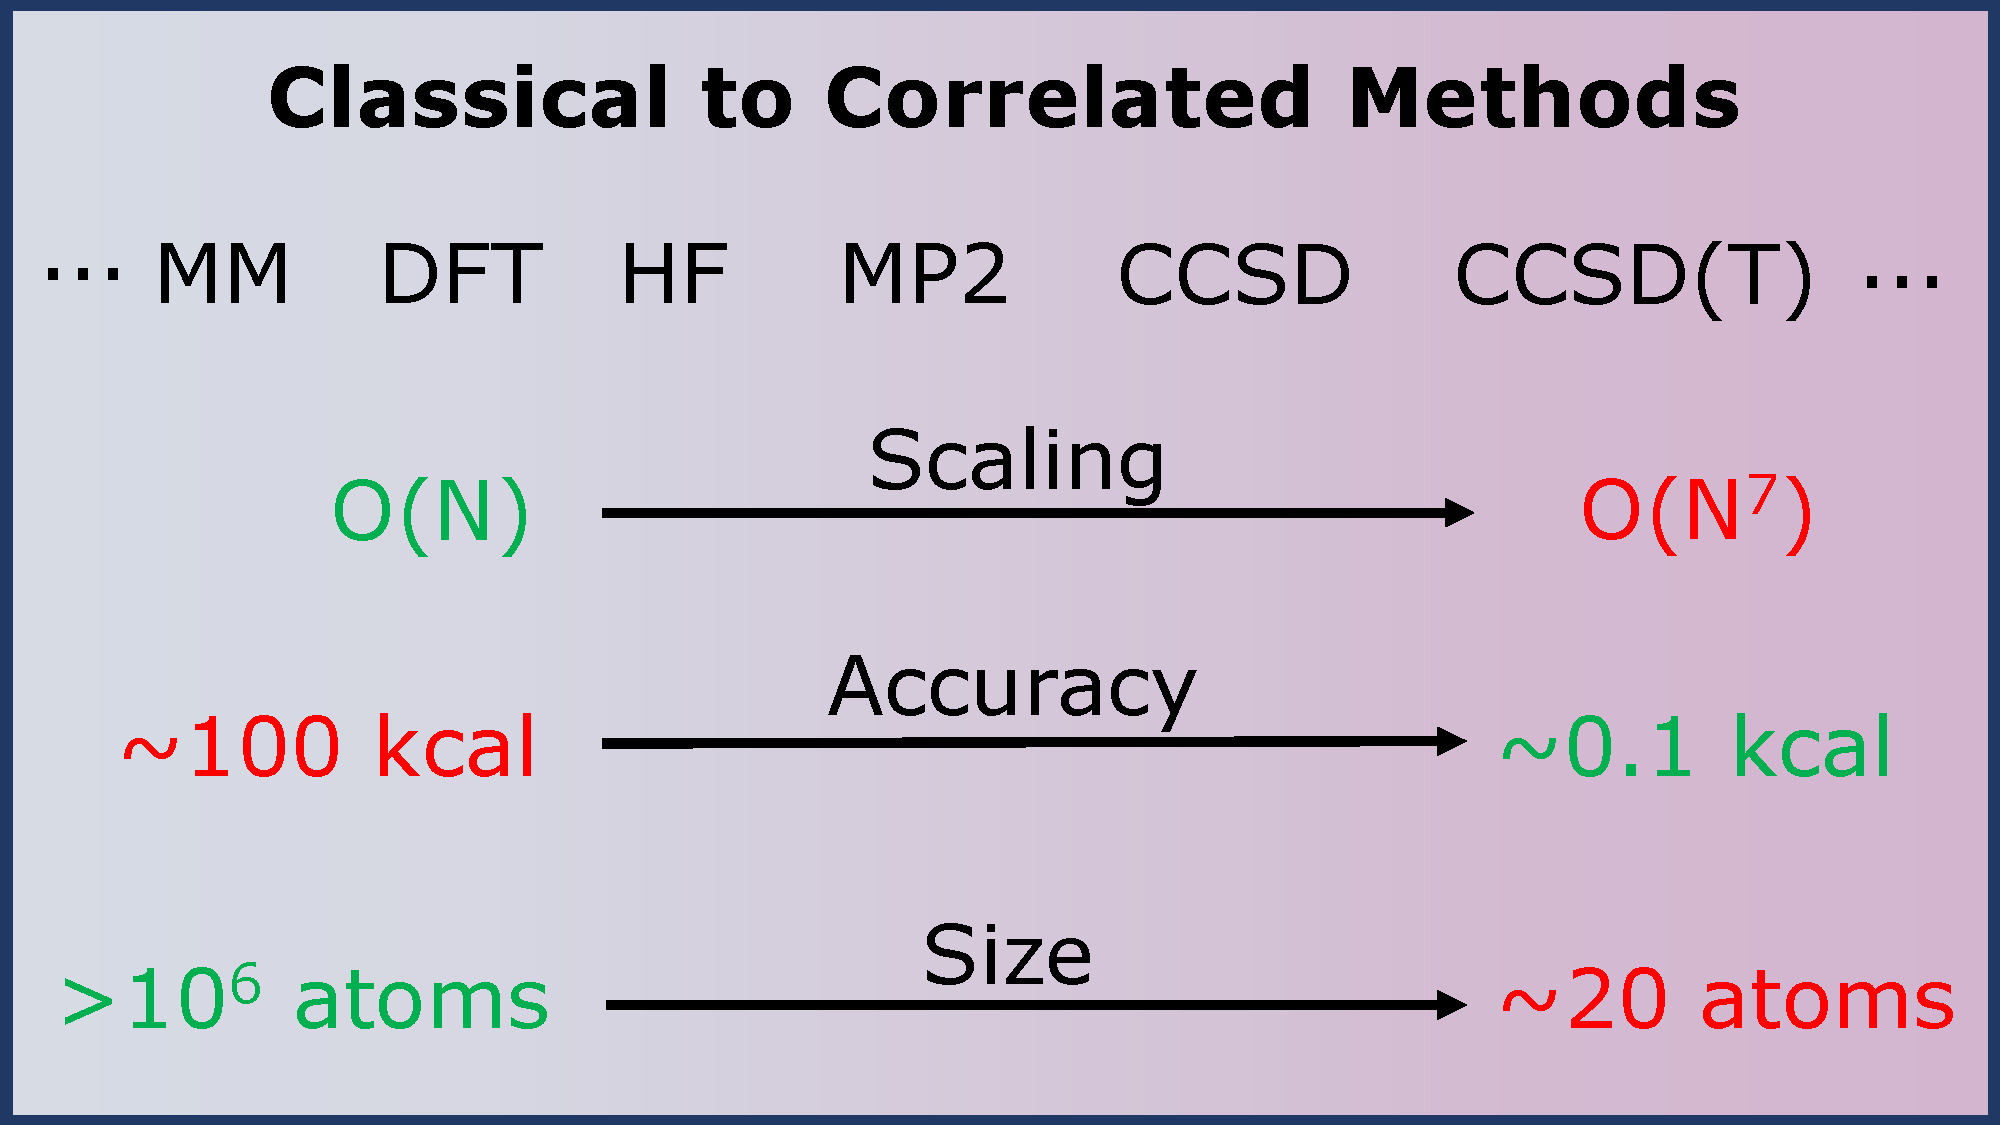
\includegraphics[width=\textwidth]{Figures/scaling_figure.pdf}
    \caption{A schematic figure showing the trade-offs as one moves from force field methods such as MM up through electronic structure methods with increasing levels of electron correlation.}
    \label{fig:es_scaling}
\end{figure}

Figure \ref{fig:es_scaling} shows the scaling of a range of popular electronic structure methods as well as the force field methods we have already discussed. Clearly, the scaling of the electronic structure methods is much worse than force field methods. Consequently, the accessible system sizes for electronic structure are much smaller than for force fields. On the other hand, electronic structure methods are typically more accurate especially when they include higher levels of electron correlation, whereas MM methods tend to provide only qualitative accuracy. In truth, Fig. \ref{fig:es_scaling} is an over-simplification because there are many force field methods which would outperform simpler electronic structure methods like Hartree-Fock (HF) and be much cheaper to evaluate. So, one really needs to include electron correlation at some level before accuracy can be expected to be uniformly better than force field methods. For this reason, CPMD mainly relies on Density Functional Theory (DFT), which is a cheaper correlated electronic structure method. Finally, electronic structure methods are transferable to any type of system and naturally allow for reactive simulations. These are huge advantages, which we would like to utilize. Therefore, we will spend the rest of this thesis exploring approaches for circumventing the poor scaling of electronic structure with the aim of making highly-correlated, \textit{ab initio} methods viable for MD simulations. We will primarily approach this by using a mathematical protocol called the many-body expansion.

\chapter{The Many-Body Expansion}

\par The many-body expansion (MBE) is an important tool first used in theoretical chemistry to quantify non-additivities in molecular interactions.\autocite{hankins_hydrogen-bond_1970} The MBE is able to do this by breaking down a system into physically meaningful fragments. These fragments might be individual molecules or sub-units of a covalently bound system (i.e. functional groups). In principle, just about any property can be written in terms of the MBE, but we will focus on the energy and forces as these are the most important properties for our purposes.

\par The binding energy of a system can be written in terms of 1-body, 2-body, 3-body, all the way to $n$-body terms, where $n$ is the number of fragments, as follows:
\begin{align}
    E_{1B} &= \sum_{i=1}^nE(i)-E_{ref,i} \\
    E_{2B} &= \sum_{i<j}E(i,j)-E(i)-E(j) \\
    E_{3B} &= \sum_{i<j<k} E(i,j,k)-E(i,j)-E(i,k)-E(j,k)+E(i)+E(j)+E(k)
\end{align}

In the above equations, $E(i)$ is the energy of the $i$th fragment in the system and $E_{ref,i}$ is a reference energy for that same fragment. Hence, $E_{1B}$ can be interpreted as a deformation energy. The total binding energy is the sum of all of the $E_{iB}$ terms. If $E_{3B}=0$, then the interactions are strictly pairwise additive, as would be the case for non-polarizable systems. This can be a good approximation for very weakly interacting systems, but for systems like water with strong, directional interactions, the 3-body component of the binding energy can be larger than 20\% of the total.\autocite{xantheas_ab_1994}

\par The MBE can be written in a more concise manner for any $k$-body term, $k<n$, by noticing that every fragment appears in a particular term the same number of times and that number is a binomial coefficient related to the order of interest, $k$, and the total number of fragments $n$. For the sake of generality, I will write this expression in terms of a 3$N$-dimensional force vector, $\mathbf{f}_N$, where $N$ is the total number of atoms. The $k+1$-body contribution to the forces, $\mathbf{f}_N^{(k+1)}$ is,
\begin{equation}
    \mathbf{f}_N^{(k+1)}=\sum_{m=0}^k(-1)^{m}\binom{N-k+m-1}{m}\sum_{n=1}^{\binom{N}{k-m+1}}\mathbf{f}_N^{(k-m+1)}.
\end{equation}

Notice that one would normally think of the $k$-body forces as being a vector of dimension $3k$. In this case, however, all force vectors $\mathbf{f}_N^{(k-m+1)}$ are $3N$-dimensional such that each atom only contributes to the indices of that atom in the total system. The forces for all other indices are filled with zeros. This expansion allows for the propagation of nuclear dynamics, as in ordinary MD, with a many-body description of the forces. There are many possible advantages to expanding forces in terms of the MBE, not the least of which is that the total system size is split into many small sub-systems, effectively circumventing the computational scaling of the method used to describe the forces.

\begin{figure}[t]
\uwsinglespace
\begin{center}
\begin{minipage}{0.4\textwidth}
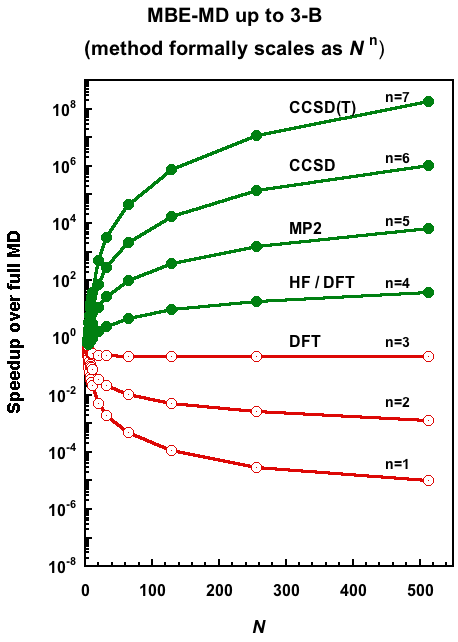
\includegraphics[width=\textwidth]{Figures/Chapter_4/ch4_figure_1_left.png}
\end{minipage}
\begin{minipage}{0.4\textwidth}
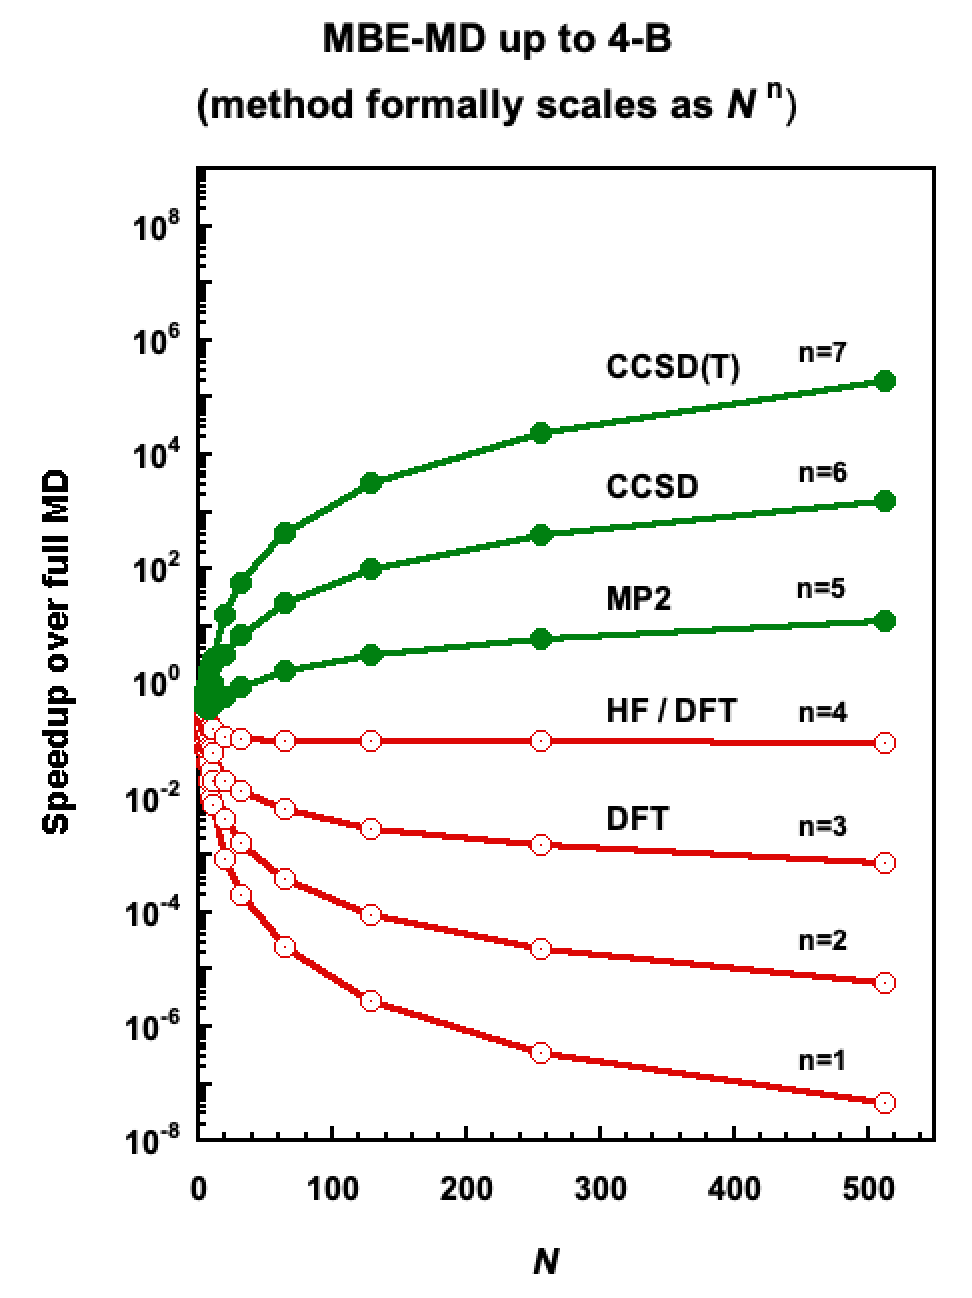
\includegraphics[width=\textwidth]{Figures/Chapter_4/ch4_figure_1_right.png}
\end{minipage}
\end{center}
\begin{spacing}{1.0}
\caption[Asymptotic speed-up of the MBE compared to a full calculation for varying numbers of fragments and various polynomial scaling of the relevant electronic structure method compared to a calculation on the full system. Each method is represented with a polynomial scaling as $N^n$, where $N$ is the number of fragments and $n$ the polynomial scaling exponent of the method in question.]{Asymptotic speed-up of the MBE compared to a full calculation for varying numbers of fragments and various polynomial scaling of the relevant electronic structure method compared to a calculation on the full system. Each method is represented with a polynomial scaling as $N^n$, where $N$ is the number of fragments and $n$ the polynomial scaling exponent of the method in question. Figure 1a assumes calculations are carried out to the 3-body term and Figure 1b to the 4-body term. Green/red lines indicate larger/smaller speedups with respect to the full calculation.}\label{fig:MBE_MD_F1_intro}
\end{spacing}
\end{figure}

\par The speedup as a result of using the MBE can be seen in Figure \ref{fig:MBE_MD_F1_intro}, which shows that especailly highly correlated electronic structure methods are much faster to evaluate when using the MBE. This is because the time to evaluate any fragment is a constant for a given method (i.e. it becomes part of the pre-factor for the overall scaling), so the asymptotic scaling is determined by the number of fragments which need to be evaluated. For example, if one only needs to evaluate up to the 3- or 4-body term (as in the case for hydrogen bonded molecular systems), electronic structure methods which scale worse than $N^3$ or $N^4$ will be faster when evaluated via the MBE when compared to the full calculation of the system.

\par One big advantage of the MBE is that it is completely composable. That is, one can mix methods to evaluate different orders of the MBE without any problem. Additionally, since for the systems we will consider in this thesis the 2-body term is typically the largest contribution to the MBE, the overall accuracy of these mixed methods will primarily be determined by the method used to describe the 2-body part of the potential. Therefore, Figure \ref{fig:MBE_MD_F1_intro} actually understates the possible speedups achievable with the MBE. That is, if one used MP2 to describe the 1- and 2-body terms while using a force field for all higher-order terms, the accuracy would be close to that of MP2 while formally scaling as $N^2$ where $N$ is the number of sub-systems. On the other hand, each sub-system would scale as $N^5$ in the case of MP2

\par The MBE can actually be used to expand any molecular property, including dipole moments and polarizabilites\autocite{medders_many-body_2013}, vibrational frequencies\autocite{howard_n-body_2013,heindel_origin_2018}, and even electron correlation\autocite{boschen_correlation_2017}. From this perspective, the MBE does far more than just speed up calculations; it also provides a wealth of physical insight into how molecular interactions affect molecular properties. This thesis aims to explore the full range of usefulness of the MBE. We analyze molecular interactions in water clusters (Chapter \ref{ch:MBE_I}) and ion-water clusters (Chapter \ref{ch:MBE_II}) in detail. We also study the cages of water molecules in clathrate systems, which all have the same number of hydrogen bonds, yet span a wide range of binding energies. We unravel this unique behavior using the MBE as an analysis tool (Chapter \ref{ch:clathrates}). From this information, we are able to propose a scheme which would allow for AIMD simulations where forces are derived from the MBE on the fly (Chapter \ref{ch:MBE_MD}). Then, we conclude by pointing out possible future applications of the MBE and the most important uses we envision.

\chapter{The many-body expansion for aqueous systems: I. Water-water interactions}
\label{ch:MBE_I}

\section{Introduction}

\par The Many-Body Expansion (MBE) of the interaction energy of a system of $n$ fragments is a concept that has its origins in combinatorial mathematics and in particular the inclusion-exclusion principle, a counting technique introduced in the 1700s to obtain the number of elements in the union of finite sets.\autocite{roberts_applied_2009} It was first applied to water in 1970 by Hankins, Moskowitz, and Stillinger\autocite{hankins_water_1970} to obtain the 3-body contribution to the Hartree-Fock (HF) energy of a water trimer configuration consisting of a double donor, a double acceptor and a sequential water (but not to the trimer global ring minimum, which was missed in that study). We have subsequently used it in 1994 to decompose the energies of the minimum energy configurations of ring water clusters dimer through hexamer obtained at the second order Møller-Plesset (MP2) level of theory.\autocite{xantheas_ab_1994} That study also considered the effect of the Basis Set Superposition Error (BSSE) corrections\autocite{boys_calculation_1970, xantheas_importance_1996} to the individual many-body terms of these first few water clusters. A subsequent probe of the magnitudes of these terms for water clusters resembling bulk water configurations suggested that terms higher than two-body are less significant for configurations resembling bulk water, which have on the average two hydrogen bonds per water molecule.\autocite{xantheas_significance_1996} Finally, this analysis was reported for several low-lying minima of the first few water clusters in order to examine the variation of the magnitude of the many-body terms for different hydrogen bonding networks in order to investigate the origin of their relative stabilities.\autocite{xantheas_cooperativity_2000}
\par The interest in the many-body decomposition and in particular questions related to whether the magnitudes of the various terms exhibit a monotonic behavior, or the series converges and at which rank, stems from the need to understand and quantify the cooperative, non-additive (beyond two-body) interactions in water. The non-additive effects result in the shortening of the intermolecular O-O separation in the first few water ring cluster minima\autocite{xantheas_ab_1993, miliordos_optimal_2013} and the lengthening of the intermolecular O-H participating in the hydrogen bonds that causes a red shift in the positions of the corresponding OH vibrations with respect to those in the isolated gas phase monomer.\autocite{burnham_formation_2002} The general consensus that the series practically converges at the three-body term has fueled the development of a new generation of many-body interaction potentials for water such as the family of the Thole-type Models (TTM)\autocite{burnham_parametrization_1999, burnham_development_2002, burnham_development_2002-1, fanourgakis_flexible_2006, fanourgakis_development_2008} subsequent extensions and enhancements implemented in the Huang, Braams, Bowman (HBB2)\autocite{shank_accurate_2009, wang_towards_2010} and the Many-Body polarizable (MB-pol)\autocite{babin_toward_2012, babin_development_2013, babin_development_2013-1, babin_development_2014} models. These approaches are based on fitting separately the 1-, 2-, and 3-body potential energy surfaces (PESs) as well as the 1- and 2-body dipole moment surfaces (DMSs). The families of these potentials have demonstrated unprecedented accuracy for water\autocite{babin_development_2013, babin_development_2014, paesani_quantum_2007} and more recently for hydronium-water complexes\autocite{heindel_benchmark_2018}.
\par In recent years, the many-body expansion (MBE) has become a favorite tool for the accurate description of the molecular properties of water and molecules solvated in water. The MBE has provided an increasingly detailed understanding of the many-body convergence of properties of water ranging from the energies\autocite{xantheas_ab_1994, pedulla_theoretical_1998}, dipole moment and polarizability\autocite{medders_many-body_2013}, local and normal mode vibrational frequencies\autocite{heindel_origin_2018, howard_n-body_2013}, and forces\autocite{bates_efficient_2011, demerdash_convergence_2016, demerdash_assessing_2017}. Furthermore, the use of the MBE offers the possibility of employing highly accurate and computationally expensive \textit{ab initio} methods, such as Coupled Cluster with Singles, Doubles and perturbative estimate of Triples replacements [CCSD(T)] for the fragments of a molecular system, which is typically too large to be described at this level of theory. This, however, comes with the caveat that the number of sub-systems for which calculations must be carried out, increases combinatorially with each term included in the MBE. Thus, as the system becomes large, it is not clear that using the MBE provides any real time savings unless the MBE is truncated at low-order. This is why it is important to understand when a sub-cluster can be neglected based on some distance or connectivity criteria.\autocite{cui_theoretical_2006, ouyang_when_2016} The MBE can also be used to decompose very large molecules, such as proteins, into subunits for smaller calculations.\autocite{mayhall_many-overlapping-body_2012, richard_many-body_2013} This scheme does provide a speedup relative to the full calculation, however these schemes typically involve splitting a system along a covalent bond, so the results can vary according to which subunits are chosen to reconstruct the whole system. Their flexibility exists in how these subunits are chosen, such as in the fragmentation of overlapping-bodies or in other fragmentation schemes of molecular clusters. These schemes have been unified in the so-called generalized MBE.\autocite{richard_generalized_2012}

\par There still exist outstanding questions regarding the convergence of the MBE for larger systems in regard to numerical precision, the overall accuracy that can be obtained for a given rank of the MBE\autocite{lao_understanding_2016, richard_understanding_2014} or the contribution of the correlation energy to the various terms. The numerical accuracy of the total k-body terms depends on both the size of the cluster, $n$, as well as the accuracy with which the energies of each of these terms are computed. The number of terms for expansion rank $k$ is $P_k=\binom{n}{k}=\frac{n!}{k!(n-k)!}$, with the total number of all terms up to the full rank being $\sum_{k=1}^{n}\binom{n}{k}=2^n-1$. The error in the total k-body term is $\Delta\epsilon_k=\sqrt{\sum_{i=1}^P(\delta\epsilon_i^2)}$, where $\delta\epsilon_i$ is the error in the energies of the individual k-body terms that is related to the integral accuracy and the convergence thresholds used in the electronic structure calculations. Previous studies have provided excellent discussion\autocite{lao_understanding_2016, richard_understanding_2014} on the origin of these errors for large clusters.  Additional factors that affect the overall accuracy are also related to the possible omission of terms based on the use of distance dependent criteria.
\par Additionally, the role of BSSE corrections to the magnitudes of the individual terms in the MBE has not been fully explored and understood. For example, it has previously been noted by Ouyang and Bettens that BSSE can lead to an unexpected oscillating behavior, which persists to high-order in the MBE at the Hartree-Fock (HF) level with primarily small basis sets.\autocite{ouyang_trouble_2014} This work pointed out a very important detail of the MBE, which was not previously appreciated. Here, we aim to expand on their conclusions by investigating the behavior for correlated wavefunctions and showing that the terms beyond 4-body converge to zero when using basis sets as large as aug-cc-pV5Z. Additionally, rather than using a triple-zeta basis set, which was shown in earlier studies to be sufficient to produce converged geometries,\autocite{xantheas_ab_1994, miliordos_optimal_2013} we advocate the use of the BSSE correction with even a double-zeta quality basis if a larger basis set cannot be afforded. We use MP2 geometries for the analysis as it is known that the magnitude of 3-body and higher-order terms is quite sensitive to the underlying geometry used. For instance, HF geometries tend to produce larger O-O distances,\autocite{miliordos_optimal_2013} which leads to smaller many-body terms, however, it has been shown that the HF level of theory produces an accurate 3-body term in the water trimer if the decomposition is performed at the MP2 optimized geometry.\autocite{klopper_ab_1995} To this end, the magnitude of the 3-body term in the water trimer depends strongly on the intermolecular distance rather than the level of electron correlation. It has also been reported that the correlation energy mainly contributes to the 1- and 2-body terms in small water clusters while its contribution to higher order terms is negligible,\autocite{dahlke_electrostatically_2007} but no prior studies exist to verify this finding for the cluster sizes presented in this study.
\par There has been a renewed interest in the importance of BSSE corrections for many-body systems lately. Sherrill \textit{et al.}\autocite{richard_understanding_2018} have provided a discussion and generalization of the previous work of Ouyang and Bettens\autocite{ouyang_many-body_2015} and Bako \textit{et al.}\autocite{mayer_many-body_2017}. These previous reports all discussed various approaches by which one can avoid performing calculations in the full cluster basis while still maintaining a balance in the number of basis functions in each of the terms arising in the MBE. Sherrill \textit{et al}. show that the work in Refs. \cite{ouyang_many-body_2015} and \cite{mayer_many-body_2017} provide equivalent expressions that differ only by a normalization condition, which is just a shift to the zero of energy. These previously reported schemes are very promising for the accurate calculation of single-point energies of very large molecular clusters, which cannot be performed otherwise using the full cluster basis. In this work, however, we are more concerned with studying the full errors introduced by the basis set and the behavior when these errors are removed as completely as possible. Thus, we performed all BSSE corrections in the full cluster basis. We will revisit these methods of performing BSSE corrections later. 
\par In this study we examine the convergence of the MBE terms for water clusters of selected sizes from n = 7 – 21 with respect to the basis set and examine the effect of BSSE as well as the contribution of the correlation energy to the individual MB terms. It is of utmost importance to obtain a complete understanding of the basis set dependence of the various MBE terms as this will validate its utility as a tool for benchmarking cluster sizes, which are too large to be treated by high level electronic structure theory,\autocite{richard_aiming_2014} as well as determine the veracity of simulations which attempt to perform many-body, MBE-based molecular dynamics.\autocite{liu_hydrogen-bond_2018} In Section \ref{sec:3_details} we report the details of the calculations, in Section \ref{sec:3_results} the results and we draw final conclusions in Section \ref{sec:3_conclusions}.

\section{Details of the Calculations}\label{sec:3_details}

\par The MBE is a method by which a molecular property can be decomposed into parts which involve increasing numbers of fragments of the whole system. As discussed above, there are methods by which one can perform this decomposition for both covalently and non-covalently bonded systems. Some of these decompositions are approximate while others, like the one used here, are formally exact. There have also been attempts to speed up the convergence of the MBE by adding environmental effects into the 2-body Hamiltonian\autocite{gordon_effective_2001} and, perhaps the simplest and most popular method, by using embedded charges at all orders in the expansion to fold higher-order terms onto the lower-order terms.\autocite{dahlke_electrostatically_2007}

\par In the present study we aim at gaining an understanding of the physical behavior outside of these complicating factors, so we define the fragments in our MBE to be the individual water monomers. Here we focus only on the binding energy, which is the most important and also the most problematic property that has been studied using an MBE. The first few terms in the MBE expansion, viz. the 1-body ($E_{1B}$), 2-body ($E_{2B}$), and 3-body ($E_{3B}$) contributions to the dissociation energy, $D_e$, are defined as\autocite{hankins_hydrogen-bond_1970, xantheas_ab_1994}
$$
E_{1B}=\sum_{i=1}^n[E(i)-E_{ref}]
$$
$$
E_{2B}=\sum_{i<j}[E(i,j)-E(i)-E(j)]
$$
$$
E_{3B}=\sum_{i<j<k}[E(i,j,k)-E(i,j)-E(i,k)-E(j,k)+E(i)+E(j)+E(k)]
$$

The 1-body term is interpreted as a deformation (or distortion) energy\autocite{white_analysis_1990, xantheas_importance_1996} relative to an isolated gas-phase monomer with energy, $E_{ref}$. It is a measure of the change of the monomer geometry due to its interaction with other molecules in the cluster. The $E_{2B}$ and $E_{3B}$ terms are cast as the sums of the energies of dimers and trimers containing monomers $i$, $j$ and $i$, $j$, $k$ denoted as $E(i,j)$ and $E(i,j,k)$, respectively. The 4-body and higher-order terms are defined analogously. These terms are defined so that the intermediate energies cancel and the sum over all $N$ of the $i$-body terms equals the dissociation energy, $D_e$

$$
D_e=\sum_{i=1}^nE_{iB}=E(1,2,...,n)-nE_{ref}
$$

Notice that the above equations are linear because they only involve sums over energies. This means that since the MP2 total energy is the sum of the HF and the correlation energy, viz. $E_{MP2}=E_{HF}+E_{corr}$, we can replace each term in the MBE by this sum and each $k$-body term can be split into two separate contributions involving the HF and the correlation energy. In this way, the contributions of HF and correlation to the individual and total MB terms can be analyzed separately.

\begin{figure}[h]
\uwsinglespace
\centering
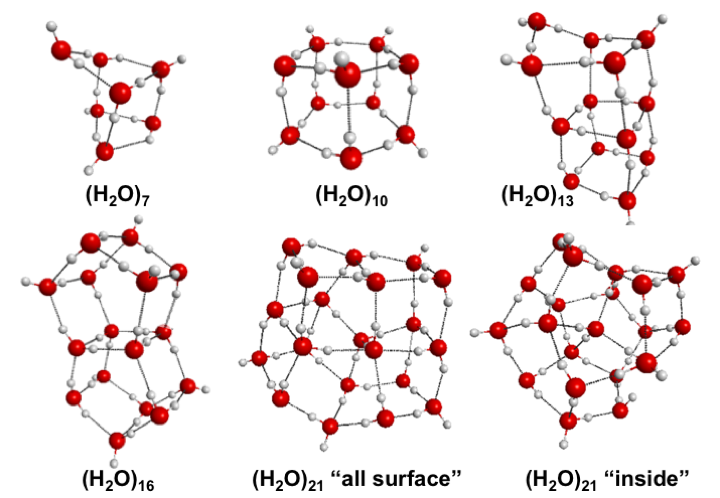
\includegraphics[width=\textwidth]{Figures/Chapter_2/cluster_structures.png}
\caption[Water cluster isomers used in the MBE analysis.]{Water cluster isomers used in the MBE analysis.}
\label{fig:MBE_I_F1}
\end{figure}

\par The calculation of the BSSE correction requires the calculation of the energies of the individual sub-clusters with the basis set functions of all atoms of the cluster, which we refer to as the cluster basis. Using the cluster basis throughout the calculation is the same as performing a counterpoise correction for BSSE involving $N$ bodies.
\par We performed the MBE analysis for selected isomers of the water clusters \ce{(H2O)n}, n = 7, 10, 13, 16, 21.\autocite{lagutschenkov_spectroscopic_2005, yoo_high-level_2010, iwata_cooperative_2013, bulusu_lowest-energy_2006, yoo_structures_2017} We have chosen these clusters because they are of sufficient size that corrections due to BSSE will be significant. Additionally, these clusters are small enough that errors due to numerical imprecisions in the MBE, as pointed out by Herbert \textit{et al.},\autocite{richard_understanding_2014} are negligible at all orders. For n = 21 we considered two geometries, one having all atoms on the surface (“all-surface”) and another in which a single water molecule is fully solvated by its neighbors (“interior”). The geometries of these isomers are shown in Figure \ref{fig:MBE_I_F1}. For \ce{(H2O)7} and \ce{(H2O)_{10}} we performed a full MBE analysis to $n$th order, and this required the evaluation of a total of 127 and 1,023 energies, respectively. For \ce{(H2O)_{13}} the MBE was carried out up to 6-body (4,096 energies). Finally, the MBE was carried out up to 5-body for \ce{(H2O)_{16}} (6,885 energies) and \ce{(H2O)_{21}} (27,896 energies). All calculations were performed at the MP2 level of theory with the family of augmented correlation-consistent basis sets\autocite{dunning_gaussian_1989} aug-cc-pVxZ, x = D, T, Q, 5 (hereafter called AVXZ), as well as with a mixed 5-zeta basis set, which consists of the aug-cc-pV5Z set on the Oxygen and the cc-pV5Z set on the Hydrogen atoms (hereafter referred to as AV5Z/V5Z). In all calculations we ensured there were zero linear dependencies in the basis set so that the complete number of functions were utilized. Each MP2/AVXZ energy calculation was performed at the corresponding MP2/AVXZ geometry except for the calculations with the split AV5Z/V5Z basis set, which were performed at the MP2/AVQZ optimized geometries. The integral thresholds were set at $10^{-15}$ and the HF was converged to at least $10^{-9}$ a.u. All calculations were carried out using the NWChem 6.6 electronic structure software package.\autocite{valiev_nwchem_2010}

\section{Results and Discussion}\label{sec:3_results}
\subsection{Magnitude of many-body terms and their variation with basis set}

\begin{table}[t]
\begin{adjustbox}{width=\columnwidth,center}
\begin{tabular}{@{}ccccccc@{}}
\toprule
 &  \multicolumn{2}{c}{\ce{(H2O)_{20}}}  &  \multicolumn{2}{c}{\ce{(H2O)_{24}}}  &  \multicolumn{2}{c}{\ce{(H2O)_{28}}}\\ \midrule
$k$       & $N_k$        & $n_k $      & $N_k$         & $n_k$          & $N_k$            & $n_k$           \\ \hline
0       & 10,464    & 94       & 65,312     & 2,739       & 429,312       & 17,888       \\
1       & 155,520   & 1,296    & 1,248,912  & 52,038      & 9,619,296     & 400,804      \\
2       & 622,560   & 5,195    & 6,544,680  & 272,777     & 63,529,368    & 2,647,057    \\
3       & 1,086,960 & 9,058    & 15,906,040 & 662,767     & 200,548,656   & 8,356,194    \\
4       & 975,360   & 8,132    & 20,629,752 & 859,716     & 349,190,688   & 14,549,612   \\
5       & 552,096   & 4,604    & 16,889,736 & 703,739     & 388,503,696   & 16,187,654   \\
6       & 184,320   & 1,541    & 8,730,840  & 363,933     & 283,822,656   & 11,825,944   \\
7       & 12,720    & 106      & 2,664,264  & 111,011     & 137,999,376   & 5,749,974    \\
8       & -         & -        & 354,408    & 14,795      & 41,199,552    & 1,716,648    \\
9       & -         & -        & 7,464      & 321         & 6,802,128     & 283,422      \\
10      & -         & -        & -          & -           & 434,376       & 18,099       \\
11      & -         & -        & -          & -           & 1,152         & 48           \\ \hline
Total   & 3,600,000 & 30,026   & 73,041,408 & 3,043,836   & 1,482,080,256 & 61,753,344   \\ \hline
Approx. &           & (30,000) &            & (3,043,392) &               & (61,753,344) \\ \hline
$S_0$      & 0.75482   & -        & 0.75444    & -           & 0.75417       & -            \\ \bottomrule
\end{tabular}
\end{adjustbox}
\begin{spacing}{1.0}
\caption[Number of possible, $N_k$, and non-isomorphic proton configurations, $n_k$, for \ce{(H2O)_{20}}, \ce{(H2O)_{24}} and \ce{(H2O)_{28}} cages. The number of configurations is split into groups depending on the number of (t1d) dimers in the cage, $k$. Notice that $n_k$ is approximately equal to the total number of configurations divided by the order of the symmetry group of the polyhedron, viz. 120, 24 and 24, for the \ce{(H2O)_{20}}, \ce{(H2O)_{24}} and \ce{(H2O)_{28}} cages, respectively.]{Number of possible, $N_k$, and non-isomorphic proton configurations, $n_k$, for \ce{(H2O)_{20}}, \ce{(H2O)_{24}} and \ce{(H2O)_{28}} cages. The number of configurations is split into groups depending on the number of (t1d) dimers in the cage, $k$. Notice that $n_k$ is approximately equal to the total number of configurations divided by the order of the symmetry group of the polyhedron, viz. 120, 24 and 24, for the \ce{(H2O)_{20}}, \ce{(H2O)_{24}} and \ce{(H2O)_{28}} cages, respectively. The residual entropy of each cage is $S_0=k_B\ln(N_k)/N$, where $N$ is the number of molecules in the cage. The Pauling estimate of the residual entropy,  $S_0=0.752\cdot Nk_B$, is slightly smaller than the one derived from explicit enumeration.}\label{tab:MBE_III_T1}
\end{spacing}
\end{table}

\par Table \ref{tab:MBE_I_T1} lists the magnitudes (both uncorrected and BSSE-corrected) of the 1- through n-body terms with the various basis sets for n = 7 and 10. The full MBE up to the 7- and 10-body was carried out for these two clusters respectively, with basis sets from AVDZ to AV5Z/V5Z. For the larger clusters n = 13, 16 and 21 (both “inside” and “all-surface” isomers) the MBE was carried out with just the AVDZ basis set only up to the 6-body for n = 13 and the 5-body for n = 16 and 21, see Table \ref{tab:MBE_I_T2}. For the two isomers of the n = 21 cluster only the uncorrected terms were calculated.

\begin{table}[]
\centering
\begin{tabular}{@{}rrrrrrrrr@{}}
\toprule
     & \multicolumn{4}{c}{Uncorrected}         & \multicolumn{4}{c}{BSSE-corrected}      \\ \midrule
k    & AVDZ    & AVTZ    & AVQZ    & AV5Z/ V5Z & AVDZ    & AVTZ    & AVQZ    & AV5Z/ V5Z \\
\hline
\multicolumn{9}{c}{n = 7}                                                                \\
\hline
1-B  & 2.213   & 2.446   & 2.468   & 2.554     & 2.213   & 2.446   & 2.468   & 2.554     \\
2-B  & -50.578 & -49.459 & -48.626 & -47.160   & -39.894 & -43.958 & -45.712 & -47.165   \\
3-B  & -11.275 & -12.030 & -11.743 & -12.191   & -12.141 & -12.313 & -12.151 & -12.181   \\
4-B  & -1.606  & -1.106  & -0.950  & -0.841    & -0.858  & -0.874  & -0.861  & -0.854    \\
5-B  & 0.493   & 0.194   & 0.043   & 0.013     & 0.021   & 0.021   & 0.020   & 0.023     \\
6-B  & -0.192  & -0.051  & -0.010  & 0.003     & 0.002   & 0.001   & 0.001   & -0.0007   \\
7-B  & 0.037   & 0.008   & 0.002   & -0.0004   & 0.0001  & 0.0001  & 0.0001  & 0.0016    \\
\hline
\multicolumn{9}{c}{n = 10}                                                               \\
\hline
1-B  & 3.952   & 4.509   & 4.449   & 4.595     & 3.952   & 4.509   & 4.449   &           \\
2-B  & -80.165 & -78.707 & -77.249 & -74.796   & -62.762 & -69.504 & -72.387 &           \\
3-B  & -20.475 & -21.285 & -20.790 & -21.625   & -21.691 & -21.989 & -21.582 &           \\
4-B  & -4.742  & -3.028  & -2.202  & -1.878    & -1.968  & -1.978  & -1.923  &           \\
5-B  & 4.698   & 1.200   & 0.219   & -0.038    & 0.012   & 0.015   & 0.014   &           \\
6-B  & -4.081  & -0.964  & -0.179  & 0.071     & 0.040   & 0.041   & 0.039   &           \\
7-B  & 2.175   & 0.708   & 0.1594  & -0.008    & 0.001   & 0.0005  & 0.0005  &           \\
8-B  & -0.707  & -0.324  & -0.0758 & -0.003    & -0.0001 & -0.0001 & -0.0001 &           \\
9-B  & 0.131   & 0.078   & 0.0246  & 0.003     & 0.0000  & 0.0000  & 0.0000  &           \\
10-B & -0.010  & -0.008  & -0.0039 & -0.0006   & 0.0014  & 0.0004  & 0.0000  &           \\ \bottomrule
\end{tabular}
\caption[Magnitudes of the individual terms (kcal/mol) for the clusters \ce{(H2O)n}, n = 7, 10 with the various basis sets. Both the uncorrected and BSSE-corrected values are listed.]{Magnitudes of the individual terms (kcal/mol) for the clusters \ce{(H2O)n}, n = 7, 10 with the various basis sets. Both the uncorrected and BSSE-corrected values are listed.}
\label{tab:MBE_I_T1}
\end{table}

\par We will first discuss the results for the n = 10 cluster as they are representative of the overall pattern observed for all clusters in this study. Figure \ref{fig:MBE_I_F2} compares the magnitudes of the 1- through 10-body terms obtained at the MP2 levels of theory with the various basis sets as well as with the TTM2.1-F interaction potential. The top/bottom panels correspond to the uncorrected/BSSE-corrected terms. The rectangular boxes in the left and middle top/bottom panels indicate the part of each panel that is magnified in the panel immediately on its right side. The uncorrected terms larger than 5-body exhibit an oscillating behavior that is especially magnified for the smaller AVDZ and AVTZ sets, whereas it diminishes for the larger sets. However, this oscillating behavior is not observed for the BSSE-corrected terms (bottom panels in Figure \ref{fig:MBE_I_F2}) as well as the results with the TTM2.1-F interaction potential (not shown here), which seem to track the MP2/AVQZ results quite accurately. These results are better summarized in Figure \ref{fig:MBE_I_F3}, which shows the convergence of the uncorrected (left) and BSSE-corrected (right) 4- through 10-body terms for \ce{(H2O)_{10}} with basis sets. By considering just the uncorrected MP2/AVDZ results (left panel of Figure \ref{fig:MBE_I_F3}), one may arrive at the erroneous conclusion that the MBE expansion is not monotonic, but it oscillates between positive and negative values (which possibly cancel each other), whereas in reality the only surviving terms are the 1- through 4-body ones with the larger terms being practically zero at the CBS limit. The behavior of the many-body terms at the CBS limit is very accurately reproduced even with the smaller AVDZ basis set when the BSSE-correction is applied (right panel of Figure \ref{fig:MBE_I_F3}). Indeed, the 4-body term is essentially constant with all basis sets to ca. –2 kcal/mol (a value close to the uncorrected CBS limit), with all higher terms being practically zero. In this respect, even the MP2/AVDZ BSSE-corrected result accurately reproduces the uncorrected CBS values.

\begin{figure}[t]
\uwsinglespace
\centering
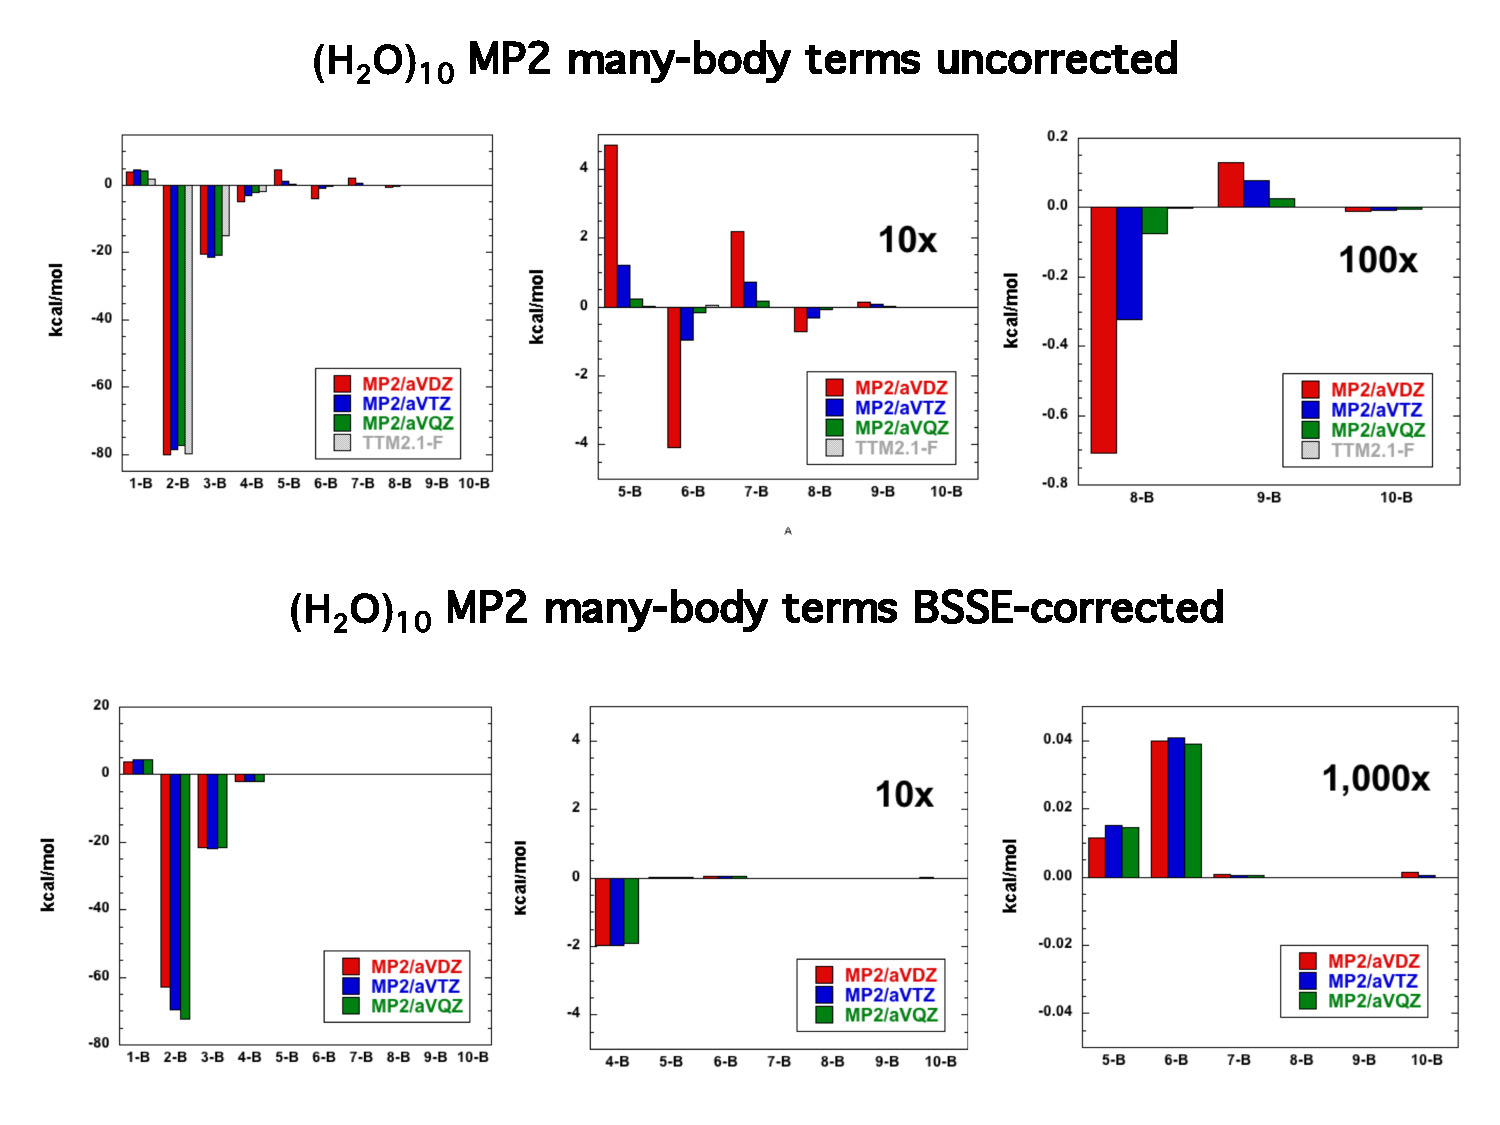
\includegraphics[width=.9\textwidth]{Figures/Chapter_2/W10_MP2_MB.pdf}
\begin{spacing}{1.0}
\caption[Magnitude of the uncorrected (top) and BSSE-corrected (bottom) 1- through 10-body MBE terms for the \ce{(H2O)_{10}} cluster. Note the magnification (10 – 1000X) of the y-axis in the middle and right panels used to indicate the small magnitude of the higher-order relative to the ones for the 2- and 3-body terms.]{Magnitude of the uncorrected (top) and BSSE-corrected (bottom) 1- through 10-body MBE terms for the \ce{(H2O)_{10}} cluster. Note the magnification (10 – 1000X) of the y-axis in the middle and right panels used to indicate the small magnitude of the higher-order relative to the ones for the 2- and 3-body terms.}\label{fig:MBE_I_F2}
\end{spacing}
\end{figure}

\par The same behavior with basis set is found for the uncorrected and BSSE-corrected magnitudes of the many-body terms for \ce{(H2O)7} listed in Table \ref{tab:MBE_I_T1} and shown in Figure \ref{fig:MBE_I_F4}. The convergence patterns are the same as with \ce{(H2O)_{10}} (cf. Figure \ref{fig:MBE_I_F3}), although the magnitudes and corresponding oscillations are smaller than the n = 10 case. This was the reason that we have chosen to discuss the decamer (n = 10) results first as their oscillations around zero are more pronounced than the ones for n = 7. Again, the BSSE-corrected results are quite flat with the size of the basis set to the values that are close to the uncorrected CBS limits, which are also reproduced even with the smaller AVDZ basis set when BSSE-corrections are included. Although we do expect the magnitudes of the many-body terms to scale with cluster size, we do not anticipate their convergence patterns to be different (vide infra).
\begin{figure}[h]
\uwsinglespace
\begin{center}
\begin{minipage}{0.45\textwidth}
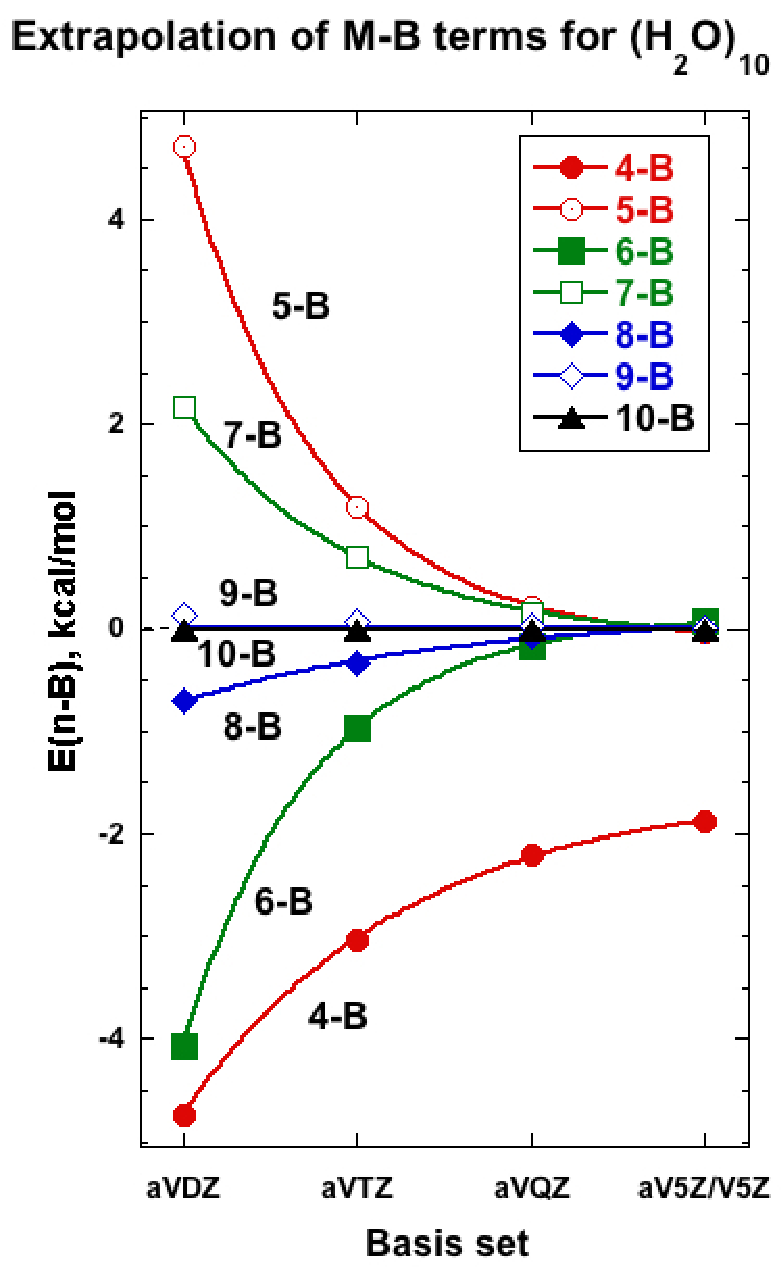
\includegraphics[width=.9\textwidth]{Figures/Chapter_2/MB_extrap_w10_noBSSE.pdf}
\end{minipage}
\begin{minipage}{0.45\textwidth}
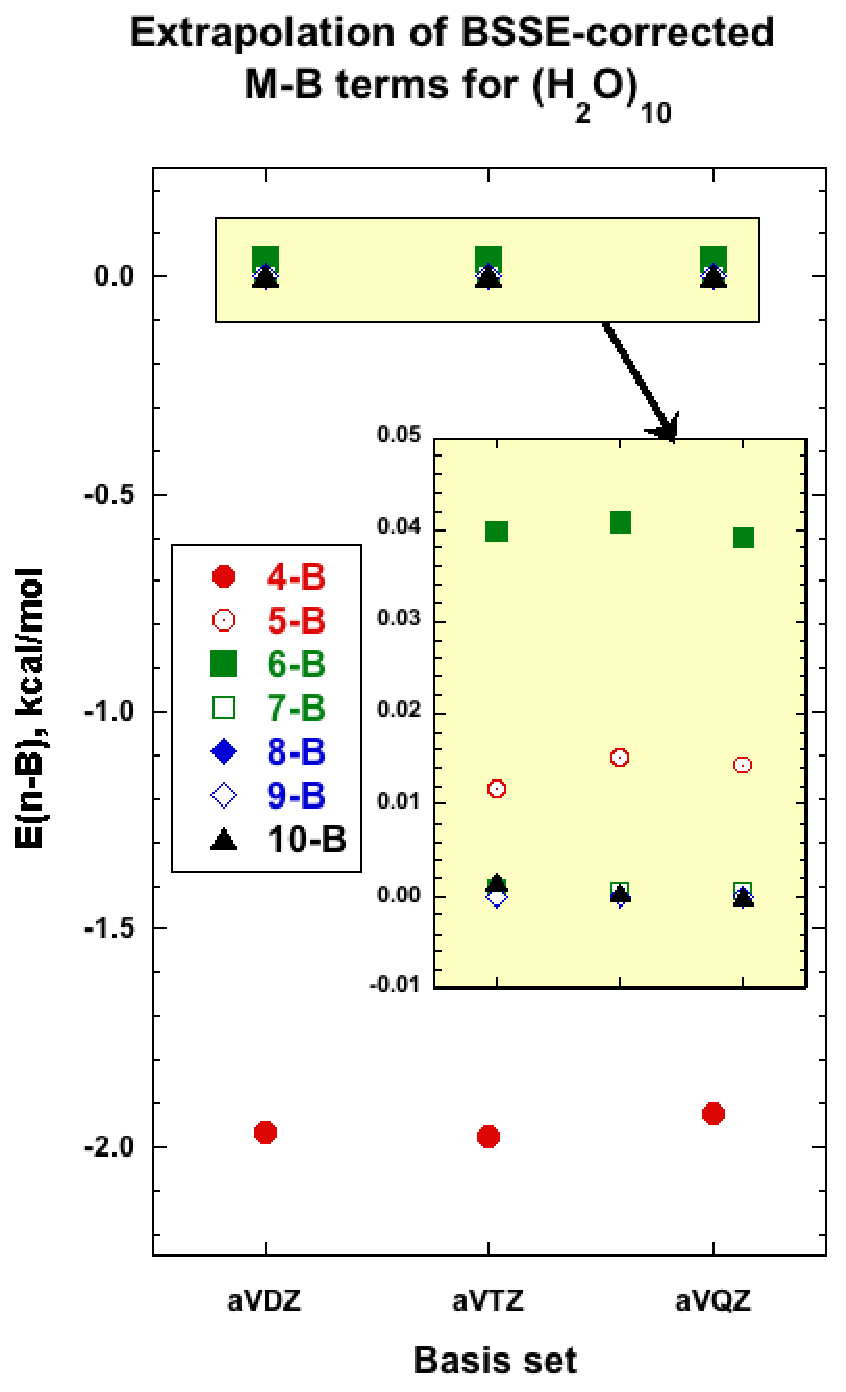
\includegraphics[width=.9\textwidth]{Figures/Chapter_2/MB_extrap_w10_BSSE_all.pdf}
\end{minipage}
\end{center}
\caption[Convergence of the uncorrected (left) and BSSE-corrected (right) 4- through 10-body terms in the many-body expansion for \ce{(H2O)_{10}} for the various basis sets. Notice the different y-axis scales.]{Convergence of the uncorrected (left) and BSSE-corrected (right) 4- through 10-body terms in the many-body expansion for \ce{(H2O)_{10}} for the various basis sets. Notice the different y-axis scales.}
\label{fig:MBE_I_F3}
\end{figure}
\begin{figure}[h]
\uwsinglespace
\begin{center}
\begin{minipage}{0.45\textwidth}
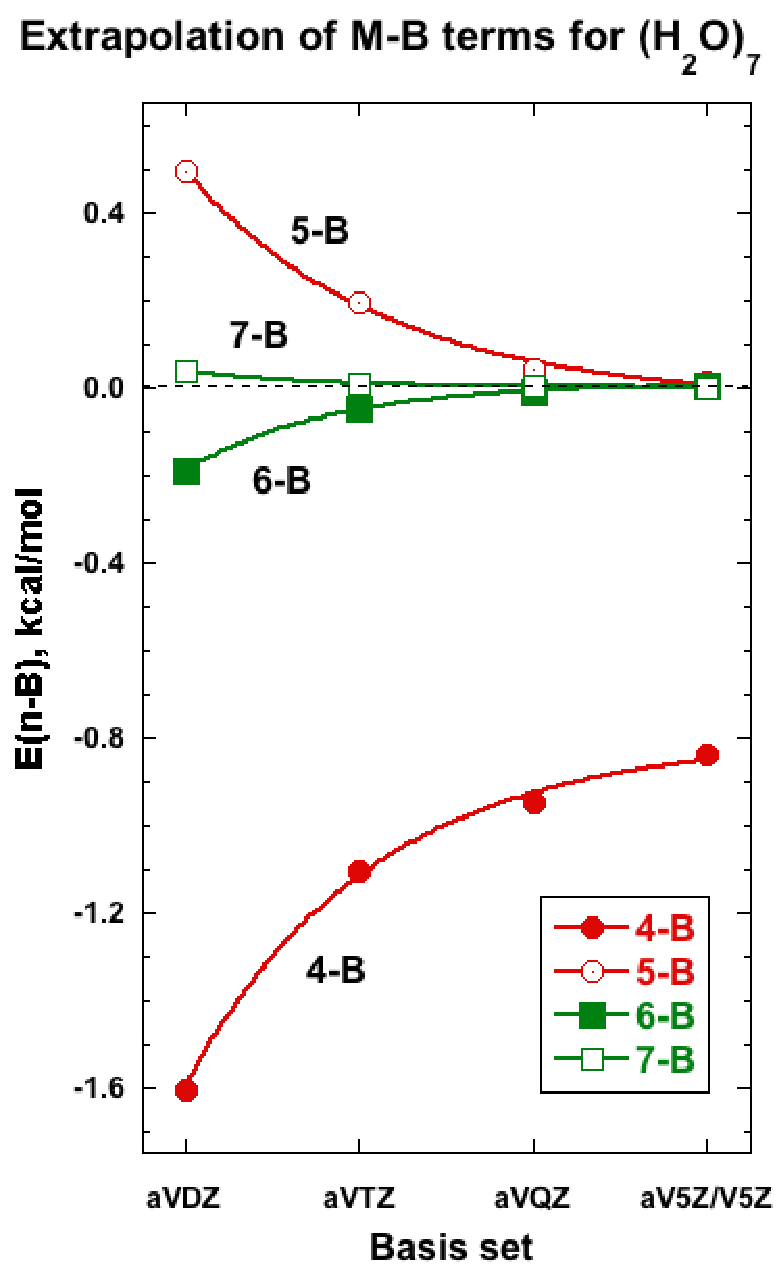
\includegraphics[width=.9\textwidth]{Figures/Chapter_2/MB_extrap_w7_noBSSE.pdf}
\end{minipage}
\begin{minipage}{0.45\textwidth}
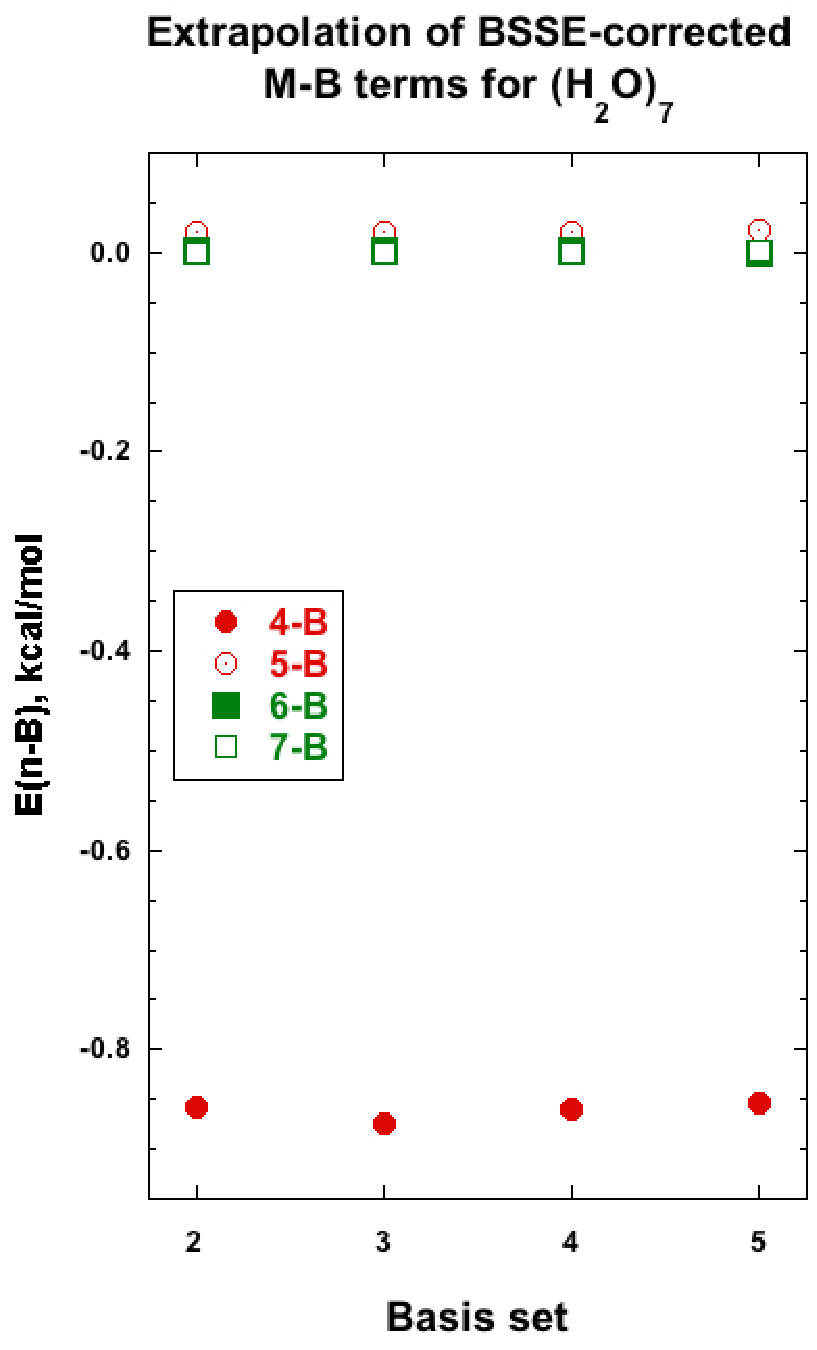
\includegraphics[width=.9\textwidth]{Figures/Chapter_2/MB_extrap_w7_BSSE.pdf}
\end{minipage}
\end{center}
\caption[Convergence of the uncorrected (left) and BSSE-corrected (right) 4- through 7-body terms in the many-body expansion for \ce{(H2O)7} for the various basis sets. Notice the different y-axis scales.]{Convergence of the uncorrected (left) and BSSE-corrected (right) 4- through 7-body terms in the many-body expansion for \ce{(H2O)7} for the various basis sets. Notice the different y-axis scales.}
\label{fig:MBE_I_F4}
\end{figure}
\par The previous results for n = 7 and 10, which suggest that the 5-body and higher terms are truly negligible at the CBS limit, justify the subsequent calculation of the MBE only up to the 6-body term for n = 13 and up to the 5-body term for n = 21. Since it has been previously established that the BSSE-corrected results vary very little with basis set and therefore the MP2/AVDZ numbers are close to both the BSSE-corrected and uncorrected CBS values, we have abstained from carrying out the MBE to full order for n = 13, 16 and 21. Additionally, for the n = 21 isomers we have not estimated the BSSE-corrected terms, since this would require a large number of computations with the full cluster basis set. For example, for n = 21 the 5-body term listed in Table \ref{tab:MBE_I_T2} and shown in Figure \ref{fig:MBE_I_F5} required the computation of 27,896 monomer through pentamer clusters, among them 20,349 pentamer clusters. The BSSE-corrected 5-body term for that cluster would have required the calculation of all these clusters with the full cluster basis set (861 basis functions for the AVDZ basis set). The analysis for the two isomers of n = 21 cluster have been therefore computed in order to confirm the erroneous behavior of the BSSE-uncorrected results for the magnitudes of the many-body terms.
\begin{table}[t]
\begin{adjustbox}{width=\columnwidth,center}
%\centering
\begin{tabular}{@{}ccccc@{}}
\toprule
\multicolumn{5}{c}{$k$-Body Energies of \ce{(H2O)_n} (kcal/mol)} \\ \midrule
$k$ & n=13 & n=16 & n=21 (“all-surface”) & n=21 (“inside”) \\
\hline
1-B & 4.527 (4.527) & 6.456 (6.456) & 7.819 & 9.585 -\\
2-B & -111.096 (-86.692) & -141.072 (-110.162) & -191.747 & -191.447 \\
3-B & -26.264 (-28.335) & -35.514 (-37.944) & -44.152 & -47.359 \\
4-B & -6.352 (-1.499) & -9.463 (-2.179) & -19.892 & -20.976 \\
5-B & 8.243 (0.056) & 14.560 (0.181) & 39.090 & 34.391 \\
6-B & -4.081 (-0.050) & - & - & - \\ \bottomrule
\end{tabular}
\end{adjustbox}
\begin{spacing}{1.0}
\caption[Magnitudes of the individual terms (kcal/mol) for the clusters \ce{(H2O)n}, n = 13, 16, 21 at the MP2/AVDZ level of theory. The BSSE-corrected values are listed in parentheses.]{Magnitudes of the individual terms (kcal/mol) for the clusters \ce{(H2O)n}, n = 13, 16, 21 at the MP2/AVDZ level of theory. The BSSE-corrected values are listed in parentheses.}\label{tab:MBE_I_T2}
\end{spacing}
\end{table}
\par Figure \ref{fig:MBE_I_F5} shows the magnitude (left) and percentage contributions (right) of the 4- to 6-body terms to the MP2/AVDZ binding energies of the clusters n = 7, 10, 13, 16 and 21. The uncorrected (dashed lines) total energies for the 4- through 6-body terms indeed show a large increase with cluster size, while the BSSE-corrected ones (solid lines) yield a small total 4-body term and negligible 5- and 6-body terms. This justifies the assessment that the uncorrected results for the terms larger than 4-body exhibit an erroneous behavior as they increase with cluster size giving unrealistic results for n = 21 and larger clusters. It is interesting to note that the BSSE-corrected 4-body term has an almost constant contribution (\textapprox2\%) to the cluster binding energy up to n = 16 (right panel of Figure \ref{fig:MBE_I_F5}). In this respect, a truncation after the 3-body term will recover \textapprox98\% of the binding energy.
\begin{figure}[h]
\uwsinglespace
\begin{center}
\begin{minipage}{0.45\textwidth}
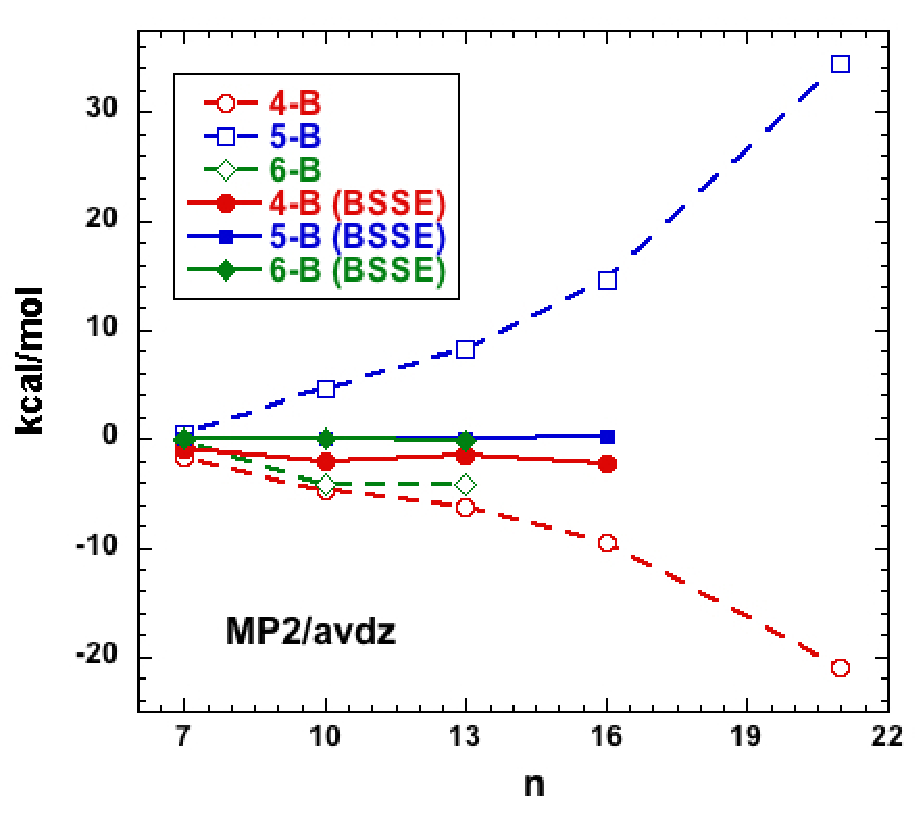
\includegraphics[width=\textwidth]{Figures/Chapter_2/4_B_6_B_vs_n.pdf}
\end{minipage}
\begin{minipage}{0.45\textwidth}
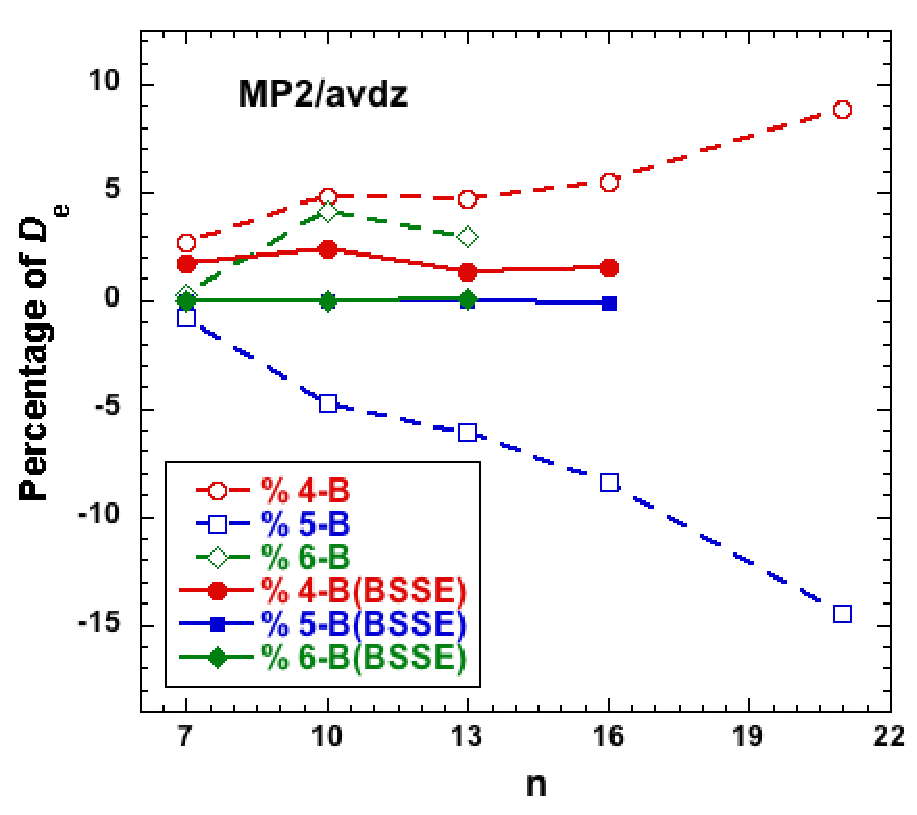
\includegraphics[width=\textwidth]{Figures/Chapter_2/4_B_6_B_perc_vs_n.pdf}
\end{minipage}
\end{center}
\caption[The absolute magnitudes (left) and percentage contributions (right) of the 4- to 6-body terms to the MP2/AVDZ binding energy for (H2O)n, n = 7, 10, 13, 16 and 21. The uncorrected (dashed lines) and BSSE-corrected results (solid lines) are shown.]{The absolute magnitudes (left) and percentage contributions (right) of the 4- to 6-body terms to the MP2/AVDZ binding energy for (H2O)n, n = 7, 10, 13, 16 and 21. The uncorrected (dashed lines) and BSSE-corrected results (solid lines) are shown.}
\label{fig:MBE_I_F5}
\end{figure}
\par Having established that terms beyond the 4-body in the MBE for water clusters are negligible, we now turn our focus to the behavior of the total 2- and 3-body terms. Figure \ref{fig:MBE_I_F6} shows the variation of the uncorrected and BSSE-corrected total 2-body energy for \ce{(H2O)7} and \ce{(H2O)_{10}} with the AVXZ basis sets. The total 2-body term is found to exhibit a similar convergence pattern with basis set size as the one previously reported for individual 2-body terms.\autocite{xantheas_ab_1994,dunning_road_2000,miliordos_n_2015,miliordos_benchmark_2014} As regards the 3-body term, shown in Figure \ref{fig:MBE_I_F7}, its variation and convergence with basis set may not be as systematic as with the 2-body term, however both its total variation and effect of BSSE-corrections are much smaller than the corresponding ones for the 2-body term. In this respect one can consider the 3-body term to be close to convergence and its BSSE-corrected value to be essentially at the CBS limit even with a smaller basis set such as AVDZ.
\begin{figure}[t]
\uwsinglespace
\centering
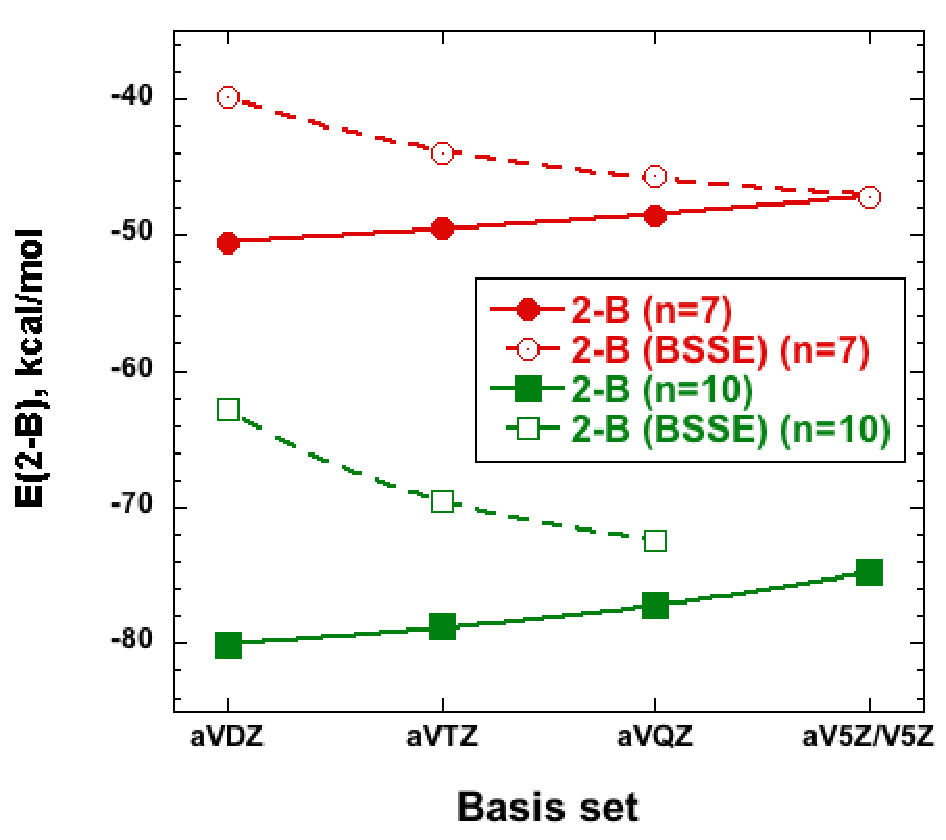
\includegraphics[width=.7\textwidth]{Figures/Chapter_2/E_2B_7_10.pdf}
\begin{spacing}{1.0}
\caption[Convergence of the uncorrected and BSSE-corrected total 2-body energy for \ce{(H2O)7} and \ce{(H2O)_{10}} with the AVXZ basis sets.]{Convergence of the uncorrected and BSSE-corrected total 2-body energy for \ce{(H2O)7} and \ce{(H2O)_{10}} with the AVXZ basis sets.}\label{fig:MBE_I_F6}
\end{spacing}
\end{figure}
\begin{figure}[t]
\uwsinglespace
\centering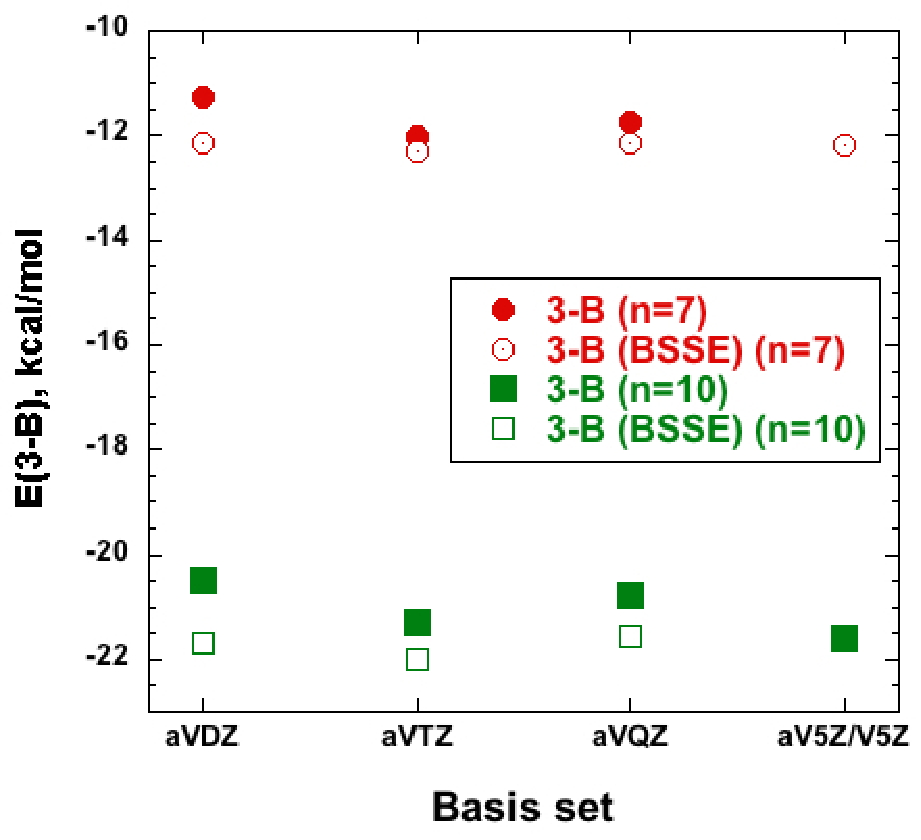
\includegraphics[width=.7\textwidth]{Figures/Chapter_2/E_3B_7_10.pdf}
\begin{spacing}{1.0}
\caption[Convergence of the uncorrected and BSSE-corrected total 3-body energy for \ce{(H2O)7} and \ce{(H2O)_{10}} with the AVXZ basis sets.]{Convergence of the uncorrected and BSSE-corrected total 3-body energy for \ce{(H2O)7} and \ce{(H2O)_{10}} with the AVXZ basis sets.}\label{fig:MBE_I_F7}
\end{spacing}
\end{figure}

\subsection{Origin of the electron correlation component to the cluster binding energy}

\par Let us now turn our attention to the portions of the cluster binding energies which arise due to the HF energy and the electron correlation energy at the MP2 level. These are shown in Figure \ref{fig:MBE_I_F8} for the \ce{(H2O)7} and \ce{(H2O)_{10}} clusters for both the uncorrected and BSSE-corrected cases with the AVXZ basis sets. It is interesting to note that these two clusters have quite similar splits between the HF and the MP2 correlation energy contributions for all basis sets examined in this study. Based on the limited data currently available for these two clusters, we cannot ascertain that this would be a general trend applicable to a wide variety of water cluster sizes having dissimilar hydrogen bonded networks and this will be the subject of a future investigation that will examine whether there are specific types of networks that have large contributions from the HF energy or others which are dominated by the MP2 correlation energy.
\begin{figure}[h]
\uwsinglespace
\centering
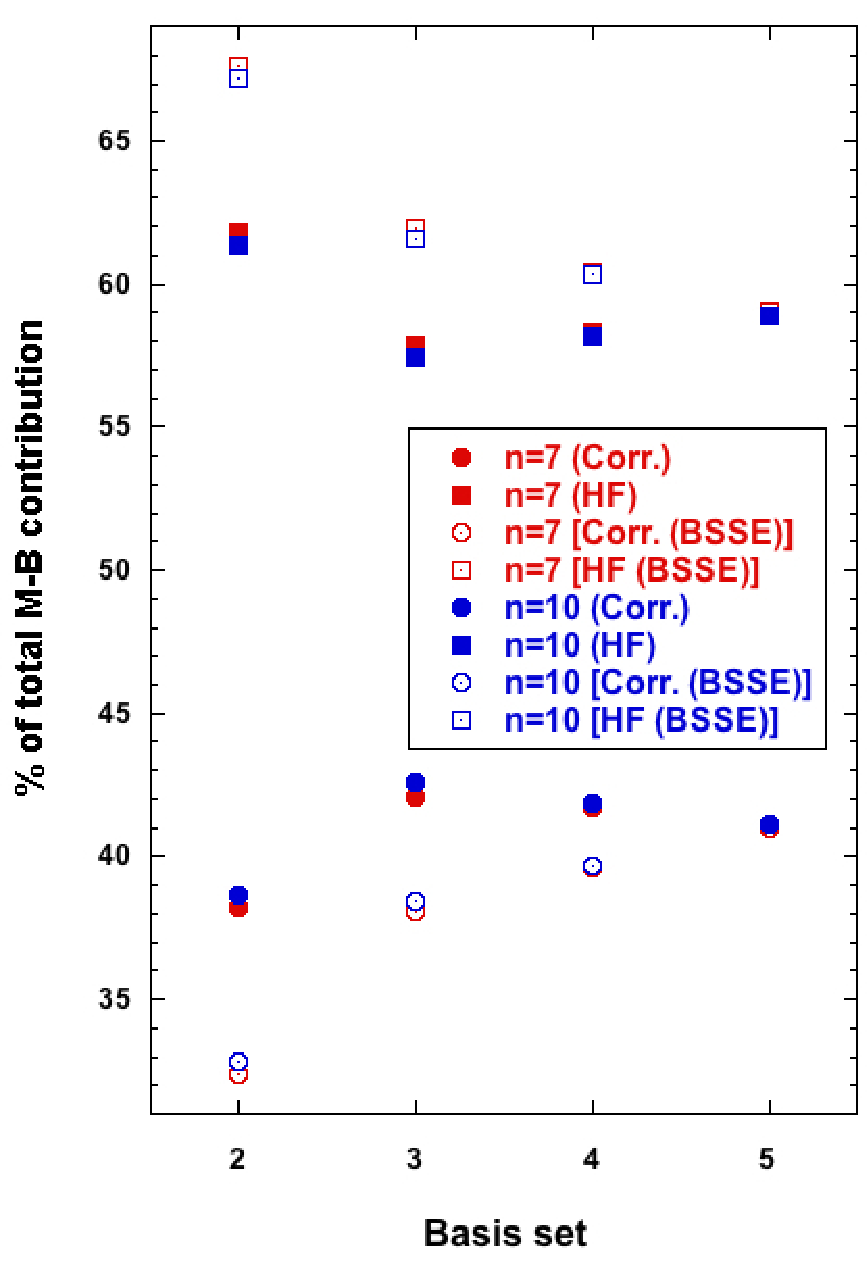
\includegraphics[width=.5\textwidth]{Figures/Chapter_2/percent_corr_HF_7_10.pdf}
\caption[Percentage of the total binding energy from HF and correlation for \ce{(H2O)7} and \ce{(H2O){10}} using the monomer and cluster basis at each of the AVXZ basis sets.]{Percentage of the total binding energy from HF and correlation for \ce{(H2O)7} and \ce{(H2O){10}} using the monomer and cluster basis at each of the AVXZ basis sets.}
\label{fig:MBE_I_F8}
\end{figure}
\par The analysis of our results confirms that the correlation energy component of the cluster binding energy arises primarily from contributions of the 1- and 2-body terms. This can be seen from Table \ref{tab:MBE_I_T3}, which lists the 1-, 2-, and the sum of 3- through 5-body terms for the water clusters containing n = 7, 10, 13 and 16 water monomers which are considered in this study. The entries of Table \ref{tab:MBE_I_T3} represent the results obtained with the largest basis set used for each isomer. These correspond to the AV5Z/V5Z (BSSE corrected) for \ce{(H2O)7}, the AV5Z/V5Z (uncorrected) for \ce{(H2O)_{10}}, and the AVDZ (BSSE corrected) for both the \ce{(H2O)_{13}} and \ce{(H2O)_{16}} clusters. All listed energies are in kcal/mol and the percentage of the total correlation energy at each rank of the MBE is given in parentheses. These results corroborate the proposed scheme by Gora \textit{et al.} known as SAMBA,\autocite{gora_interaction_2011} in which lower levels of theory and basis set can be used at increasing orders of the MBE with only a minimal loss of accuracy.
\begin{table}[]
\centering
\begin{tabular}{@{}ccccc@{}}
\toprule
Cluster & 1-Body          & 2-Body           & Sum of 3- to 5-Body & Total Correlation \\ \midrule
\ce{(H2O)7}  & -3.73 (15.80)   & -19.77 (83.74)   & -0.105 (0.44)       & -23.609           \\
\ce{(H2O)_{10}} & -6.391 (16.59)  & -31.870 (82.75)  & -0.250 (0.65)       & -38.514           \\
\ce{(H2O)_{13}} & -9.135 (23.99)  & -29.0526 (76.31) & 0.135 (-0.35)       & -38.073           \\
\ce{(H2O)_{16}} & -12.051 (24.80) & -36.205 (74.49)  & -0.344 (0.71)       & -48.600           \\ \bottomrule
\end{tabular}
\caption[Contribution of the correlation energy to the various many-body terms for \ce{(H2O)n}, n = 7, 10, 13, 16. The results are obtained with the largest basis set used for each isomer (see text). The percentage of the total correlation energy is given in parentheses. Energies are in kcal/mol, while parentheses indicate the percentage of the total correlation energy.]{Contribution of the correlation energy to the various many-body terms for \ce{(H2O)n}, n = 7, 10, 13, 16. The results are obtained with the largest basis set used for each isomer (see text). The percentage of the total correlation energy is given in parentheses. Energies are in kcal/mol, while parentheses indicate the percentage of the total correlation energy.}
\label{tab:MBE_I_T3}
\end{table}
\par One may also wonder whether the 3-body and higher-order terms actually change significantly in magnitude as higher-order electron correlations are taken into account via e.g. coupled-cluster with single, double, and perturbative triple excitations, CCSD(T). There are two possible changes which should be assessed. The first being the effect of higher-order electron correlations on the minimum energy geometry, and the second being a comparison between the many-body terms calculated at the MP2 and CCSD(T) level for a fixed geometry. In order to assess both of these effects, Table \ref{tab:MBE_I_T4} presents a comparison of the BSSE-corrected and uncorrected 1-, 2-, and 3-body terms for the water trimer, (H2O)3, at the MP2/AVQZ//MP2/AVQZ, CCSD(T)/AVQZ//MP2/AVQZ, and CCSD(T)/AVQZ//CCSD(T)/AVQZ levels of theory. See the caption of Table \ref{tab:MBE_I_T4} for an explanation of this notation.
\begin{table}[t]
\begin{adjustbox}{width=\columnwidth,center}
\begin{tabular}{@{}lccc@{}}
\toprule
(H2O)3       & \multicolumn{1}{p{3cm}}{\centering MP2/AVQZ//\\MP2/AVQZ} & \multicolumn{1}{p{4cm}}{\centering CCSD(T)/AVQZ//\\MP2/AVQZ} & \multicolumn{1}{p{4cm}}{\centering CCSD(T)/AVQZ//\\CCSD(T)/AVQZ}\\
\hline
\textbf{Total Energy} & \textbf{-15.440}   & \textbf{-15.478}       & \textbf{-15.493}           \\
\hline
1-B          & 0.429              & 0.410                  & 0.346                      \\
2-B          & -13.359            & -13.428                & -13.479                    \\
3-B          & -2.510             & -2.460                 & -2.360           \\ \bottomrule         
\end{tabular}
\end{adjustbox}
\begin{spacing}{1.0}
\caption[The MP2/AVQZ and CCSD(T)/AVQZ 1-, 2-, and 3-body terms for \ce{(H2O)3} at the MP2/AVQZ and CCSD(T)/AVQZ geometries. The notation CCSD(T) /AVQZ//MP2/AVQZ means CCSD(T)/AVQZ energies are calculated the MP2 /AVQZ optimized geometry. The relevant monomer reference energies (from left to right), in a.u., are -76.35191864, -76.36358738, and -76.3635876.]{The MP2/AVQZ and CCSD(T)/AVQZ 1-, 2-, and 3-body terms for \ce{(H2O)3} at the MP2/AVQZ and CCSD(T)/AVQZ geometries. The notation CCSD(T)/AVQZ//MP2/AVQZ means CCSD(T)/AVQZ energies are calculated the MP2/AVQZ optimized geometry. The relevant monomer reference energies (from left to right), in a.u., are -76.35191864, -76.36358738, and -76.3635876.}\label{tab:MBE_I_T4}
\end{spacing}
\end{table}
\par In the case of the trimer, using CCSD(T)/AVQZ at the MP2/AVQZ geometry decreases the 3-body term from -2.510 kcal/mol to -2.460 kcal/mol. This number decreases by an additional 0.1 kcal/mol to -2.360 kcal/mol when the same calculations are carried out at the CCSD(T)/AVQZ optimized geometry. From this, we can conclude that the effects of using a CCSD(T) geometry are larger than that of using CCSD(T) energies at an MP2 geometry. Additionally, these calculations demonstrate that CCSD(T), both in terms of geometry and energy, tend to decrease the magnitude and percentage of the 3-body term. Although it is not clear that these observations have been stated explicitly in the past, they can be inferred from the fact that the O-O distances in MP2 geometries tend to be smaller than those of the corresponding CCSD(T) geometry\autocite{miliordos_optimal_2013}.
\begin{table}[t]
\begin{adjustbox}{width=\columnwidth,center}
\begin{tabular}{@{}ccccc@{}}
\toprule
             & MP2/AVDZ          & CCSD(T)/AVDZ               & MP2/AVTZ          & CCSD(T)/AVTZ \\
             \hline
Total Energy & \textbf{-60.908 / -50.658} & \textbf{-60.841 / -49.900} & \textbf{-59.998 / -54.676} &              \\
\hline
1-B          & 2.213 / 2.213     & 2.075 / 2.075              & 2.446 / 2.446     & 2.372        \\
2-B          & -50.578 / -39.894 & -50.727 / -39.359          & -49.459 / -43.958 & -49.738      \\
3-B          & -11.275 / -12.141 & -10.811 / -11.710          & -12.030 / -12.313 & -11.636      \\
4-B          & -1.606 / -0.858   & -1.758 / -0.937            & -1.106 / -0.874   &              \\
5-B          & 0.493 / 0.021     & 0.553 / 0.027              & 0.194 / 0.021     &              \\
6-B          & -0.192 / 0.002    & -0.212 / 0.002             & -0.51 / 0.001     &              \\
7-B          & 0.037 / 0.000     & 0.040 / 0.000              & 0.008 / 0.000     &             \\ \bottomrule
\end{tabular}
\end{adjustbox}
\begin{spacing}{1.0}
\caption[The MP2/AVXZ and CCSD(T)/AVXZ BSSE-uncorrected and BSSE-corrected interaction energies for \ce{(H2O)7} in the format $E_{uncorr}$ / $E_{corr}$ all carried out at the MP2/AVXZ geometry for X=D, T. The relevant water monomer reference energies (from left to right), in a.u., are -76.26090977, -76.27390289, -76.3289924, and -76.34232562. We do not report the BSSE-corrected numbers for CCSD(T)/AVTZ due to the computational expense.]{The MP2/AVXZ and CCSD(T)/AVXZ BSSE-uncorrected and BSSE-corrected interaction energies for \ce{(H2O)7} in the format $E_{uncorr}$ / $E_{corr}$ all carried out at the MP2/AVXZ geometry for X=D, T. The relevant water monomer reference energies (from left to right), in a.u., are -76.26090977, -76.27390289, -76.3289924, and -76.34232562. We do not report the BSSE-corrected numbers for CCSD(T)/AVTZ due to the computational expense.}\label{tab:MBE_I_T5}
\end{spacing}
\end{table}
\par We also report the CCSD(T)/AVDZ and CCSD(T)/AVTZ energies at the corresponding MP2 geometries in Table \ref{tab:MBE_I_T5}. We find the same trend in this case as with the trimer. In this case, however, we can look at all of the 3- to 7-body terms to assess if any of these terms increase as higher-order electron correlations are included. We find, however, that the sum of these many-body terms decreases relative to the MP2 calculations, and that the 3-body decreases in magnitude and percentage, as in the case of \ce{(H2O)3}.

\begin{figure}[t]
%\uwsinglespace
\begin{center}
\includegraphics[width=.5\textwidth]{Figures/Chapter_2/2body_bsse_decay_with_basis.tif}
\end{center}
\begin{spacing}{1.0}
\caption[Variation of the BSSE correction for the 2-body terms with the O-O distance between fragments with the different basis sets used in this study. Solid lines represent least mean squares fits of the data to the function $a(1+erf(-bR_{OO}))$ for each basis set.]{Variation of the BSSE correction for the 2-body terms with the O-O distance between fragments with the different basis sets used in this study. Solid lines represent least mean squares fits of the data to the function $a(1+erf(-bR_{OO}))$ for each basis set.}\label{fig:MBE_I_F9}
\end{spacing}
\end{figure}
\begin{figure}[t]
%\uwsinglespace
\begin{center}
\includegraphics[width=.5\textwidth]{Figures/Chapter_2/2body_bsse_correlation.tif}
\end{center}
\begin{spacing}{1.0}
\caption[Predicted versus calculated BSSE correction for the individual 2-body terms of the clusters with the different basis sets used in this study.]{Predicted versus calculated BSSE correction for the individual 2-body terms of the clusters with the different basis sets used in this study.}\label{fig:MBE_I_F10}
\end{spacing}
\end{figure}

\par It is worth noting the small magnitude and associated percentage contribution of the 3-body and higher-order terms to the total correlation energy component of the binding energy. Notice that for the \ce{(H2O)_{13}} and \ce{(H2O)_{16}} clusters, for which calculations have not been performed with basis sets large enough to arrive at the CBS limit, this percentage is larger because the 2-body term overshoots the CBS limit when computed with the full cluster basis. This finding can have significant ramifications in terms of the utility of the 3-body and higher-order terms for applications in very large systems. Earlier, we determined that the use of BSSE-corrected 3-body and higher order terms with even the AVDZ basis set is justified. Our analysis further suggests that even using only the HF contribution for the 3-body and higher order terms does not result in a significant error. Recall that the percentages listed in parentheses in Table \ref{tab:MBE_I_T3} are those of the overall contribution of correlation to the cluster binding energy, and Figure \ref{fig:MBE_I_F5} shows that this is only \textapprox40\% of the total binding energy. Thus, for these neutral water systems, neglecting the correlation contribution in all terms above the 3-body results in an error of $O$(0.1\%). In future studies we intend to apply this analysis to ionic aqueous clusters, for which one might expect that the correlation contribution will be even smaller since the 2-body term should become larger.

\subsection{Analytic expressions for the 2-body BSSE correction}

\par The BSSE correction between two bodies (fragments), estimated via the Boys-Bernardi function CounterPoise (fCP) method,\autocite{boys_calculation_1970} is based on the premise that basis functions on one fragment help lower the energy of the other fragment and vice versa. Equivalently, because the basis set on one fragment is far from being complete, it needs to “borrow” functions from neighbors for a better description of its Hilbert space. Naturally, this need to “borrow functions from the neighbor” diminishes as the basis set becomes larger and it is formally zero at the (unattainable) basis set limit (i.e. when complete sets of basis functions describe the Hilbert space on each fragment). Additionally, since these basis functions are centered on the individual atoms, it becomes reasonable to assume that an obvious descriptor of the ease to lower the energy of neighbors by lending basis functions is a distance criterion. The fact that the basis sets employed in this study have diffuse functions with long tails adds to the concept of the overlap of the charge distributions between neighboring fragments.

\par For a pair of Gaussian functions, whose centers are separated by $R$, it can be shown (see Appendix) that their overlap area is proportional to $a(1+erf(-bR))$, eq. \eqref{eq:MBE_I_2} in the Appendix. Figure \ref{fig:MBE_I_F9} shows the variation of the BSSE correction for all 219 2-body energies of the various clusters with R(O-O) for the various basis sets considered in this study (symbols) and their fit to eq. \eqref{eq:MBE_I_2} (lines). The 3 groupings of the points with R in Figure \ref{fig:MBE_I_F9} represent the first, second and third nearest neighbor pairs, respectively. The values of the constants $a$, $b$, determined by a least-squares fit of the data to eq. \eqref{eq:MBE_I_2}, as well as the quality of the fit for the various basis sets are listed in Table $\ref{tab:MBE_I_T4}$. The value of $a$ shows a systematic reduction with increasing basis set by \textapprox65\% (AVDZ to AVTZ) and \textapprox58\% (AVTZ to AVQZ), while the value of $b$ remains at about 0.5 along this series [note the factor of $1/2\sqrt{2}$ in eq. \eqref{eq:MBE_I_1}]. In contrast, the values of $a$, $b$ for the AV5Z/V5Z basis are well outside this trend, a fact that may suggest that the heuristic model used to estimate the BSSE correction probably breaks down for this large basis set.

\par Nevertheless, the fits to eq. \eqref{eq:MBE_I_2} suggest that the BSSE correction can be accurately estimated without the actual calculation being performed. Figure \ref{fig:MBE_I_F10} shows the estimated, via eq. \eqref{eq:MBE_I_2}, versus the calculated BSSE correction for all 219 2-body terms for all clusters obtained with the basis sets used in this study. The agreement is satisfactory to indeed support the thesis of obtaining an accurate 2-body term from the uncorrected value by adding the BSSE correction via eq. \eqref{eq:MBE_I_2}.

\section{Conclusions}\label{sec:3_conclusions}

\par Typical MP2 calculations with the AVDZ basis set of the many-body, non-additive terms for medium size clusters (n\textless 10) yield a large oscillating behavior of their magnitudes that may have cast doubt on the convergence of the MBE for water. Our analysis of the n = 7, 10, 13, 16 and 21 clusters, extending the basis set to the CBS limit, suggests that the increasing magnitude of the 5-body and larger terms with cluster size is an artifact of the basis set size since their magnitude decreases with increasing basis set converging to practically zero at the CBS limit. Therefore, the fact that the size of a particular term with a small basis set is large does not necessarily mean that it will remain important upon performing a more accurate calculation with a larger basis set. The need to use a very large basis set in order to accurately capture the many-body terms in water presents a serious problem in their accurate calculation for large systems, since very large basis sets need to be employed. However, the problem is successfully addressed upon the inclusion of BSSE corrections. The BSSE-corrected magnitudes of the many-body terms are almost constant with basis set size and furthermore the BSSE-corrected magnitudes of these terms, even with the smaller AVDZ basis set, are quite close to the CBS limit. 
\par Our results suggest that the 3-body term is essentially converged to the CBS limit when an AVDZ basis is used and the BSSE correction is taken into account. The BSSE-corrected 4-body term is almost constant (\textapprox2\%) for the cluster sizes considered in this study (n = 7, 10, 13, 16). Therefore, the MBE truncated at the 3-body term can yield cluster binding energies with \textapprox98\% accuracy. Furthermore, we have shown that over 99\% of the contribution from the correlation energy is captured by 1-body and 2-body terms alone.
\par Our results lay the groundwork for accurate and reliable, on-the-fly, \textit{ab initio}, many-body molecular dynamics of complex systems. One can envision using the highest-level method affordable for the 1- and 2-body terms in conjunction with just the HF contribution to the 3- and even to the 4-body terms. This scheme is expected to produce high-level ab initio energies that are close to the quality of the highest-level method used for the 1- and 2-body terms. Additional studies of the distance-dependence of BSSE corrections are required so that a prescription for estimating BSSE-corrections in systems relevant to molecular dynamics can be made confidently. That is, while strides have been made toward removing BSSE without the cost of using the cluster basis,\autocite{richard_understanding_2018,ouyang_many-body_2015,mayer_many-body_2017} it is not clear that methods like these are practical for the case of a periodic simulation of water. Clearly, in such a large system, the full basis of the unit cell cannot be used, nor can one expect to be able to perform the many, very-small calculations required by the methods of BSSE-correction proposed in Refs. \cite{richard_understanding_2018,ouyang_many-body_2015,mayer_many-body_2017}. It is our belief that further work on many-body BSSE corrections should bear in mind the difficulties associated with correcting for BSSE in extremely large systems. We anticipate something akin to the geometrical counter-poise method\autocite{kruse_geometrical_2012} is practical for use in a condense-phase simulation, and we will explore improvements on this type of method in the future.

\section{Appendix}

Consider two Gaussian distribution functions 
$$f(x;\mu, \sigma^2)=\frac{1}{\sigma\sqrt{2\pi}}e^{\frac{-(x-\mu)^2}{2\sigma^2}},$$
where $\mu$ is the center and $\sigma^2$ the variance, centered at $\mu_1=0$ and $\mu_2=R$ with $\sigma^2=1$, viz.
$$
f(x;0, 1)=\frac{1}{\sqrt{2\pi}}e^{\frac{-x^2}{2}}
$$

and

$$
f(x;R, 1)=\frac{1}{\sqrt{2\pi}}e^{\frac{-(x-R)^2}{2}}.
$$

Their intersection point $x_C(0<x_C<R)$, determined by the condition $f_1(x_C)=f_2(x_C)$, is $x_C=R/2$. The area under a Gaussian function is $1/2erf((x-\mu)/\sqrt{2})$, therefore the common (overlapping) shaded area  between the two Gaussians is
$$
A=1-\frac{1}{2}erf\left(\frac{x_C}{\sqrt{2}}\right)+\frac{1}{2}erf\left(\frac{x_C-R}{\sqrt{2}}\right)
$$

or by substituting $x_C=R/2$,
\begin{equation}\label{eq:MBE_I_1}
    A=1+erf\left(\frac{-R}{2\sqrt{2}}\right).
\end{equation}

The BSSE correction for the individual 2-body terms is fit to the function
\begin{equation}\label{eq:MBE_I_2}
    \mathrm{BSSE}=a(1+erf(-bR))
\end{equation}
where $a$ and $b$ are constants.


\chapter{The many-body expansion for aqueous systems: II. Alkali metal and halide ion-water interactions}
\label{ch:MBE_II}

\section{Introduction}
\par The Many-Body Expansion (MBE) underpins a number of recent many-body, non-additive classical potential energy surfaces, especially those involving water\autocite{burnham_development_2002,fanourgakis_flexible_2006,fanourgakis_development_2008,heindel_benchmark_2018,wang_flexible_2011,babin_development_2013,das_development_2019,gora_predictions_2014} that are fitted to ab-initio data for clusters. While the concept of the MBE has resulted in some of the most accurate classical interaction potentials created to date, these potentials only exist for a relatively narrow range of systems for which they were parametrized. Most notably, there is an ever-present interest in understanding the details of molecular interactions between water and various solutes, such as ions. There is also interest in elucidating the effects of these ions, especially in higher concentrations, in modifying the interactions among neighboring water molecules and how this alters the resulting dynamics of these systems. Additionally, the interactions between water and ions are paramount in understanding the physical mechanisms behind many chemical and biological processes such as aqueous solvation\autocite{makarov_solvation_2002,collins_ions_2004}, ion channels\autocite{pinto_influenza_1992,shearman_modulation_1989} and electrochemistry.\autocite{zhang_effects_2011,liu_doping_2006,tang_dynamic_2011}

\par Ions have been known to alter the local hydrogen bonding network in water by inducing local disruptions depending on their charge state.\autocite{marcus_ions_2015,chang_recent_2006,hribar_how_2002} Positively charged ions attract neighboring water molecules as acceptors (A) via their oxygen atoms, whereas negatively charged ones as donors (D) via their hydrogens. The distinct local arrangement of the nearest-to-ion-neighbor water molecules (i.e., the first solvation shell) induces a local structure in subsequent solvation shells away from the ion. For example, in the case of positively charged ions the first solvation shell water molecules participate in hydrogen bonds with molecules in the second solvation shell exclusively as (D), whereas for negatively charged ions as both (D) and (A). Nevertheless, the effect of the ions in altering the interaction between neighboring water molecules in clusters has been quantified by both experimental infrared and computational ab-initio studies. The former record the changes of the red shifts in the OH stretching vibrational bands that occur due to the strengthening/weakening of the hydrogen bonds,\autocite{horvath_anharmonicities_2010,bush_infrared_2008,duncan_spectroscopy_1997,ayotte_spectroscopic_1999,dorsett_probing_1999} while the latter provide quantitative information about the change in the two-body water-water interaction due to the presence of a nearby ion.\autocite{xantheas_theoretical_1995,xantheas_quantitative_1996}

\par Ions are also known to affect the structure and overall stability of solutes in aqueous environments. For example, the extent to which an ion affects processes involving a protein, which was first realized in 1888,\autocite{hofmeister_zur_1888} is described by the Hofmeister series. In other cases, the ion identity greatly affects the rates and even outcomes of certain biological processes,\autocite{zhang_interactions_2006} with the molecular level mechanism responsible for these changes still not fully understood. The view that the ions affect processes in aqueous environments by disrupting the hydrogen-bonding network of water\autocite{marcus_effect_2009} has resulted into their categorization to “structure-makers” or “structure-breakers”.\autocite{collins_hofmeister_1985} The notion that ions can have long-range effects on the hydrogen-bonding network of liquid water is supported by previous spectroscopic\autocite{omta_influence_2003,omta_negligible_2003,kropman_vibrational_2003,kropman_effect_2004} and thermodynamic\autocite{batchelor_impact_2004} studies with some recent studies even suggesting that a single ion has an influence on millions of surrounding water molecules.\autocite{chen_electrolytes_2016} Spectroscopic 2-D infrared measurements in the region of the OD stretch in HDO molecules in the presence of various ions aim at measuring the orientational correlation time of water outside the first solvation shell of the ions. More recent 2-D Raman-THz measurements, which directly probe the intermolecular hydrogen-bond stretching region, provide support for the structure-making and structure-breaking scenarios by correlating the relaxation time of the stretch to the B-coefficient of the cation in solution.\autocite{shalit_terahertz_2017} The authors conclude that this correlation “confirms the empirically used concept of structure makers or structure breakers on a molecular level.”\autocite{shalit_terahertz_2017} However, some disagreement over whether or not, and to what extent, various ions affect the long range hydrogen-bonding network of bulk aqueous ionic solutions still remains. Attempting to perform and interpret experiments in regions far away from the ion, especially in concentrated ionic solutions remains a fundamental challenge.

\par Experimental relaxation times from 2-D Raman-THz measurements suggested a rather strong correlation to the properties of the cation while being insensitive to the anion; for instance, \ce{SrCl2} vs. \ce{SrBr2} has no measurable effect on the relaxation time.\autocite{shalit_terahertz_2017} This is in direct contrast to the conventional wisdom that the anion produces the larger Hofmeister effect due to the dominating role of ionic dispersion at larger ionic concentrations and near interfaces.\autocite{bostrom_why_2004,jungwirth_molecular_2001,jungwirth_ions_2002,dang_molecular_2002,garrett_ions_2004} Therefore, it has been rationalized that anions should be the more important species due to their greater polarizabilities relative to the cations.\autocite{yang_hofmeister_2009} On the other hand, one might expect a cation to have a much greater effect on the surrounding hydrogen-bonding network of water due to the fact that cations must be stabilized via the oxygen atom, rather than donation of electron density via the hydrogen atom as in normal hydrogen bonds.\autocite{kwan_effect_2019} We will discuss ramifications of this effect in more detail later, when we present an anomaly arising in the presence of a cation but not an anion.

\par The previous discussion suggests that ion specificity plays a crucial role in determining the properties of aqueous ionic systems. To this end, the accurate description of the underlying interactions plays a crucial role in rendering a molecular level picture of the origin of these effects. The field of developing classical potentials for ion-water interactions has been active for the last 30 years\autocite{probst_molecular_1985,limtrakul_solvent_1985,probst_study_1987,amira_molecular_2004,wick_computational_2009,wick_molecular_2008} with efforts continuing up to this day.\autocite{arismendi-arrieta_i-ttm_2015,bajaj_toward_2016,riera_i-ttm_2016} Advances in computer hardware and software have also allowed for electronic structure driven molecular dynamics\autocite{car_unified_1985,kuhne_second_2014} simulations of aqueous ionic solutions,\autocite{todorova_carparrinello_2008,bako_carparrinello_2002,bankura_hydration_2013,baer_local_2016,duignan_quantifying_2020} so that a separate parameterization is not required for each ion but rather depends upon the level of electronic structure theory used. Nevertheless, the ensuing dynamics need to be propagated via the many-body terms in order to reduce the computational cost associated with these simulations while still allowing the use of a high level of theory.\autocite{liu_hydrogen-bond_2018,liu_variational_2019} 

\par In a previous paper\autocite{heindel_many-body_2020} (hereafter referred to as paper MBE-I) we have investigated the convergence of the many-body terms for water clusters with the level of electron correlation and basis set. We found that 5-body and higher terms converge monotonically to zero upon increasing the basis set towards the Complete Basis Set (CBS) limit and this behavior is accurately reproduced even with the smaller (aug-cc-pVDZ) set when the Basis Set Superposition Error (BSSE) is taken into account. In addition, it was found that neglecting the correlation contribution in all terms above the 3-body resulted in an error of the order of 0.1\%. Most importantly, the BSSE correction for the largest 2-body term in the MBE followed very closely the relation $a(1+erf(-bR))$, where $R$ is the distance between the two (either nearest or distant) oxygen atoms of the corresponding dimer. In the present paper we build upon these previous findings by extending the study of the MBE terms for ion-water clusters. We present detailed calculations focusing on the many-body terms of ionic clusters incorporating either a positive or negative ion on both the inside and outside of the cluster with a specific emphasis of how the guest ion changes the water-water interaction in the host’s hydrogen bonding network. The paper is organized as follows. In Section \ref{sec:MBE_2_sec_2} we describe our approach and outline the computational details used in this study. In Section \ref{sec:MBE_2_sec_3} we present the variation of the many-body terms with basis set as well as the BSSE corrections and their fitting to a universal function. Final conclusions are drawn in Section \ref{sec:MBE_2_sec_4}.

\section{Approach and Computational Details} \label{sec:MBE_2_sec_2}
\par We have extensively described the methods by which we perform the MBE in the preceding publication of this series\autocite{heindel_many-body_2020} as well as in earlier publications,\autocite{xantheas_ab_1994,xantheas_cooperativity_2000} so we will only briefly review the pertinent details here. The MBE is a means of decomposing some molecular property into contributions from various fragments of the total system. In the case of the total interaction energy, $D_e$, which is our focus in this work, the MBE can be cast as,\autocite{xantheas_ab_1994,xantheas_cooperativity_2000,hankins_water_1970}
$$
D_e=\sum_{i=1}^nE_{iB}=E(1,2,...,n)-\sum_{i=1}^nE_{ref,i}
$$
where $E_{ref,i}$ is the reference energy of the isolated fragment $i$. Furthermore, each of the $i$-body terms, $E_{iB}$, can be written as,
$$
E_{1B}=\sum_{i=1}^n[E(i)-E_{ref,i}]
$$
$$
E_{2B}=\sum_{i<j}[E(i,j)-E(i)-E(j)]
$$
$$
E_{3B}=\sum_{i<j<k}[E(i,j,k)-E(i,j)-E(i,k)-E(j,k)+E(i)+E(j)+E(k)]
$$

and so on for the $4$- through $n$-body terms. In the above notation, the term $E(i,j,k)$ corresponds to the energy of a trimer containing fragments $i$, $j$, and $k$.

\par The various energy terms are computed at some level of electronic structure theory with an atom-centered basis set, which is usually far from being complete. This introduces the additional complication of the Basis Set Superposition Error (BSSE), i.e. the compensation of each fragment’s basis set incompleteness by using functions from the basis set of its neighbors. The error due to this effect is estimated by computing all energies in the presence of the basis functions of the full system.\autocite{richard_understanding_2018,boys_calculation_1970,xantheas_importance_1996}

\par In this work we compute the MBE terms for aqueous clusters of alkali metal \ce{M} = \ce{Li^+}, \ce{K^+}, \ce{Cs+} and halide \ce{X} = \ce{Cl^-}, \ce{Br^-}, and \ce{I^-} clusters. We chose the cluster size of 10 fragments, \ce{Z^{+/-}(H2O)9}, in order to directly compare the results with the ones previously reported for a water cluster of the same number of “bodies”, \ce{(H2O)_{10}}. Our previous study (paper MBE-I) indicated that this cluster is large enough that certain artifacts attributed to BSSE are more evident and in addition we can meaningfully distinguish between the “ion-inside” and “ion-outside” isomers of the cluster. The two topologically different isomers correspond to the two cases when the ion resides on the surface or the inside of the water cluster. These geometries were selected by running NVT molecular dynamics trajectories with the Dang-Chang potential\autocite{dang_molecular_1997} and choosing frames in which the ion was clearly on the inside or outside of the structure and then optimizing these structures at the MP2/aug-cc-pVXZ level of theory (X = D, T, Q, 5). We will hereafter refer to Dunning’s augmented correlation consistent basis sets\autocite{dunning_gaussian_1989,wilson_gaussian_1999,woon_gaussian_1993} as aVXZ (X = D, T, Q, 5). In the case of \ce{Cl^-(H2O)9}, \ce{Br^-(H2O)9}, and \ce{I^-(H2O)9} we did not find any frames in which the ion clearly resided on the inside of the cluster. Therefore, we constructed a constrained structure in which the halide ion is tetrahedrally coordinated by four water molecules, and the remaining five water molecules are attached to this first solvation shell. All degrees of freedom were then allowed to relax during the optimization subject to the condition that the chloride remains tetrahedrally coordinated. For the two isomers of the \ce{Li^+(H2O)9} and \ce{Cl^-(H2O)9} clusters the MBE was carried out to full rank (k = 10) with the basis aVDZ, aVTZ, aVQZ, and aV5Z for \ce{Cl}, \ce{O} and V5Z for \ce{H} for \ce{Cl^-(H2O)9} (hereafter denoted as aV5Z/V5Z) in order to investigate whether the variation of the terms with $k >= 5$ (without and with BSSE corrections) with basis set resembles the oscillatory behavior observed for \ce{(H2O)_{10}}. Since for \ce{Li^+(H2O)9} and \ce{Cl^-(H2O)9} it was indeed confirmed (\textit{vide infra}) that the BSSE corrected MP2/aVDZ results for $k >= 5$ resemble the MP2/CBS values, for the rest of the cations (\ce{K^+}, \ce{Cs^+}) and anions (\ce{Br^-}, \ce{I^-}) the MBE analysis was performed with just the aVDZ basis set with and without BSSE corrections. For calculations involving \ce{Cs^+} we used the Stuttgart pseudo-potential,\autocite{leininger_accuracy_1996} while for calculations involving \ce{I^-}, we used a pseudo-potential suggested by Peterson.\autocite{peterson_systematically_2003}

\section{Results and Discussion} \label{sec:MBE_2_sec_3}
\subsection{Many-Body terms of \ce{Li^+(H2O)9}, \ce{Cl^-(H2O)9} and their variation with basis set} \label{sec:MBE_2_sec_3a}

\par We first examine the variation of the MBE terms for the \ce{Li^+(H2O)9} and \ce{Cl^-(H2O)9} clusters. In particular, we focus on analyzing the total 2-, 3- and 4-B interactions (k = 2 – 4) and further on investigating the variation of the $k >= 5$ terms with basis set. For these higher order terms the question is whether there also exists an undulation between positive and negative values with effective convergence to zero for a large (aV5Z) basis set for the uncorrected numbers and effective convergence to CBS even with the aVDZ basis set for the $k >= 5$ terms upon inclusion of BSSE corrections, as previously observed in paper MBE-I for the pure water clusters. We will first discuss the results for the various isomers of those 2 clusters before moving on to the rest of the ionic clusters considered in this paper.

\textbf{2-B interaction (k = 2):} The variation of the total 2-B energy with basis set is shown in Figure \ref{fig:MBE_II_F2} for the two isomers of the \ce{Li^+(H2O)9} and \ce{Cl^-(H2O)9} clusters. Due to the largest ion-water interaction, the total 2-B energy for \ce{Li^+(H2O)9} is larger than for the \ce{Cl^-(H2O)9} cluster. A qualitative difference is also observed between the two ionic systems, in that the total 2-B energy for the ion inside isomer for \ce{Li^+(H2O)9} is larger compared to the ion outside isomer of that cluster while this trend is reversed for \ce{Cl^-(H2O)9}. We will attempt to explain these differences by partitioning the total 2-B interaction to its individual components, namely the ion-water (I-W) and water-water (W-W) 2-B interactions. Figure \ref{fig:MBE_II_3} shows the variation of the individual (I-W) and (W-W) 2-B terms (both uncorrected and BSSE corrected) with basis set for the ion inside and ion outside isomers of \ce{Li^+(H2O)9} (left panel) and \ce{Cl^-(H2O)9} (right panel) clusters. Note that the same y-axis scale is used in the two plots in order to make the comparison more direct. The individual and total 2-B terms exhibit the usual variation of the uncorrected and BSSE-corrected numbers with basis set towards a CBS limit. In all cases, the BSSE-corrected total interaction energy is less than the uncorrected one in accordance with the fact that this holds for each individual term in the sum. The individual (I-W) charge-dipole interactions are much stronger than the (W-W) dipole-dipole interactions and, despite the fact there are 9 of the former and 36 of the latter, their sums yield a total (I-W) 2-B interaction that is much larger than the total (W-W) 2-B interaction. As regards the trends related to the placement of the ion within the water cluster network, in general the ion inside geometry results in more ion-water bonds (ion surrounded by water molecules) that disrupt and weaken the water network. This is reflected by the relative strengths of the total (W-W) and (I-W) interactions for the ion inside and ion outside configurations shown in Figure \ref{fig:MBE_II_3}: the total (W-W)/(I-W) 2-B term for the ion inside geometry is less/more than the one for the ion outside geometry; in other words the ion inside configuration has stronger (I-W) and weaker (W-W) total 2-B interactions as it makes more ion-water bonds and induces a larger disruption of the water hydrogen bonding network than the ion outside configuration.
\begin{figure}[t]
\uwsinglespace
\centering
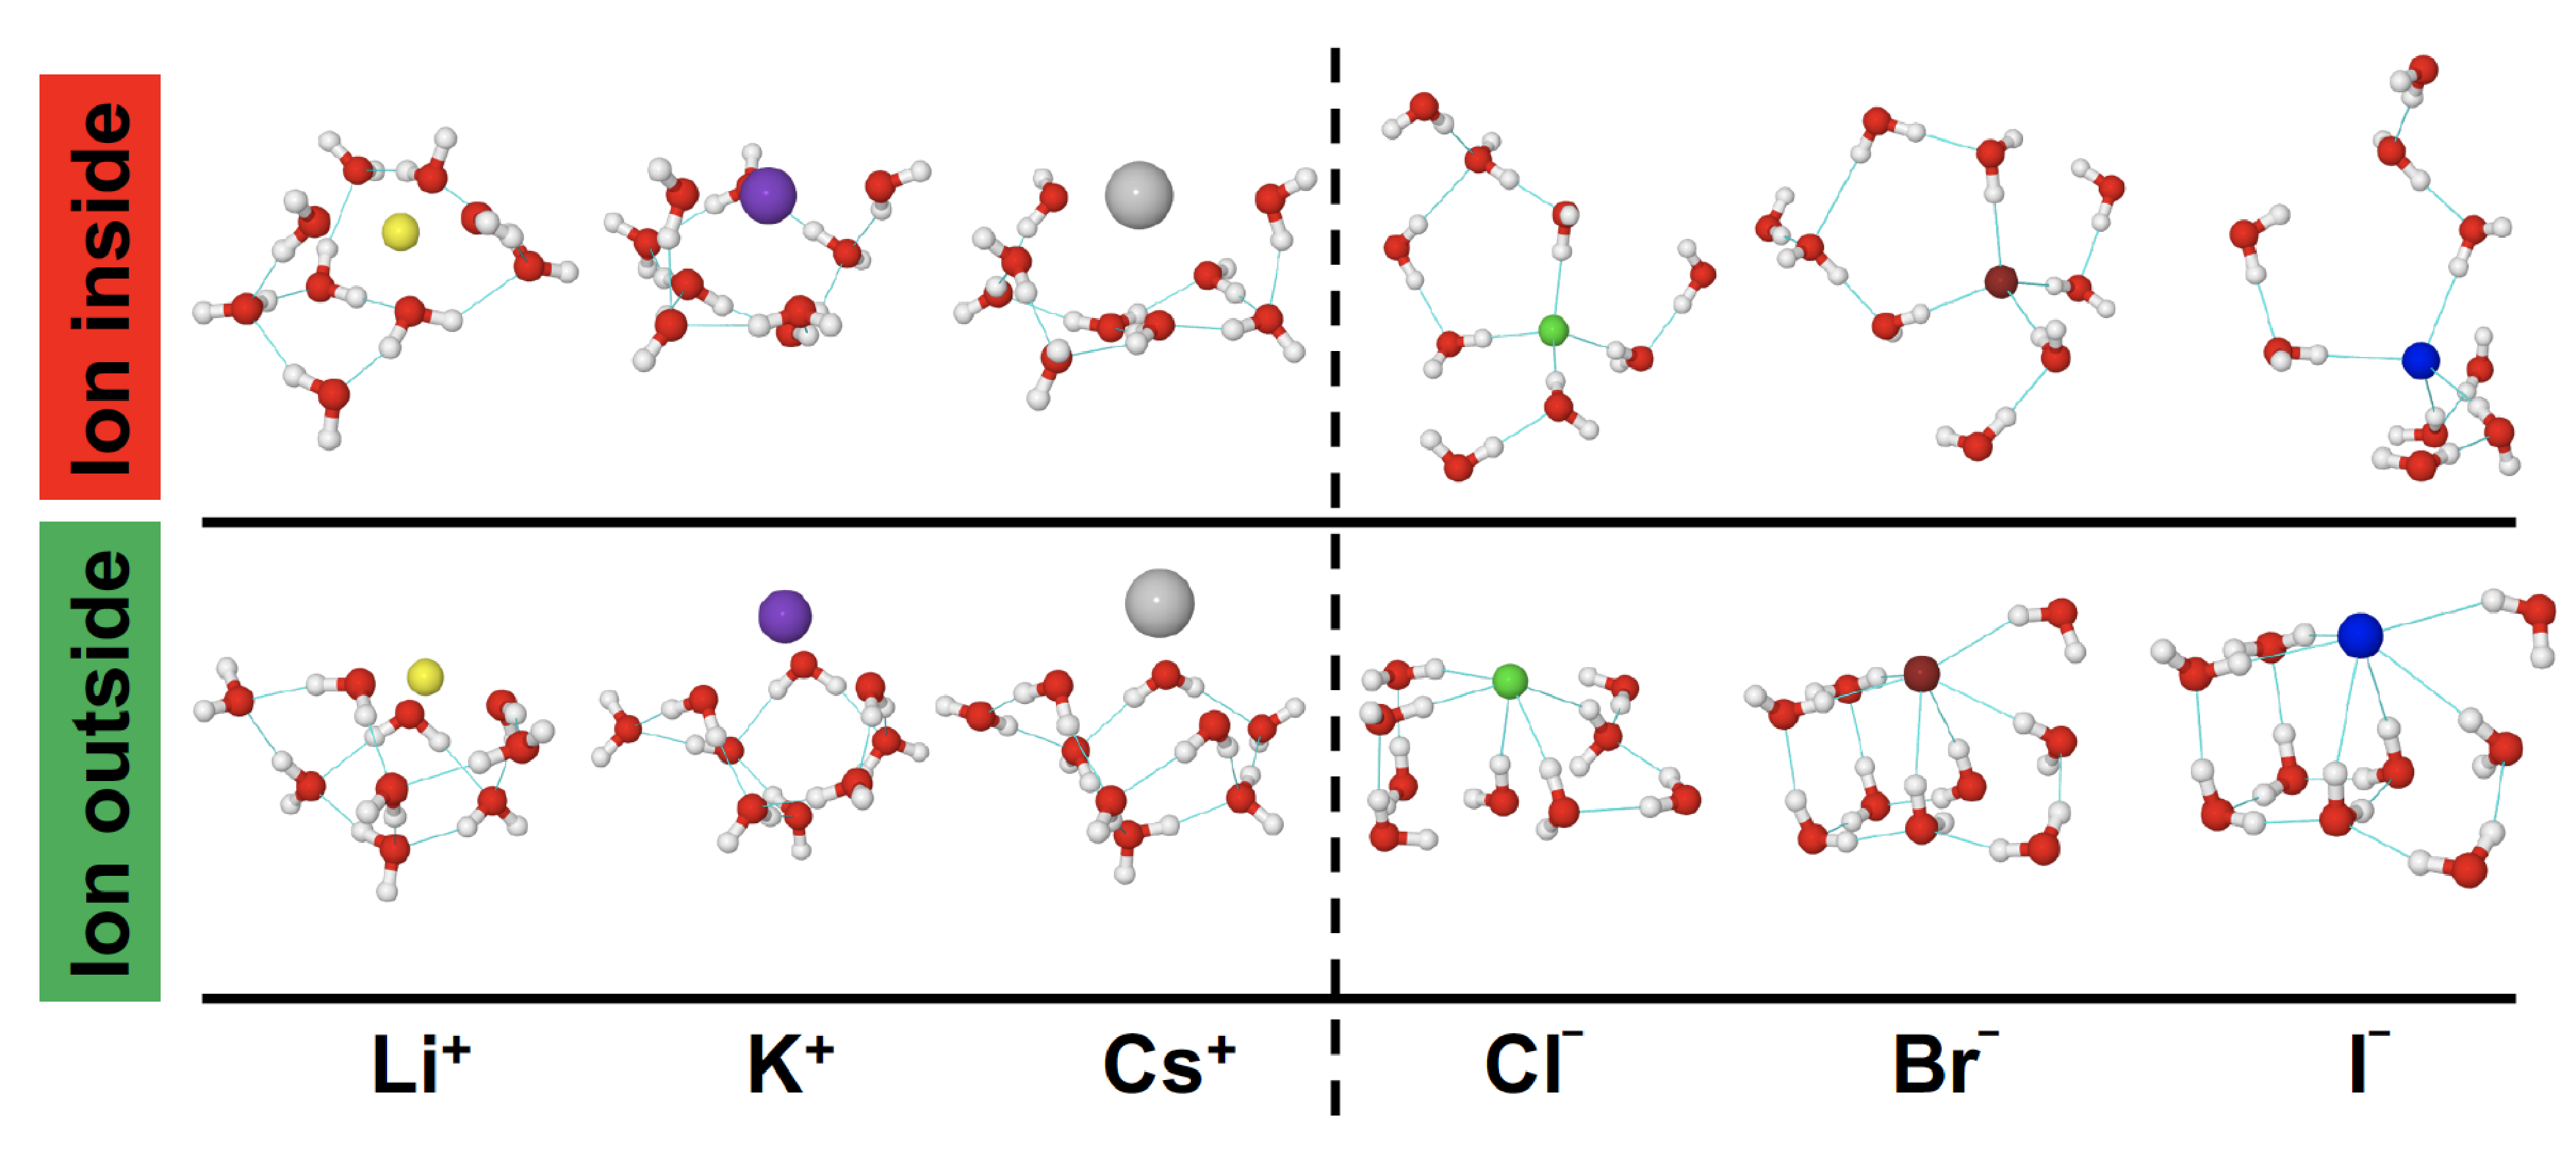
\includegraphics[width=\textwidth]{Figures/Chapter_3/figure_1.pdf}
\begin{spacing}{1.0}
\caption[Geometries of the ionic clusters used for the MBE calculation. For each ion, two different arrangements (ion inside, ion outside) were considered.]{Geometries of the ionic clusters used for the MBE calculation. For each ion, two different arrangements (ion inside, ion outside) were considered.}\label{fig:MBE_II_1}
\end{spacing}
\end{figure}
\begin{figure}[h]
\uwsinglespace
\centering
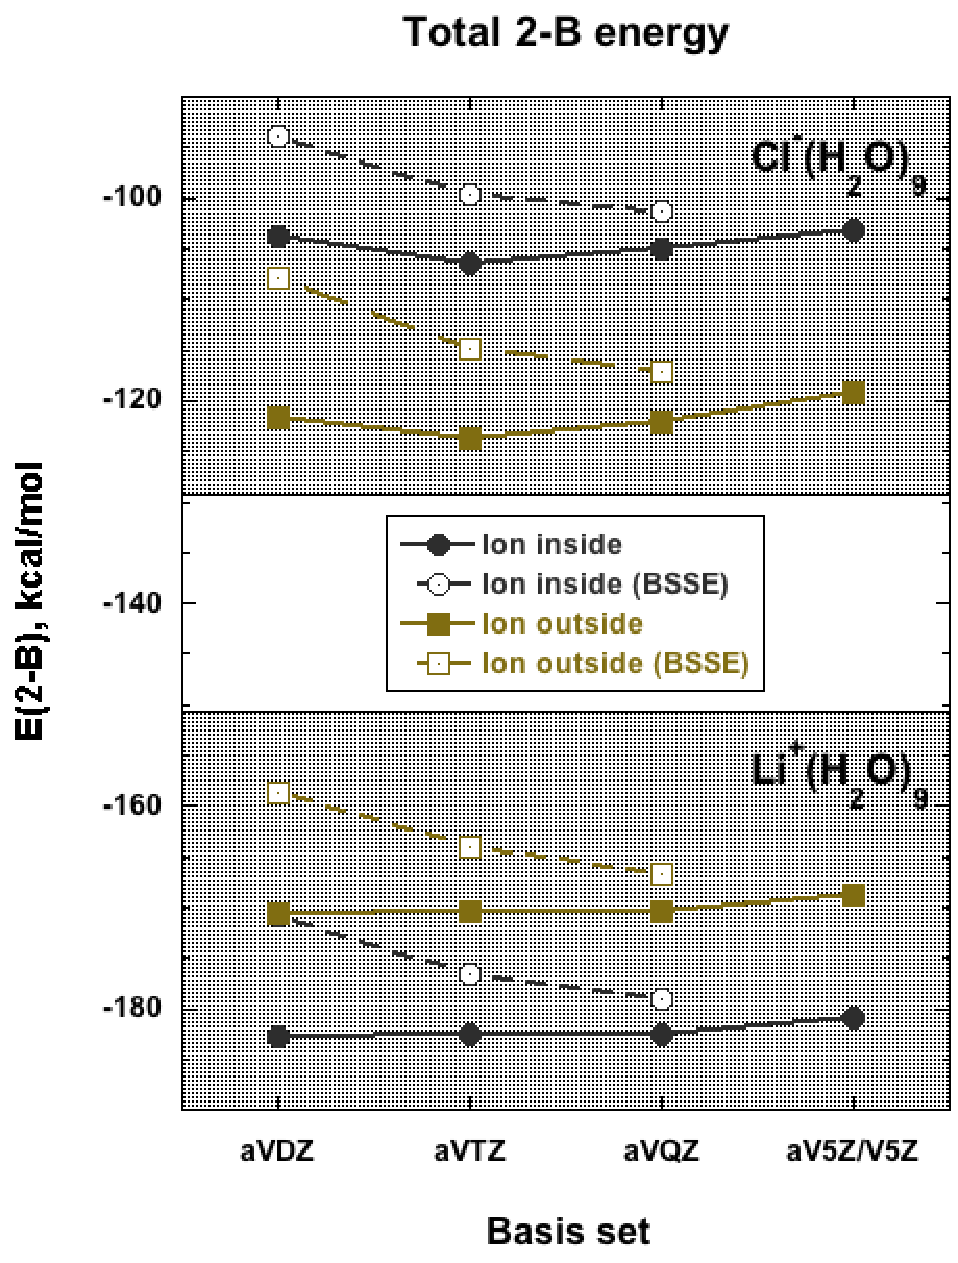
\includegraphics[width=.5\textwidth]{Figures/Chapter_3/figure_2.pdf}
\caption[Variation of the total uncorrected (filled symbols, solid lines) and BSSE-corrected (open symbols, dashed lines) 2-B energy with basis set for the ion inside and ion outside isomers of the \ce{Li^+(H2O)9} (lower shaded area) and \ce{Cl^-(H2O)9} (upper shaded area) clusters.]{Variation of the total uncorrected (filled symbols, solid lines) and BSSE-corrected (open symbols, dashed lines) 2-B energy with basis set for the ion inside and ion outside isomers of the \ce{Li^+(H2O)9} (lower shaded area) and \ce{Cl^-(H2O)9} (upper shaded area) clusters.}
\label{fig:MBE_II_2}
\end{figure}
\begin{figure}[h]
\uwsinglespace
\begin{center}
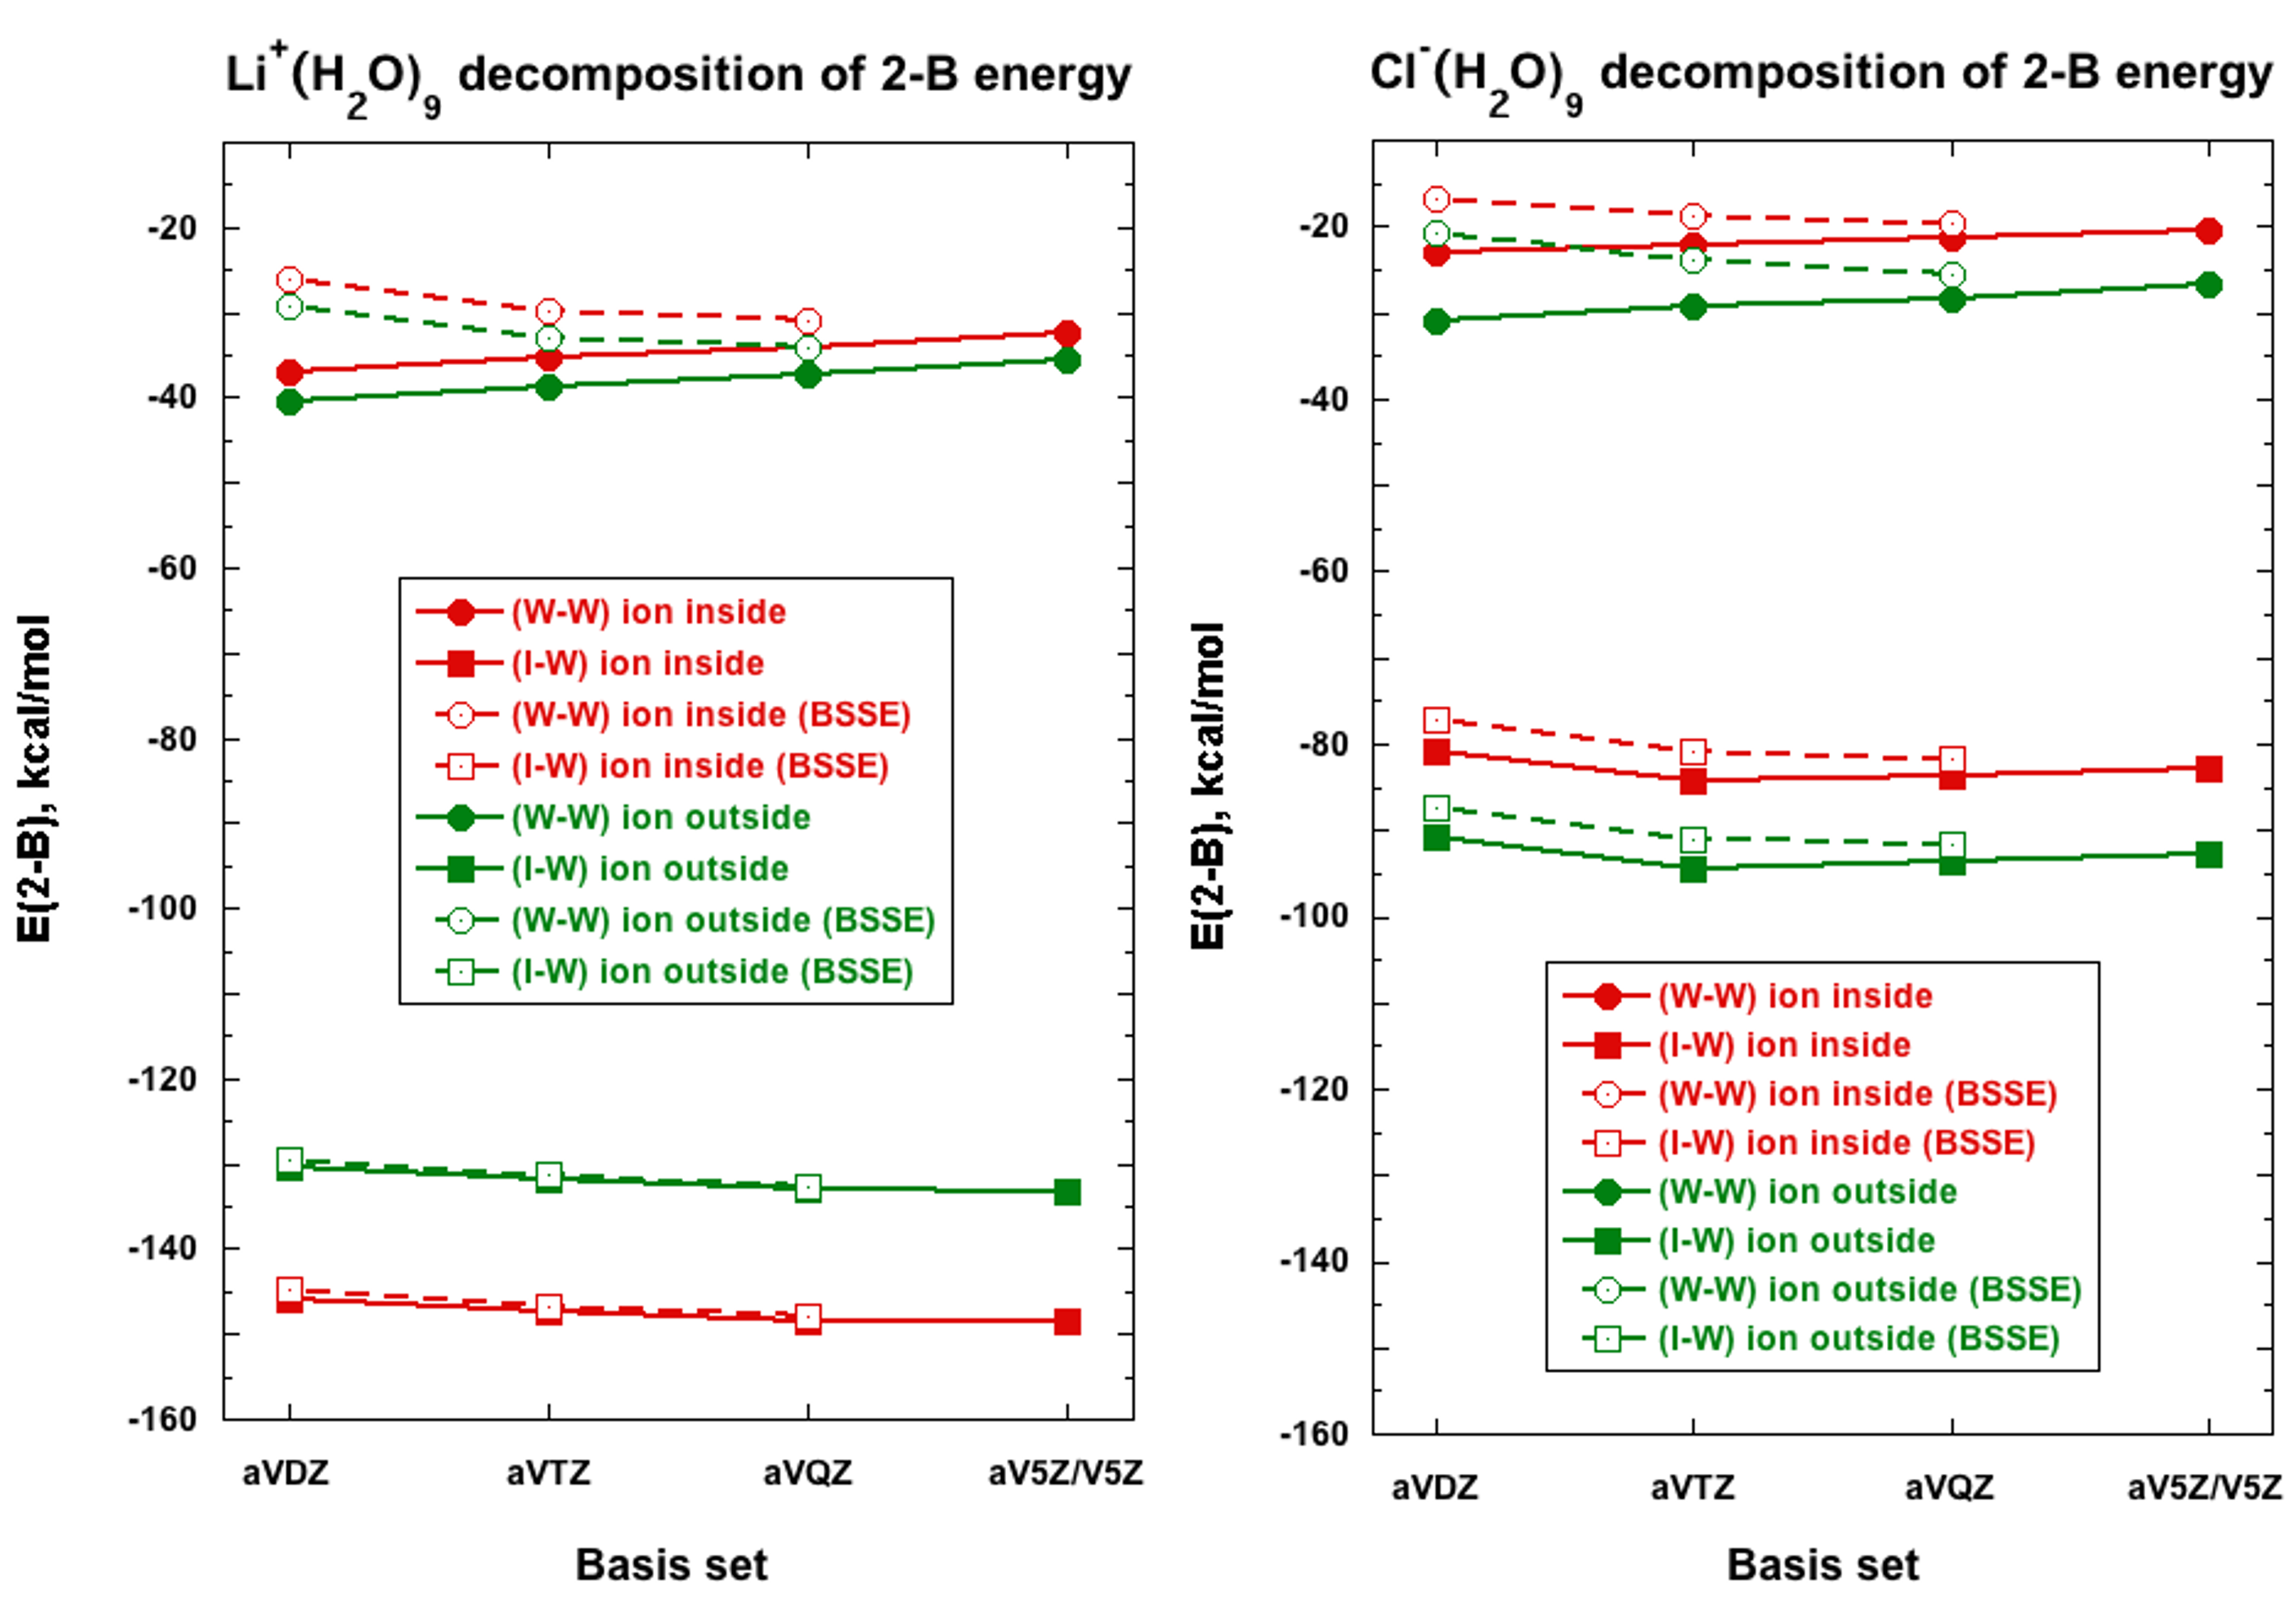
\includegraphics[width=\textwidth]{Figures/Chapter_3/figure_3_combined.png}
\end{center}
\caption[Magnitude of the individual ion-water (I-W) and water-water (W-W) 2-Body energy terms with (open symbols) and without (filled symbols) BSSE correction for the ion inside (red) and ion outside (green) configurations of the \ce{Li^+(H2O)9} (left panel) and \ce{Cl^-(H2O)9} (right panel) clusters. Notice the same y-axis scales.]{Magnitude of the individual ion-water (I-W) and water-water (W-W) 2-Body energy terms with (open symbols) and without (filled symbols) BSSE correction for the ion inside (red) and ion outside (green) configurations of the \ce{Li^+(H2O)9} (left panel) and \ce{Cl^-(H2O)9} (right panel) clusters. Notice the same y-axis scales.}
\label{fig:MBE_II_3}
\end{figure}

\par The difference in the magnitude of the (W-W) terms for each of the two ionic systems ($<$ 10 kcal/mol for both the ion inside and ion outside isomers) is indicative of the large effect which a cation has on disrupting hydrogen-bonding interactions amongst water molecules. This is because incorporating a cation into a hydrogen-bonding network requires a water molecule to interact via the oxygen as opposed to the hydrogen atom for the case of an anion. This is one of the reasons that the hydrogen bond lifetime depends more strongly on the cation identity while being almost indifferent to the identity of the anion, as was previously experimentally observed.\autocite{shalit_terahertz_2017}

\par In summary, the fact that the total 2-B interaction for \ce{Li^+(H2O)9} is larger than the one for \ce{Cl^-(H2O)9} has its origins in the stronger (I-W) interaction of the former compared to the latter. In addition, the relative ordering of the total 2-B interaction between the ion inside vs. ion outside configurations is mainly driven by the (I-W) interaction as the ordering of the (I-W) interaction is the same with the total 2-B for the two different arrangements. The stronger (I-W) interaction (\ce{Li^+}$...$\ce{H2O} compared to \ce{Cl^-}$...$\ce{H2O}) was found to correlate with a stronger (W-W) interaction as well.

\begin{figure}[t]
\uwsinglespace
\centering
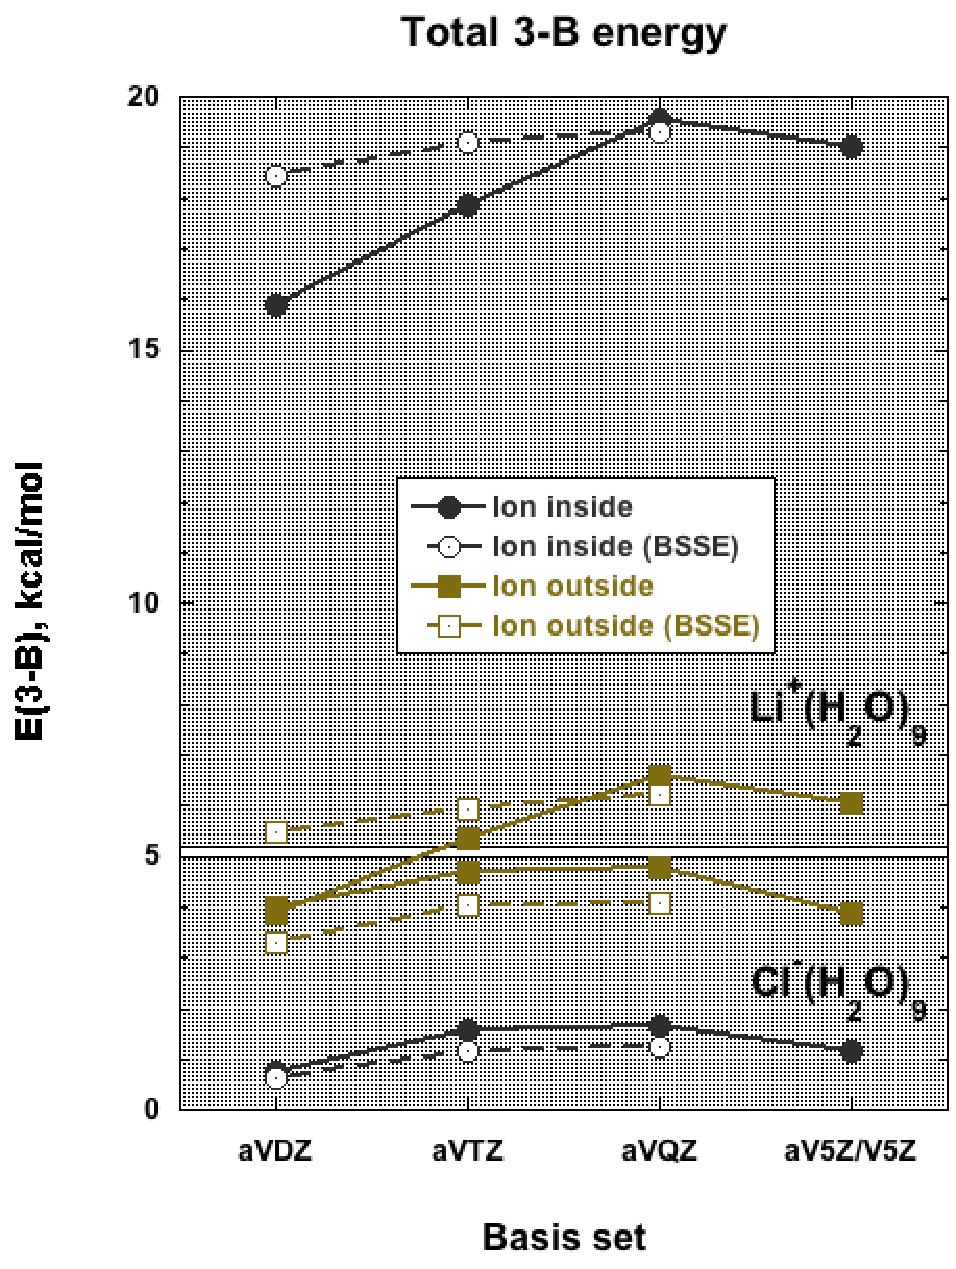
\includegraphics[width=.5\textwidth]{Figures/Chapter_3/figure_4.pdf}
\begin{spacing}{1.0}
\caption[Variation of the total uncorrected (filled symbols, solid lines) and BSSE-corrected (open symbols, dashed lines) 3-B energy with basis set for the ion inside and ion outside isomers of the \ce{Li^+(H2O)9} (upper shaded area) and \ce{Cl^-(H2O)9} (lower shaded area) clusters.]{Variation of the total uncorrected (filled symbols, solid lines) and BSSE-corrected (open symbols, dashed lines) 3-B energy with basis set for the ion inside and ion outside isomers of the \ce{Li^+(H2O)9} (upper shaded area) and \ce{Cl^-(H2O)9} (lower shaded area) clusters.}\label{fig:MBE_II_4}
\end{spacing}
\end{figure}

\textbf{3-B interaction (k = 3):} The variation of the total 3-B interaction with basis set is shown in Figure \ref{fig:MBE_II_4} for the two isomers of the \ce{Li^+(H2O)9} and \ce{Cl^-(H2O)9} clusters. The total 3-B terms are repulsive (destabilizing) for both ionic clusters and structural arrangements (Figure \ref{fig:MBE_II_4}). Note that for the 3-B term the BSSE correction does not always result in numbers that are lower than the uncorrected ones. The spread of the total 3-B energies for the two isomers of \ce{Li^+(H2O)9} (upper panel of Figure \ref{fig:MBE_II_4}) is much larger than the one found for the two isomers of the \ce{Cl^-(H2O)9} cluster (lower panel of Figure \ref{fig:MBE_II_4}); as in the case for the total 2-B interaction, the order of the total 3-B energies for the two structural arrangements is reversed between the two ionic clusters (more repulsive for the ion inside isomer of \ce{Li^+(H2O)9}, less repulsive for the same isomer of \ce{Cl^-(H2O)9}). Although the 3-B energies are in the 0-6 kcal/mol range for both isomers of \ce{Cl^-(H2O)9} and the ion outside isomer of \ce{Li^+(H2O)9}, we note a much larger (\textapprox20 kcal/mol) repulsive total 3-B energy for the ion inside isomer of the latter. This may suggest that both the strength and the total number of the (I-W) interactions influence the total 3-B energy. In Figure \ref{fig:MBE_II_5} we attempt to partition the total 3-B energies in terms of the individual (I-W-W) and (W-W-W) contributions for each ionic cluster. In the following we will assign the 3-B interactions as strong/weak based on a negative scale, i.e., a larger repulsive (destabilizing) interaction is described as “weaker” than a smaller repulsive (stabilizing) one, which is described as “stronger”. The two panels of Figure \ref{fig:MBE_II_5} are plotted with the same y-axis scale to make the comparison easier. For the ion inside isomer of the \ce{Li^+(H2O)9} cluster there exists a large (\textapprox25 kcal/mol) repulsive (I-W-W) interaction that is partially offset by a much smaller (\textapprox6 kcal/mol) attractive (W-W-W) interaction. Both of these interactions are smaller (\textapprox5 and \textapprox1 kcal/mol) and repulsive for the ion outside isomer of that cluster. In contrast, in the ion inside isomer of the \ce{Cl^-(H2O)9} cluster both components are quite small (\textless 2 kcal/mol) and repulsive, whereas for the ion outside isomer of this cluster they have opposite signs (the (W-W-W) interaction is attractive) and almost cancel each other. 

\begin{figure}[h]
\uwsinglespace
\begin{center}
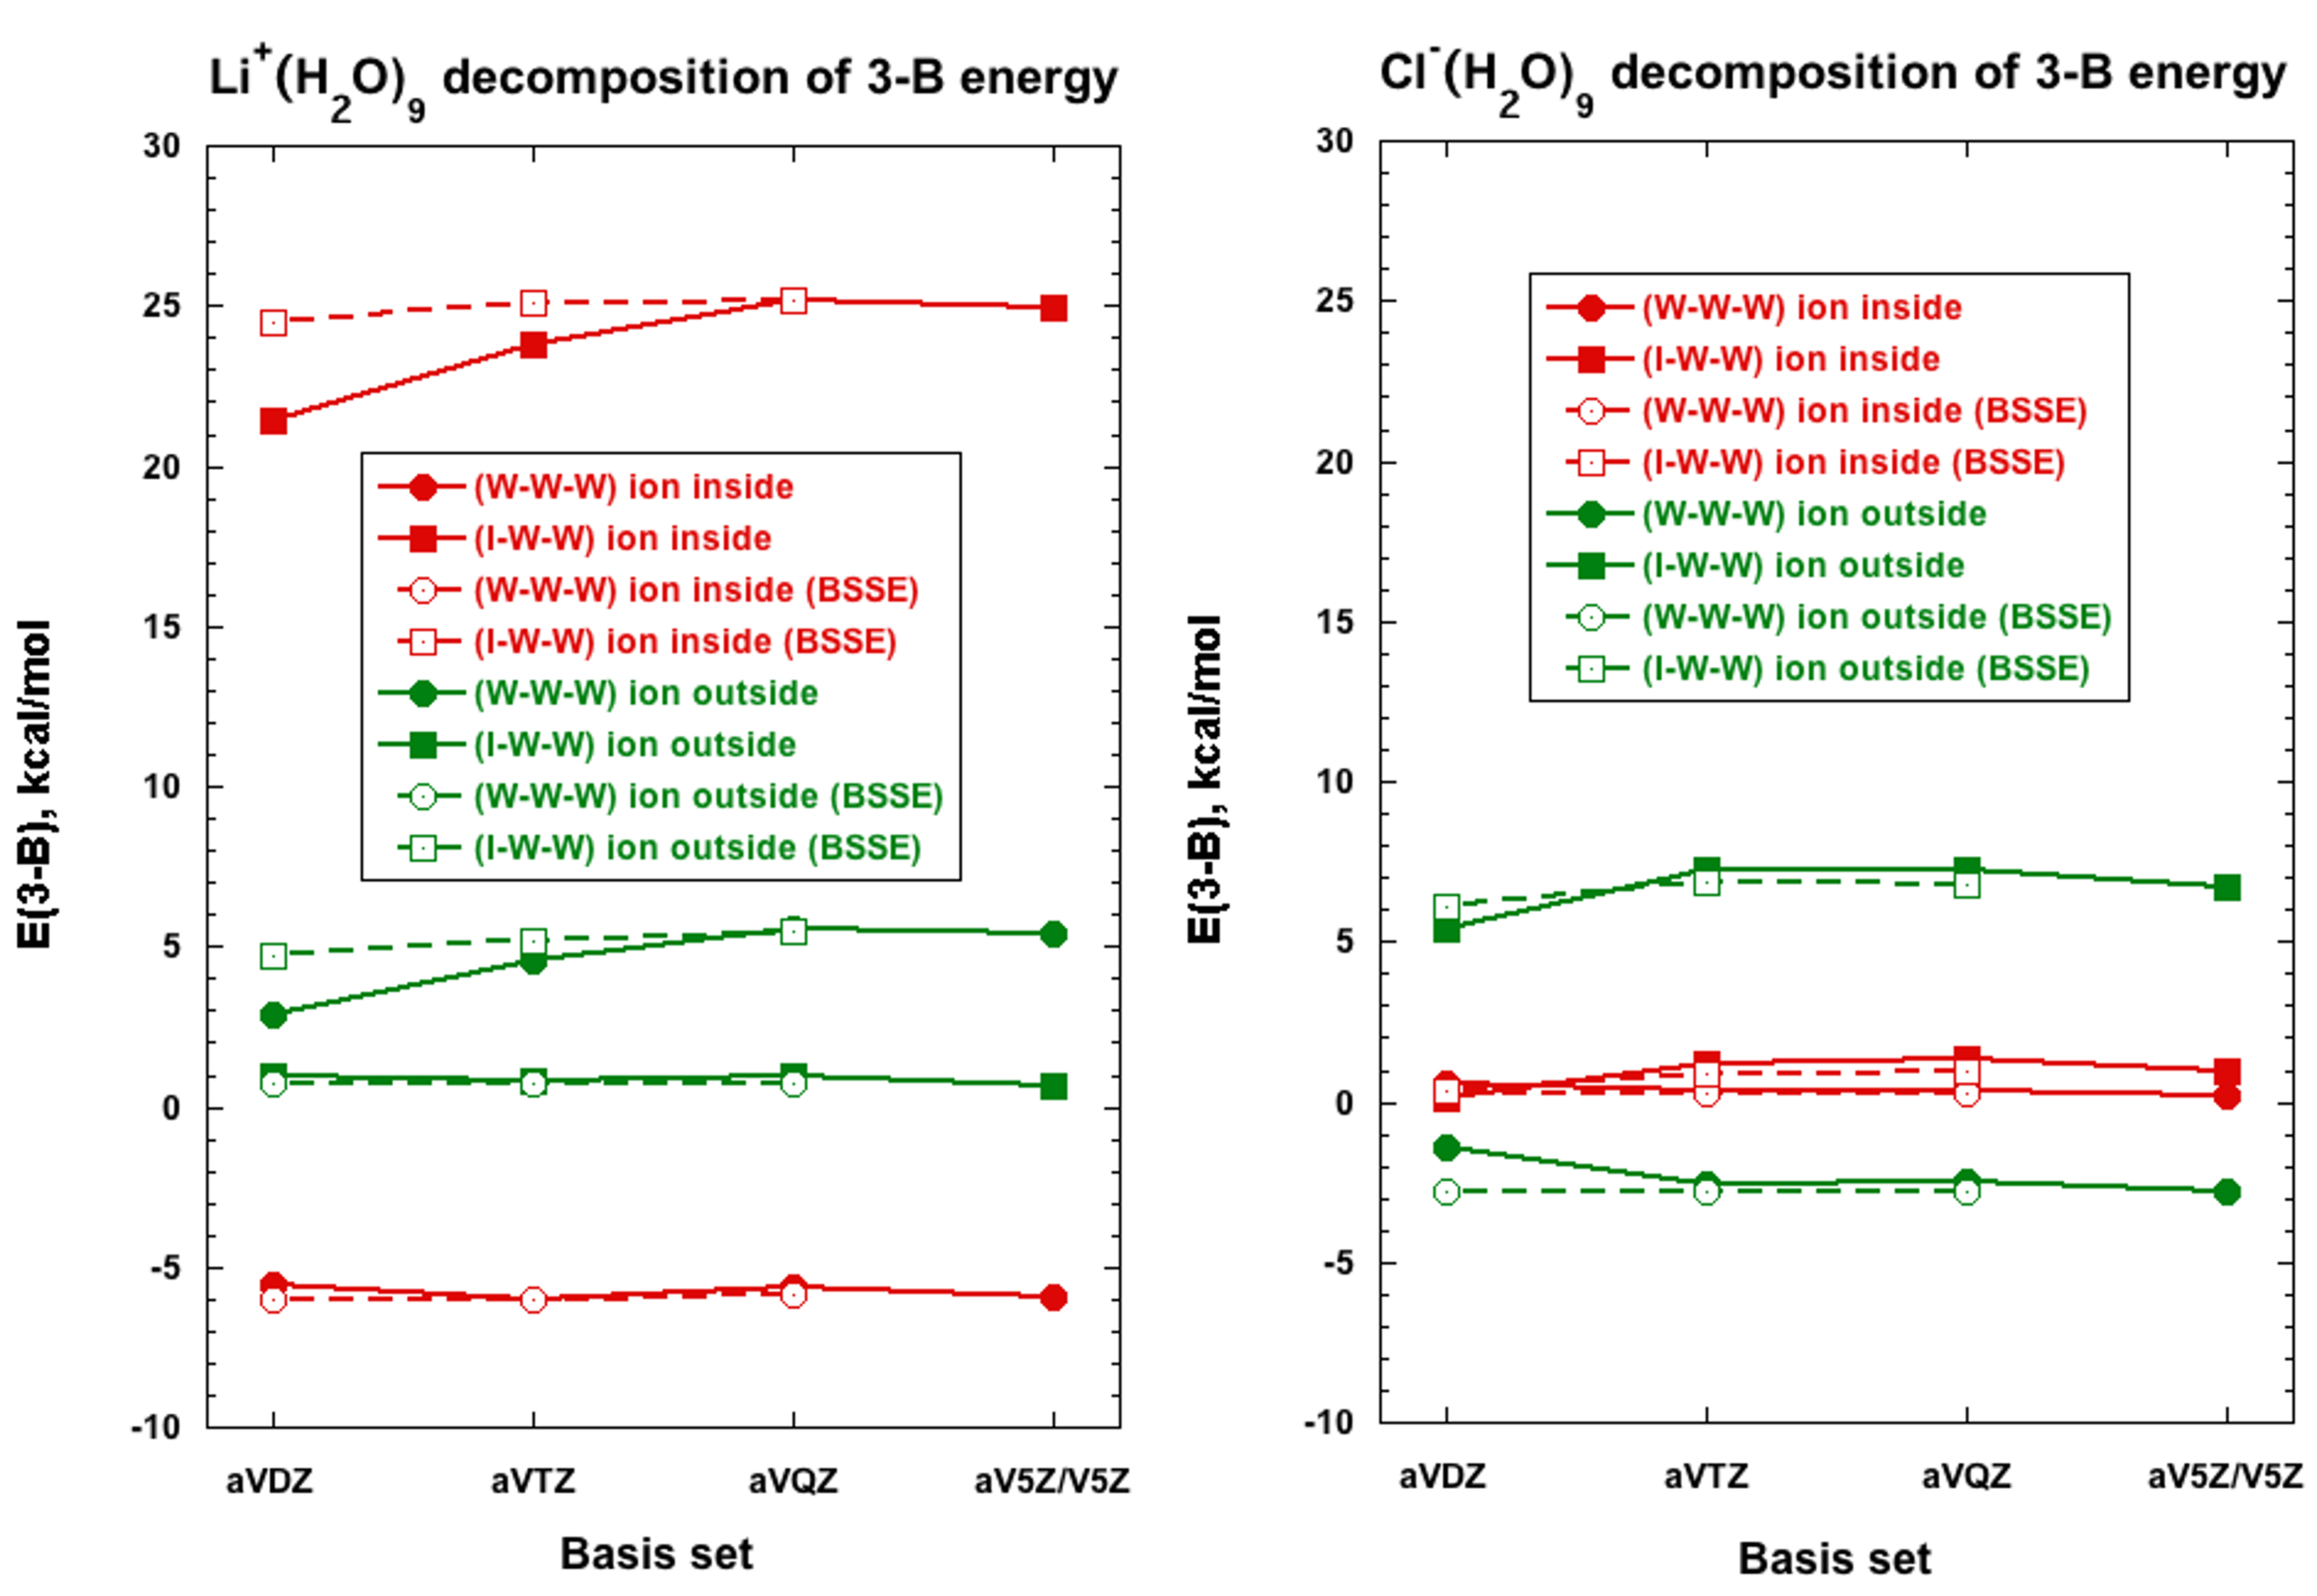
\includegraphics[width=\textwidth]{Figures/Chapter_3/figure_5_combined.png}
\end{center}
\caption[Magnitude of the 3-Body energy with and without BSSE correction for \ce{Cl^-(H2O)9} (left) and \ce{Li^+(H2O)9} (right) split into contributions from ion-water-water interactions and water-water-water interactions. Notice the same y-axis scales.]{Magnitude of the 3-Body energy with and without BSSE correction for \ce{Cl^-(H2O)9} (left) and \ce{Li^+(H2O)9} (right) split into contributions from ion-water-water interactions and water-water-water interactions. Notice the same y-axis scales.}
\label{fig:MBE_II_5}
\end{figure}

\par From the limited sampling of configurational space examined here (i.e., just two conformations with the ion inside and outside a water network) we are not able to arrive at general conclusions regarding the sign and magnitude of the 3-B (I-W-W) and (W-W-W) terms based on either the strength or the number (coordination) of the (I-W) interactions. Indeed, when comparing \ce{Li^+} vs. \ce{Cl^-}, a stronger (I-W) interaction (Li+) is associated with a weaker (I-W-W) and a stronger (W-W-W) interaction for the ion inside isomer, but the situation is reversed for the ion outside isomer which has a stronger (I-W-W) and a weaker (W-W-W) interaction. This is also easily seen by the relative positions of the red (ion inside isomer) and green lines (ion outside isomer) in the two panels of Figure \ref{fig:MBE_II_5}: the green lines lie in between the red ones in the left panel, while the situation is reversed (red lines in between the green ones) in the right panel. That is, for the inside isomers, where the number of (I-W) bonds is larger, \ce{Li^+} results in weaker (I-W-W) and stronger (W-W-W) interactions, whereas the situation is reversed for \ce{Cl^-}.

\par It is worth noting that the two most repulsive total (I-W-W) terms for the ion inside isomer of \ce{Li^+(H2O)9} (left panel of Figure \ref{fig:MBE_II_5}) and ion outside isomer of \ce{Cl^-(H2O)9} (right panel of Figure \ref{fig:MBE_II_5}) correspond to the cases associated with the most stabilizing total (W-W-W) interactions. While we cannot make definitive generalizations from the limited sampling of configurations studied here, this may indicate a type of anti-cooperative effect between the ion-water interactions and the water-only hydrogen bonding networks. This follows from the fact that the 3-body term is a sensitive measure of the degree of cooperativity in aqueous clusters.\autocite{xantheas_cooperativity_2000} The fact that the ion-water interactions weaken the ability of water to hydrogen-bond cooperatively\autocite{xantheas_cooperativity_2000} is also evident from the fact that the (W-W-W) terms are barely stabilizing or essentially zero for both cases. These terms are much smaller in magnitude and as a percentage of the total binding energy (vide infra) than the corresponding ones previously found for pure water clusters.\autocite{heindel_many-body_2020}

\par Another interesting point is that the (I-W-W) interactions are destabilizing by about 25 kcal/mol when \ce{Li^+} resides on the inside of the water cluster. On the other hand, the (I-W) interactions are more strongly stabilizing for the inside isomer of \ce{Li^+(H2O)9}. These observations reinforce the idea that cations tend to disrupt the hydrogen-bonding network in water so that water has a difficult time favorably interacting with itself. Therefore, the relatively large role of many-body terms for a cation compared to an anion is perhaps counter-intuitive when we tend to associate many-body effects with induction and polarizability,\autocite{heindel_origin_2018,zhuang_many-body_2019} which one would also expect to be larger in anionic systems.

\par In terms of the trends observed in Figure \ref{fig:MBE_II_4}, the magnitude of the total 3-B term is mainly determined by the (I-W-W) interaction. This interaction is substantial for the ion inside arrangement of the \ce{Li^+(H2O)9} cluster but quite small for its outside arrangement as well as for both arrangements of the \ce{Cl^-(H2O)9} cluster. The above findings justify the previous use of an (I-W-W) 3-B exchange potential for the modeling of the solvation of strongly bound ions (\ce{Li^+} and \ce{F^-}) in water, i.e. arrangements that the ion is fully solvated,\autocite{dang_ion_1991,xantheas_critical_1996} whereas the inclusion of this additional interaction did not seem to make a difference for the solvation of \ce{Cl^-} ions in water.\autocite{perera_structures_1994}

\textbf{4-B interaction (k = 4):} The importance of M-B terms beyond the 3-B for aqueous systems was somewhat unclear for a while, but recently a consensus has been reached that including the 4-body term is quite important if one is interested in accuracies on the order of 1 kcal/mol.\autocite{heindel_benchmark_2018,lao_understanding_2016,richard_aiming_2014,howard_n-body_2013} This raises the question whether the MBE actually converges smoothly, or if terms beyond the 4-B are also necessary. In our first paper of this series,\autocite{heindel_many-body_2020} we have conclusively shown that terms beyond the 4-body are practically negligible in calculations of the binding energy of neutral water clusters, which agrees with similar calculations done previously at the Hartree-Fock level.\autocite{ouyang_trouble_2014,ouyang_many-body_2015} This statement comes with the caveat that one includes a proper correction for BSSE, which will otherwise cause the 5-body and higher-order terms to erroneously appear to be large and oscillating in magnitude around zero.

\begin{figure}[t]
\uwsinglespace
\centering
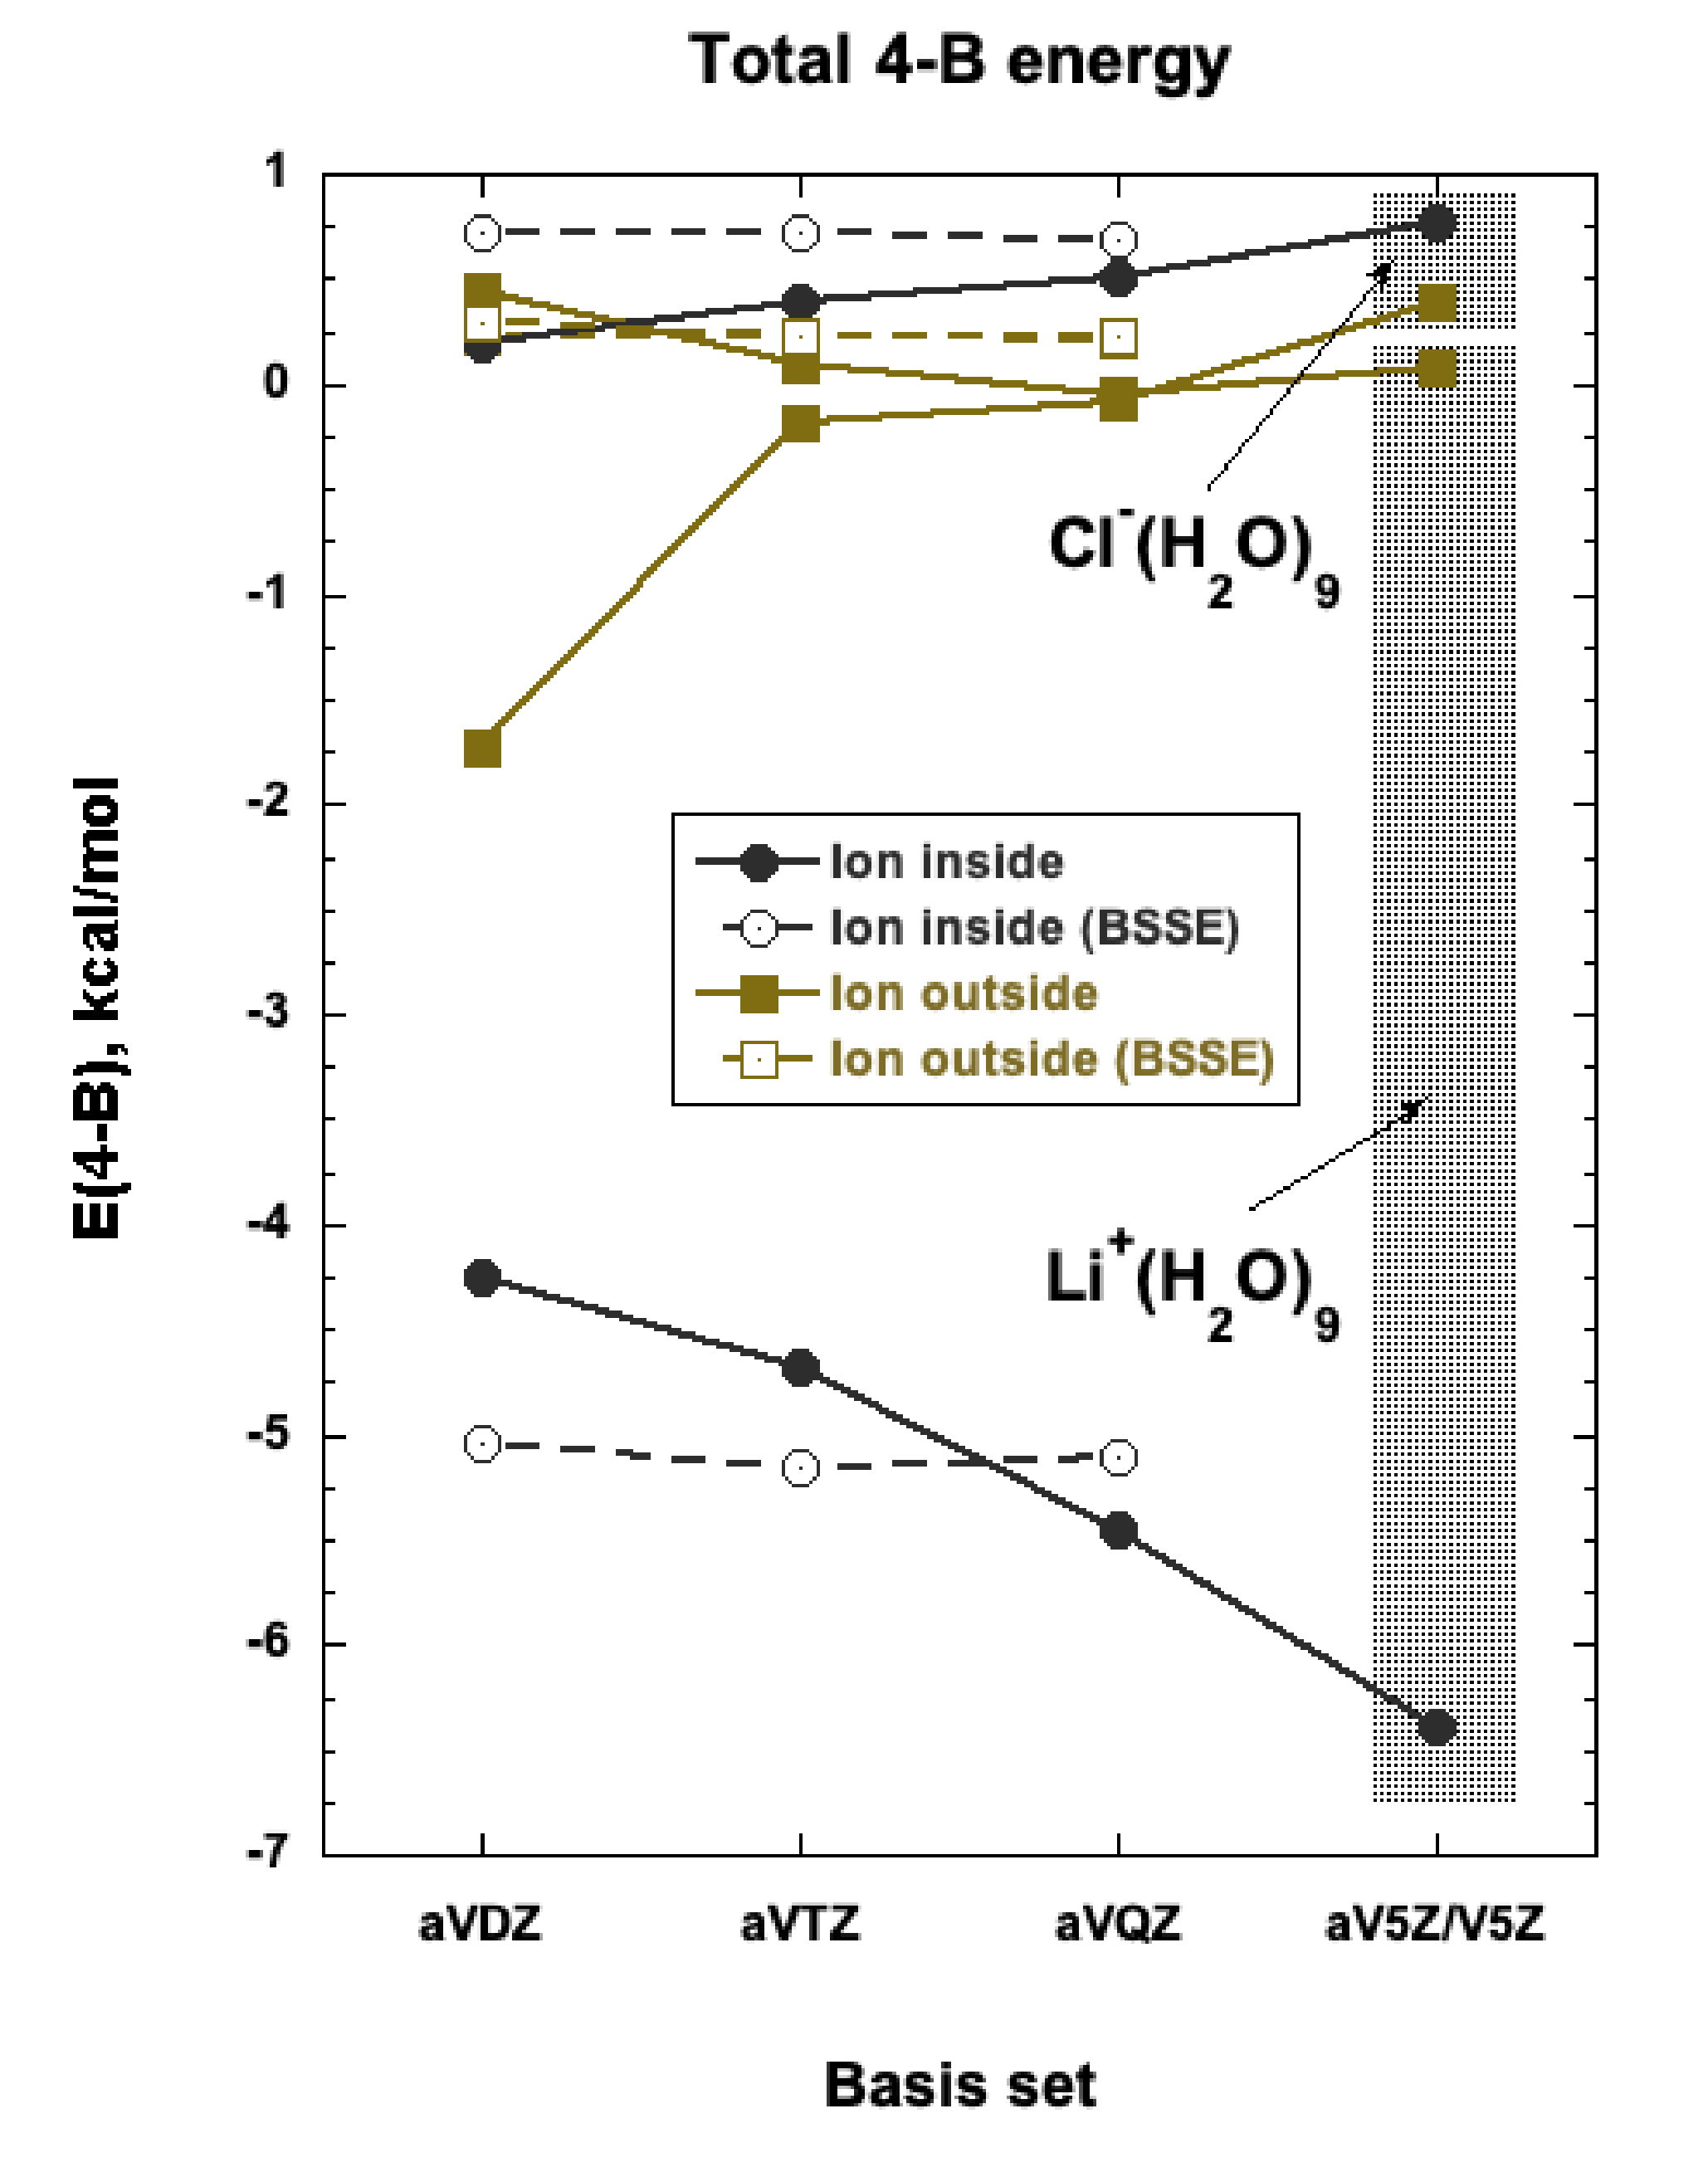
\includegraphics[width=.5\textwidth]{Figures/Chapter_3/figure_6.pdf}
\begin{spacing}{1.0}
\caption[Variation of the total uncorrected (filled symbols, solid lines) and BSSE-corrected (open symbols, dashed lines) 4-B energy with basis set for the ion inside and ion outside isomers of the \ce{Li^+(H2O)9} (lower shaded area) and \ce{Cl^-(H2O)9} (upper shaded area) clusters.]{Variation of the total uncorrected (filled symbols, solid lines) and BSSE-corrected (open symbols, dashed lines) 4-B energy with basis set for the ion inside and ion outside isomers of the \ce{Li^+(H2O)9} (lower shaded area) and \ce{Cl^-(H2O)9} (upper shaded area) clusters.}\label{fig:MBE_II_6}
\end{spacing}
\end{figure}

\par Figure \ref{fig:MBE_II_6} shows the variation of the total 4-B interaction with basis set for the two isomers of the \ce{Li^+(H2O)9} and \ce{Cl^-(H2O)9} clusters. The interaction is practically zero except for the ion inside isomer of the \ce{Li^+(H2O)9} cluster, for which the main contribution (\textgreater 95\% at the aVQZ, BSSE corrected) comes from the (I-W-W-W) interaction. These results suggest that the 4-B term can be safely omitted when modeling the various arrangements of the ion in the Cl-(H2O)9 cluster and structures in which the \ce{Li^+} ion resides on the surface of a water cluster; however, this will result in an error of \textapprox5\% for configurations where the \ce{Li^+} ion is fully solvated by a water network.
\begin{figure}[H]
    \centering
    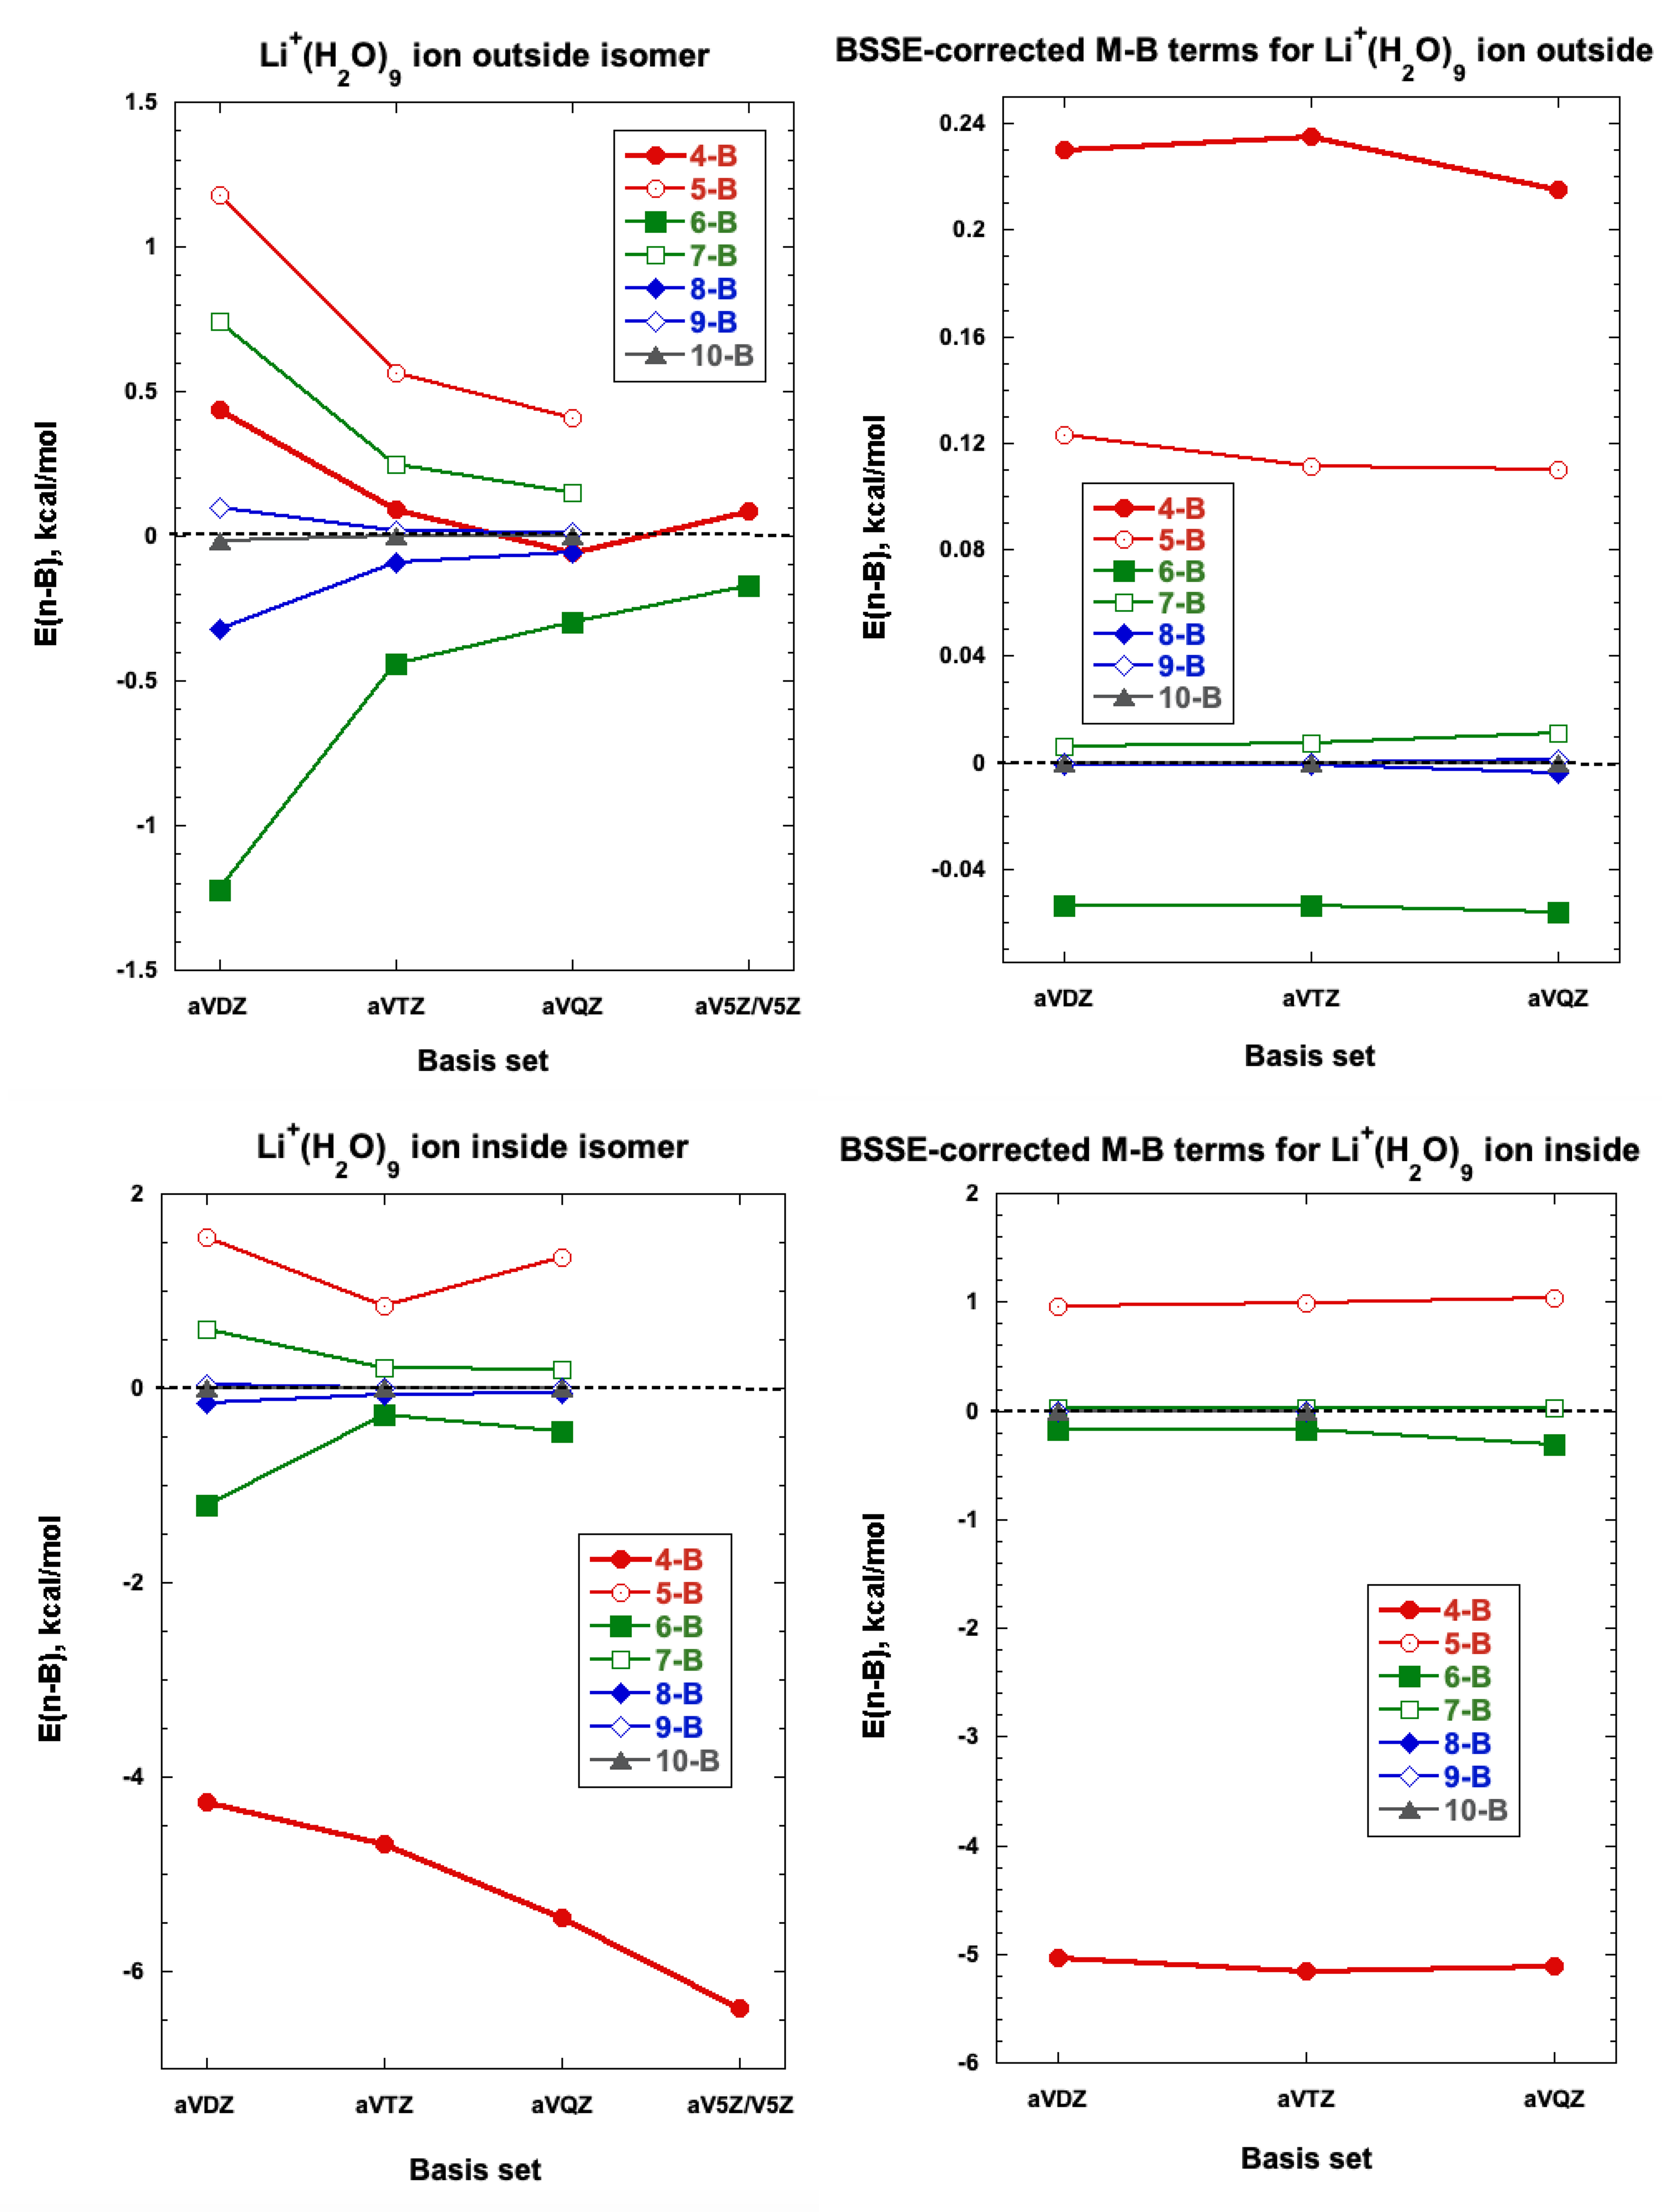
\includegraphics[width=.9\textwidth]{Figures/Chapter_3/figure_6_combined.png}
  \caption{Many-body terms for \ce{Li^+(H2O)9}. Notice the different y-axis scales.}
  \label{fig:MBE_II_7}
\end{figure}

\textbf{Higher order interactions (k = 5 – 10):} The variation of the 4- through 10-body terms with basis set for the ion outside and ion inside isomers is shown in Figure \ref{fig:MBE_II_7} for the \ce{Li^+(H2O)9} and Figure \ref{fig:MBE_II_8} for the \ce{Cl^-(H2O)9} clusters, respectively. In each Figure there are 4 panels, two for the ion outside (top) and two for the ion inside (bottom). The left panels (top, bottom) trace the uncorrected, while the right panels (top, bottom) the BSSE corrected numbers.

\par In general, we observe a pattern in the variation of the higher order ($k \geq 5$) MBE terms with basis set that is similar to the one observed earlier for pure water clusters,\autocite{heindel_many-body_2020} namely an undulation around zero for the even and odd MBE terms and their convergence to practically zero with the larger basis set used in this study (aV5Z/V5Z). All BSSE-corrected MB terms ($k \geq 4$) are practically constant with basis set size, a result similar to the one previously found for pure water clusters.\autocite{heindel_many-body_2020} However, the convergence of the BSSE-uncorrected 4-B term is in some instances not monotonic with basis set. For example, the BSSE uncorrected 4-B term for the outside isomers of both ions (top left panels in Figures \ref{fig:MBE_II_7} and \ref{fig:MBE_II_8}) switches from a small negative to a small positive value going from the aVQZ to the aV5Z/V5Z basis set. This change in sign is real as confirmed from the positive BSSE-corrected values of the 4-B term for these isomers (top right panels in Figures \ref{fig:MBE_II_7} and \ref{fig:MBE_II_8}). Therefore, the conclusion that the calculation of the 4-B (and higher) terms with just the aVDZ basis set including BSSE corrections produces aV5Z (or close to CBS) quality values, previously observed for pure water clusters,\autocite{heindel_many-body_2020} is also valid for the ionic aqueous clusters considered in this study.
\begin{figure}[H]
    \centering
    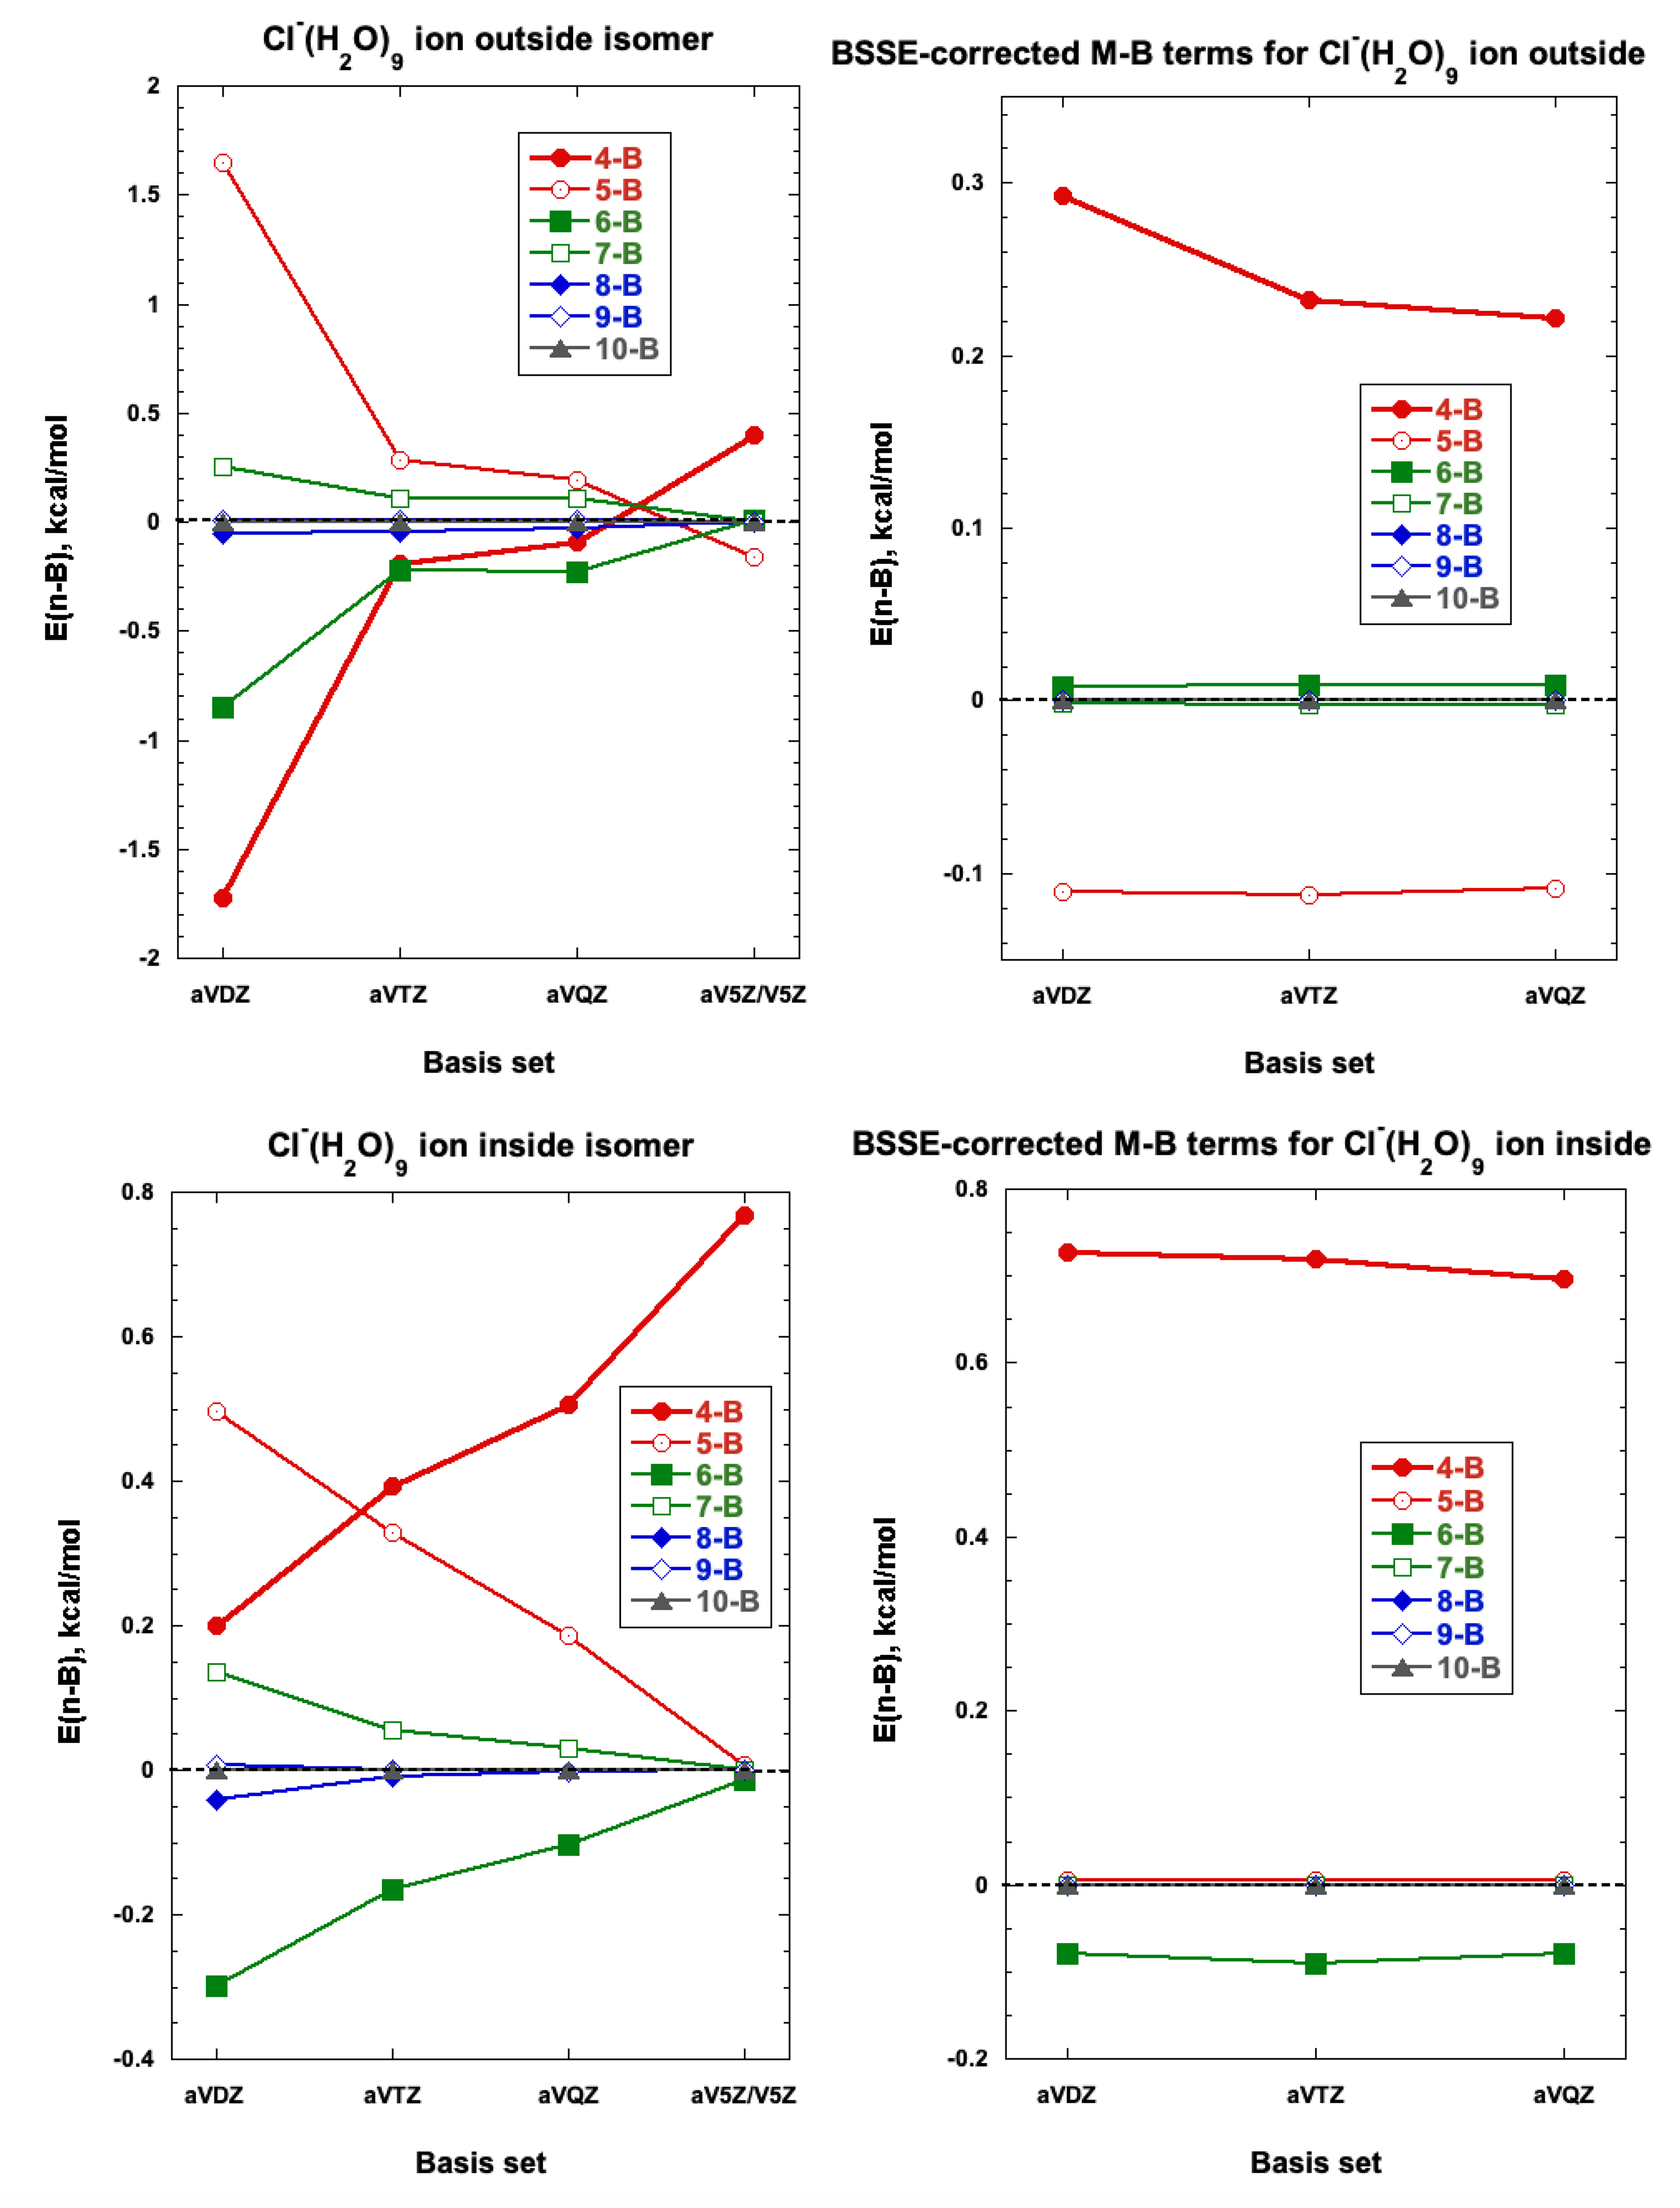
\includegraphics[width=.9\textwidth]{Figures/Chapter_3/figure_8_combined.png}
  \caption[Many-body terms for \ce{Cl^-(H2O)9}.]{Many-body terms for \ce{Cl^-(H2O)9}. Notice the different y-axis scales.}
  \label{fig:MBE_II_8}
\end{figure}

\subsection{Many body terms of \ce{Z^{+/-}(H2O)9} (\ce{Z} = \ce{Li}, \ce{K}, \ce{Cs}, \ce{Cl}, \ce{Br}, \ce{I}):}

\par The discussion in the previous sections suggests that the BSSE-corrected MP2/aVDZ results for the $k \geq 3$ M-B terms provide accurate estimates of their values with larger basis sets and/or at the CBS limit. For this reason, we carried out the MBE up to $k = 5$ for the remaining \ce{Z^{+/-}(H2O)9} clusters, \ce{Z} = \ce{K^+}, \ce{Cs^+}, \ce{Br^-}, \ce{I^-}, at the MP2/aVDZ level including corrections for BSSE. Selected results are listed in Table \ref{tab:MBE_II_T2}. The results for the \ce{Li^+(H2O)9} and \ce{Cl^-(H2O)9} at this level of theory are also included for completeness. These are not to be confused with the ones contained in Table \ref{tab:MBE_II_1} at the MP2/aVQZ level of theory for these two clusters. We will rely on this data to identify correlations between the ion-water and water-water terms in the next section.

\begin{table}[t]
\begin{adjustbox}{width=\columnwidth,center}
\begin{tabular}{@{}llllll@{}}
\toprule
\textbf{M-B term} & \multicolumn{2}{c}{\ce{Li^+(H2O)9}}     & \multicolumn{2}{c}{\ce{Cl^-(H2O)9}}     & \ce{(H2O)_{10}}       \\ \hline
                  & Ion outside     & Ion inside      & Ion outside     & Ion inside      &               \\ \hline
Total 1-B         & 1.49 (-0.9)     & 2.30 (-1.4)     & 1.91 (-1.7)     & 1.76 (-1.8)     & 4.45 (-4.9)   \\ \hline
Total 2-B         & -166.78 (105.0) & -178.98 (110.7) & -117.14 (105.5) & -101.32 (103.8) & -72.39 (79.2) \\
(I-W)             & -132.57 (83.5)  & -147.92 (91.5)  & -91.66 (82.5)   & -81.58 (83.6)   & -             \\
(W-W)             & -34.21 (21.5)   & -31.06 (19.2)   & -25.48 (22.9)   & -19.73 (20.2)   & -             \\ \hline
Total 3-B         & 6.21 (-3.9)     & 19.29 (-11.9)   & 4.07 (-3.7)     & 1.23 (-1.3)     & -21.58 (23.6) \\
(I-W-W)           & 5.50 (-3.5)     & 25.18 (-15.6)   & 6.82 (-6.1)     & 0.98 (-1.0)     & -             \\
(W-W-W)           & 0.70 (-0.4)     & -5.89 (3.6)     & -2.75 (2.5)     & 0.25 (-0.3)     & -             \\ \hline
Total 4-B         & 0.22 (-0.1)     & -5.11 (3.2)     & 0.22 (-0.2)     & 0.70 (-0.7)     & -1.92 (2.1)   \\
(I-W-W-W)         & 0.20 (-0.1)     & -4.88 (3.0)     & 0.27 (-0.2)     & 0.55 (-0.6)     & -             \\
(W-W-W-W)         & 0.02 (0.0)      & -0.24 (0.2)     & -0.04 (0.0)     & 0.15 (-0.1)     & -             \\ \hline
Total 5-B         & 0.11 (-0.1)     & 1.03 (-0.6)     & -0.11 (0.1)     & 0.01 (0.0)      & 0.01 (0.0)    \\
(I-W-W-W-W)       & 0.12 (-0.1)     & 1.02 (-0.6)     & -0.14 (0.1)     & 0.01 (0.0)      & -             \\
(W-W-W-W-W)       & -0.01 (0.0)     & -0.01 (0.0)     & 0.03 (0.0)      & -0.002 (0.0)    & -             \\ \hline
Sum 6-B to 10-B   & -0.05 (0.0)     & -0.21 (0.1)     & 0.01 (0.0)      & -0.01 (0.0)     & 0.04 (0.0)    \\ \hline
Total De          & -158.81         & -161.67         & -111.04         & -97.64          & -91.39       \\ \bottomrule
\end{tabular}
\end{adjustbox}
\begin{spacing}{1.0}
\caption[Magnitude of the many-body terms for the two isomers of the \ce{Li^+(H2O)9} and \ce{Cl^-(H2O)9} clusters at the MP2/AVQZ level including BSSE-corrections. Bold numbers indicate the total energy of each term in kcal/mol with the percentage of the binding energy given in parentheses. Each term is further split into water-only and ion-water contributions. Results for \ce{(H2O)_{10}} from the MBE-I paper are given for reference to a neutral water system.]{Magnitude of the many-body terms for the two isomers of the \ce{Li^+(H2O)9} and \ce{Cl^-(H2O)9} clusters at the MP2/AVQZ level including BSSE-corrections. Bold numbers indicate the total energy of each term in kcal/mol with the percentage of the binding energy given in parentheses. Each term is further split into water-only and ion-water contributions. Results for \ce{(H2O)_{10}} from the MBE-I paper are given for reference to a neutral water system.}\label{tab:MBE_II_1}
\end{spacing}
\end{table}

\par It is also of interest to investigate the contributions to the MB terms originating from the Hartree-Fock (HF) and the electron correlation as it was previously done for the water clusters.\autocite{heindel_many-body_2020} Since the MBE equations only involve sums over energies, each term in the MBE can be cast as the sum $E_{MP2}=E_{HF}+E_{corr}$. Therefore, each $k$-body term can be split into two separate contributions arising from the HF and the correlation energy. The contribution of the correlation energy to the various many-body terms of the \ce{Z^{+/-}(H2O)9} clusters, \ce{Z} = \ce{K^+}, \ce{Cs^+}, \ce{Br^-}, \ce{I^-}, is listed in Table \ref{tab:MBE_II_3}. This analysis is the same and produces similar results with the one reported earlier for water clusters, suggesting that by neglecting the correlation contribution in all terms above the 3-body results in maximum error of (0.6\%) and in most instances in a much smaller error (\textless 0.1\%).

\begin{table}[t]
\begin{adjustbox}{width=\columnwidth,center}
\begin{tabular}{@{}ccccccccc@{}}
\toprule
\multicolumn{2}{l}{\textbf{Cluster}} & \textbf{Binding Energy} & \textbf{Total 2-B} & \textbf{I-W}     & \textbf{W-W}    & \textbf{Total 3-B} & \textbf{I-W-W} & \textbf{W-W-W}  \\ \hline
                  & \multicolumn{8}{c}{\textbf{\ce{Li^+(H2O)9}}}                                                                                                                                                                                        \\ \hline
\multicolumn{2}{l}{Ion inside}       & -154.44        & -170.78                                                                & -144.68 & -26.10 & 18.46                                                               & 24.46 & -6.00  \\
\multicolumn{2}{l}{Ion outside}      & -151.62        & -158.65                                                                & -129.46 & -29.20 & 5.46                                                                & 4.736 & 0.72   \\ \hline
                  & \multicolumn{8}{c}{\textbf{\ce{K^+(H2O)9}}}                                                                                                                                                                                         \\ \hline
\multicolumn{2}{l}{Ion inside}       & -107.52        & -110.48                                                                & -78.357 & -32.12 & 3.29                                                                & 10.51 & -7.22  \\
\multicolumn{2}{l}{Ion outside}      & -102.88        & -101.03                                                                & -66.10  & -34.93 & -3.76                                                               & -3.54 & -0.22  \\ \hline
                  & \multicolumn{8}{c}{\textbf{\ce{Cs^+(H2O)9}}}                                                                                                                                                                                        \\ \hline
\multicolumn{2}{l}{Ion inside}       & -95.42         & -95.92                                                                 & -63.38  & -32.54 & -0.01                                                               & 7.35  & -7.36  \\
\multicolumn{2}{l}{Ion outside}      & -91.45         & -88.40                                                                 & -52.85  & -35.55 & -4.99                                                               & -4.54 & -0.45  \\ \hline
                  & \multicolumn{8}{c}{\textbf{\ce{Cl^-(H2O)9}}}                                                                                                                                                                                        \\ \hline
\multicolumn{2}{l}{Ion inside}       & -91.06         & -93.92                                                                 & -77.14  & -16.78 & 0.62                                                                & 0.365 & 0.26   \\
\multicolumn{2}{l}{Ion outside}      & -102.77        & -107.94                                                                & -87.33  & -20.61 & 3.31                                                                & 6.13  & -2.82  \\ \hline
                  & \multicolumn{8}{c}{\textbf{\ce{Br^-(H2O)9}}}                                                                                                                                                                                        \\ \hline
\multicolumn{2}{l}{Ion inside}       & -83.26         & -84.66                                                                 & -68.27  & -16.39 & -0.657                                                              & -0.83 & 0.17   \\
\multicolumn{2}{l}{Ion outside}      & -99.23         & -104.21                                                                & -82.69  & -21.52 & 3.45                                                                & 8.65  & -5.20  \\ \hline
                  & \multicolumn{8}{c}{\textbf{\ce{I^-(H2O)9}}}                                                                                                                                                                                         \\ \hline
\multicolumn{2}{l}{Ion inside}       & -74.70         & -74.46                                                                 & -58.70  & -15.76 & -1.86                                                               & -1.87 & 0.004  \\
\multicolumn{2}{l}{Ion outside}      & -91.70         & -92.83                                                                 & -68.76  & -24.08 & -0.66                                                               & 4.75  & -5.41  \\ \hline
                  & \multicolumn{8}{c}{\textbf{\ce{(H2O)_{10}}}}                                                                                                                                                                                          \\ \hline
\multicolumn{2}{l}{}                 & -82.42         & -62.76                                                                 & n/a     & -62.76 & -21.69                                                              & n/a   & -21.69 \\ \bottomrule
\end{tabular}
\end{adjustbox}
\begin{spacing}{1.0}
\caption[MBE analysis (kcal/mol) for the \ce{Z^{+/-}(H2O)9} clusters, \ce{Z} = \ce{Li^+}, \ce{K^+}, \ce{Cs^+}, \ce{Cl^-}, \ce{Br^-}, \ce{I^-}, at the MP2/aVDZ level including corrections for BSSE.]{MBE analysis (kcal/mol) for the \ce{Z^{+/-}(H2O)9} clusters, \ce{Z} = \ce{Li^+}, \ce{K^+}, \ce{Cs^+}, \ce{Cl^-}, \ce{Br^-}, \ce{I^-}, at the MP2/aVDZ level including corrections for BSSE.}\label{tab:MBE_II_T2}
\end{spacing}
\end{table}
\begin{table}[]
\begin{tabular}{@{}llllll@{}}
\toprule
\textbf{Cluster} & \textbf{1-Body}        & \textbf{2-Body}         & \textbf{Sum 3-5 B}     & \textbf{Sum 1-5 B}       & \textbf{Total Correlation} \\ \hline
\multicolumn{6}{c}{\textbf{\ce{Li^+(H2O)9}}}                                                                           \\ \hline
Ion inside       & -2.968 (26.0) & -9.753 (85.6)  & 1.366 (-12.0) & -11.355 (99.6)  & -11.397           \\
Ion outside      & -2.956 (27.3) & -8.544 (78.9)  & 0.686 (-6.3)  & -10.814 (99.9)  & -10.825           \\ \hline
\multicolumn{6}{c}{\textbf{\ce{K^+(H2O)9}}}                                                                            \\ \hline
Ion inside       & -2.877 (20.8) & -11.605 (84.0) & 0.591 (-4.3)  & -13.891 (100.6) & -13.815           \\
Ion outside      & -2.816 (21.8) & -10.291 (79.7) & 0.198 (-1.5)  & -12.909 (100.0) & -12.910           \\ \hline
\multicolumn{6}{c}{\textbf{\ce{Cs^+(H2O)9}}}                                                                           \\ \hline
Ion inside       & -2.656 (16.5) & -13.892 (86.5) & 0.4874 (-3.0) & -16.061 (100.0) & -16.061           \\
Ion outside      & -2.724 (18.8) & -11.930 (82.3) & 0.155 (-1.1)  & -14.499 (100.0) & -14.500           \\ \hline
\multicolumn{6}{c}{\textbf{\ce{Cl^-(H2O)9}}}                                                                           \\ \hline
Ion inside       & -5.647 (21.8) & -21.250 (82.2) & 1.042 (-4.0)  & -25.855 (100.0) & -25.857           \\
Ion outside      & -4.388 (24.1) & -14.437 (79.4) & 0.640 (-3.5)  & -18.185 (100.0) & -18.189           \\ \hline
\multicolumn{6}{c}{\textbf{\ce{Br^-(H2O)9}}}                                                                           \\ \hline
Ion inside       & -6.080 (21.2) & -24.141 (84.0) & 1.503 (-5.2)  & 28.718 (100.0)  & -28.722           \\
Ion outside      & -4.192 (22.6) & -15.033 (81.2) & 0.7168 (-3.9) & 18.508 (100.0)  & -18.511           \\ \hline
\multicolumn{6}{c}{\textbf{\ce{I^-(H2O)9}}}                                                                            \\ \hline
Ion inside       & -5.983 (20.5) & -24.620 (84.2) & 1.367 (-4.7)  & -29.236 (100.0) & -29.239           \\
Ion outside      & -3.791 (23.5) & -12.843 (79.5) & 0.489 (-3.0)  & -16.145 (100.0) & -16.147           \\ \hline
                \multicolumn{6}{c}{\textbf{\ce{(H2O)_{10}}}} \\ \hline
                 & -7.080 (26.2) & -19.713 (73.0) & -0.245 (0.91) & 27.038 (100.1)  & -27.022  \\ \bottomrule        
\end{tabular}
\caption[Contribution (kcal/mol) of the correlation energy to the various many-body terms for \ce{Z^{+/-}(H2O)9}, \ce{Z} = \ce{Li}, \ce{K}, \ce{Cs}, \ce{Cl}, \ce{Br}, \ce{I}, and comparison with the results for \ce{(H2O)_{10}}. The percentage of the total correlation energy is given in parentheses. The results are obtained at the MP2/aVDZ level of theory and are corrected for BSSE.]{Contribution (kcal/mol) of the correlation energy to the various many-body terms for \ce{Z^{+/-}(H2O)9}, \ce{Z} = \ce{Li}, \ce{K}, \ce{Cs}, \ce{Cl}, \ce{Br}, \ce{I}, and comparison with the results for \ce{(H2O)_{10}}. The percentage of the total correlation energy is given in parentheses. The results are obtained at the MP2/aVDZ level of theory and are corrected for BSSE.}
\label{tab:MBE_II_3}
\end{table}

\subsection{How do different ions affect the water-water interaction: insights from aqueous clusters with the same number of “bodies” \ce{Z^{+/-}(H2O)9}, \ce{Z} = \ce{Li}, \ce{K}, \ce{Cs}, \ce{Cl}, \ce{Br}, \ce{I}:}
\par In this section we seek to identify correlations between the ion-water and water-water interactions in an attempt to understand the manner in which ions disrupt the water network and alter its strength. In particular, we are interested in the associated signatures of this effect in the context of the MBE. Our starting point is the data contained in Table \ref{tab:MBE_II_T2}. Correlations between the various interactions in the \ce{Z^{+/-}(H2O)9}, \ce{Z} = \ce{M^+} (\ce{Li^+}, \ce{K^+}, \ce{Cs^+}) and \ce{Z} = \ce{X^-} (\ce{Cl^-}, \ce{Br^-}, \ce{I^-}) clusters are shown in Figure \ref{fig:MBE_II_9}. In particular, we investigated correlations between the various 2- and 3-B terms for both the total ion-water (I-W) and water-water (W-W) interactions. The two top panels in Figure \ref{fig:MBE_II_9} trace the effect of the 2-B (I-W) interaction on the water 2-B and 3-B terms. The top left panel, \ref{fig:MBE_II_9}(a), shows a remarkable linear anti-correlation between the total 2-B (W-W) and (I-W) terms. It is to be expected that stronger (I-W) interactions will disrupt the water network and result in weaker total (W-W) interactions, with the exception of the \ce{X^-(H2O)9} ion inside isomers (\ce{X} = \ce{Cl}, \ce{Br}, \ce{I}), which exhibit a small cooperative effect. It is interesting to note that the correlations between these two interactions for all classes of ions and structural arrangements are linear ($R^2 >= 0.99$). The slopes for the isomers of both ions are strikingly similar, except the case for the \ce{X^-} inside isomer; at this point we cannot explain this qualitative difference. Nevertheless, the observed anti-correlation is an indication of the underlying physics that can be related to the universal behavior of these two classes of ions.
\begin{figure}[H]
    \centering
    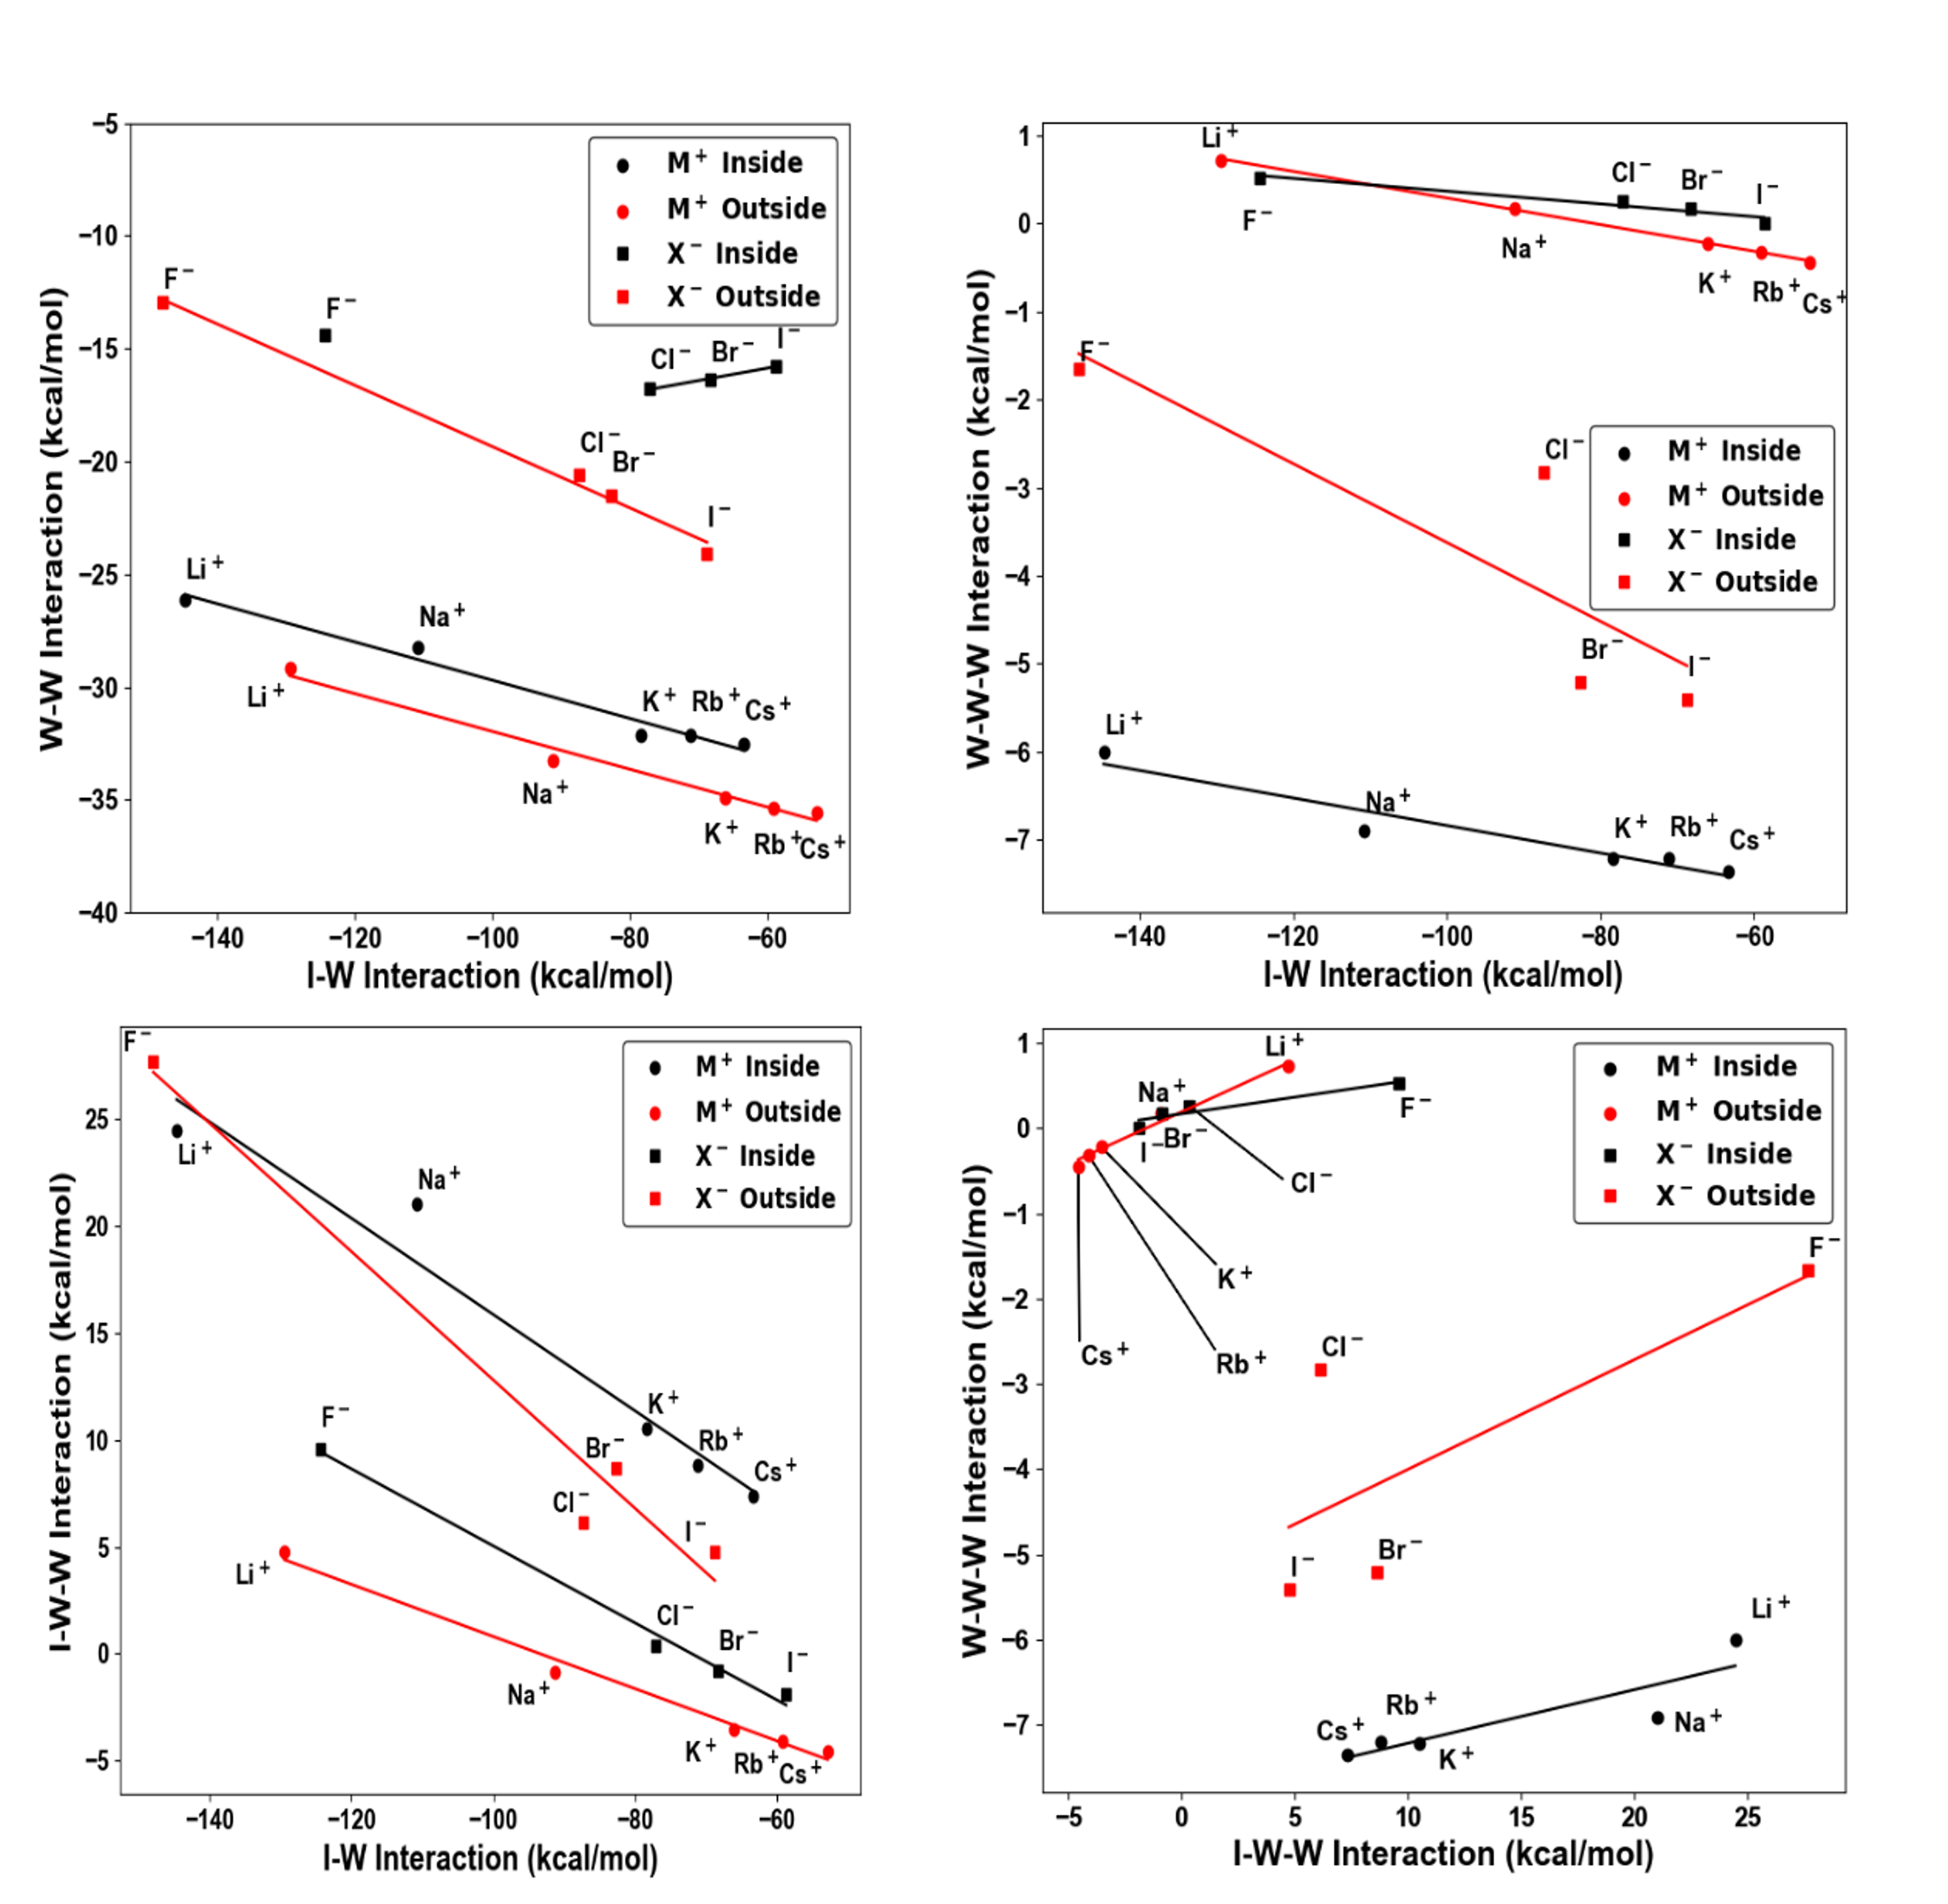
\includegraphics[width=.9\textwidth]{Figures/Chapter_3/figure_9_combined.png}
  \caption[Correlations between the various interactions for the \ce{Z^{+/-}(H2O)9}, \ce{Z} = \ce{M^+} (\ce{Li^+}, \ce{K^+}, \ce{Cs^+}) and \ce{Z} = \ce{X^-} (\ce{Cl^-}, \ce{Br^-}, \ce{I^-}) clusters. (a) Top left panel: (W-W) vs. (I-W), (b) top right panel: (W-W-W) vs. (I-W), (c) bottom left panel: (I-W-W) vs. (I-W) and (d) bottom right panel: (I-W-W) vs. (W-W-W) interactions.]{Correlations between the various interactions for the \ce{Z^{+/-}(H2O)9}, \ce{Z} = \ce{M^+} (\ce{Li^+}, \ce{K^+}, \ce{Cs^+}) and \ce{Z} = \ce{X^-} (\ce{Cl^-}, \ce{Br^-}, \ce{I^-}) clusters. (a) Top left panel: (W-W) vs. (I-W), (b) top right panel: (W-W-W) vs. (I-W), (c) bottom left panel: (I-W-W) vs. (I-W) and (d) bottom right panel: (I-W-W) vs. (W-W-W) interactions.}
  \label{fig:MBE_II_9}
\end{figure}

\begin{table}[t]
\begin{adjustbox}{width=\columnwidth,center}
\begin{tabular}{@{}ccccccccc@{}}
\toprule
\multicolumn{2}{l}{\textbf{Cluster}} & \textbf{Binding Energy} & \textbf{Total 2-B} & \textbf{I-W}     & \textbf{W-W}    & \textbf{Total 3-B} & \textbf{I-W-W} & \textbf{W-W-W}  \\ \hline
                  & \multicolumn{8}{c}{\textbf{\ce{Li^+(H2O)9}}}                                                                                                                                                                                        \\ \hline
\multicolumn{2}{l}{Ion inside}       & -154.44        & -170.78                                                                & -144.68 & -26.10 & 18.46                                                               & 24.46 & -6.00  \\
\multicolumn{2}{l}{Ion outside}      & -151.62        & -158.65                                                                & -129.46 & -29.20 & 5.46                                                                & 4.736 & 0.72   \\ \hline
                  & \multicolumn{8}{c}{\textbf{\ce{K^+(H2O)9}}}                                                                                                                                                                                         \\ \hline
\multicolumn{2}{l}{Ion inside}       & -107.52        & -110.48                                                                & -78.357 & -32.12 & 3.29                                                                & 10.51 & -7.22  \\
\multicolumn{2}{l}{Ion outside}      & -102.88        & -101.03                                                                & -66.10  & -34.93 & -3.76                                                               & -3.54 & -0.22  \\ \hline
                  & \multicolumn{8}{c}{\textbf{\ce{Cs^+(H2O)9}}}                                                                                                                                                                                        \\ \hline
\multicolumn{2}{l}{Ion inside}       & -95.42         & -95.92                                                                 & -63.38  & -32.54 & -0.01                                                               & 7.35  & -7.36  \\
\multicolumn{2}{l}{Ion outside}      & -91.45         & -88.40                                                                 & -52.85  & -35.55 & -4.99                                                               & -4.54 & -0.45  \\ \hline
                  & \multicolumn{8}{c}{\textbf{\ce{Cl^-(H2O)9}}}                                                                                                                                                                                        \\ \hline
\multicolumn{2}{l}{Ion inside}       & -91.06         & -93.92                                                                 & -77.14  & -16.78 & 0.62                                                                & 0.365 & 0.26   \\
\multicolumn{2}{l}{Ion outside}      & -102.77        & -107.94                                                                & -87.33  & -20.61 & 3.31                                                                & 6.13  & -2.82  \\ \hline
                  & \multicolumn{8}{c}{\textbf{\ce{Br^-(H2O)9}}}                                                                                                                                                                                        \\ \hline
\multicolumn{2}{l}{Ion inside}       & -83.26         & -84.66                                                                 & -68.27  & -16.39 & -0.657                                                              & -0.83 & 0.17   \\
\multicolumn{2}{l}{Ion outside}      & -99.23         & -104.21                                                                & -82.69  & -21.52 & 3.45                                                                & 8.65  & -5.20  \\ \hline
                  & \multicolumn{8}{c}{\textbf{\ce{I^-(H2O)9}}}                                                                                                                                                                                         \\ \hline
\multicolumn{2}{l}{Ion inside}       & -74.70         & -74.46                                                                 & -58.70  & -15.76 & -1.86                                                               & -1.87 & 0.004  \\
\multicolumn{2}{l}{Ion outside}      & -91.70         & -92.83                                                                 & -68.76  & -24.08 & -0.66                                                               & 4.75  & -5.41  \\ \hline
                  & \multicolumn{8}{c}{\textbf{\ce{(H2O)_{10}}}}                                                                                                                                                                                          \\ \hline
\multicolumn{2}{l}{}                 & -82.42         & -62.76                                                                 & n/a     & -62.76 & -21.69                                                              & n/a   & -21.69 \\ \bottomrule
\end{tabular}
\end{adjustbox}
\begin{spacing}{1.0}
\caption[MBE analysis (kcal/mol) for the \ce{Z^{+/-}(H2O)9} clusters, \ce{Z} = \ce{Li^+}, \ce{K^+}, \ce{Cs^+}, \ce{Cl^-}, \ce{Br^-}, \ce{I^-}, at the MP2/aVDZ level including corrections for BSSE.]{MBE analysis (kcal/mol) for the \ce{Z^{+/-}(H2O)9} clusters, \ce{Z} = \ce{Li^+}, \ce{K^+}, \ce{Cs^+}, \ce{Cl^-}, \ce{Br^-}, \ce{I^-}, at the MP2/aVDZ level including corrections for BSSE.}\label{tab:MBE_II_T2}
\end{spacing}
\end{table}

\par The top right panel, \ref{fig:MBE_II_9}(b), traces the anti-correlation between the total 2-B (I-W) and the total 3-B (W-W-W) term: stronger ion-water interactions result in a weaker water 3-B term. Similarly, a linear anti-correlation exists between the 2-B (I-W) and the 3-B (I-W-W) interactions shown in the bottom right panel, \ref{fig:MBE_II_9}(c): stronger (I-W) interactions induce more repulsive (destabilizing) (I-W-W) interactions with the \ce{X^-} ion outside structures the only ones deviating from linearity. Finally, there also seems to be a linear (save the \ce{X^-} outside cluster isomers) anti-correlation between the two components of the 3-B term, viz. (I-W-W) and (W-W-W), which is shown in panel 9(d). The correlations shown in panels \ref{fig:MBE_II_9}(b)-(d) suggest a universal behavior of the ions considered in this study with the exception of the 3-B (I-W-W) and (W-W-W) for the ion outside isomer of \ce{Cl^-}. If the magnitudes of these total 3-B terms for that isomer of \ce{Cl^-} were in line with the ones for the other two halide ions there would be a remarkable correlation between all terms with the same slope! We ensured that the 3-B results for that cluster are accurate and we will plan to investigate this behavior in future studies by including other monatomic anions in the set. The above findings further validate the discussion in Section \ref{sec:MBE_2_sec_3a} regarding anti-cooperative effects between the ion-water and water-water interactions and provide a quantitative account of this effect.

\subsection{Modeling of the BSSE Corrections:}
\par In order to explore the effects of BSSE on the MBE for aqueous ionic clusters, we have calculated the 2-B contribution to the BSSE correction for the \ce{Z^{+/-}(H2O)9} clusters, where \ce{Z} = \ce{Li^+}, \ce{K^+}, \ce{Cs^+}, \ce{Cl^-}, \ce{Br^-}, \ce{I^-} at the MP2/aVDZ level. We have split the BSSE-correction into contributions from water-water and ion-water dimers, and then fit the resulting curves using the same error function formula presented in our previous work, viz. $BSSE(R_{ij})=A[1+erf(-BR_{ij})]$, where $R_{ij}$ is the pair distance between the oxygen atoms of fragments $i$ and $j$ and $A$ and $B$ are fitting parameters.

\begin{figure}[t]
\uwsinglespace
\centering
\begin{adjustbox}{max size={.6\textwidth}{.6\textheight}}
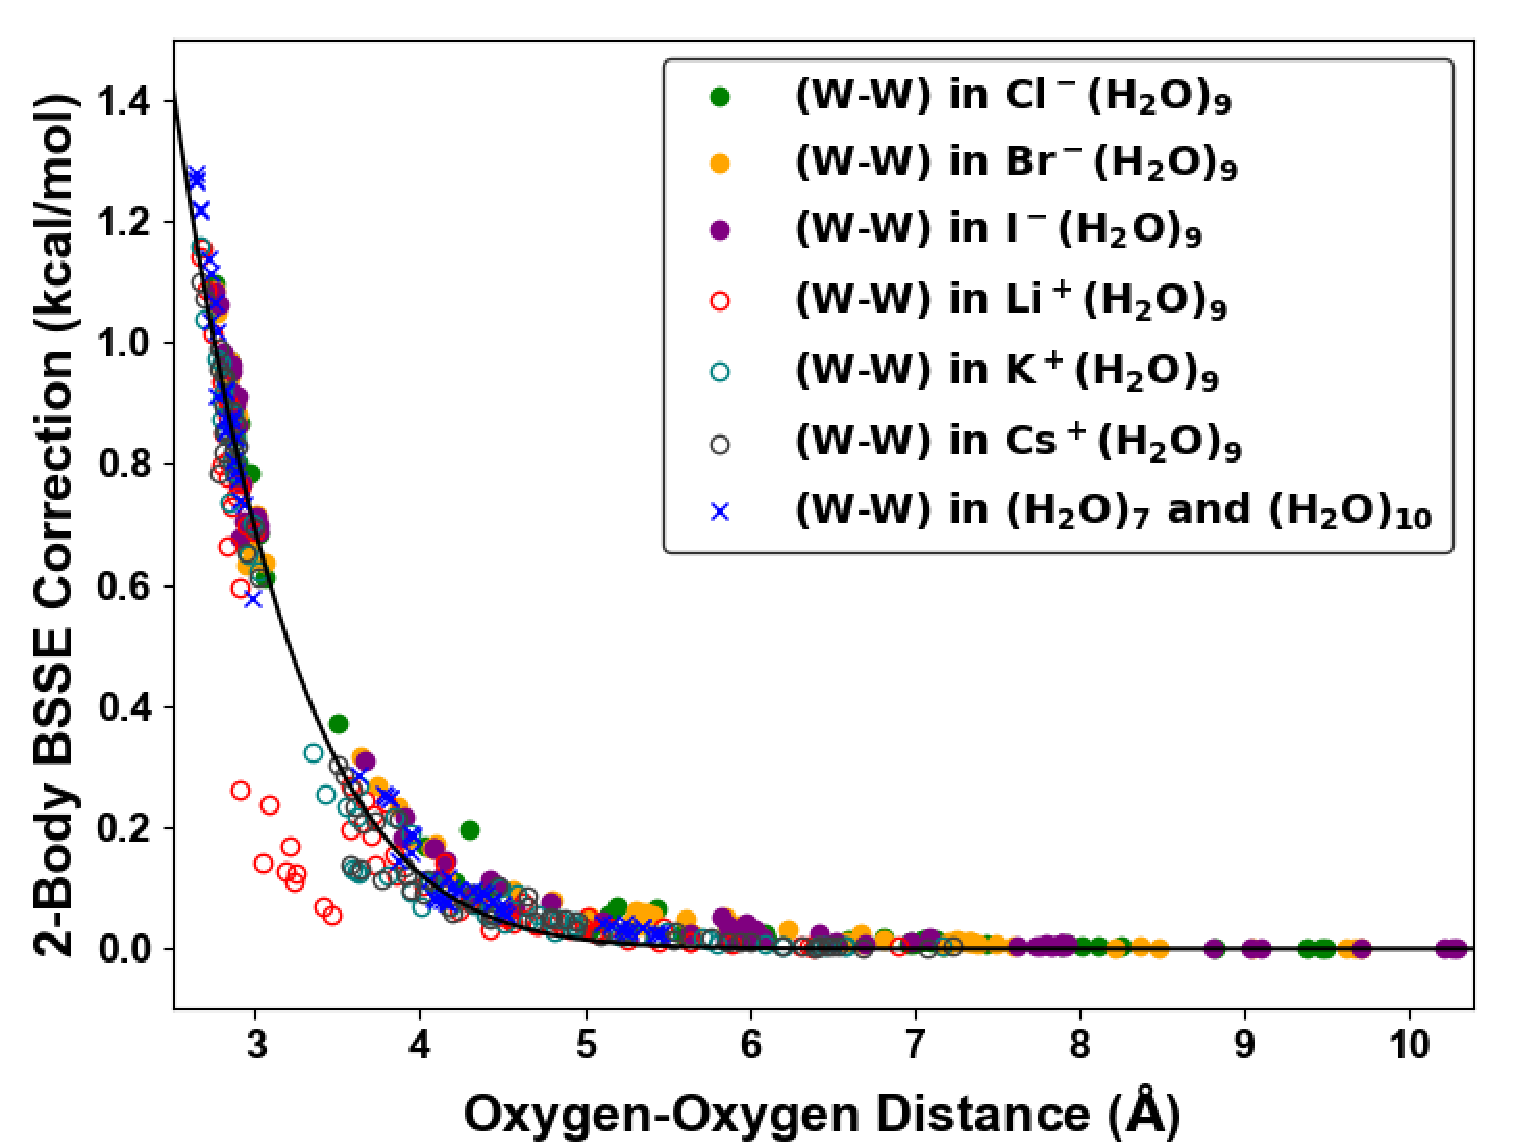
\includegraphics[width=\textwidth]{Figures/Chapter_3/figure_10.pdf}
\end{adjustbox}
\begin{spacing}{1.0}
\caption[2-Body BSSE correction for all 498 water dimers extracted from the \ce{Z^{+/-}(H2O)9}, \ce{Z} = \ce{Li^+}, \ce{K^+}, \ce{Cs^+}, \ce{Cl^-}, \ce{Br^-}, \ce{I^-}, clusters as well as the two neutral water clusters \ce{(H2O)7} and \ce{(H2O)_{10}} as a function of the Oxygen – Oxygen distance.]{2-Body BSSE correction for all 498 water dimers extracted from the \ce{Z^{+/-}(H2O)9}, \ce{Z} = \ce{Li^+}, \ce{K^+}, \ce{Cs^+}, \ce{Cl^-}, \ce{Br^-}, \ce{I^-}, clusters as well as the two neutral water clusters \ce{(H2O)7} and \ce{(H2O)_{10}} as a function of the Oxygen – Oxygen distance. The solid line represents a fit to the function $BSSE(R_{ij})=A[1+erf(-BR_{ij})]$ yielding the parameters $A = 13.346$ and $B = 0.457$. The water dimers extracted from the two isomers of the \ce{Li^+(H2O)9} clusters were not included in the fit. See text for details.}\label{fig:MBE_II_10}
\end{spacing}
\end{figure}

\par Figure \ref{fig:MBE_II_10} shows the variation of the 2-B BSSE contribution from all water-water only nearest neighbor and distant pairs, extracted from the various ion-water clusters, as well as from the \ce{(H2O)7} and \ce{(H2O)_{10}} clusters reported in the previous paper of this series,\autocite{heindel_many-body_2020} as a function of the Oxygen – Oxygen distance in each pair. Note that this is for the 498 water dimer pairs, which have been evaluated in the full cluster basis to account for the 2-B contribution to the total BSSE, without considering any ion-water pairs. The solid line corresponds to a least-mean-squares fit of the data (save the water dimers extracted from the \ce{Li^+(H2O)9} clusters) to the error function above, yielding the parameters $A = 13.346$ and $B = 0.457$ ($R^2 = 0.985$). Note that the water dimers in both the pure water and ion-water pairs follow the same trend, a fact that suggests the validity of this approximation for the BSSE due to the water-water interaction in heterogeneous systems. There are clearly some outlier points near the shoulder of the curve in Figure \ref{fig:MBE_II_10} corresponding to water dimer pairs extracted from the \ce{Li^+(H2O)9} clusters. These points turn out to be all water dimer pairs where both water molecules are nearest neighbors of the \ce{Li^+} cation. Because cations are solvated via the oxygen atom and \ce{Li^+} is very compact, these are quite unusual dimers, in which two oxygen atoms point at each other and are close to one another. This type of peculiar intermolecular arrangement is only likely to be sampled for the \ce{Li^+(H2O)9} clusters, so we have omitted them from the fit to the rest of the data. Nonetheless, the above discussion provides a justification of the reason these outliers occur.

\begin{figure}[t]
\uwsinglespace
\centering
\begin{adjustbox}{max size={.6\textwidth}{.6\textheight}}
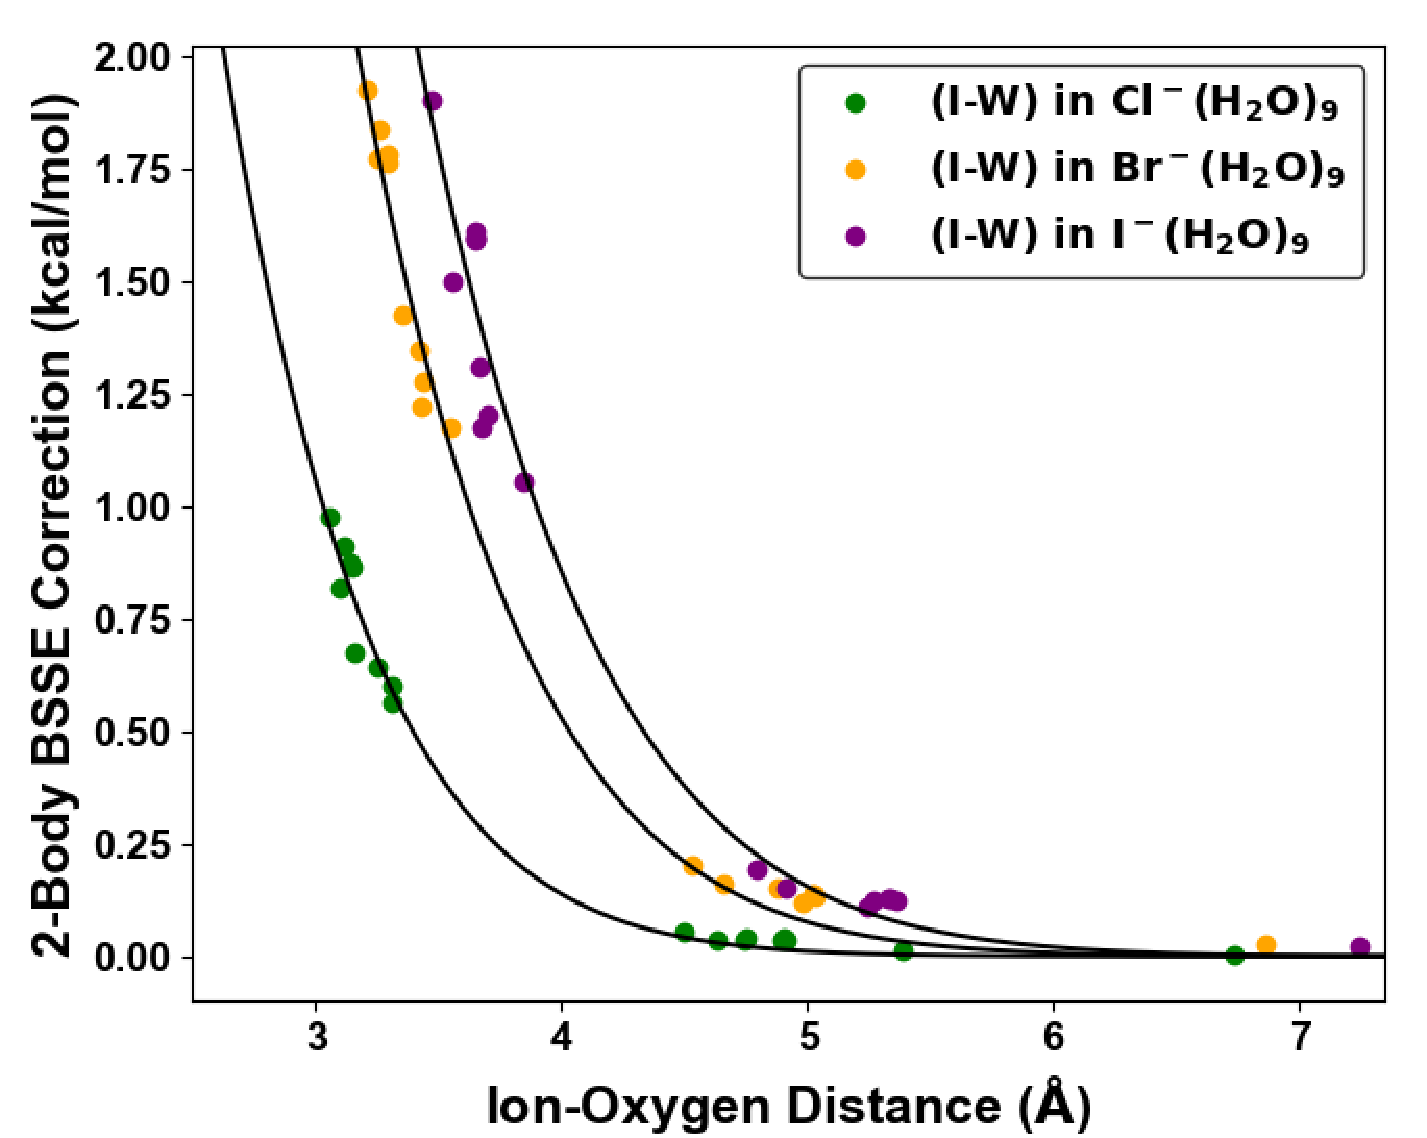
\includegraphics[width=\textwidth]{Figures/Chapter_3/figure_11.pdf}
\end{adjustbox}
\begin{spacing}{1.0}
\caption[2-B BSSE correction for all 54 ion - water dimers extracted from the \ce{Z-(H2O)9}, where \ce{Z} = \ce{Cl^-}, \ce{Br^-}, \ce{I^-}, clusters.]{2-B BSSE correction for all 54 ion - water dimers extracted from the \ce{Z-(H2O)9}, where \ce{Z} = \ce{Cl^-}, \ce{Br^-}, \ce{I^-}, clusters. The solid lines represents fits to the function $BSSE(R_{ij})=A[1+erf(-BR_{ij})]$ yielding the parameters  $A_{\ce{F^-}} = 12.161$, $B_{\ce{F^-}} = 0.469$; $A_{\ce{Cl^-}} = 33.831$, $B_{\ce{Cl^-}} =0.507$; $A_{\ce{Br^-}} = 42.159$, $B_{\ce{Br^-}} = 0.441$; $A_{\ce{I^-}} = 43.118$, $B_{\ce{I^-}} = 0.412$.}\label{fig:MBE_II_11}
\end{spacing}
\end{figure}

\par The corresponding 2-B BSSE contributions originating from the 54 ion-water pairs extracted from the \ce{Z^-(H2O)9}, \ce{Z} = \ce{Cl^-}, \ce{Br^-}, \ce{I^-}, ionic clusters are shown in Figure \ref{fig:MBE_II_11} as a function of the Ion – Oxygen distance. In contrast to the case of neutral water dimers, where each point falls on essentially the same curve (cf. Figure \ref{fig:MBE_II_10}) regardless of the system (pure water or aqueous ionic cluster) the water dimer is extracted from, in the case of anion-water dimers each different system’s dimers fall on separate curves, thus having different BSSE profiles. Each of these curves can still be fit with the same functional form ($erf$) previously used for the water dimers yielding the parameters $A_{\ce{F^-}}=12.161$, $B_{F^-}=0.469$ ($R^2=0.983$); $A_{\ce{Cl^-}}=33.831$, $B_{Cl^-}=0.507$ ($R^2 = 0.987$); $A_{\ce{Br^-}}=42.159$, $B_{\ce{Br^-}}=0.441$ ($R^2 = 0.992$); $A_{\ce{I^-}}=43.118$, $B_{\ce{I^-}}=0.412$ ($R^2 = 0.975$) for the three different cases. This result produces different BSSE profiles between the different ions and also between the ion-water and water-water interactions.

\begin{figure}[h]
\uwsinglespace
\centering
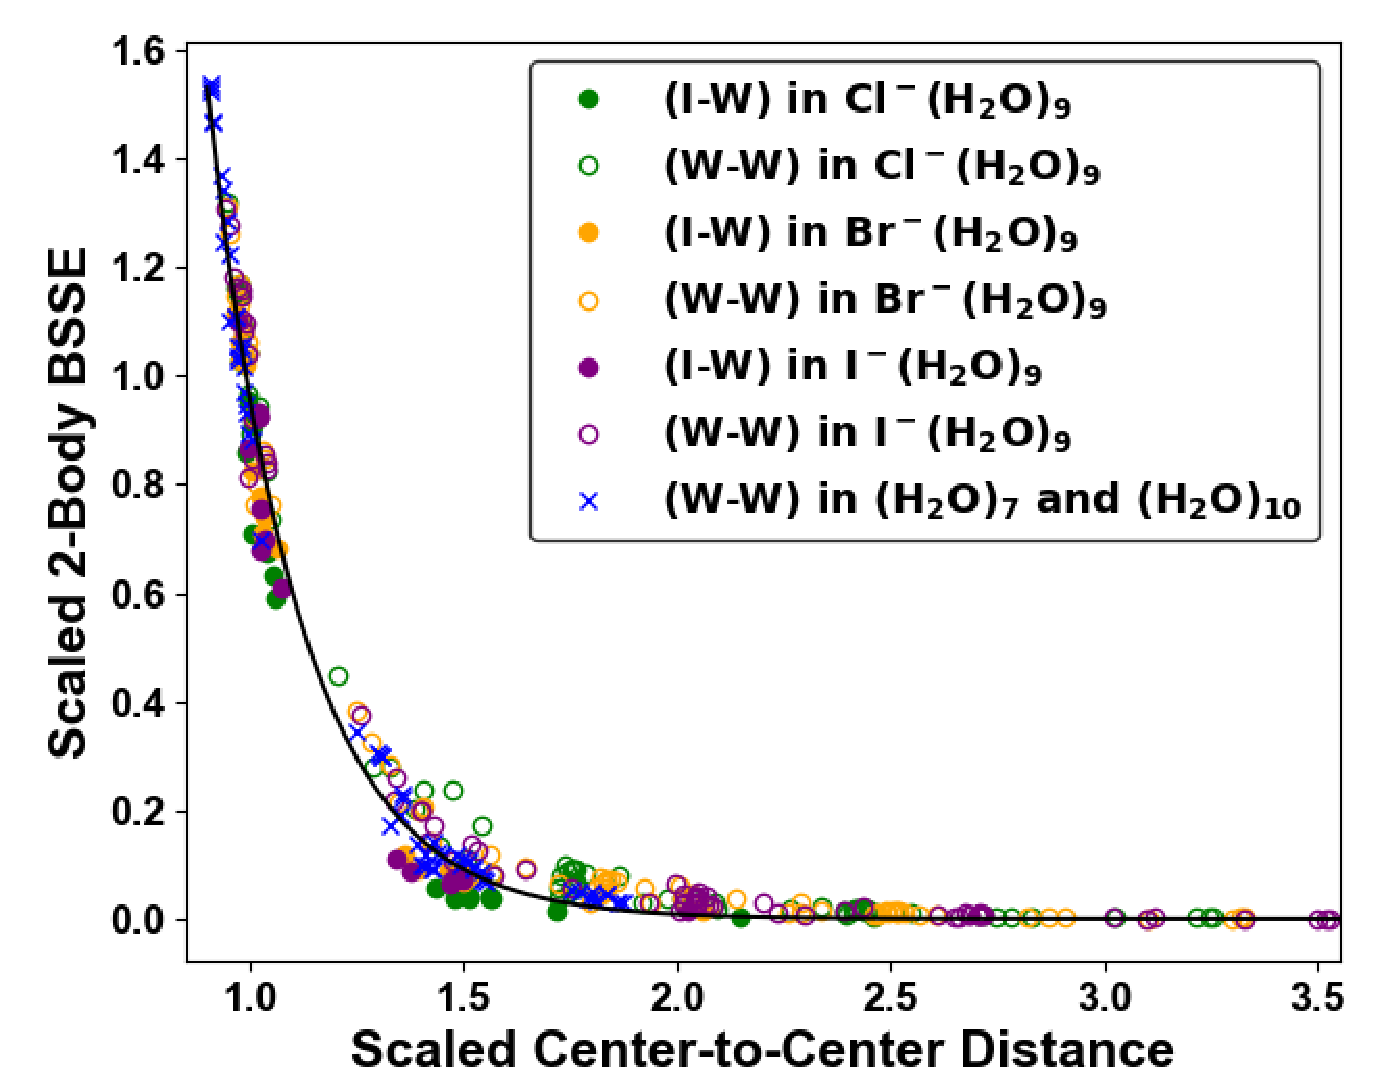
\includegraphics[width=.8\textwidth]{Figures/Chapter_3/figure_12.pdf}
\caption[Scaled 2-Body BSSE values for all 336 ion-water and water-water dimers cut from \ce{Z^-(H2O)9} where \ce{Z} = \ce{Cl^-}, \ce{Br^-}, and \ce{I^-} as well as two neutral water clusters of \ce{(H2O)7} and \ce{(H2O)_{10}}. Each energy is scaled by the size of the BSSE-correction of the corresponding \ce{Z^-(H2O)} dimer or that of a neutral water dimer. Each distance is scaled by the equilibrium center-to-center distance in those same dimers. See text for more detail.]{Scaled 2-Body BSSE values for all 336 ion-water and water-water dimers cut from \ce{Z^-(H2O)9} where \ce{Z} = \ce{Cl^-}, \ce{Br^-}, and \ce{I^-} as well as two neutral water clusters of \ce{(H2O)7} and \ce{(H2O)_{10}}. Each energy is scaled by the size of the BSSE-correction of the corresponding \ce{Z^-(H2O)} dimer or that of a neutral water dimer. Each distance is scaled by the equilibrium center-to-center distance in those same dimers. See text for more detail.}
\label{fig:MBE_II_12}
\end{figure}

\par In order to consolidate the previous results seeking a universal BSSE profile as a function of the distance between dissimilar pairs irrespective of the system, we rely on the use of reduced distances and energy scales. This approach, when applied to commonly used interaction potential functions describing intermolecular interactions such as Mie, Lennard-Jones, Morse, Buckingham exponential-6 or the Buffer-2 potential, has been shown to produce universal potential energy functions for alkali metal-water and halide-water interactions.\autocite{werhahn_universal_2014,werhahn_new_2015,xantheas_universal_2014}  In these previous studies, the reduced coordinates were chosen as $r^*=(r/r_e)$ and $V^*(r)=V(r)/V(r_e)$ , where $r_e$ is the intermolecular equilibrium distance between the two fragments and $V(r_e)$ is the corresponding potential energy at the dimer minimum geometry. We have performed a similar scaling of the 2-body BSSE correction, where the center-to-center distance is scaled by the equilibrium distance of the corresponding dimers. For example, each X-O distance is scaled by the MP2/aVDZ equilibrium distance of the \ce{X^-(H2O)} dimer. Similarly, the 2-body BSSE values are scaled by the magnitude of the BSSE correction, $D_e^{BSSE}-D_e$, when calculating the BSSE-corrected binding energy at the dimer minimum geometry. We have done this for all of the water-water and halide-water dimers extracted from all of the clusters considered in this study. The BSSE profile for these 388 points is shown in Figure \ref{fig:MBE_II_12}. This scaling makes the 2-body BSSE-correction profile universal for the systems we have considered. Clearly, different parameters are needed for each level of theory and basis set, but this only requires additional calculations on just dimers. This universal curve can be fit with either an exponential or an error function. For consistency, we show the fit to an error function in Figure \ref{fig:MBE_II_12} with parameters $A = 16.709$, $B = 1.341$ ($R^2 = 0.984$), but the exponential fit may be slightly better in this case with parameters $A = 104.774$, $B = 4.696$ ($R^2 = 0.987$).

\section{Conclusions} \label{sec:MBE_2_sec_4}

\par The effect of ions on the structure of water remains a very important open topic, which is relevant to understanding various biological processes, reactions in charged nanodroplets, the development of \textit{ab initio} force fields, and several other scientific areas. In an effort to further understand the interplay between ion-water and water-water interactions, we have investigated the MBE in aqueous ionic clusters and compared the results for these systems with the ones we have previously reported for pure water clusters. Specifically, we have studied structural arrangements in which representative alkali metal cations (\ce{Li^+}, \ce{K^+}, \ce{Cs^+}) or halide anions (\ce{Cl^-}, \ce{Br^-}, \ce{I^-}) reside on either the inside or the outside of a water cluster. The calculations were performed at the MP2 level of theory with basis sets that systematically converge to the CBS limit in order to investigate the behavior of the magnitude of the MBE terms with the size of the basis set. One specific focus of the present study was to understand the correlation between the ion-water and water-water interactions and gain insight into the manner that ion-water interactions affect the strength of the neighboring hydrogen bonded water network.

\par The major takeaways from an analysis of the water-water and ion-water terms of the MBE are summarized as follows: (i) the 2-B term dominates in ion-water systems, compared to neutral water systems of similar size, (ii) the 3-B term is usually smaller as a percentage of the cluster binding energy and in addition it is of opposite sign than for neutral water systems, independent of ion position or identity in the clusters we examined, (iii) the 4-B and higher terms are essentially negligible. The exception is the case when \ce{Li^+} resides on the inside of the water cluster. We note that this cluster has by far the largest 2-B (I-W) term both in terms of magnitude and percentage, but this also results in a diminished 2-B (W-W) interactions. This anomaly carries through the 3-B term which is large and repulsive for (I-W-W) interactions (-15.6\% of $D_e$) with a slightly stabilizing 4-B (I-W-W-W) term (3.0\% of $D_e$). We ascribe these results to the ability of cations to destroy the cooperativity of hydrogen-bonding in a water network by making water molecules donate through the oxygen atoms, (iv) there exist remarkable anti-correlations between the total 2-B (I-W) and (W-W) interactions, demonstrating the effect of strong ion-water interactions in disrupting the water network and weaken the water-water interactions. This anti-correlation effect is also carried into the effect of the (I-W) to the 3-B (W-W-W) interaction. A universal behavior for all ions considered in this study seems to emerge from the analysis of these correlations, (v) the variation of the MBE terms higher than k = 4 with basis set is quite similar to the one previously reported for pure water clusters: they exhibit an undulating behavior around zero gradually diminishing in magnitude with increasing basis set towards the CBS limit and this behavior is corrected upon inclusion of BBSE corrections, (vi) electron correlation was found to mainly affect the 2-B term and by neglecting the correlation contribution in all terms above the 3-body results in a small error $O$(\textless 0.6\%).

\par Furthermore, we have verified and expanded the previously proposed means of approximating the 2-B portion of the BSSE correction via an error function, which is only a function of the intermolecular distance between the centers of anion-water systems and water-water dimers. In the case of water dimers cut from clusters containing an ion, we verified that the BSSE follows the same trend as in the case of neutral water clusters. The BSSE correction for anion-water dimers each fall on their own profile but are fit well by the same functional form as for water dimers. We have shown that a simple scaling of the center-to-center distance and BSSE correction by reference values taken from gas-phase optimized dimers results in a universal BSSE profile with respect to the intermolecular center-to-center distance that describes both the water-water and halide-water nearest neighbor and distant dimers. We do realize that some of the conclusions are constrained by the limited sampling of configurations used in this study. In the future, we aspire to enhance the configurational sampling for the MBE analysis by considering clusters that are extracted from aqueous phase molecular dynamics trajectories.

\chapter{The many-body expansion for aqueous systems: III. Water cages of clathrate hydrates}
\label{ch:clathrates}

\section{Introduction}

\par Entropy changes are an important component in understanding the thermodynamics of chemical phenomena and processes, which are thermodynamically driven by negative free energies. A negative free energy is equivalent to stating that entropy is produced throughout the process. The absolute entropy of a system depends on the total number of microstates, $\Omega$, accessible to the system, viz. $S=k_B\ln\Omega$. This means that entropy nearly always increases with temperature as more phase space is accessible at higher temperatures. It is therefore tempting to assume the converse and say that as temperature goes to zero, entropy must also go to zero. However, even at zero temperature, it is possible for multiple microstates to be accessible, resulting in the so-called residual entropy popularized by Linus Pauling in his analysis of molecular crystals.\autocite{pauling_structure_1935}

\par In hydrogen bonded systems like ice, which have directional hydrogen bonds that may be microscopically distinct but result in macroscopically identical crystals (such as for instance for the proton disordered ice phases), the residual entropy arises from the number of those microscopically distinct microstates corresponding to the different hydrogen bonded configurations, which, in the case of ice, satisfy the Bernal-Fowler ice rules.\autocite{bernal_theory_1933} The topic of residual entropy is of particular interest as it explicitly connects molecular microstates (distinct hydrogen bonding networks) to macroscopic (crystal) structures. In the following we will use the term microstate to denote a particular arrangement of the hydrogen atoms in an oxygen atom framework according to the ice rules.

\par In this study, we present a comprehensive study of the molecular microstates making up the water cages that are the building blocks of the clathrate hydrate lattices, with a particular focus on their multiplicities and their energetics. Clathrate hydrates are well-studied, quite fascinating heterogeneous crystals, in which water solidifies around a guest molecule such as hydrogen, methane or carbon dioxide\autocite{sloan_jr_clathrate_2007,arjmandi_equilibrium_2007,english_structural_2003}. Naturally occurring gases crystallize in three clathrate hydrate crystal lattices known as sI (cubic, Pm3 $\overline{n}$), sII (cubic, Fd3 $\overline{m}$), and sH (hexagonal, P6/mmm). These are made up with combinations of fused cages of\autocite{sloan_jr_clathrate_2007}
	
	\par (i) the \textit{pentagonal dodecahedron} or D-cage \ce{(H2O)_{20}}: 20 water molecules forming a hollow cage with 12 pentagonal faces ($5^{12}$), 
	
	\par (ii) the \textit{irregular dodecahedron} \ce{(H2O)_{20}}: 20 water molecules forming a hollow cage with 3 tetragonal, 6 pentagonal, and 3 hexagonal faces ($4^35^66^3$),
	
	\par (iii) the \textit{tetrakaidecahedron} or T-cage \ce{(H2O)_{24}}: 24 water molecules forming a hollow cage with 12 pentagonal and 2 hexagonal faces ($5^{12}6^2$),
	
	\par (iv) the \textit{hexakaidecahedron} or H-cage \ce{(H2O)_{28}}: 28 water molecules forming a hollow cage with 12 pentagonal and 4 hexagonal faces ($5^{12}6^4$) and
	
	\par (v) the \textit{icosahedron} \ce{(H2O)_{36}}: 36 water molecules forming a hollow cage with 12 pentagonal and 8 hexagonal faces ($5^{12}6^8$).

\par The unit cell of the sI hydrate lattice is made up with 2 units of $5^{12}$ and 6 units of $5^{12}6^2$ cages, whereas the one of the sII hydrate is made up with 16 units of $5^{12}$ and 8 units of $5^{12}6^4$ cages. Finally, the unit cell of the sH hydrate is made up of 3 units of $5^{12}$, 2 units of $4^35^66^3$ and 1 unit of $5^{12}6^8$ cages.\autocite{sloan_jr_clathrate_2007} In this study we will restrict our discussion to the D-cage $5^{12}$, T-cage $5^{12}6^2$ and H-cage $5^{12}6^4$, which are the building blocks of the sI and sII naturally occurring hydrate lattices.\autocite{sloan_jr_clathrate_2007} The macroscopic structure of each of these lattices is only determined up to placement of the oxygen atoms in the crystal structure just as in the case of the ice phases with proton disorder. This means that clathrate hydrates will have a residual entropy related to the number of hydrogen bonding arrangements in each cage, as well as the number of ways to stitch these cages together\autocite{yoo_low-energy_2009} in a way that is consistent with the observed crystal structure. For the residual entropy of the \ce{(H2O)_{20}} cage an estimate of $S_0=Nk_B\cdot\ln(\frac{3}{\sqrt{2}})=0.75204\cdot Nk_B$, where $N$ is the number of molecules and $k_B$ is Boltzmann's constant, has been previously reported.\autocite{kirov_identifying_2008,kirov_f-structure_1994} This is about 85\% more than the residual entropy of hexagonal ice.\autocite{pauling_structure_1935} Notice that each of the \ce{(H2O)_{20}}, \ce{(H2O)_{24}}, and \ce{(H2O)_{28}} cages have the same residual entropy when estimated using Pauling’s approach.\autocite{pauling_structure_1935} We will discuss this in more detail later along with the connection between residual entropy and the energetics of each microstate.

\par In the following, we will briefly summarize symmetry considerations and topological descriptors that aid in reducing the vast number of available microstates and assist in the identification of the unique, symmetry-distinct, low-lying energy microstates that are present in the D-, T- and H-cages.

\subsection{Symmetry considerations}

\begin{figure}[t]
\uwsinglespace
\begin{center}
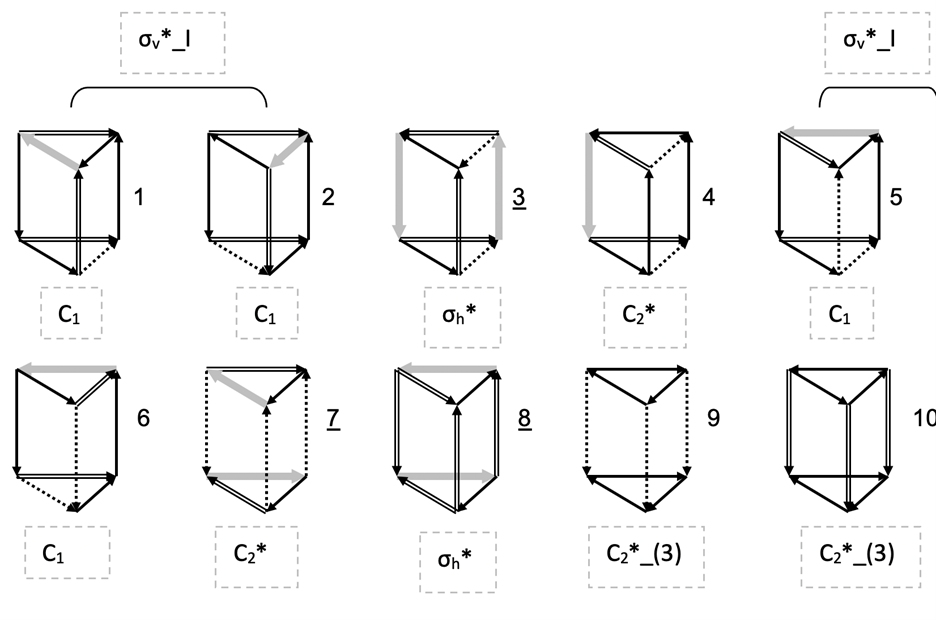
\includegraphics[width=\textwidth]{Figures/Chapter_6/symmetry_configurations.png}
\end{center}
\begin{spacing}{1.0}
\caption[Symmetry isomers of all possible microstates of the water hexamer prism.]{Symmetry isomers of all possible microstates of the water hexamer prism.}\label{fig:MBE_III_F1}
\end{spacing}
\end{figure}

\par For every microstate of a polyhedral water cluster, there exists another one in which all hydrogen bonds have exactly the opposite direction. This duality allows dividing the set of all microstates into pairs of antipodes. It is oftentimes the case that antipodal microstates are connected by a symmetry operation such as rotation around a symmetry axis or reflection with respect to a symmetry plain. An illustration of this property for the hexamer prism water cluster is shown in Figure \ref{fig:MBE_III_F1}, where antipodal microstates are either connected via a symmetry operation or not are shown. Antipodes connected via a symmetry operation are physically equivalent since they represent the same molecular structure. Most often, however, changing the direction of all H-bonds leads to a new microstate that is not related to the initial one by any symmetry operation. In this case, the antipodes represent different, physically non-equivalent microstates. 

\par Reversing the direction of all H-bonds can be considered as an additional operation of generalized symmetry, more precisely that of antisymmetry. The hydrogen-bond-reversal symmetry\autocite{kirov_hydrogen-bond-reversal_2016} is one example of the general concept of antisymmetry, along with the black-and-white symmetry\autocite{shubnikov_symmetry_1951,mackay_extensions_1957} and the magnetic symmetry.\autocite{hamermesh_group_2012,lifshitz_statistical_2013} To describe the hydrogen-bond-reversal symmetry, it is convenient to rely on the widely used magnetic symmetry groups.\autocite{litvin_magnetic_2013} The two types of microstates discussed above can be classified as antisymmetric and ordinary ones, respectively. The antisymmetric microstates have elements of extended symmetry (antisymmetry), which, along with rotation or reflection operations, also include the hydrogen-bond reversal (antiidentity).
	
\par In the set of all the non-isomorphic (non-equivalent by symmetry) microstates, for each ordinary configuration there is a direct antipode that differs only by the direction of all hydrogen bonds (antiidentity). In the set of all 3,600,000 isomorphic microstates of the D-cage,\autocite{kirov_atlas_2002} each has a direct antipode (opposite direction of all hydrogen bonds). However, in the set of 30,026 non-isomorphic symmetry distinct microstates, each one represents a whole class of isomorphic structures differing from each other by reflection or rotation. These representatives can be chosen arbitrarily. In this set, the antipodes sometimes differ only in the direction of hydrogen bonds; however, for a complete superposition of antipodal structures, one will most likely need to additionally rotate the configuration or reflect it in a certain plane. These configurations are related to each other by the antisymmetry operation, which consist of first reversing all hydrogen bonds and then applying some operation of ordinary symmetry. In this manner, the antipodal configurations are referred to as the antisymmetry pairs. Thus, there are two types of proton configurations: antisymmetrical and nonantisymmetrical (ordinary). The antipode configurations are very similar in their properties, while at the same time are not being identical.

\subsection{The Strong-Weak Effective Bond (SWEB) model}

\begin{figure}[t]
\uwsinglespace
\begin{center}
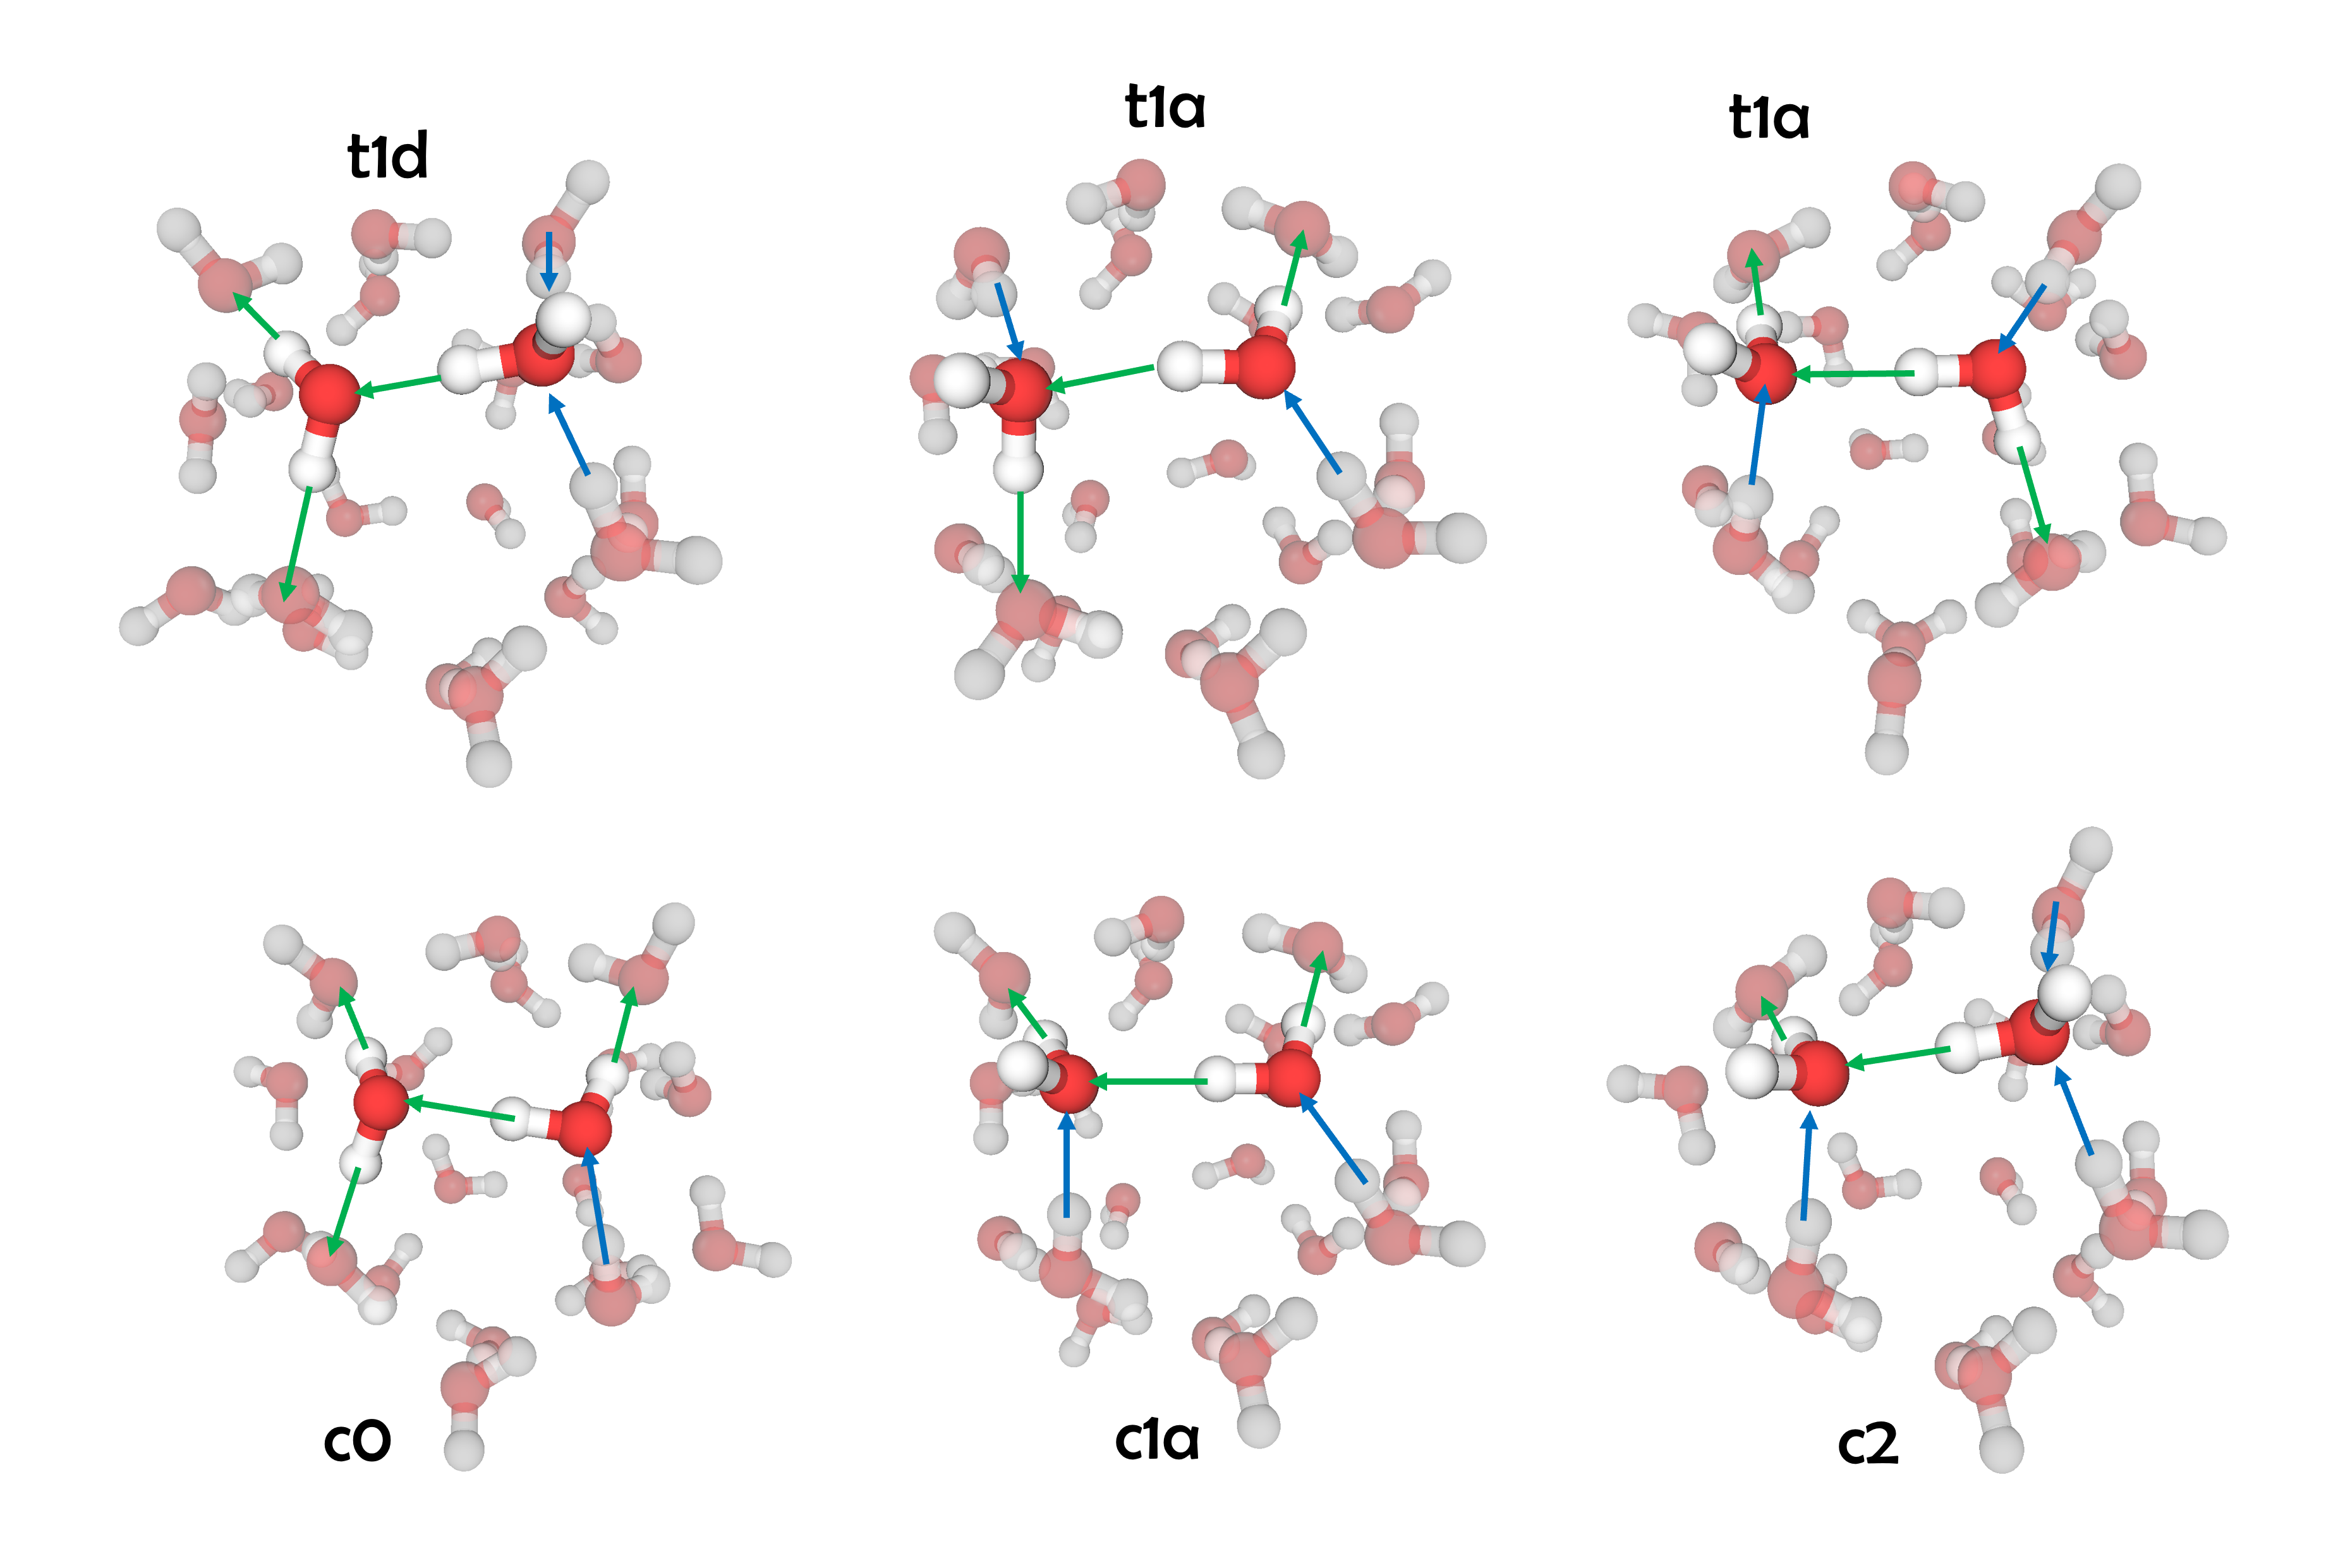
\includegraphics[width=\textwidth]{Figures/Chapter_6/sweb_types.png}
\end{center}
\begin{spacing}{1.0}
\caption[Classification of hydrogen bonds depending on the dimer orientation on the polyhedral surface. Symbols denote trans (t) or cis (c) arrangements and number of hydrogen bonds on either the donor (d) or the acceptor (a) molecules. In the above notation t1d denotes a trans orientation with 1 free OH bond on the hydrogen bond donor molecule. The D-, T- and H-cages have a maximum of 7, 9 and 11 t1d dimers.]{Classification of hydrogen bonds depending on the dimer orientation on the polyhedral surface. Symbols denote trans (t) or cis (c) arrangements and number of hydrogen bonds on either the donor (d) or the acceptor (a) molecules. In the above notation t1d denotes a trans orientation with 1 free OH bond on the hydrogen bond donor molecule. The D-, T- and H-cages have a maximum of 7, 9 and 11 t1d dimers.}\label{fig:MBE_III_F2}
\end{spacing}
\end{figure}

\par Another unique feature of polyhedral hollow cages is that the individual microstates (hydrogen bonding network arrangements) of the cage are  intertwined with its overall stability.\autocite{kuo_use_2001} This makes these systems an excellent test-bed for understanding the subtleties of hydrogen bonding interactions. Past studies have introduced descriptors of the overall energy stability of the cages based on purely geometric criteria. In the Strong-Weak Effective Bond (SWEB) model proposed by Kirov et al.\autocite{kirov_identifying_2008} the stability of a cage's microstate is determined from the number of five different classes of dimers, as shown in Figure \ref{fig:MBE_III_F2}. As it happens, there is only one type of dimer in the SWEB model that is significantly more stable than the other types denoted as t1d, meaning the donor (d) molecule has one free OH (1) which is in a trans position with respect to the acceptor. It has been previously reported that the maximum number of the most stable t1d bonds is 7, 9 and 11 for the D-, T- and H-cages, respectively. Building on our previous work,\autocite{kirov_identifying_2008,yoo_low-energy_2009} here we continue the characterization of these unique water clusters by studying the many-body interactions present in these systems using the many-body expansion (MBE),\autocite{xantheas_ab_1994,herbert_fantasy_2019} while making connections to the SWEB model when appropriate.

\par The MBE provides a sensitive measure of non-additive effects in molecular systems. The hollow water cages considered here are unique in that a very large energy range is spanned only by changing the positions of hydrogen atoms while keeping the oxygen atom framework the same. Given that hydrogen bonding is known to have a large non-additive component (\textapprox20\% of $D_e$),\autocite{xantheas_cooperativity_2000} it is natural to question whether these cages are more sensitive to non-additive effects than ordinary hydrogen bonded structures. Since these cages have the same oxygen atom framework, one may assume that all possible microstates in a cage have similar energies. We will see, however, that subtle differences in the hydrogen bonding network have a large effect on the stability of the entire cage. Furthermore, we will see that the 3-body energy varies with the total energy at essentially the same rate as the 2-body energy, indicating that these cages are even more sensitive to non-additive effects than normal water clusters.

\section{Computational Approach and Details of the Analysis}

\par Our goal is to identify low energy networks and provide estimates of the residual entropy for each of the cages making up the sI and sII clathrate lattices by the explicit enumeration of the number of non-isomorphic possible hydrogen bond arrangements within each oxygen framework. These numbers are compared with the residual entropy estimate using the microstate counting technique introduced by Pauling,\autocite{pauling_structure_1935} which yields an approximate residual entropy value of $S_0=0.75204\cdot Nk_B$, where $N$ is the number of molecules and $k_b$ is Boltzmann’s constant.

\par Past work with classical potentials has shown that accounting for the specific arrangement of hydrogen bonds in the \ce{(H2O)_{20}} cage can change its binding energy by as much as 30 – 40 kcal/mol.\autocite{kirov_identifying_2008,tokmachev_hydrogenbond_2010} In order to better quantify this phenomenon, we have explicitly enumerated all of the microstates emanating from the placement of the hydrogen atoms in the oxygen framework according to the Bernal-Fowler rules in the \ce{(H2O)_{20}}, \ce{(H2O)_{24}}, and \ce{(H2O)_{28}} cages and re-optimized them with the TTM2.1-F\autocite{fanourgakis_flexible_2006} and MB-Pol\autocite{babin_toward_2012,babin_development_2013,babin_development_2013-1} ab-initio based classical potentials for water. Each of the hydrogen bonding arrangements is determined as a directed graph, which satisfies the Bernal-Fowler rules\autocite{bernal_theory_1933} using the method described by Brinkmann.\autocite{brinkmann_generating_2009} However, this specifies only the connectivity of the cluster but not the various bond lengths and angles. Furthermore, there is no guarantee that these directed graphs should correspond to true local minima on the potential energy surface (PES). For the first time, we quantify how many of these structures remain stable upon optimization, as opposed to collapsing to a cluster with a different, non-hollow network topology (usually “liquid-like”) that has a lower energy. Due to the extremely large number of hydrogen bonding networks, cf. Table 1, we optimized all 30,026 microstates for \ce{(H2O)_{20}} but only the ones with at least 7 (out of the maximum of 9) (t1d) bonds for \ce{(H2O)_{24}} and at least 9 (out of the maximum of 11) (t1d) bonds for \ce{(H2O)_{28}}. The total number of microstates whose geometry was optimized was 30,026 for \ce{(H2O)_{20}}, 126,127 for \ce{(H2O)_{24}} and 301,569 for \ce{(H2O)_{28}} as can be deduced from Table 1. This corresponds to 100\%, 4.14\% and 0.49\% of the unique microstates for each cage (cf. Table).

\par In order to go from the directed graph structures determining the connectivity to a full set of cartesian coordinates, we begin with a seed structure determining the oxygen positions taken from previous work.\autocite{xantheas_lowlying_2012} We then place hydrogen atoms at 0.96 \AA ~from the donor oxygen along the donor-acceptor vector as determined from the graph. This generates all the cartesian coordinates except for those of dangling hydrogen atoms. We place these atoms at 0.9572 \AA ~from its oxygen so that they are pointing “outwards” in the sense that the \ce{O-H} bond vector points away from the center of mass of the cluster. We then rotate this vector in the plane of the water molecule so that the molecule has an \ce{HOH} angle of 104.5 degrees. This completes the cluster structure and acts as the initial guess for the subsequent geometry optimization. Additionally, we tried various other choices for the initial guess structures, such as shrinking the \ce{O-O} distances to 2.6 \AA ~and lengthening the hydrogen-bonded \ce{O-H} distance to 0.98 \AA. These changes had a negligible effect, resulting in the stabilization or destabilization of a few structures out of several hundred thousand.

\par Once the cage microstructures were generated and optimized, we carried out a many-body expansion (MBE) to fourth-order using the TTM2.1-F and MB-Pol potentials. The MBE has been described in detail elsewhere, for further details please see a recent review.\autocite{herbert_fantasy_2019} We also assess how each type of SWEB dimer in a clathrate cage contributes to the overall energy by computing the dimer vertical dissociation energy (DVDE) for each hydrogen-bonded dimer. We define the DVDE as,
\begin{equation}
    \mathrm{DVDE}=E\left(\mathrm{(H_2O)_n}\right)-E\left(\mathrm{(H_2O)_{n-2}}\right),
\end{equation}
where $E\left(\mathrm{(H_2O)_{n-2}}\right)$ is the energy of the cage where two nearest neighbor hydrogen-bonded molecules have been removed from the structure without allowing the structure to relax. These calculations were performed in order to quantify the relative strengths of the different classes of nearest neighbor hydrogen bonds that are shown in Figure \ref{fig:MBE_III_F2}.

\section{Results and Discussion}

\subsection{The SWEB model and the residual entropy of hollow water cages}

\par Chemical systems typically have intuitive structural isomers, viz. cis vs. trans, chair vs. boat, etc. A unique property of the hollow water cages that are present in clathrate hydrate lattices is that they are only determined up to the relative arrangement of oxygens. This is also true for the proton disordered phases of ice and constitutes the origin of the well-known residual entropy in ice as first estimated by Pauling\autocite{pauling_structure_1935} and later refined by Nagle.\autocite{nagle_lattice_1966} This means that individual hollow water cages and, consequently, the entire lattice, possess a residual entropy just as for the ordinary phases of ice. The residual entropy of each cage is related to the number of microstates of the cage, which in this case correspond to different hydrogen bond arrangements within the same oxygen framework.

\par In order to characterize the stability of these clathrate cages, Kirov et al. have previously introduced the SWEB model that is based on the relative strengths of individual hydrogen bonded pairs (dimers) on the polyhedral surface depending on their relative orientation and connectivity (cf. Figure \ref{fig:MBE_III_F2}).\autocite{kirov_identifying_2008} The most stable arrangement is t1d, corresponding to a trans arrangement with one free \ce{OH} bond that resides on the donor molecule. This model partitions many thousands or millions of structures into discrete energy levels determined by the number of t1d-like dimers. Maximizing the number of t1d dimers allows one to quickly filter out the structures which are likely to be far above the energy of the global minimum. Previous work has explicitly optimized all configurations of the pentagonal dodecahedron \ce{(H2O)_{20}} cage. Tokmachev \textit{et al.}\autocite{tokmachev_hydrogen-bond_2010} used semi-empirical methods  to complete these optimizations, while Kuo \textit{et al.} used the OSS2 potential.\autocite{kuo_use_2001}

\begin{table}[t]
\begin{adjustbox}{width=\columnwidth,center}
\begin{tabular}{@{}ccccccc@{}}
\toprule
 &  \multicolumn{2}{c}{\ce{(H2O)_{20}}}  &  \multicolumn{2}{c}{\ce{(H2O)_{24}}}  &  \multicolumn{2}{c}{\ce{(H2O)_{28}}}\\ \midrule
$k$       & $N_k$        & $n_k $      & $N_k$         & $n_k$          & $N_k$            & $n_k$           \\ \hline
0       & 10,464    & 94       & 65,312     & 2,739       & 429,312       & 17,888       \\
1       & 155,520   & 1,296    & 1,248,912  & 52,038      & 9,619,296     & 400,804      \\
2       & 622,560   & 5,195    & 6,544,680  & 272,777     & 63,529,368    & 2,647,057    \\
3       & 1,086,960 & 9,058    & 15,906,040 & 662,767     & 200,548,656   & 8,356,194    \\
4       & 975,360   & 8,132    & 20,629,752 & 859,716     & 349,190,688   & 14,549,612   \\
5       & 552,096   & 4,604    & 16,889,736 & 703,739     & 388,503,696   & 16,187,654   \\
6       & 184,320   & 1,541    & 8,730,840  & 363,933     & 283,822,656   & 11,825,944   \\
7       & 12,720    & 106      & 2,664,264  & 111,011     & 137,999,376   & 5,749,974    \\
8       & -         & -        & 354,408    & 14,795      & 41,199,552    & 1,716,648    \\
9       & -         & -        & 7,464      & 321         & 6,802,128     & 283,422      \\
10      & -         & -        & -          & -           & 434,376       & 18,099       \\
11      & -         & -        & -          & -           & 1,152         & 48           \\ \hline
Total   & 3,600,000 & 30,026   & 73,041,408 & 3,043,836   & 1,482,080,256 & 61,753,344   \\ \hline
Approx. &           & (30,000) &            & (3,043,392) &               & (61,753,344) \\ \hline
$S_0$      & 0.75482   & -        & 0.75444    & -           & 0.75417       & -            \\ \bottomrule
\end{tabular}
\end{adjustbox}
\begin{spacing}{1.0}
\caption[Number of possible, $N_k$, and non-isomorphic proton configurations, $n_k$, for \ce{(H2O)_{20}}, \ce{(H2O)_{24}} and \ce{(H2O)_{28}} cages. The number of configurations is split into groups depending on the number of (t1d) dimers in the cage, $k$. Notice that $n_k$ is approximately equal to the total number of configurations divided by the order of the symmetry group of the polyhedron, viz. 120, 24 and 24, for the \ce{(H2O)_{20}}, \ce{(H2O)_{24}} and \ce{(H2O)_{28}} cages, respectively.]{Number of possible, $N_k$, and non-isomorphic proton configurations, $n_k$, for \ce{(H2O)_{20}}, \ce{(H2O)_{24}} and \ce{(H2O)_{28}} cages. The number of configurations is split into groups depending on the number of (t1d) dimers in the cage, $k$. Notice that $n_k$ is approximately equal to the total number of configurations divided by the order of the symmetry group of the polyhedron, viz. 120, 24 and 24, for the \ce{(H2O)_{20}}, \ce{(H2O)_{24}} and \ce{(H2O)_{28}} cages, respectively. The residual entropy of each cage is $S_0=k_B\ln(N_k)/N$, where $N$ is the number of molecules in the cage. The Pauling estimate of the residual entropy,  $S_0=0.752\cdot Nk_B$, is slightly smaller than the one derived from explicit enumeration.}\label{tab:MBE_III_T1}
\end{spacing}
\end{table}

\par In order to expand the above analysis to the larger cages found in clathrate lattices, we have quantified the total number of proton configurations and the number of non-isomorphic proton configurations available for the \ce{(H2O)_{24}} and \ce{(H2O)_{28}} cages. The results are listed in Table \ref{tab:MBE_III_T1}. The number of proton configurations has been split up based on the number of available configurations, $N_k$, and the number of non-isomorphic configurations, $n_k$. One can see that the maximum number ($k$) of t1d dimers is 9 and 11 for the for \ce{(H2O)_{24}} and \ce{(H2O)_{28}} cages, respectively (recall that $k=7$ for the \ce{(H2O)_{20}} cage). The total number of the Bernal-Fowler configurations for these clusters is 73,041,408 and 1,482,080,256. The number of non-isomorphic configurations is 3,043,836 for \ce{(H2O)_{24}} and 61,753,344 for \ce{(H2O)_{28}}. These non-isomorphic configurations establish the number of non-degenerate isomers for each cage.

\par The residual entropy, however, is related to the total number of microstates, including the isomorphic configurations. Hence, we also report the number of these configurations for each size of cage as well the residual entropy, $S_0$, implied by the number of microstates. Notice that the result from counting proton arrangements that obey the Bernal-Fowler ice rules agrees very well with the estimate from Pauling’s approach\autocite{pauling_structure_1935} ($S_0=0.752\cdot Nk_B$), indicating that the mean field nature of Pauling’s approach is quite successful for these systems.

\par It is quite intriguing that the residual entropy of these cages is about 85\% higher than the residual entropy of ordinary hexagonal ice. One way of thinking about residual entropy is as a measure of potential energy which is “frozen” into the lattice. That is, when there are multiple possible microstates for individual molecules to lock into, the crystal will not reach the lowest energy state, as the molecules may get stuck in local minima as the crystal is formed. Clearly, there will be some energetic bias towards a more stable state but having disorder in the crystal is far more likely. This unquenched potential energy is directly related to the existence of residual entropy. From this perspective, one might expect that the high residual entropy of these cages would also lead to a large range of energies associated with the various configurations. This is exactly what is observed in this work in accordance with previous reports.\autocite{tokmachev_hydrogen-bond_2010} As far as we are aware, there is no known analytic relationship between the energies of the relative orientations of a molecule and the residual entropy of the crystal. It could be interesting to search for this relationship in a simpler system, such as carbon monoxide which only has two possible orientations in the crystal.

\par Finally, the vast number of hydrogen-bonding configurations and, correspondingly, the high residual entropy of the hollow water cages, highlights the usefulness of the SWEB model. Specifically, identifying low-energy configurations by stochastically sampling hydrogen bond arrangements would be extremely inefficient and the relationship between low-energy cages would be unclear. By using a physically motivated model of the local interactions making up the cage, one gains insight into the most important types of interactions, namely the t1d dimers. Additionally, maximizing the number of t1d dimers in a cage does not require any actual calculations of energies, so finding low-energy configurations becomes a much easier and much more efficient task.

\subsection{MBE analysis of the energetics of low-lying microstates in hollow water cages}

\par We used the TTM2.1-F\autocite{fanourgakis_flexible_2006} and MB-Pol\autocite{babin_toward_2012,babin_development_2013,babin_development_2013-1} potentials to optimize all of the directed graph structures of \ce{(H2O)_{20}} and several for the \ce{(H2O)_{24}} and \ce{(H2O)_{28}} cages starting from structures generated with the procedure described in the methods section. An important detail, which we think has not been properly emphasized, is the fact that a directed graph structure of an oxygen framework need not necessarily correspond to a local minimum on the PES. Indeed, if the arrangement of hydrogen atoms is far from ideal, then some of the interactions will not be attractive and a hydrogen can flip to form a different hydrogen-bonding arrangement within the same oxygen framework, or the entire structure can collapse to a different (non-hollow) oxygen framework. One might expect this to happen with some regularity because, for example, the lowest-energy dodecahedral \ce{(H2O)_{20}} cage is not the global minimum of the \ce{(H2O)_{20}} water cluster.\autocite{fanourgakis_high-level_2004}

\begin{figure}[t]
\uwsinglespace
\begin{center}
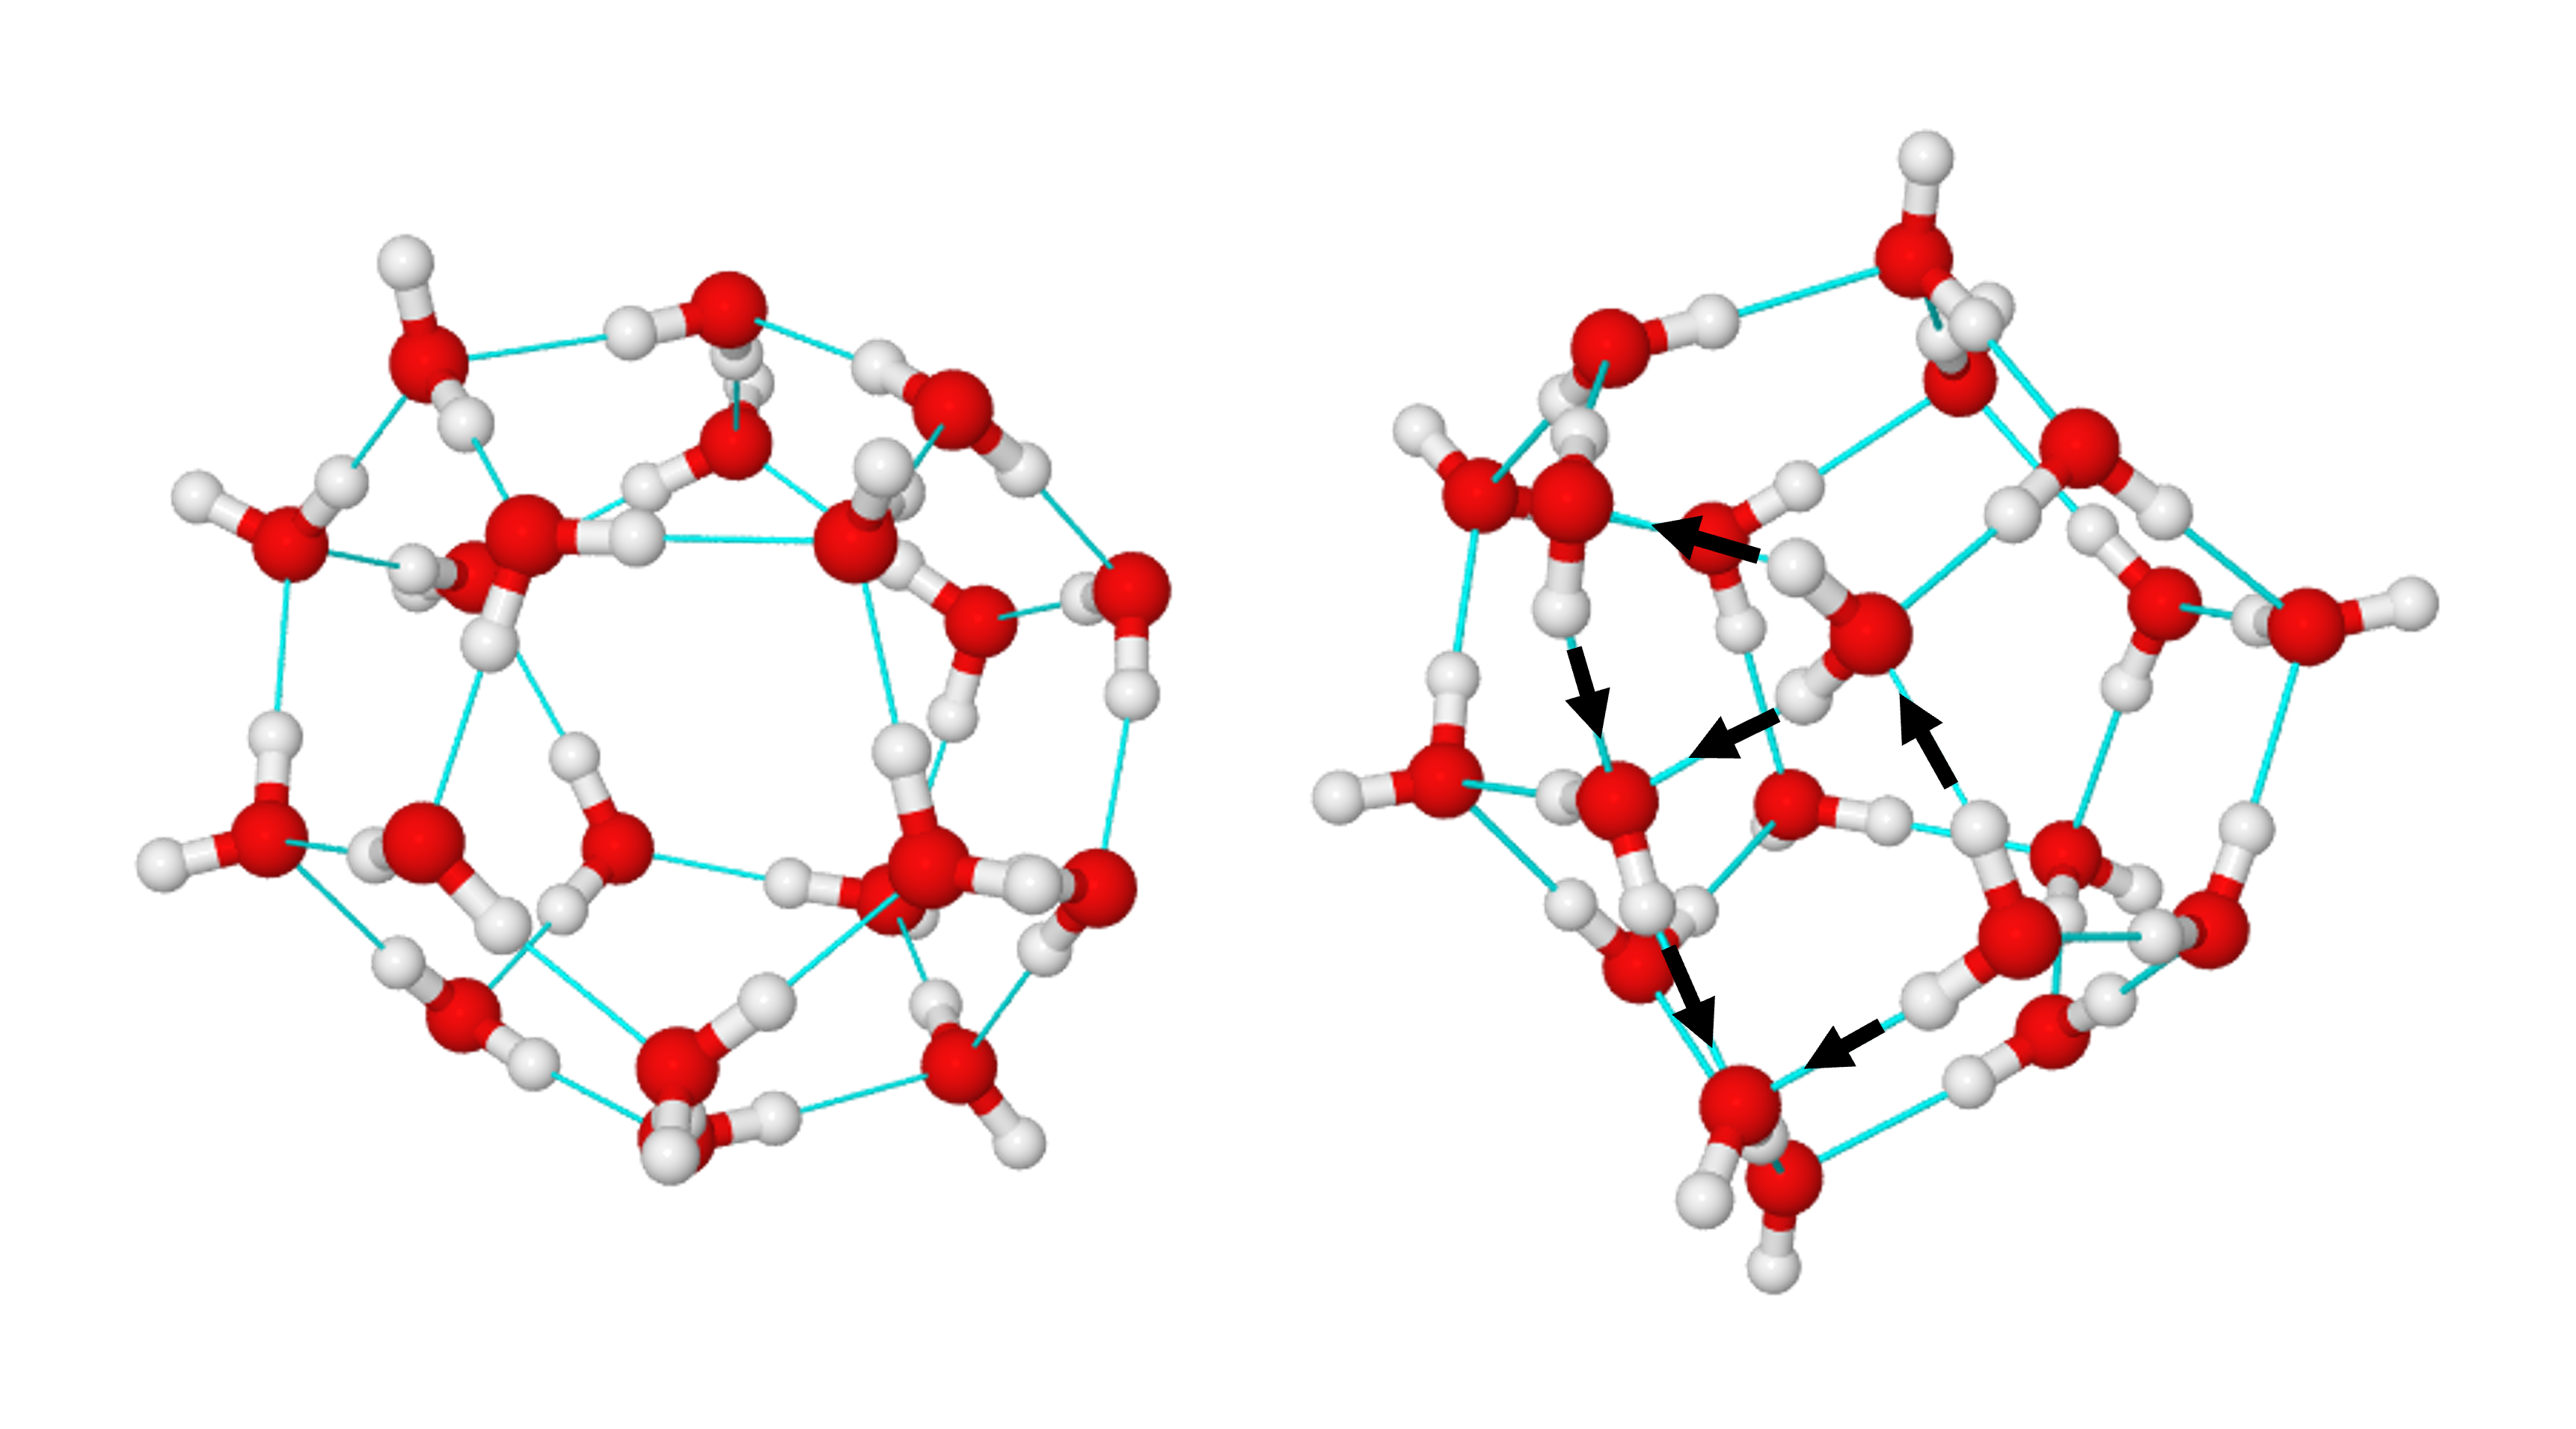
\includegraphics[width=\textwidth]{Figures/Chapter_6/clathrate_distortion_comparison.png}
\end{center}
\begin{spacing}{1.0}
\caption[Examples of a stable \ce{(H2O)_{20}} clathrate cage (left) and one of the most common defects, which occurs when a candidate clathrate structure collapses to a different hydrogen bonding arrangement. The arrows show that a free OH bridges one of the 5-membered rings in \ce{(H2O)_{20}}, resulting in fused 3- and 4-membered rings.]{Examples of a stable \ce{(H2O)_{20}} clathrate cage (left) and one of the most common defects, which occurs when a candidate clathrate structure collapses to a different hydrogen bonding arrangement. The arrows show that a free OH bridges one of the 5-membered rings in \ce{(H2O)_{20}}, resulting in fused 3- and 4-membered rings.}\label{fig:MBE_III_F3}
\end{spacing}
\end{figure}

\par Figure \ref{fig:MBE_III_F3} shows such an example of a stable cage \ce{(H2O)_{20}} structure (left) and the most common type of defect structure (right) when the cage optimizes to a different hydrogen bond topology than the regular dodecahedral cage. The arrows in Figure \ref{fig:MBE_III_F3} show that when a structure collapses, it very often does so by rotating a free OH to bridge a 5-membered ring resulting in fused 3- and 4-membered rings. We found that this same defect also regularly occurs upon optimization of microstates of the \ce{(H2O)_{24}} and \ce{(H2O)_{28}} hollow cages. This type of defect maintains a similar oxygen framework to the clathrate cages while introducing 4-coordinated water molecules not normally found in clathrate lattices. We also found that in some cases the structure collapses to an entirely different oxygen framework, usually by allowing a water molecule to move into the center of the cage and assume the structure of a “liquid-like” fully connected network.

\begin{figure}[t]
\uwsinglespace
\begin{center}
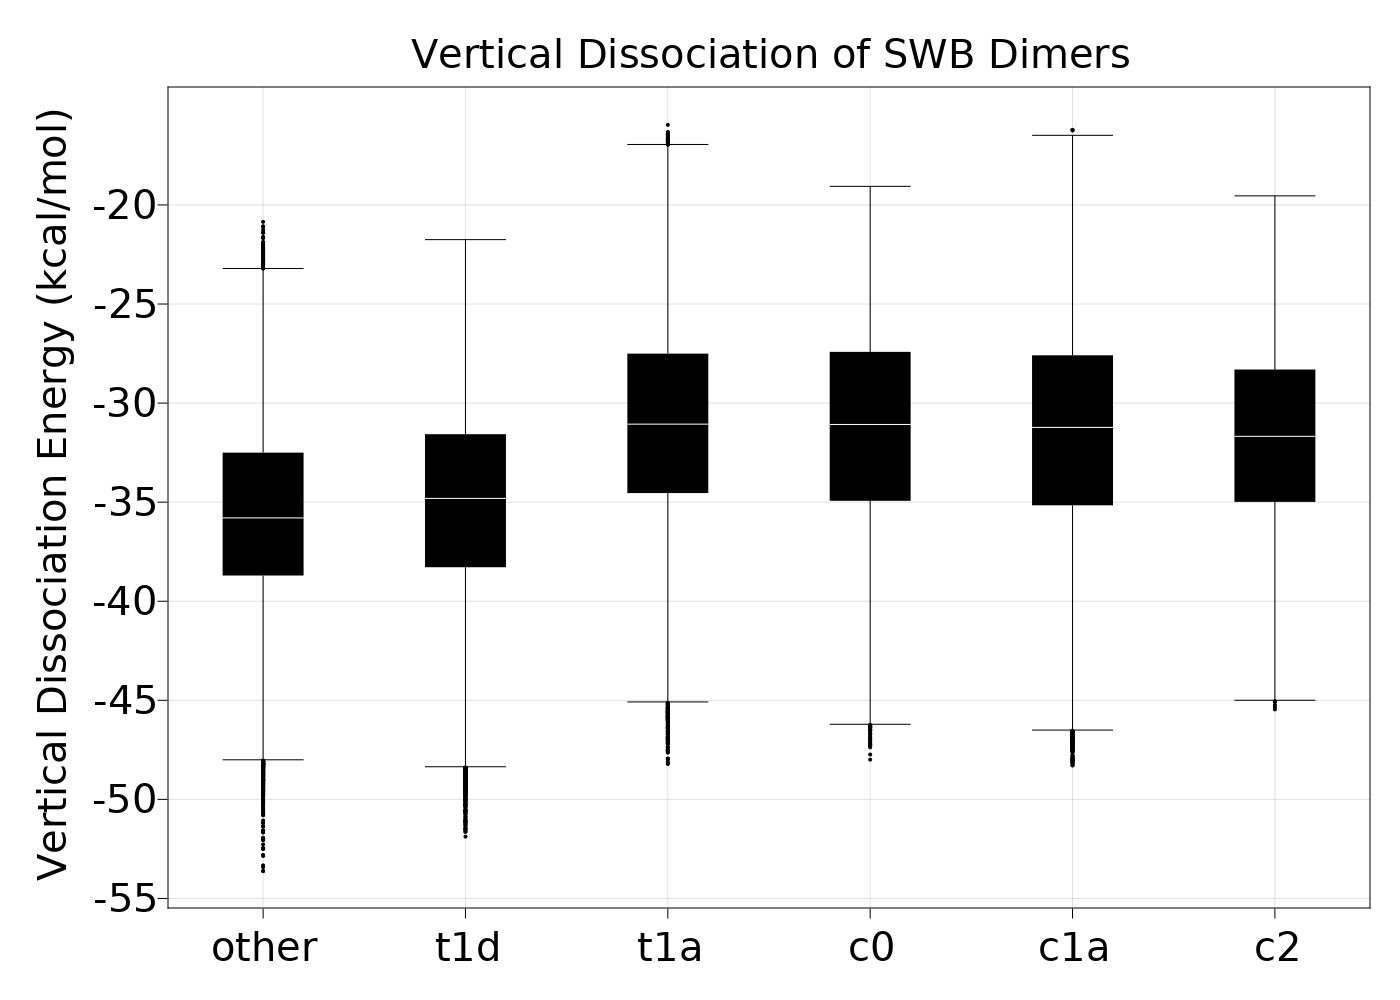
\includegraphics[width=.9\textwidth]{Figures/Chapter_6/w20_clathrate_vertical_dissociation_dimers.png}
\end{center}
\begin{spacing}{1.0}
\caption[Vertical dissociation energy (see text for details) of all dimers from all 30,026 optimized \ce{(H2O)_{20}} clathrate cages. Note that t1d dimers are about 3 kcal/mol more stable than all other types of dimers, on average, while all other SWEB dimers are similarly stable. The non-SWEB dimers present in collapsed cages are of slightly more stable than t1d dimers on average.]{Vertical dissociation energy (see text for details) of all dimers from all 30,026 optimized \ce{(H2O)_{20}} clathrate cages. Note that t1d dimers are about 3 kcal/mol more stable than all other types of dimers, on average, while all other SWEB dimers are similarly stable. The non-SWEB dimers present in collapsed cages are of slightly more stable than t1d dimers on average.}\label{fig:MBE_III_F4}
\end{spacing}
\end{figure}

\par The SWEB model provides a framework for understanding the relative stability of the cage microstates based on the relative orientation (and corresponding stability) of the individual nearest-neighbor dimers making up the polyhedral cage. In order to better quantify the relative stability of these different dimer orientations, we calculated the dimer vertical dissociation energy (DVDE) of each dimer cut out of the 30,026 optimized structures for \ce{(H2O)_{20}}. Since the SWEB model only defines dimers containing 3-coordinated water molecules, any of the non-SWEB dimers in the collapsed structures discussed above are categorized as “other” in Figure \ref{fig:MBE_III_F4}. Notice that the t1d dimers are about 3 kcal/mol more stable than any of the other SWEB dimers. This is about half the energy of a hydrogen bond on its own and the maximum number of t1d dimers are 7, 9 and 11 in \ce{(H2O)_{20}}, \ce{(H2O)_{24}}, and \ce{(H2O)_{28}}, respectively. These two facts together provide a simple way of accounting for the large, $\Tilde{}$25 kcal/mol range between the most and least stable microstates of the \ce{(H2O)_{20}} cage. That is, each t1d dimer removed has to be replaced with some other SWEB dimer, which raises the energy by about 3 kcal/mol on average for each dimer.

\begin{figure}[t]
\uwsinglespace
\begin{center}
\begin{minipage}{0.45\textwidth}
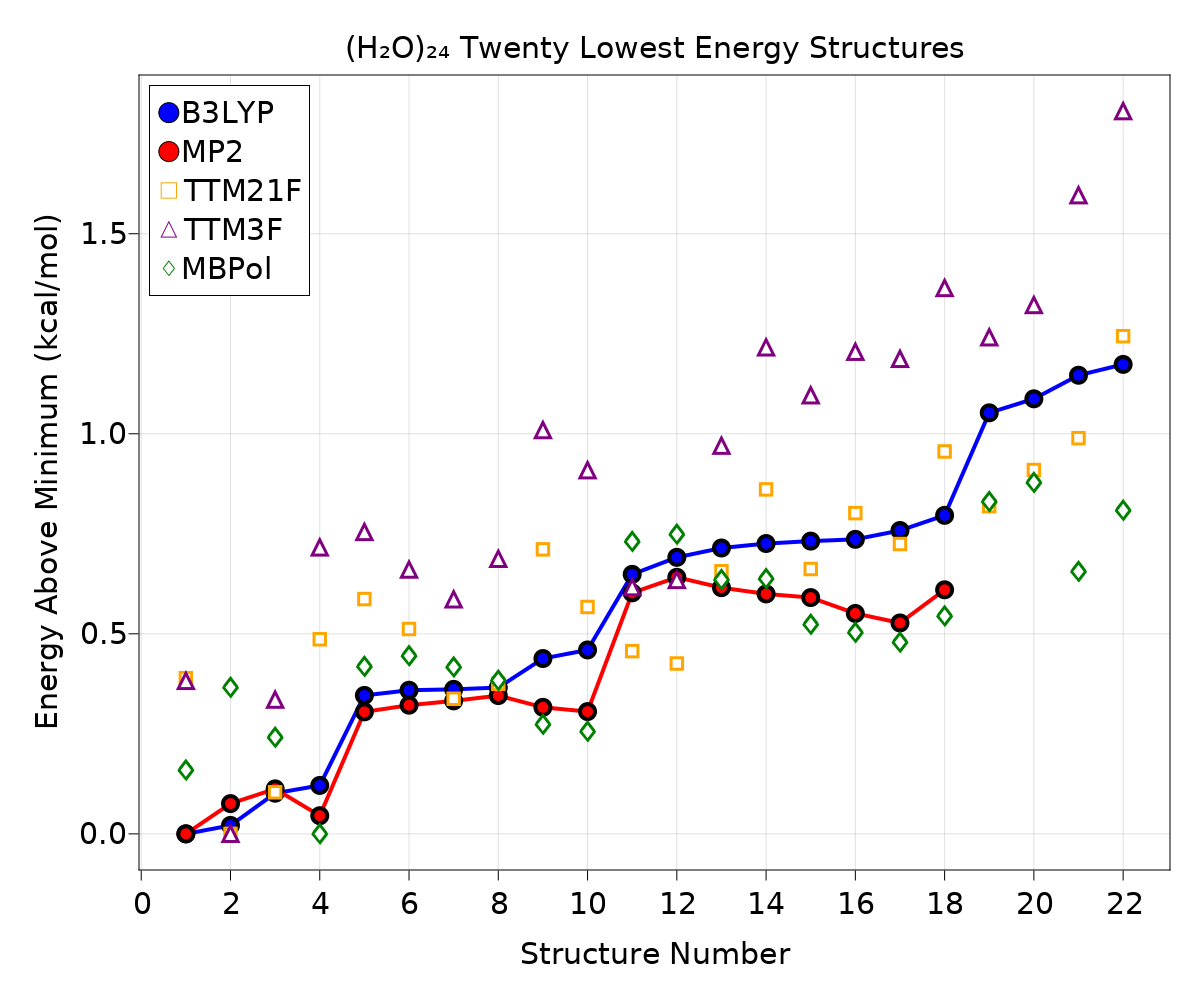
\includegraphics[width=\textwidth]{Figures/Chapter_6/w24_lowest_22_dipole_structures.png}
\end{minipage}
\begin{minipage}{0.45\textwidth}
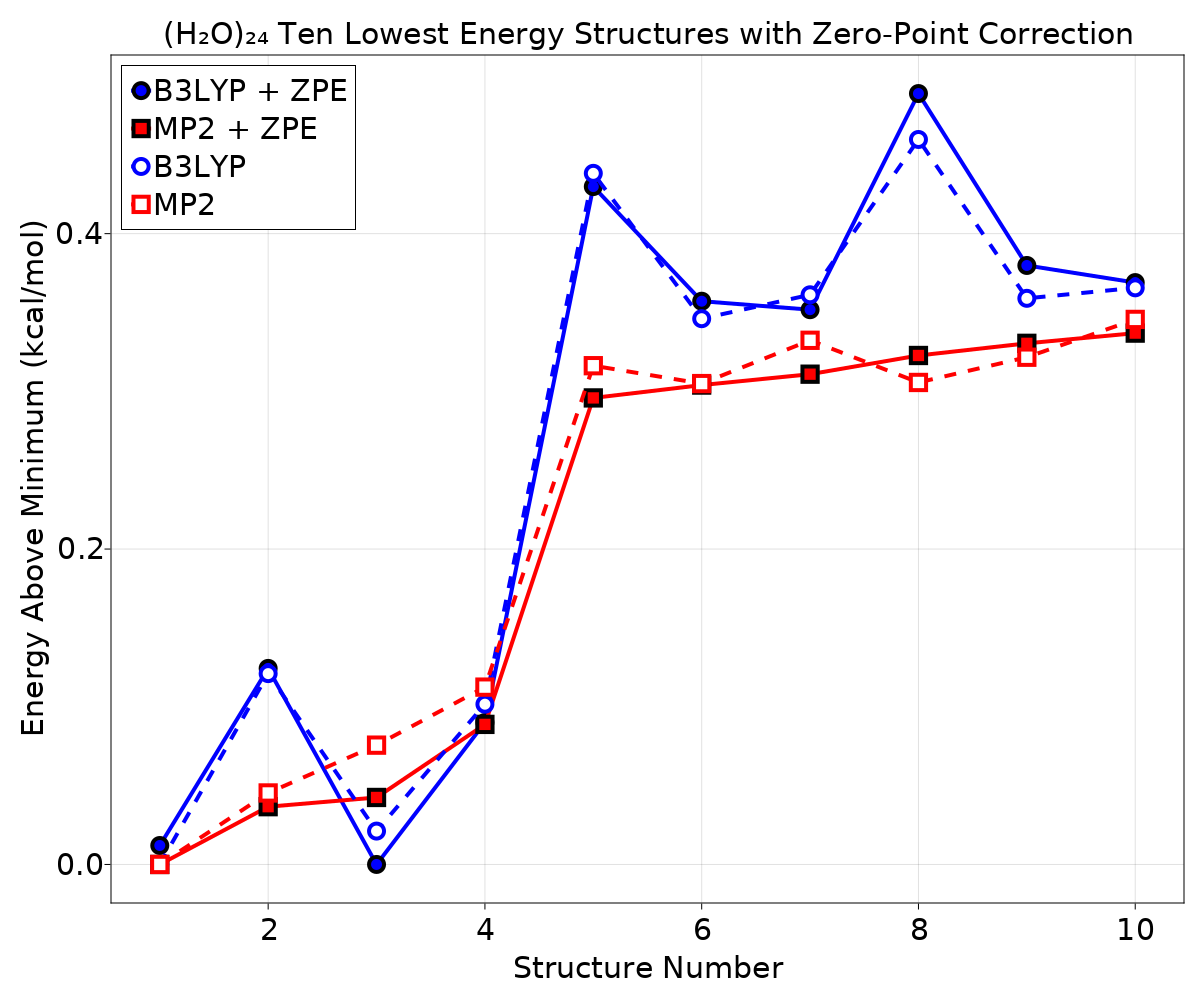
\includegraphics[width=\textwidth]{Figures/Chapter_6/w24_lowest_ten_structures_plus_zpe.png}
\end{minipage}
\end{center}
\begin{spacing}{1.0}
\caption[The left panel shows a comparison of B3LYP/TZVP and MP2/TZVP calculations of the 22 lowest \ce{(H2O)_{24}} structures with minimal dipoles. Calculations with TTM2.1-F, TTM3-F, and MB-Pol are also shown. The right panel shows the effect of harmonic zero-point energy correction on these ten lowest structures.]{The left panel shows a comparison of B3LYP/TZVP and MP2/TZVP calculations of the 22 lowest \ce{(H2O)_{24}} structures with minimal dipoles. Calculations with TTM2.1-F, TTM3-F, and MB-Pol are also shown. The right panel shows the effect of harmonic zero-point energy correction on these ten lowest structures.}\label{fig:MBE_III_F6}
\end{spacing}
\end{figure}

\par Previous work by Tokmachev using semi-empirical calculations showed that the highest-energy \ce{(H2O)_{20}} microstate is \textapprox 30 kcal/mol higher in energy than the lowest energy one. We find similar results with TTM2.1-F and MB-Pol potentials, both of which have proven to be accurate in predicting the binding energies of water clusters compared to high level ab-initio results. This surprisingly large difference in energy between the lowest and highest energy structures further emphasizes the importance of hydrogen-bonding cooperativity in water. Hydrogen-bonding cooperativity is usually described as the percentage of the many-body contributions to the binding energy (that is, contributions that depend on more than two monomers).\autocite{xantheas_cooperativity_2000}

\begin{figure}[t]
\uwsinglespace
\begin{center}
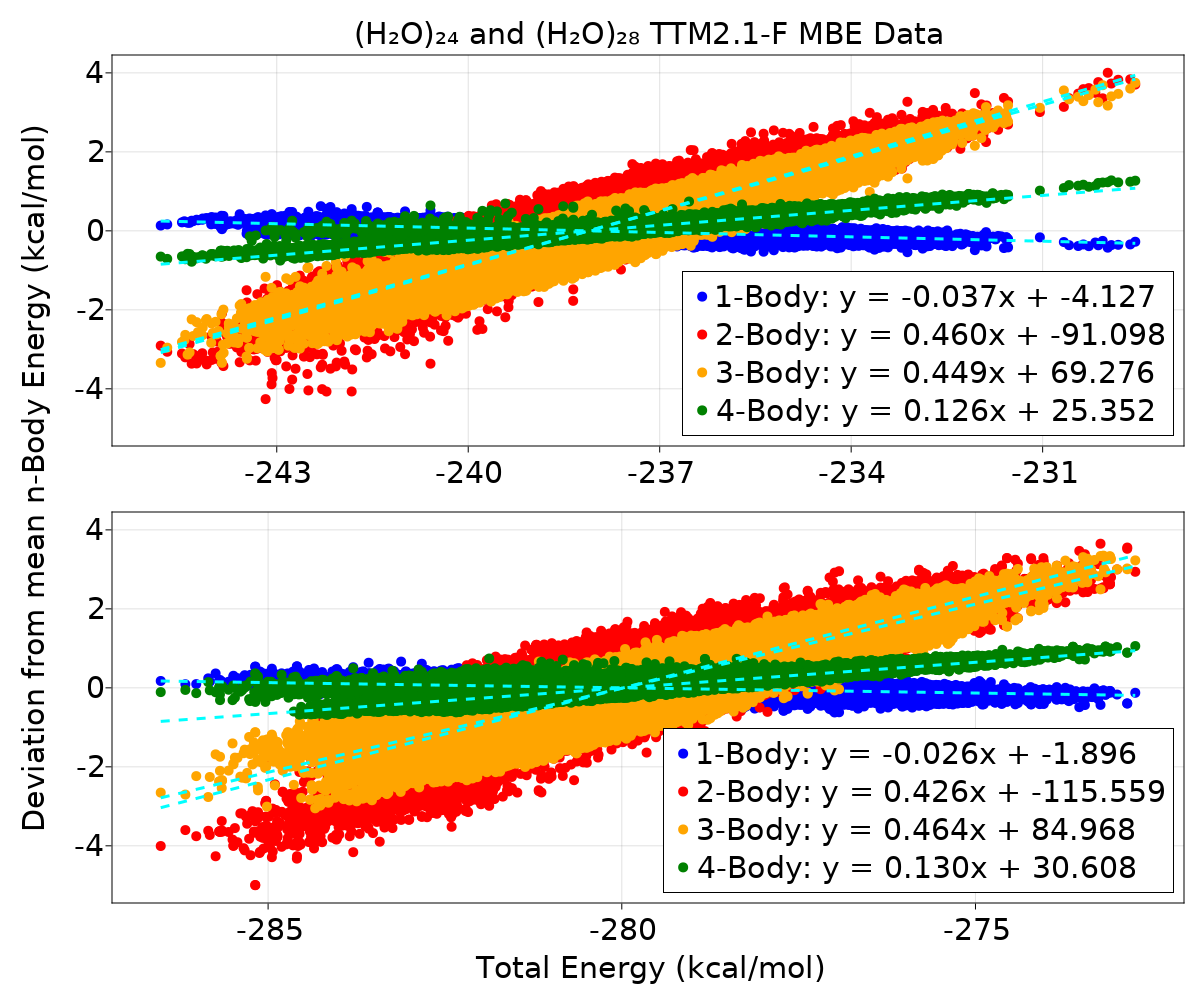
\includegraphics[width=.8\textwidth]{Figures/Chapter_6/w24_and_w28_mbe_ttm21f_deviation.png}
\end{center}
\begin{spacing}{1.0}
\caption[Panels for \ce{(H2O)_{24}} (top) and \ce{(H2O)_{28}} (bottom), showing the deviation of each many-body term $E_{nB}$ from the average of the same many-body term, $\langle E_nB\rangle$, plotted against the total energy for a cluster. Notice that the slope of each line is the percentage contribution to the binding energy.]{Panels for \ce{(H2O)_{24}} (top) and \ce{(H2O)_{28}} (bottom), showing the deviation of each many-body term $E_{nB}$ from the average of the same many-body term, $\langle E_nB\rangle$, plotted against the total energy for a cluster. Notice that the slope of each line is the percentage contribution to the binding energy.}\label{fig:MBE_III_F5}
\end{spacing}
\end{figure}

\par We have performed the MBE analysis for all stable microstates with k = 7 – 9 (for \ce{(H2O)_{24}}) and k = 9 – 11 (for \ce{(H2O)_{28}}) t1d dimers, respectively. These calculations provide a way to index the relative importance of the individual 1-, 2-, 3-, and 4-body energy terms for the family of hollow cage water structures. Figures \ref{fig:MBE_III_F5}a and \ref{fig:MBE_III_F5}b show each many-body term up to 4-body plotted as a difference from the mean of each term over all stable structures within each family of structures using the TTM2.1-F potential. The slope of each line can be interpreted as the correlation of each many-body term to the average binding energy within the family whereas the y-intercept is the average of that many-body term over the family. This plot reveals the sensitivity of an entire oxygen framework family to the cooperativity of hydrogen-bonding. The fact that each term varies linearly with energy shows that many-body effects vary consistently within the oxygen framework family. To the best of our knowledge this trend has not been reported before and could have implications in explaining the relative stability of different ice phases and/or different families of water cluster isomers.

\par Additionally, the results of Figure \ref{fig:MBE_III_F5} demonstrate that many-body effects are quite important in stabilizing these structures in which every water is on the surface of the polyhedral water cluster. It would be of interest to construct similar plots for many different oxygen families so that one can attempt to correlate these slopes to structural descriptors of the underlying hydrogen bonding networks. This type of analysis is now possible using the large database of water cluster structures, which has been recently published by some of us.\autocite{rakshit_atlas_2019} One would expect that a larger slope for the 3- and 4-body terms (and hence a smaller 2-body slope) will be correlated with the number of homodromic rings in the network, as these have been shown to maximize many-body effects.\autocite{xantheas_ab_1994,xantheas_cooperativity_2000} However, the structural characteristics which are anti-correlated to the many-body stabilization are less well understood despite their importance in aqueous systems containing ions.\autocite{heindel_many-body_2021,mherman_many-body_2021}

\subsection{Low energy isomers of \ce{(H2O)_{24}} and \ce{(H2O)_{28}} hollow cages}

\par Finding either the global or even the putative minimum of a medium to large molecular cluster on a complex multi-dimenstional PES such as the one characteristic of the hollow water cages is a challenging task.\autocite{wales_exploring_2018} Since the naturally occurring clathrate lattices are composed of cages of varying size, each of which have many possible hydrogen bonding arrangements, choosing the placement of hydrogen atoms in a clathrate lattice so that each corresponds to a low energy network is quite challenging. A thorough analysis locating low energy isomers of the \ce{(H2O)_{20}} dodecahedral cage has been previously reported.\autocite{xantheas_lowlying_2012} We aim to locate the lowest energy isomers of \ce{(H2O)_{24}} in a similar manner. Starting from these low energy cage networks, the low-energy candidates for the full sI lattice can be constructed.\autocite{yoo_low-energy_2009}

\begin{figure}[t]
\uwsinglespace
\begin{center}
\begin{minipage}{0.45\textwidth}
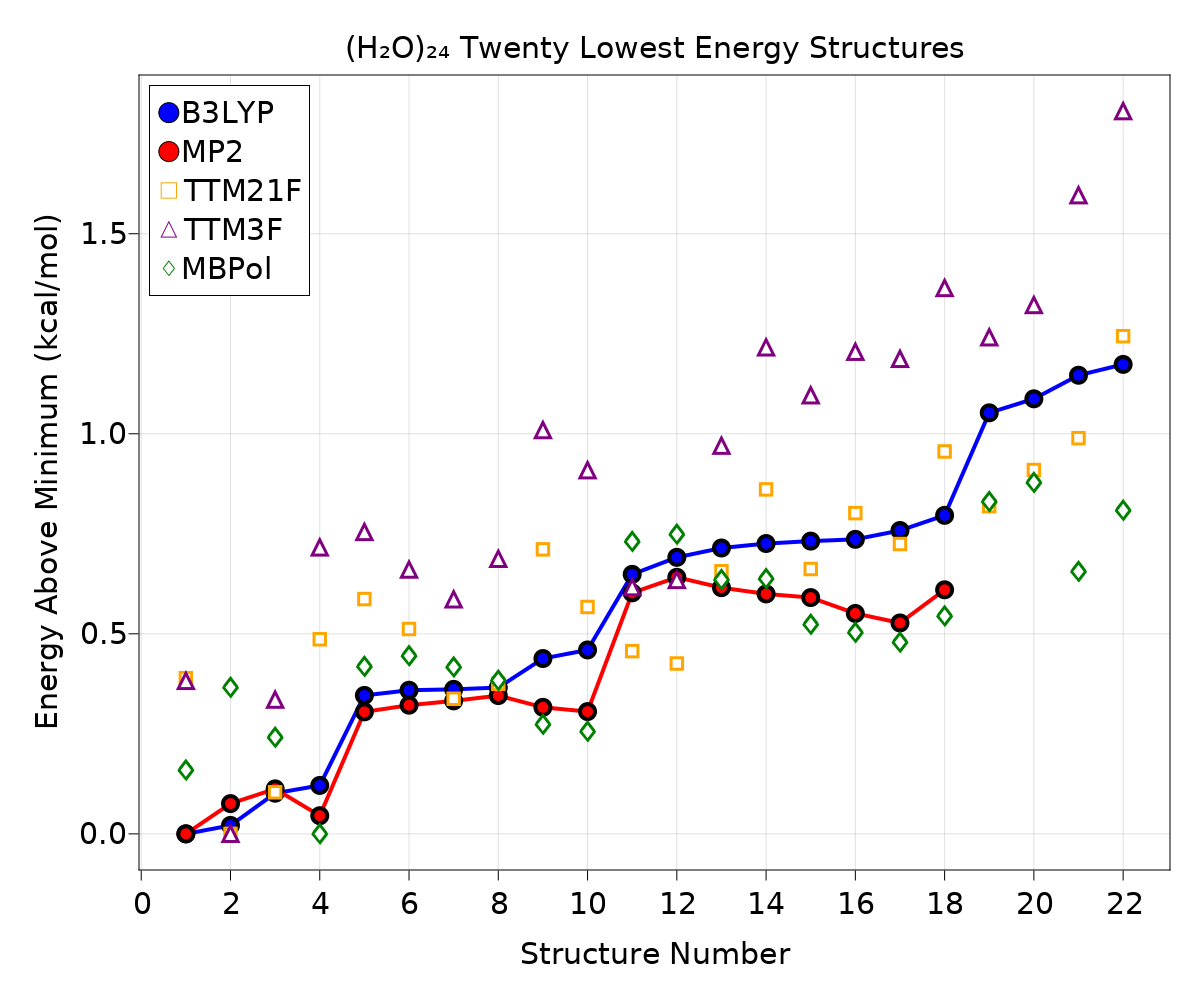
\includegraphics[width=\textwidth]{Figures/Chapter_6/w24_lowest_22_dipole_structures.png}
\end{minipage}
\begin{minipage}{0.45\textwidth}
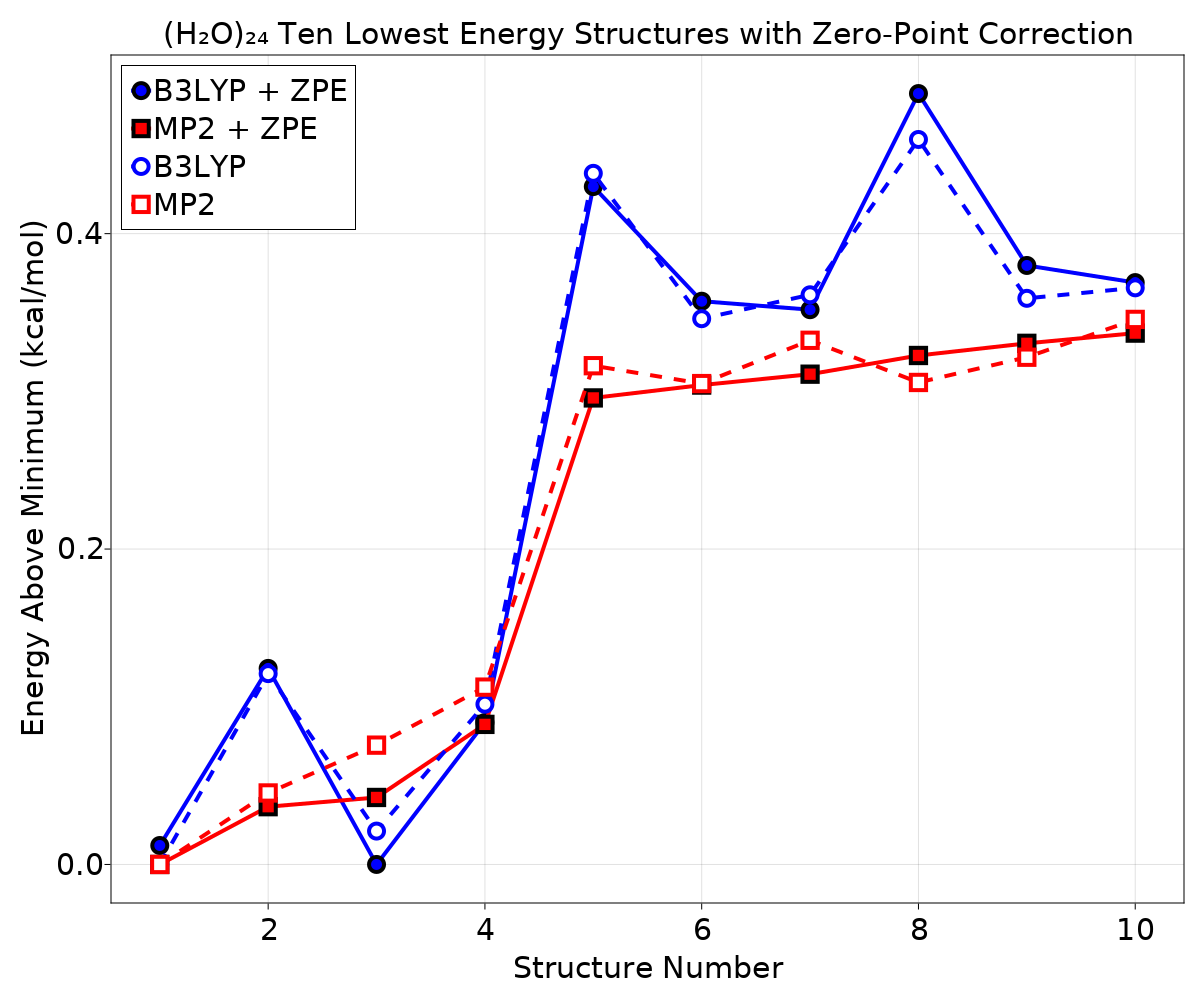
\includegraphics[width=\textwidth]{Figures/Chapter_6/w24_lowest_ten_structures_plus_zpe.png}
\end{minipage}
\end{center}
\begin{spacing}{1.0}
\caption[The left panel shows a comparison of B3LYP/TZVP and MP2/TZVP calculations of the 22 lowest \ce{(H2O)_{24}} structures with minimal dipoles. Calculations with TTM2.1-F, TTM3-F, and MB-Pol are also shown. The right panel shows the effect of harmonic zero-point energy correction on these ten lowest structures.]{The left panel shows a comparison of B3LYP/TZVP and MP2/TZVP calculations of the 22 lowest \ce{(H2O)_{24}} structures with minimal dipoles. Calculations with TTM2.1-F, TTM3-F, and MB-Pol are also shown. The right panel shows the effect of harmonic zero-point energy correction on these ten lowest structures.}\label{fig:MBE_III_F6}
\end{spacing}
\end{figure}

\par Figure \ref{fig:MBE_III_F6}a shows the binding energies of twenty \ce{(H2O)_{24}} isomers calculated with B3LYP/TZVP and MP2/TZVP, including BSSE correction. For comparison, Figure \ref{fig:MBE_III_F6}a shows the energy of the same structures optimized with TTM2.1-F, TTM3-F\autocite{fanourgakis_development_2008}, and MB-Pol. All of these structures have the maximum of nine t1d dimers. There is an interesting partitioning of the structures into closely separated levels. Figure \ref{fig:MBE_III_F6}b expands on Figure \ref{fig:MBE_III_F6}a by including harmonic zero-point energy (ZPE) corrections at the B3LYP/TZVP and MP2/TZVP level. Interestingly, ZPE has almost no effect on the relative energy difference of each structure. Figure \ref{fig:MBE_III_F6}b makes it clear that the lowest energy structures are split into two levels where each isomer has approximately the same energy.

\begin{figure}[t]
\uwsinglespace
\begin{center}
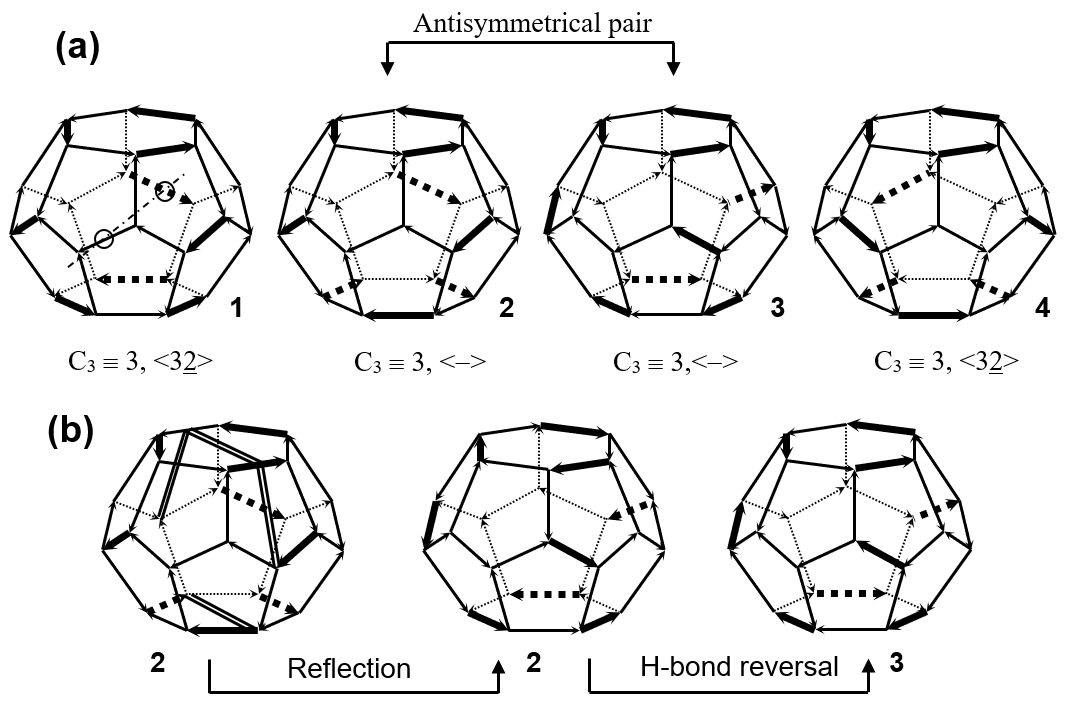
\includegraphics[width=.9\textwidth]{Figures/Chapter_6/symmetry_operations.png}
\end{center}
\begin{spacing}{1.0}
\caption[(a) Four lowest energy configurations of \ce{(H2O)_{24}} polyhedron. The arrows indicate the direction of the hydrogen bond: from the proton donor to the acceptor. In configurations 1 and 4, the lateral antisymmetry axes 2 (circles) pass through one t1d-bond that are shown with bold lines. (b) The antisymmetry transformation (anti-reflection in plane) which relates antipode configurations 2 and 3. This emphasizes the connection between near-symmetry and low-energy configurations.]{(a) Four lowest energy configurations of \ce{(H2O)_{24}} polyhedron. The arrows indicate the direction of the hydrogen bond: from the proton donor to the acceptor. In configurations 1 and 4, the lateral antisymmetry axes 2 (circles) pass through one t1d-bond that are shown with bold lines. (b) The antisymmetry transformation (anti-reflection in plane) which relates antipode configurations 2 and 3. This emphasizes the connection between near-symmetry and low-energy configurations.}\label{fig:MBE_III_F7}
\end{spacing}
\end{figure}

\par When analyzing the structure of the lowest energy configurations of the T cage, \ce{(H2O)_{24}}, it was found that the four most stable configurations are rather symmetrical (Figure \ref{fig:MBE_III_F6}). The upper and bottom H-bonded hexagons and the broken equatorial cycle are homodromic. The remaining oblique-vertical H-bonds are oriented alternately. All four configurations have 3-fold symmetry axes (vertical). The Schoenflis designation and the international symmetry designation are used here. The latter is more convenient for extended symmetry, which is shown in parentheses. The most stable molecular structures are often symmetrical or nearly symmetrical\autocite{wales_symmetry_1998}.

\par Another interesting feature is that two of the \ce{(H2O)_{24}} configurations are antisymmetric, and the remaining two form a pair of antipode configurations (Fig. \ref{fig:MBE_III_F6}). The location of one of the three 2-fold antisymmetry axes of the first structure is shown by a dashed line passing through two circles. After rotation by 180 degrees, the direction of the bonds in the hexagonal cycles and the equatorial cycle changes to the opposite direction. But after hydrogen-bond-reversal, the direction of the cycles coincides with the original one. The same happens with the rest of the inclined-vertical bonds. To verify that configurations 2 and 3 form an antisymmetric pair, it is necessary to reflect configuration 2 in the plane indicated in the figure (double lines) and then change the direction of all hydrogen bonds.

\subsection{Dipole Moments of Low-Energy Cages}

\begin{figure}[t]
\uwsinglespace
\begin{center}
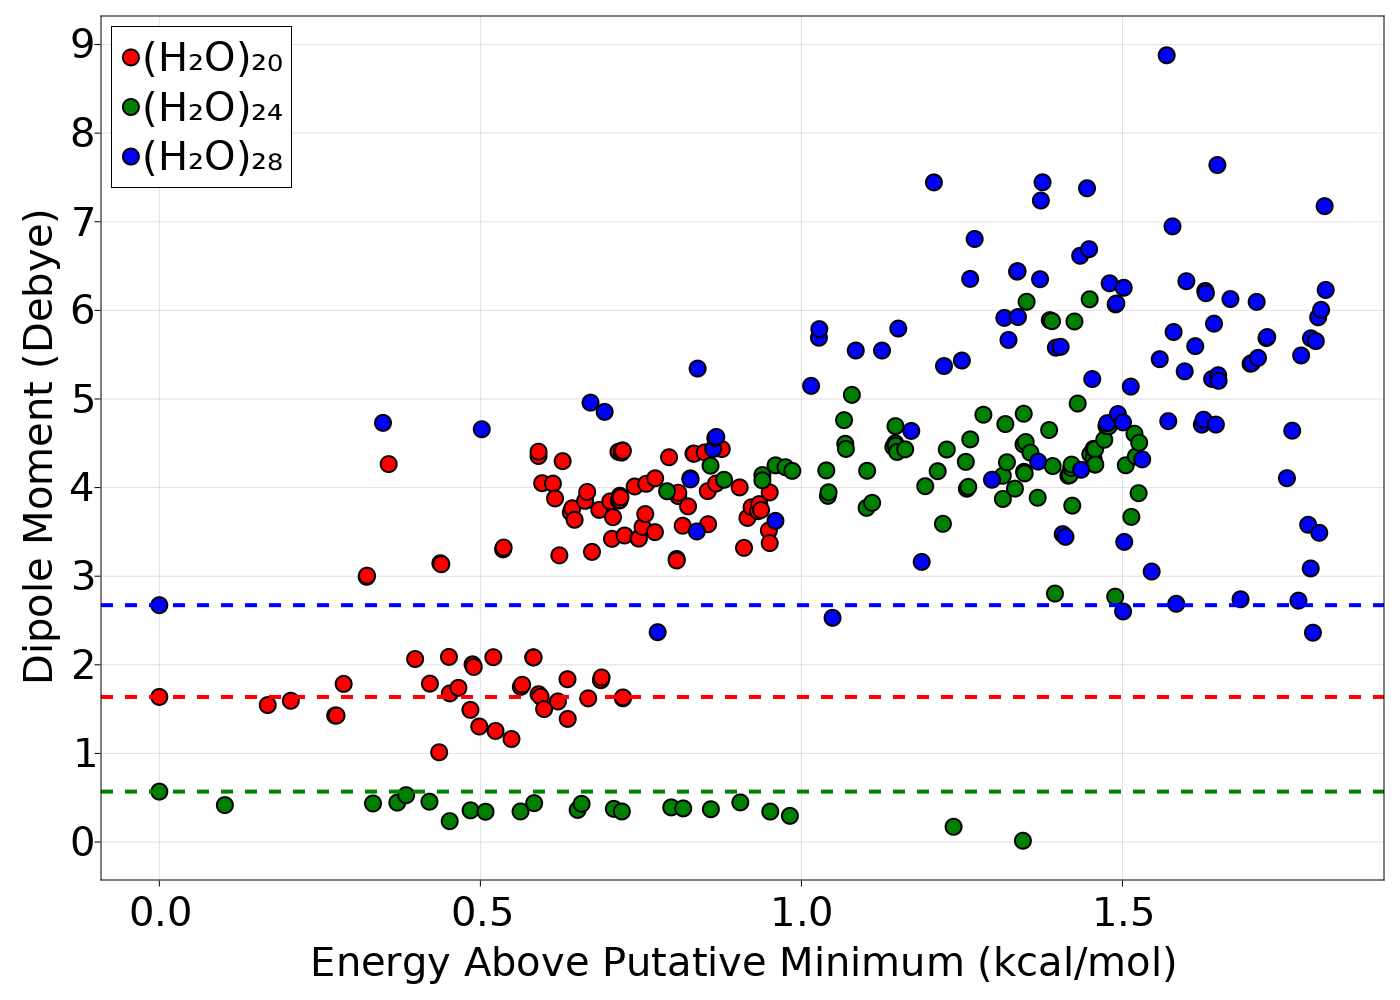
\includegraphics[width=.85\textwidth]{Figures/Chapter_6/all_clathrate_cages_dipole_vs_energy.png}
\end{center}
\begin{spacing}{1.0}
\caption[Comparison of the dipole moment of the 100 lowest energy structures of \ce{(H2O)_{20}}, \ce{(H2O)_{24}}, and \ce{(H2O)_{28}} to the energy of each configuration. The binding energies are shown as the energy difference between each structure and the lowest energy cage of that size. All data in this figure come from the TTM2.1-F potential. Dashed lines show the dipole moment of the putative minimum structure, which always corresponds to one of the lowest energy configurations.]{Comparison of the dipole moment of the 100 lowest energy structures of \ce{(H2O)_{20}}, \ce{(H2O)_{24}}, and \ce{(H2O)_{28}} to the energy of each configuration. The binding energies are shown as the energy difference between each structure and the lowest energy cage of that size. All data in this figure come from the TTM2.1-F potential. Dashed lines show the dipole moment of the putative minimum structure, which always corresponds to one of the lowest energy configurations.}\label{fig:MBE_III_F8}
\end{spacing}
\end{figure}

\par When constructing a crystal structure from the constituent hollow cages, it is desirable that the dipoles of the individual cages must be arranged in such a way as to cancel the total dipole moment. This might lead to the hypothesis that the cages with the smallest dipole moment may also be candidates for low-energy isomers. In fact, this has been already reported for the \ce{(H2O)_{20}} cages in past work.\autocite{kirov_identifying_2008} The dipole moment of the 100 lowest energy configurations of the \ce{(H2O)_{20}}, \ce{(H2O)_{24}}, and \ce{(H2O)_{28}} cages against the binding energy of each cage relative to the lowest energy configuration of each cage is shown in Figure \ref{fig:MBE_III_F8}. For the \ce{(H2O)_{20}} and \ce{(H2O)_{24}} cages, there exist islands of isomers which have approximately the same dipole moment and correspondingly low energies, whereas for the \ce{(H2O)_{28}} cage there is no grouping of configurations with approximately the same dipole moment. The dipole moment is clearly not a perfect descriptor of the binding energy, but the dipole and energy are clearly positively correlated, especially in \ce{(H2O)_{28}} where the clusters have quite different dipole moments.

\par One should intuitively expect that these cages, and in addition water clusters in general, will be more strongly bound when minimizing the dipole moment of the cluster. This is because the more that the electric field produced by each molecule is quenched, the stronger the interactions between molecules ought to be. Since there are very few hollow cages with symmetry, almost all cages have a nonzero dipole moment. This means that the crystal structure will likely contain a mix of many possible cage configurations, even ones that are somewhat higher in energy, to prevent a net-dipole from accumulating in the crystal structure. It could be interesting to simulate the formation of clathrate crystal lattices and see which cages are naturally formed, especially focusing on how the energy distribution of cages in a crystal lattice compares to the energy distribution of isolated cages.

\section{Conclusions}

\par We have explicitly enumerated all non-isomorphic hydrogen-bonding arrangements of the \ce{(H2O)_{20}}, \ce{(H2O)_{24}}, and \ce{(H2O)_{28}} cages making up the sI and sII clathrate hydrate crystal structures. We have optimized all \ce{(H2O)_{20}} cages using the TTM2.1-F and MB-Pol classical water potentials showing that about 90\% of possible hydrogen-bonding arrangements correspond to actual local minima. We have shown that the arrangements most likely to collapse to non-hollow, lower energy, liquid-like structures are those with less than the maximum number of t1d dimers for each case. For the \ce{(H2O)_{24}} and \ce{(H2O)_{28}} cages we optimized structures containing 7- 9 and 9 - 11 t1d dimers, respectively. About 90\% of these structures were found to correspond to true local minima, indicating that if all possible cage microstates were to be optimized, an even smaller percentage would produce local minima. The least stable hydrogen-bonding arrangement of \ce{(H2O)_{20}} is about 28 kcal/mol higher in energy than the most stable one with both the TTM2.1-F and MB-Pol potentials. The range of energies for \ce{(H2O)_{24}} and \ce{(H2O)_{28}} would be even larger, however we did not optimize most of the very high energy structures due to the overwhelmingly large number of arrangements of these larger water clusters.

\par For the three hollow water cages considered in this study we have also provided estimates of the residual entropy based on the number of possible hydrogen-bonding arrangements of these cages including isomorphic ones. The residual entropy of each cage agrees very well with the estimate based on a simple, combinatorial counting approach introduced by Pauling for ice polymorphs. We also note that the residual entropy is related to the wide energy range spanned by these hydrogen-bonding arrangements since it reflects how much free energy gets frozen into a crystal lattice. Without experimental measurements of the residual entropy of these lattices, however, it is very difficult to know how many of these hydrogen-bonding arrangements would appear in the actual crystal structure of a clathrate hydrate.

\par Finally, the fact that these hundreds of thousands to tens of millions of structures differ only in the arrangement of hydrogen bonds makes them intriguing systems to analyze the subtleties of hydrogen-bonding interactions. We have studied these interactions by computing the many-body expansion up to the 4-body term with the TTM2.1-F classical water potential. We show that each of the many-body terms varies linearly with the binding energy of each cluster in the \ce{(H2O)_{20}}, \ce{(H2O)_{24}}, and \ce{(H2O)_{28}} cages. The slopes of each many-body term within an oxygen family provide a measure of the hydrogen-bond cooperativity within an oxygen atom framework. For instance, the 2-body and 3-body terms have similar slopes with respect to the total energy for each of these cages. This indicates the relative importance of hydrogen bond cooperativity within these cages which entirely consist of fused rings.

\chapter{Molecular Dynamics Driven by the Many-Body Expansion (MBE-MD)}
\label{ch:MBE_MD}

\section{Introduction}

\par Molecular dynamics (MD) is one of the most common and powerful tools used for studying a wide range of properties of molecular systems.\autocite{bankura_hydration_2013,bernardi_enhanced_2015,durrant_molecular_2011,hospital_molecular_2015,probst_molecular_1985} It is effective as a means for generating ensembles, as well as characterizing the dynamic response of systems. As with many theoretical tools, MD suffers from the persistent trade-off between computational cost and accuracy. The source of this problem in MD simulations arises almost entirely from the choice of potential energy surface (PES) used to generate the energies and forces between atoms. Ideally, one would be able to use highly accurate electronic structure methods, either single reference, such as Coupled Cluster with singles, doubles, and perturbative triple excitations (CCSD(T)),\autocite{bartlett_coupled-cluster_1989} or multi-reference based ones, such as MCSCF\autocite{schmidt_construction_1998}, MRCI\autocite{werner_selfconsistent_1982}, MRCC\autocite{mukherjee_linked-cluster_1986}, CASPT2\autocite{finley_multi-state_1998} or DMRG.\autocite{schollwock_density-matrix_2005} These calculations are, however, far too expensive (formally scaling as $N^a$, where $a \geq 6$) to be used for any practical MD simulations of realistic systems.

\par The scalability issue has resulted in two paradigms for generating the forces in MD simulations. The first paradigm, commonly known as a molecular mechanics (MM)\autocite{karplus_molecular_2005,karplus_molecular_2002,karplus_molecular_1990,rappe_uff_1992,engler_critical_1973,still_semianalytical_1990} approach, is to strip the electrons and approximate the energies and/or forces using closed-form equations based on functions that are deemed appropriate to describe the underlying interactions such as the Lennard-Jones potential or simple bond, angle, and dihedral potentials. The second paradigm, commonly known as ab initio or Born-Oppenheimer molecular dynamics (AIMD/BOMD),\autocite{car_unified_1985,barnett_born-oppenheimer_1993,worth_beyond_2004,li_ab_2005,tuckerman_ab_1996} is to retain the electronic degrees of freedom and generate the energies and forces from a relatively more affordable electronic structure method, such as density functional theory (DFT). The most well-known implementation of this paradigm is Car-Parrinello dynamics.\autocite{car_unified_1985} Each of these paradigms have distinct advantages and disadvantages, which we will briefly outline in order to provide the context of why our proposed MBE-MD implementation aims at getting the best of both worlds.

\par The simplest types of MM force fields describe the energy of a molecule in terms of bond distances, angles, and dihedral angles. These potential functions are extremely fast to evaluate but they are very crude approximations of the underlying intermolecular interactions and they do not contain descriptions of electrons. The field has evolved over the years from the simpler to more sophisticated descriptions of the various pieces of the interactions while at the same time improving their scalability and accuracy by explicitly fitting to high-level electronic structure calculations. For example, this approach has resulted in ab-initio based water potentials such as MB-Pol\autocite{babin_toward_2012,babin_development_2013,babin_development_2014,medders_development_2014}, WHBB\autocite{wang_full-dimensional_2009,wang_towards_2010,wang_flexible_2011}, MB-UCB\autocite{das_development_2019} and the Thole-type family of potentials.\autocite{fanourgakis_flexible_2006,fanourgakis_development_2008,burnham_development_2002} There are obviously numerous drawbacks of the MM paradigm; in short, these ab-initio based potentials generally suffer from a lack of universality and transferability. For example, even though one can fit very accurate potentials to often tens of thousands of electronic structure calculations, these are only applicable to a specific system, and they are not transferable. On the other hand, the relatively simple force fields that are more general are almost never quantitatively accurate, because it is just not possible to distill the salient features of a wide range of intermolecular interactions requiring formal quantum mechanical descriptions into simple functional forms.

\par The AIMD/BOMD paradigm naturally avoids problems related to generality because the approximations used to solve the electronic Schrodinger equation, such as for example Density Functional Theory (DFT) are, in principle, valid for any system. This means that one can easily study a family of similar systems with AIMD, where that could be quite difficult with MM. The major drawback lies in the large number of energy and gradient evaluations that are needed to propagate the dynamics, and this restricts the choices of used electronic structure methods to the ones with lower scaling, typically DFT and more recently MP2.\autocite{kuhne_cp2k_2020} An additional complexity is associated with the choice of the DFT functionals\autocite{perdew_density_2001}, and the realization that a “universal” density functional that accurately describes a wide range and different classes of interactions has yet to be developed. Nonetheless, AIMD generally results in simulations that are more trustworthy and accurate for a variety of systems than can be achieved with simple MM approaches. Noted exceptions are classical force fields that are parametrized for a specific system such as the family of TTM, MB-pol, HBB2 or MB-UCB potentials for water.\autocite{babin_development_2013,babin_development_2014,medders_development_2014,das_development_2019,fanourgakis_bend_2006,fanourgakis_development_2008,burnham_development_2002} Even so, one would ideally like to be able to use highly correlated, more accurate but higher scaling methods, such as CCSD(T), rather than DFT. However, as of yet, this has not been possible for all but the simplest molecular systems (typically with less than 30 atoms) and even for those, one is restricted to geometry optimizations and harmonic frequency calculations with no reported examples of converged dynamics calculations.

\par Clearly, the ideal situation would be to have all of the generality and accuracy of ab initio methods combined with the reduced scalability of MM methods. It has been previously proposed\autocite{herbert_fantasy_2019} that the many-body expansion (MBE) is a viable approach to reap the benefits of both of these paradigms. Indeed, the MBE or its variants have been used successfully as the basis for the development of the aforementioned highly accurate water potentials.\autocite{babin_development_2013,babin_development_2014,medders_development_2014,das_development_2019,fanourgakis_bend_2006,fanourgakis_development_2008,burnham_development_2002} The MBE has also been successful as a way of mixing multiple electronic structure methods to allow for benchmarking and geometry optimizations of large gas-phase clusters.\autocite{bates_development_2011,bates_efficient_2011,howard_n-body_2013} A comprehensive review of the pros and cons of the many different fragment-based quantum chemistry methods has been recently summarized by Herbert.\autocite{herbert_fantasy_2019}

\par One of the most useful features of the MBE in terms of its applicability to MD simulations is the tremendous flexibility in the level of theory that can be used at different orders of the MBE. Past work shows that highly correlated methods and large basis sets only need to be used for the 1- and 2-body parts of the MBE, while the 3-body and higher-order terms are nearly saturated both in terms of electronic structure method and basis when at the  HF/aug-cc-pVDZ level of theory.\autocite{heindel_many-body_2020} Another advantage of the MBE in driving AIMD simulations is the possibility of using purely classical descriptions for the many-body terms, which would make the most expensive part of the MBE (in terms of both system size and number of fragments) essentially free.

\par There have been previous reports of AIMD simulations driven by the MBE,\autocite{liu_structure_2017,liu_hydrogen-bond_2018,willow_ab_2015,he_second-order_2012} which employed either the electrostatically-embedded (EE) formalism proposed by Dahlke and Truhlar,\autocite{dahlke_electrostatically_2007} the embedded-fragment method,\autocite{willow_ab_2015} or the field-adapted adjustable density matrix assembler approach of Exner and Mezey.\autocite{exner_field-adapted_2004} Another approach to circumvent the poor scaling of electronic structure is the molecular tailoring approach (MTA).\autocite{sahu_molecular_2014} In this approach, one splits the system into many different overlapping sub-fragments, which are often larger than just a single molecule. Any electronic structure property of interest can then be calculated on these fragments and recombined via the inclusion-exclusion principle to approximate properties of the full system. The MTA can even be applied to large biomolecules, by choosing fragments which break covalent bonds.\autocite{ganesh_molecular_2006} One of the earliest, and most influential, fragmentation schemes is the molecular fractionation with conjugate caps (MFCC), which decomposes large molecules in sub-systems, capping broken covalent bonds with hydrogen atoms.\autocite{zhang_molecular_2003,he_new_2005,he_generalized_2006} This technique inspired further extensions such as the electrostatically-embedded generalized molecular fractionation with conjugate caps (EE-GMFCC), which can be seen as a combination of MFCC and EE-MBE. EE-GMFCC has been used for Hartree-Fock calculations on proteins and scales linearly with system size.\autocite{wang_electrostatically_2013} The same technique was recently adapted to ion-water clusters where MP2/aug-cc-pVDZ calculations of the \ce{(H2O)_{43}(Na^+)_6(Cl^-)_6} cluster were carried out.\autocite{liu_fragment_2017} These are truly remarkable calculations, which demonstrate the promise of fragmentation approaches for large scale quantum mechanical studies. Finally, virtually every fragment-based method that has already been reported can be derived as a scheme related to the generalized many-body expansion.\autocite{richard_generalized_2012}

\par While electrostatic embedding and generalized fragmentation are undoubtedly useful and very promising, they create trade-offs which are not obviously advantageous. One complication with embedded charges is the need to self-consistently change them throughout the course of an MD simulation in order for the energy to be conserved.\autocite{liu_variational_2019} This problem can also be circumvented by using fixed charges as in the EE-GMFCC model. Generalized fragmentation also comes with trade-offs by making the zero-order description of each fragment more expensive, and actually increasing the number of fragments needed at each order due to the increased number of unions of each individual fragment with the others. This increased number of unions of fragments and the cost of each calculation are meant to be balanced by faster convergence and better ability to screen fragments due to the better localization of interactions. Finally, generalized fragmentation has as-of-yet unsolved problems when it comes to molecular dynamics. That is, in general, one will need to limit the number of possible intersections in generalized fragmentation using distance thresholding. This means that as the dynamics proceed, the number and identity of fragments might change, which effectively changes the level of theory being used, and hence leads to discontinuous dynamics. To alleviate the problem, one would need to use switching functions, or something similar in order to transition smoothly when the number or identity of fragments changes. These complications make it much harder to assess the validity and usefulness of driving molecular dynamics with the MBE, so we do not use them at all in this work.

\par In this study we will describe a protocol for performing MD simulations driven by the MBE (MBE-MD) and we will apply this to the gas phase \ce{(H2O)_{10}} water cluster based on energies and forces derived using the TTM2.1-F and MB-Pol water potentials. We aim to introduce MBE-MD as a method, which holds promise for incorporating higher-level electronic structure methods used to describe the various MBE terms during classical and nuclear statistical mechanical MD simulations. There have been many applications of the MBE to the study of minimum energy configurations,\autocite{dahlke_electrostatically_2007,richard_generalized_2012,cui_theoretical_2006} but very few studies of the convergence of properties associated with dynamics such as the forces and frequencies, where extended regions of configuration space must be accurately characterized. Of the studies of these properties that do exist, there is some indication that the forces and frequencies may converge even slower than energies, requiring up to a 5-body term at times.\autocite{demerdash_convergence_2016,demerdash_assessing_2017} Note that previous work indicates that the binding energies converge by the 4-body term and that the percentage contribution of higher-order terms does not depend on cluster size despite the increasing number of relevant configurations\autocite{heindel_many-body_2020}. Presumably, this is because the interactions contributing to the 5-body and higher terms are very short-range, so the percentage of configurations with a sizable 5-body contribution does not increase with cluster size. Our calculations seem to indicate, however, that a 4-body description of the forces is sufficient for \ce{(H2O)_{10}}, which we expect will generalize to other water clusters and perhaps the condensed phase. In Section 5.2 we describe our MBE-MD implementation and its asymptotic scaling with system size depending on the cost of the underlying electronic structure method used. The results of the classical MBE-MD simulations and their straightforward extension to Path Integral MBE-MD simulations are presented in Section 5.3. Final conclusions are drawn in Section 5.4.

\section{The MBE-MD Implementation}
\subsection{Computational protocol}

\par The MBE in terms of the energies has been reported in several places before,\autocite{herbert_fantasy_2019,heindel_many-body_2020,xantheas_ab_1994} however, here we adopt a closed-form expression in terms of the forces,\autocite{lao_understanding_2016} viz.
\begin{equation}
    \mathbf{f}_N^{(k+1)}=\sum_{m=0}^k(-1)^{m}\binom{N-k+m-1}{m}\sum_{n=1}^{\binom{N}{k-m+1}}\mathbf{f}_N^{(k-m+1)}.
\end{equation}
where $\mathbf{f}_N^{(k+1)}$ is the $k+1$-body vector of forces on each atom in the $N$ atom system. Notice that $\mathbf{f}_N^{(k-m+1)}$ is also an $N$-dimensional vector of forces, however, all force components will be zero except for those where the indices of the $n$th fragment are non-zero. This form of the MBE is also computationally more useful than other ways of writing the MBE since it removes all data dependencies between the individual $k$-body fragments, requiring instead only the sum of all forces (or energies) at each order.

\par We have carried out both NVE and NVT classical MD simulations of the \ce{(H2O)_{10}} cluster at varying temperatures as well as varying levels of the MBE. Specifically, we drive the dynamics with energies and forces generated at the 2-, 3-, and 4-body ranks, as well as running the ordinary dynamics with the full $N$-body potential for comparison. We further demonstrate the straightforward extension to nuclear statistical dynamical simulations. All classical and path integral MD simulations were run using the i-PI software package.\autocite{kapil_i-pi_2019} We use a time step of 0.25 fs for each of the three simulations containing 16, 32, and 64 beads.
To obtain a relatively complete picture of how the dynamics converged with increasing orders of the MBE, we computed the vibrational density of states (VDOS) via the Fourier transform of the velocity autocorrelation function (VACF) defined as

\begin{equation}
    \mathrm{VACF}=\frac{\langle v(0)\cdot v(t)\rangle}{\langle v(0)\cdot v(0)\rangle}
\end{equation}

\par Here $\langle\cdots\rangle$ represents the average over all time lags of length $t$ in a signal and $v(0)$ is the velocity vector at some initial time $t=0$. This correlation function is then Fourier transformed to retrieve the VDOS. We chose to use this as a measure of the convergence of the dynamics, as the VDOS will include the full anharmonicities and avoids condensing the forces into some kind of average quantity, which may not clearly represent the dynamics generated at varying orders of the MBE.

\par In order to compute the VDOS with sufficient statistical sampling, we spawned NVE simulations from an NVT simulation every 10 ps of simulation time, resulting in a total of 120 total NVE samples. These NVE trajectories are run for 80 ps each, which is adequate time for the velocities to de-correlate at the simulation temperatures of T = 50, 100, 150, and 200K. Note that at higher temperatures the velocities de-correlate more quickly, allowing for shorter NVE simulations, but more samples from the NVT simulation are required to converge the simulation than at lower temperatures due to a larger volume of accessible phase space. The set of 120 samples appears to be sufficient for converging the VDOS at T = 200K, therefore we used this number of samples at all temperatures.

\par While the main goal of this study is to provide a proof-of-principle of the MBE-MD approach, we also want to investigate the convergence of the MBE for frequencies when there is a range of interaction strengths within a molecular system. This is clearly the case in water clusters, as manifested by the presence of hydrogen bonds of varying strengths as well as free OH stretches, and several low frequency librational modes. To investigate this, we optimized the \ce{(H2O)_{10}} cluster using a 2-, 3-, and 4-body representation of the MB-Pol potential and performed a harmonic analysis at each geometry to see how the frequencies compare, mode by mode, to the harmonic frequencies on the full PES. Similar comparisons have been carried out before\autocite{howard_n-body_2013,he_second-order_2012,sahu_low_2014} corroborating the convergence patterns we observe (vide infra).

\subsection{Asymptotic scaling}

\par One common advantage of the MBE is that it will allow larger systems to be studied with high-accuracy methods because of its trivially parallelizable nature in conjunction with the fact that many electronic structure methods can be efficiently parallelized up to a very large number of processors depending on the size of the fragment (dimer, trimer, tetramer, etc.). Another point, which seems to be overlooked quite often, is that calculating the $k$-body term of the MBE scales as $O(N^k)$ because the number of $k$-body fragments in an $N$-body system is given by the binomial coefficient $\binom{N}{k}=\frac{N!}{k!(N-k)!}$, which reduces to a polynomial of leading order $N^k$. This is important because methods like DFT and MP2 formally scale as $O(N^3)$-$O(N^4)$ and $O(N^5)$, respectively. Therefore, if a 3- or 4-body representation of the PES is required, at least in the asymptotic sense, the MBE may not buy any gain in speed compared to the full calculation with these methods.

\par To make this point clearer, we have plotted the expected factor speed-up for an $N$-body system when using a representation of the potential up to 3-body (Figure \ref{fig:MBE_MD_F1_intro}, left panel) and 4-body (Figure \ref{fig:MBE_MD_F1_intro}, right panel). These speed-ups were calculated by assigning an arbitrary time of one unit to the calculation of a monomer, and then using the formal scaling of the method to calculate the time it should take to compute the MBE and the time it would take to do the full calculation. For instance, at the 3-body level, the total calculation time would be $\binom{N}{3}3^m+\binom{N}{2}2^m+\binom{N}{1}1^m$ for an $N$-body system, where each fragment is calculated with a method that scales as $O(N^m)$. Notice that this analysis ignores the relative pre-factors, but the pre-factor on the MBE is $1/k!$, which is likely to be smaller than the pre-factor on the scaling of common electronic structure methods. It is readily seen that for truncation to the 3-body term (Figure \ref{fig:MBE_MD_F1_intro}, left panel) there are no savings for traditional DFT, scaling as $N^3$, and there are only small speedups for HF or DFT functionals that include HF exchange scaling as $N^4$, whereas at least MP2 is required to achieve speedups when truncation to the 4-body is required.

\begin{figure}[t]
\uwsinglespace
\begin{center}
\begin{minipage}{0.5\textwidth}
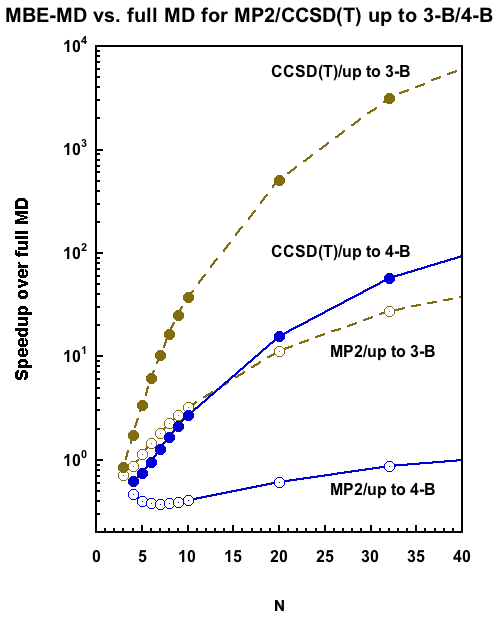
\includegraphics[width=\textwidth]{Figures/Chapter_4/ch4_figure_2.png}
\end{minipage}
\end{center}
\begin{spacing}{1.0}
\caption[Speed-up of the MBE truncated at the 3- (dotted lines) and the 4-body (solid lines) terms relative to the calculation of the full system for the MP2 (open circles) and the CCSD(T) (filled circles) electronic structure methods.]{Speed-up of the MBE truncated at the 3- (dotted lines) and the 4-body (solid lines) terms relative to the calculation of the full system for the MP2 (open circles) and the CCSD(T) (filled circles) electronic structure methods.}\label{fig:MBE_MD_F2}
\end{spacing}
\end{figure}

\par One should only expect to see gains from the MBE when the maximum order of the MBE is smaller than the polynomial scaling of the method used to compute the potential energies of each fragment. This means that for linear or even low scaling methods, the MBE will never be more efficient than just carrying out the full calculation. Figure \ref{fig:MBE_MD_F2} shows the relative speedups of the MBE truncated at the 3- (dotted lines) and the 4-body (solid lines) terms relative to the calculation of the full system for the MP2 (formal scaling as $N^5$) and the CCSD(T) (formal scaling as $N^7$) electronic structure methods. As it can be seen, the more expensive (larger scaling with $N$) the electronic structure method is, the larger the speedup for truncation to the 3- or the 4-body term. For instance, for N=10 there is a $\sim$40x speedup of the MBE truncated at the 3-body term over the full calculation at the CCSD(T) level of theory with this speedup increasing to \textgreater500x for N=20 and to \textgreater48,000x for N=64. The MBE calculation can be furthermore made more efficient by realizing that there is an optimum (different) number of processors that can be used for the parallelization of the corresponding dimer and trimer subclusters.

\par The above discussion presents the worst-case scenario for the scaling of the MBE with respect to the full calculation, yet it still looks encouraging if one wishes to use a method like CCSD(T), which scales as $O(N^7)$. The cost and scaling of the MBE can be further improved for larger systems by:
\par (i) evaluating the 3-body terms at a lower level of theory, such as HF or even using classical schemes, as previously suggested\autocite{heindel_many-body_2020},
\par (ii) developing descriptors that can be used to screen and discard or even approximate the calculation of trimers if they are, for example, too far apart. Indeed, there have been applications of both distance thresholding\autocite{cui_theoretical_2006} and energy thresholding,\cite{liu_energy-screened_2019} the latter achieving near-linear scaling in the 3-body term while introducing an overall error of less than 0.1 kJ/mol,
\par (iii) refining the thresholding schemes, a fact that can result in a more effective scaling of the 3- and 4-body terms since even the existing distance and energy thresholds would greatly improve the speedup for these higher-order terms,
\par (iv) applying machine learning or artificial intelligence approaches to discard trimers and/or tetramers and even approximate the 2-body energies based on distance thresholds.

\section{Results and Discussion}
\subsection{Averages from Classical Dynamics and Vibrational Density of States}
\par We have recently reported an exhaustive analysis of the convergence of each many-body term in the MBE for water clusters.\autocite{heindel_many-body_2020} One result from that study, which corroborates similar calculations from earlier work,\autocite{lao_understanding_2016} is that in water clusters the energy is quantitatively recovered (within about \textless2\%) by the 4-body term. The breakdown of the contribution to the binding energy is roughly 80\%, 18\%, and 2\% from the 2-, 3-, and 4-body terms, respectively. The 1-body term also makes a small repulsive contribution due to deformation of the monomers caused by the formation of the hydrogen bonds.

\begin{figure}[t]
\uwsinglespace
\begin{center}
\begin{minipage}{0.8\textwidth}
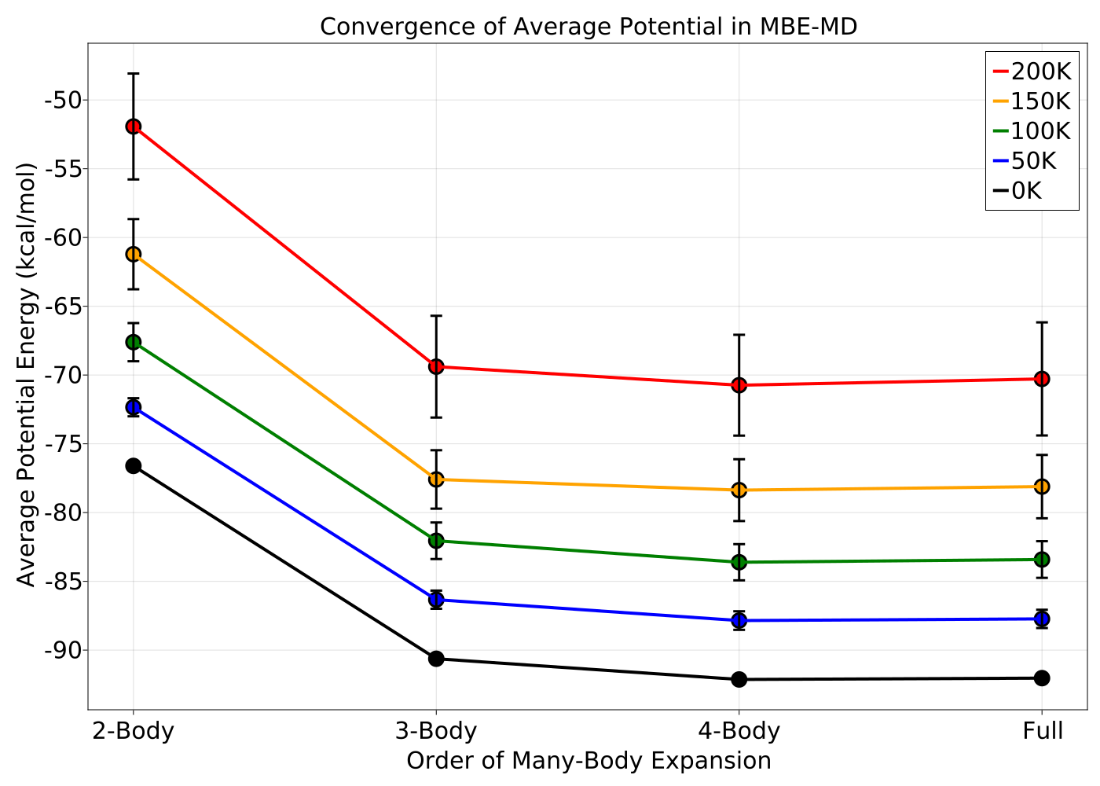
\includegraphics[width=\textwidth]{Figures/Chapter_4/ch4_figure_3.png}
\end{minipage}
\end{center}
\begin{spacing}{1.0}
\caption[Convergence of the average potential energy from MBE-MD at T=50K, 100K, 150K, and 200K when driven with a 2-, 3-, and 4-body representation of the potential. Error bars show the standard deviation of the average potential energy. Note that these do not represent uncertainties in the average energy, but the intrinsic fluctuations in potential energy due to thermal energy. The T=0K data correspond to an MBE from single point energies calculated on the minimum of the full PES.]{Convergence of the average potential energy from MBE-MD at T=50K, 100K, 150K, and 200K when driven with a 2-, 3-, and 4-body representation of the potential. Error bars show the standard deviation of the average potential energy. Note that these do not represent uncertainties in the average energy, but the intrinsic fluctuations in potential energy due to thermal energy. The T=0K data correspond to an MBE from single point energies calculated on the minimum of the full PES.}\label{fig:MBE_MD_F3}
\end{spacing}
\end{figure}

\par One obvious question, which has not been addressed before, is whether the convergence of the average potential energy during an MBE-MD simulation will follow the same pattern as for the MBE for a fixed geometry, i.e., at the minimum energy structure. Figure \ref{fig:MBE_MD_F3} shows the average potential energy taken from twelve different MBE-MD simulations. During these twelve simulations the dynamics of \ce{(H2O)_{10}} were driven by a 2-, 3-, and 4-body representation of the MB-Pol potential at temperatures of 50K, 100K, 150K, and 200K. Additionally, we ran classical MD simulations with the full potential at these temperatures. The T = 0K results correspond to an ordinary MBE for the optimized structure of \ce{(H2O)_{10}} cluster.

\par From Figure \ref{fig:MBE_MD_F3} it is seen that at the temperatures considered in this study, the average potential energy follows essentially the same convergence pattern as the convergence of the binding energy for static geometries. This finding suggests that being higher up in the potential-well does not affect the relative contributions of each term in the MBE. Interestingly, while the magnitudes of the 3- and 4-body contributions to the energy are quite similar within each temperature, their percentage of the total energy increases with temperature. Thermal energy seems to increase the 2-, 3-, and 4-body energies equally, suggesting that the percentage of the 3- and 4-body energies grows as the percentage of the 2-body energy shrinks. The non-constant percentage contribution of the many-body energy and forces may explain why pairwise additive potentials have a difficult time describing a range of temperatures and pressures. This class of potentials attempts to fold the many-body effects into an effective 2-body term, usually by using an enhanced dipole with respect to the gas phase monomer. The fact that the percentage contribution of many-body effects to the total energy is not constant with temperature means that the accuracy of this class of potentials will degrade as one moves further away from the region of the phase diagram for which they were parameterized.

\begin{figure}[t]
\uwsinglespace
\begin{center}
\begin{minipage}{0.9\textwidth}
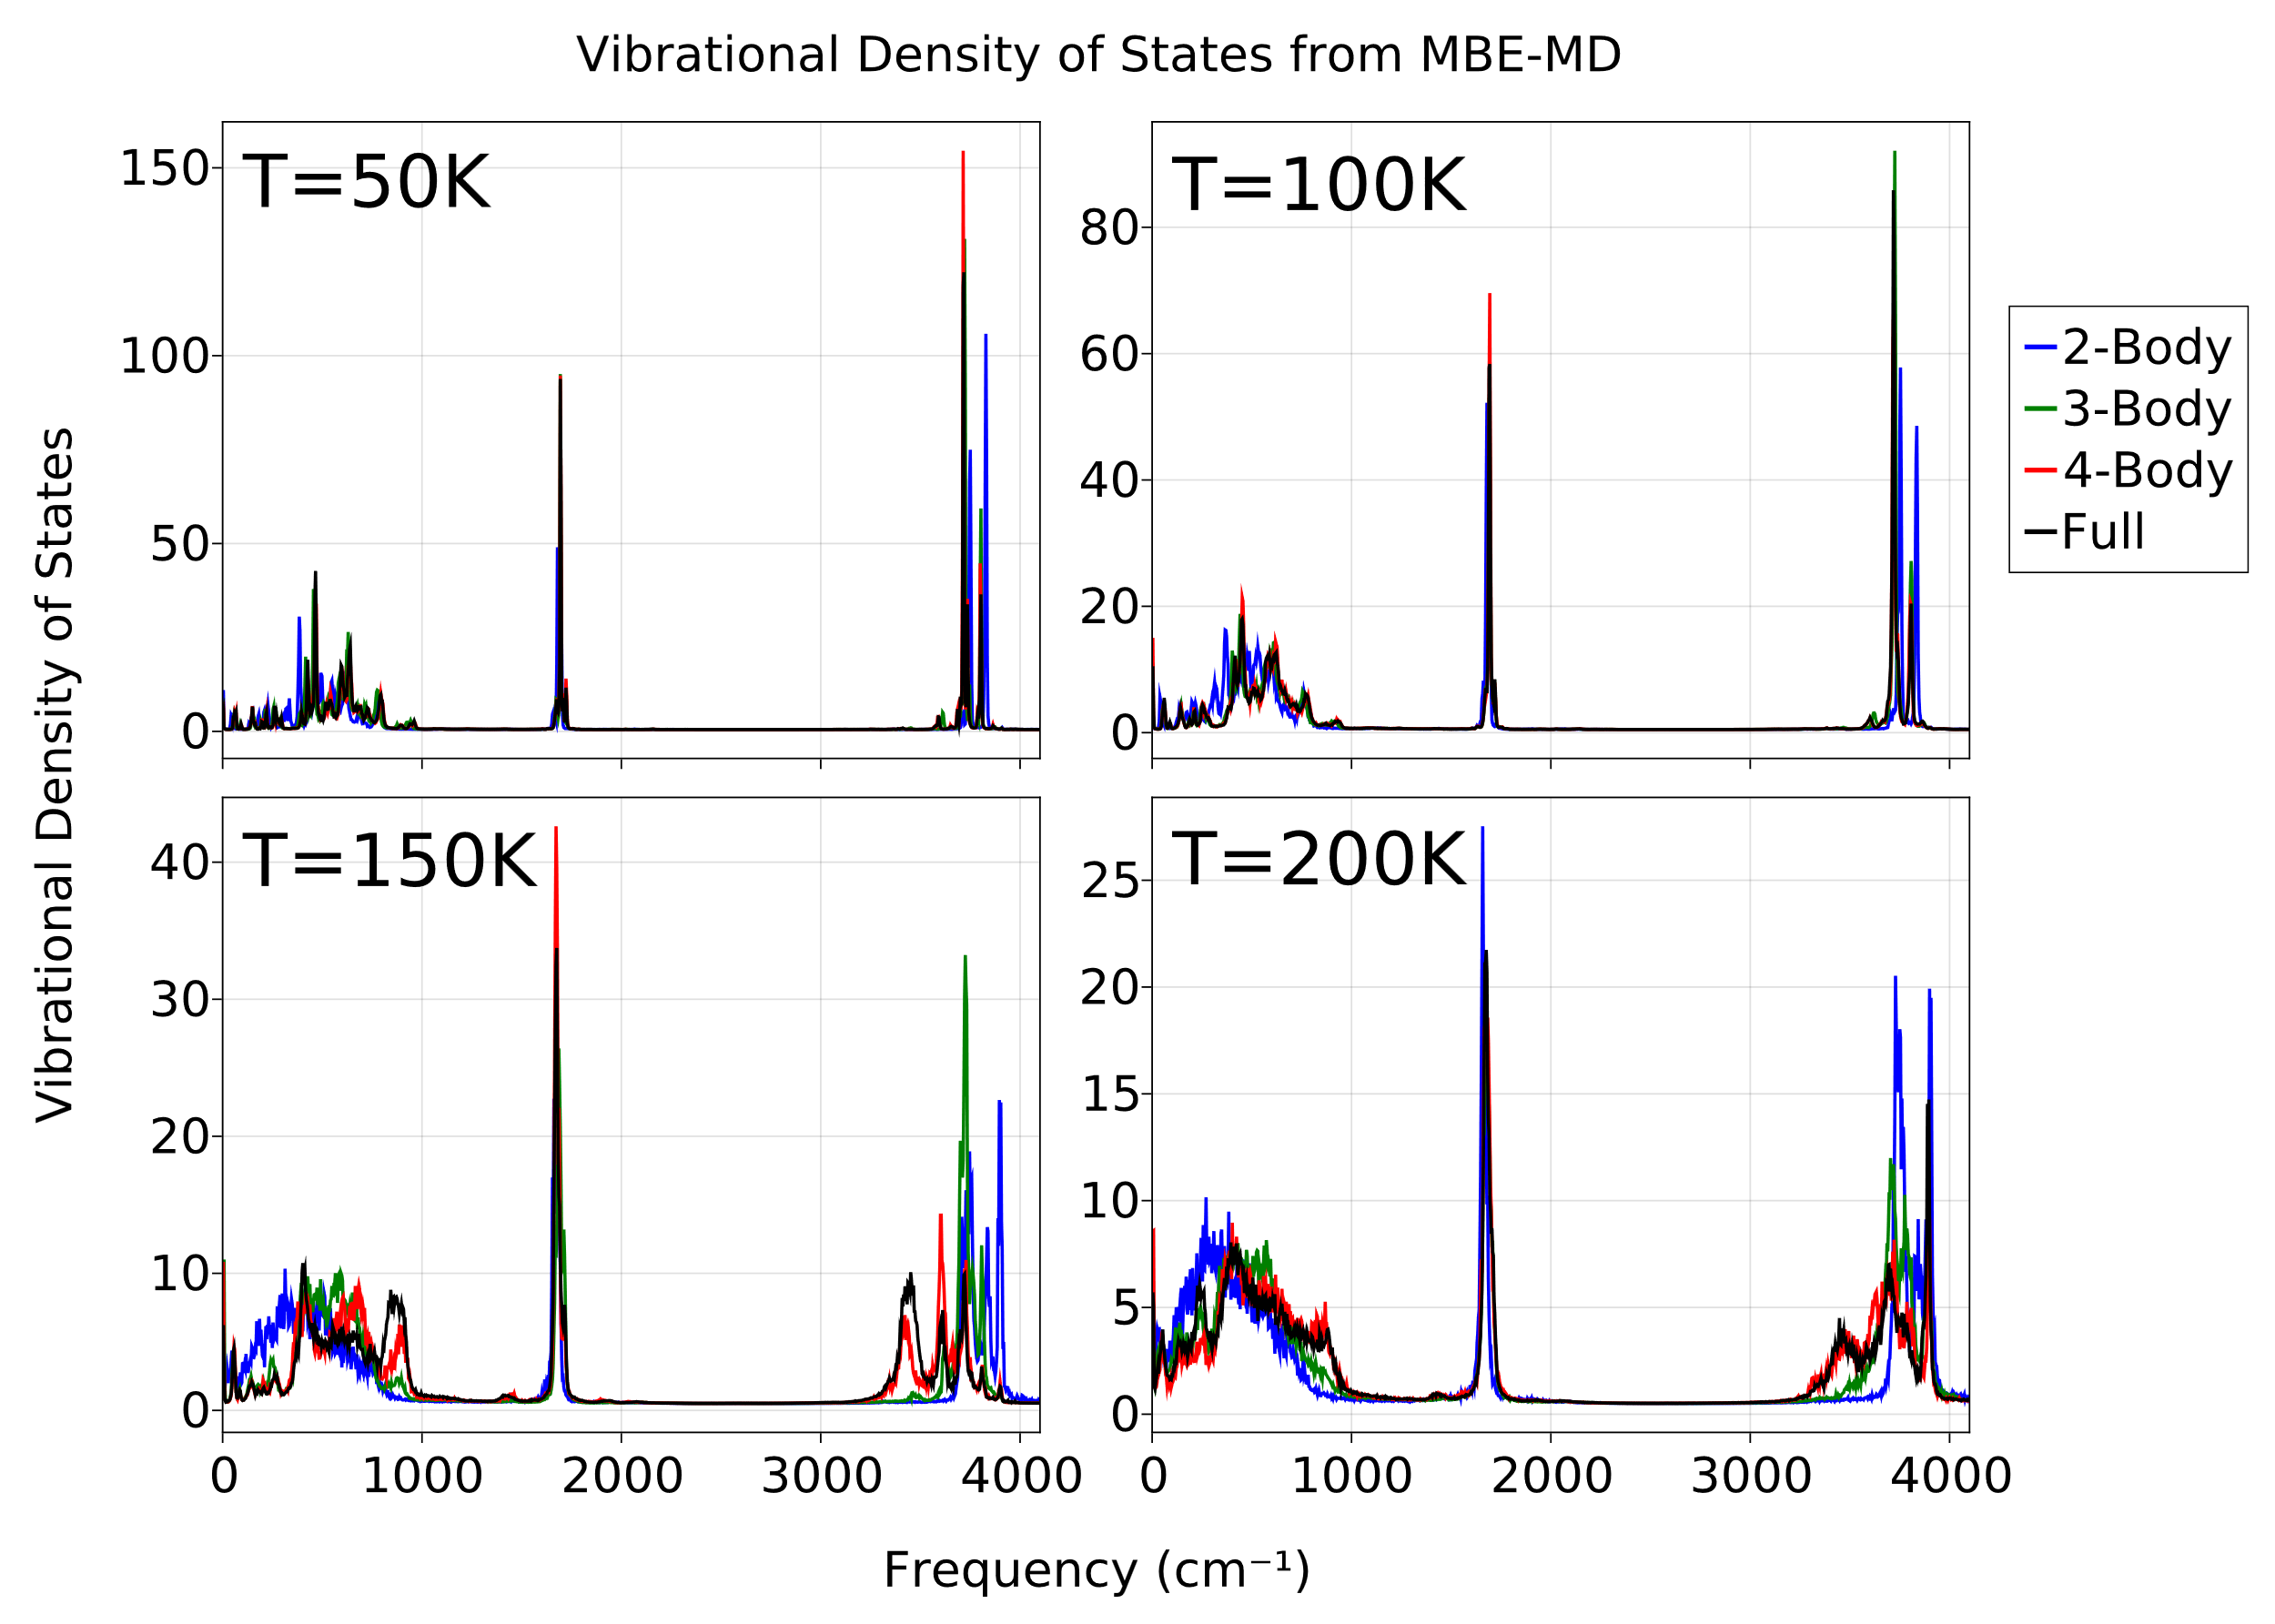
\includegraphics[width=\textwidth]{Figures/Chapter_4/ch4_figure_4.png}
\end{minipage}
\end{center}
\begin{spacing}{1.0}
\caption[Vibrational density of states as calculated from a 2-, 3-, and 4-body representation of the forces at temperatures of 50K, 100K, 150K, and 200K. The VDOS calculated from the full system is also shown for comparison. Note that each panel has a different y-axis because thermal broadening results in significantly decreased maximum intensity.]{Vibrational density of states as calculated from a 2-, 3-, and 4-body representation of the forces at temperatures of 50K, 100K, 150K, and 200K. The VDOS calculated from the full system is also shown for comparison. Note that each panel has a different y-axis because thermal broadening results in significantly decreased maximum intensity.}\label{fig:MBE_MD_F4}
\end{spacing}
\end{figure}

\par The VDOS provides a comprehensive view of the dynamics of a system and will reveal inaccuracies in the dynamics of a system over the entire fundamental frequency range. For this reason, we have calculated the VDOS with a 2-, 3-, and 4-body representation of the forces at four different temperatures. We compare the results of these MBE-MD calculations with the VDOS from calculations with the full potential in Figure \ref{fig:MBE_MD_F4}. Inferences from the results for the VDOS are quite similar to those discussed earlier for the harmonic frequencies. This is quite encouraging as the VDOS is a much better measure of the convergence of the forces than the harmonic frequencies. It should not come as a surprise that the 2- and 3-body descriptions of the dynamics are insufficient to reproduce the peak positions and intensities of the full calculations. While there are some minor discrepancies in intensities at the 4-body level, the peak positions at that level of MBE truncation (up to 4-body) are essentially the same as those for the full potential.

\begin{figure}[h]
\uwsinglespace
\begin{center}
\begin{minipage}{0.9\textwidth}
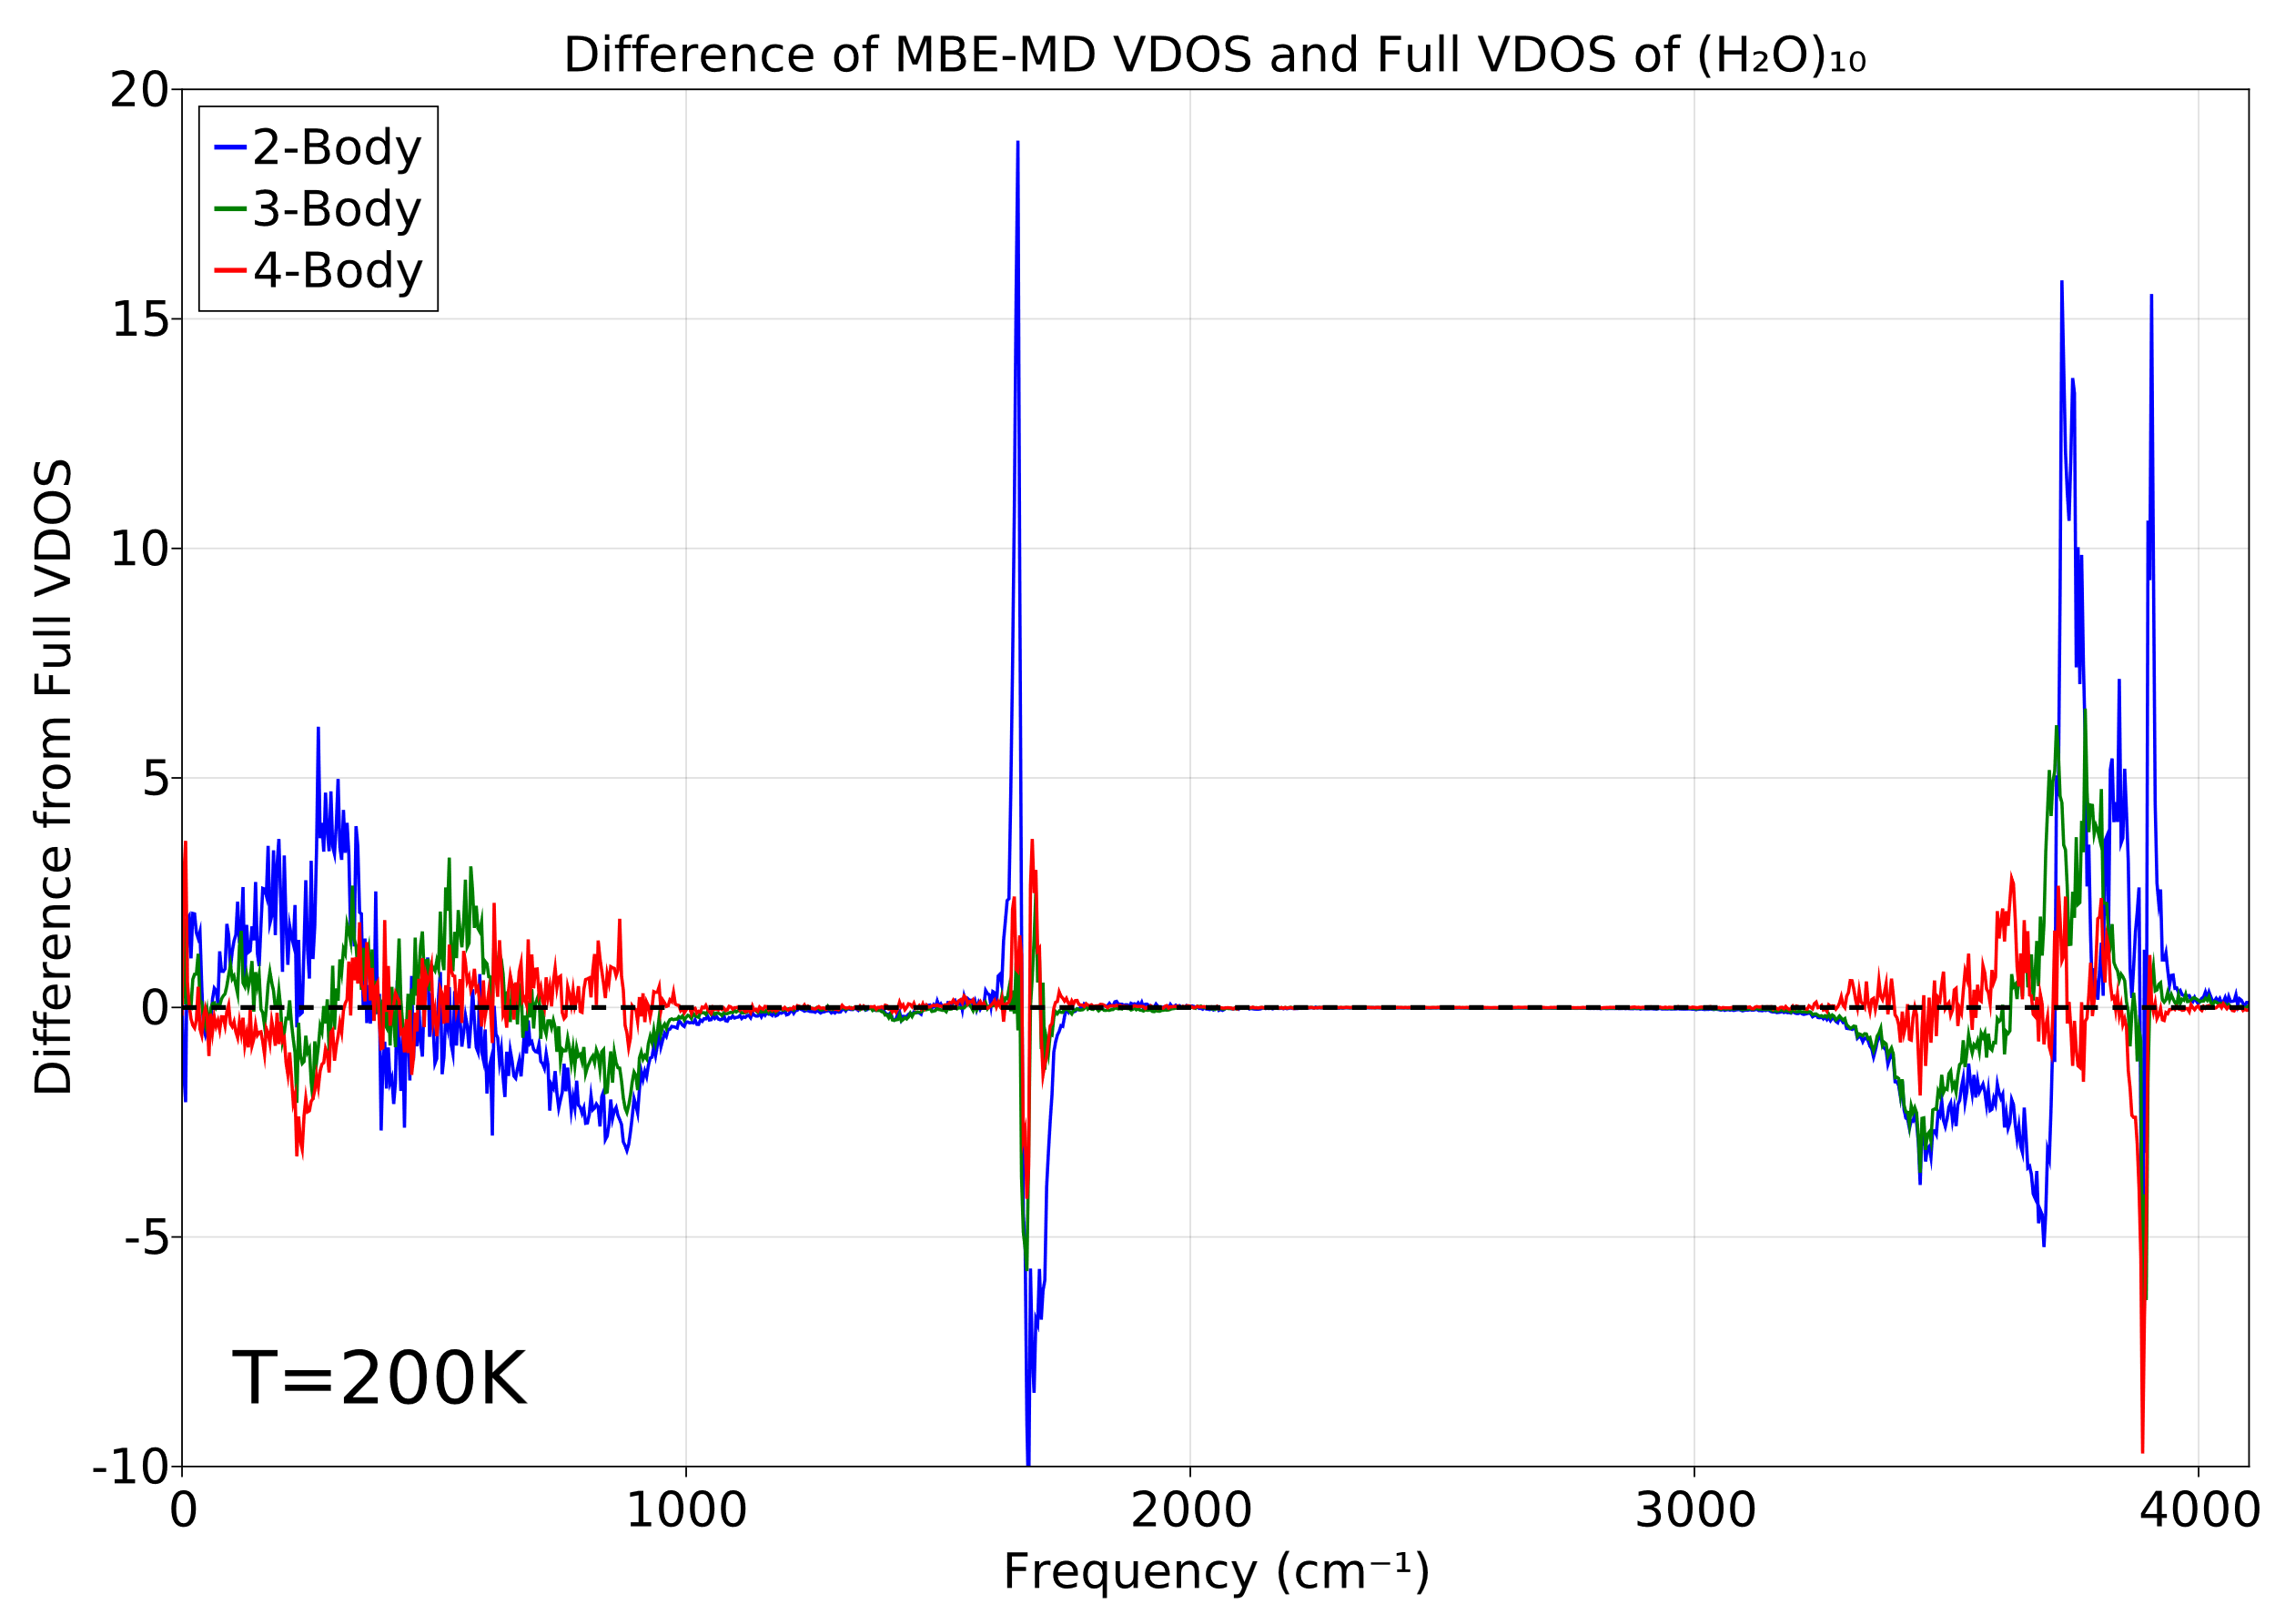
\includegraphics[width=\textwidth]{Figures/Chapter_4/ch4_figure_5.png}
\end{minipage}
\end{center}
\caption[Difference of the full vibrational density of states (VDOS) of (H2O)10 at T=200K from the VDOS calculated with a 2-, 3-, and 4-body representation of the forces.]{Difference of the full vibrational density of states (VDOS) of (H2O)10 at T=200K from the VDOS calculated with a 2-, 3-, and 4-body representation of the forces.}
\label{fig:MBE_MD_F5}
\end{figure}

\par In order to make the comparison clearer, we also show the difference of the VDOS calculated from MBE-MD from the full VDOS in Figure \ref{fig:MBE_MD_F5}. We only show the results for T = 200K as the peaks are sufficiently broad at this temperature that the difference is not skewed by tiny differences in vibrational frequencies as is the case for the T = 50K and T = 100K simulations. Essentially, at T = 200K the VDOS is converged at the 4-body level. This is a very stringent test of the convergence of the forces and further strengthens the usefulness of the MBE-MD protocol in future studies.

\par An important point about the MBE, which has not been fully appreciated in the past, is that it is completely composable. That is, there is no reason at all that one needs to use the same level of theory, or even use an ab initio method, at all orders of the MBE. Different levels of theory, whether these are quantum electronic structure, classical molecular mechanics or even electrostatic models can be stitched together to provide the individual components that make up the MBE. Indeed, we have recently shown that the 3-body term of the MBE can be sufficiently described (to high accuracy) at the Hartree-Fock (HF) level of theory.\autocite{heindel_many-body_2020} This realization paves the way for a highly accurate AIMD scheme in which the 1- and 2-body energies and forces can be evaluated at a level as high as CCSD(T) and the 3-body and higher orders are layered on at the HF level. Because the correlation contribution to the energy is negligible beyond the 2-body, this composite scheme should yield dynamics of near CCSD(T) level accuracy. Finally, note that one need not even calculate all parts of the same MBE rank at the same level of theory. Indeed, one could pre-select certain important dimers to evaluate at a higher level of electronic structure theory, i.e., CCSD(T), and calculate the rest of the dimers at a lower level of theory or even a classical representation. Albeit this is not exact, it would lead to a tremendous speed up in calculation time and should allow for accuracies at least on par with commonly used QM/MM techniques. Additionally, mixing classical and quantum methods is much more straightforward within MBE-MD than in QM/MM because the sub-systems are naturally separated so that no couplings between the sub-systems needs to be considered. This contrasts with QM/MM where coupling the classical and quantum regions introduces significant complexity in the calculations.\autocite{liu_qmmm_2014,laino_efficient_2005,laino_efficient_2006,loco_towards_2019} Note that MBE-MD and QM/MM are compatible with each other so one could choose to describe the QM region of a QM/MM calculation via an MBE. These connections represent an exciting research path which we are planning to pursue in the near future.

\subsection{Forces}

\par While energies are important for the description of thermodynamic quantities, the forces are far more important for molecular dynamics. Demerdash and Head-Gordon have suggested that the forces in polarizable potentials may only converge by the 5-body term in the MBE.\autocite{demerdash_assessing_2017} This is in contrast to nearly every other molecular quantity, which are practically converged at the 4-body if not by an earlier term,\autocite{bates_development_2011,medders_many-body_2013,xantheas_cooperativity_2000} with the exception of highly anharmonic vibrations.\autocite{heindel_origin_2018} In order to study the convergence of the forces, we treat the forces on the system as one 3N-dimensional vector (where N is the number of atoms). We then compare the length of this vector with the length of the full forces as well as the angle between these vectors. To make this comparison, we take an uncorrelated sample of 4590 structures from an MD simulation at T = 200K with the MB-Pol potential and compute the MBE of the forces up to the 7-body term for each structure.

\begin{figure}[h]
\uwsinglespace
\begin{center}
\begin{minipage}{0.45\textwidth}
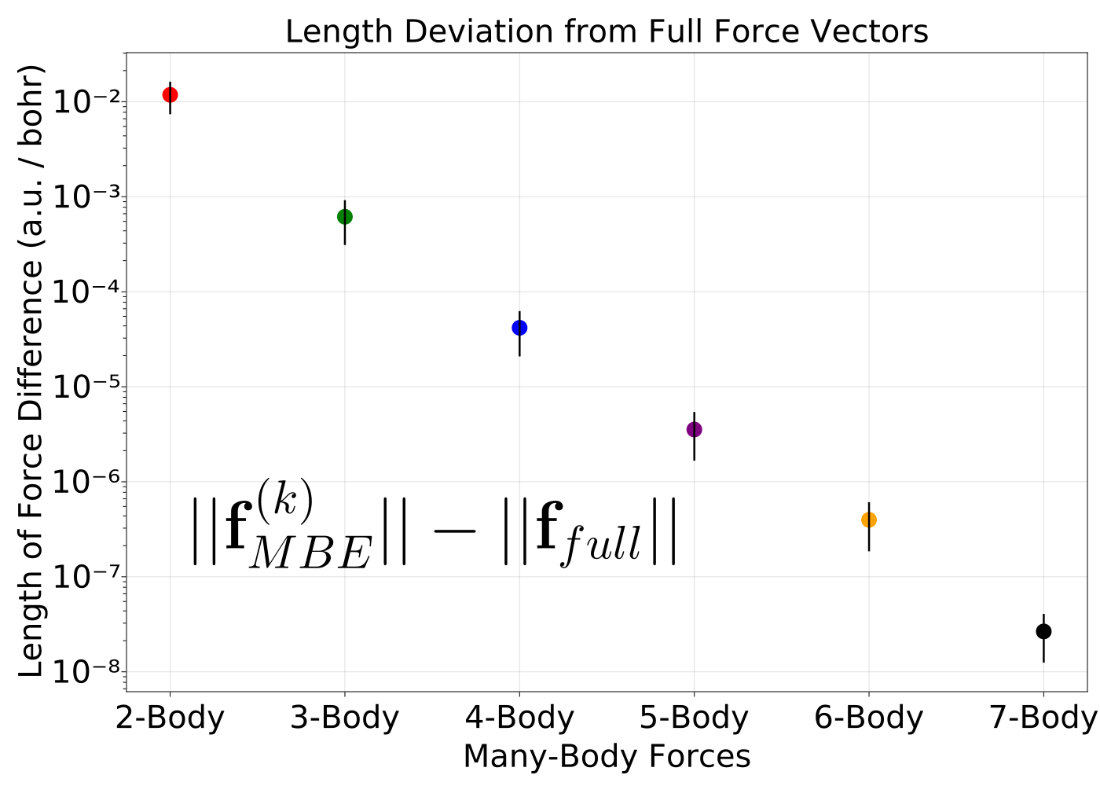
\includegraphics[width=\textwidth]{Figures/Chapter_4/ch4_figure_6_top.png}
\end{minipage}
\begin{minipage}{0.45\textwidth}
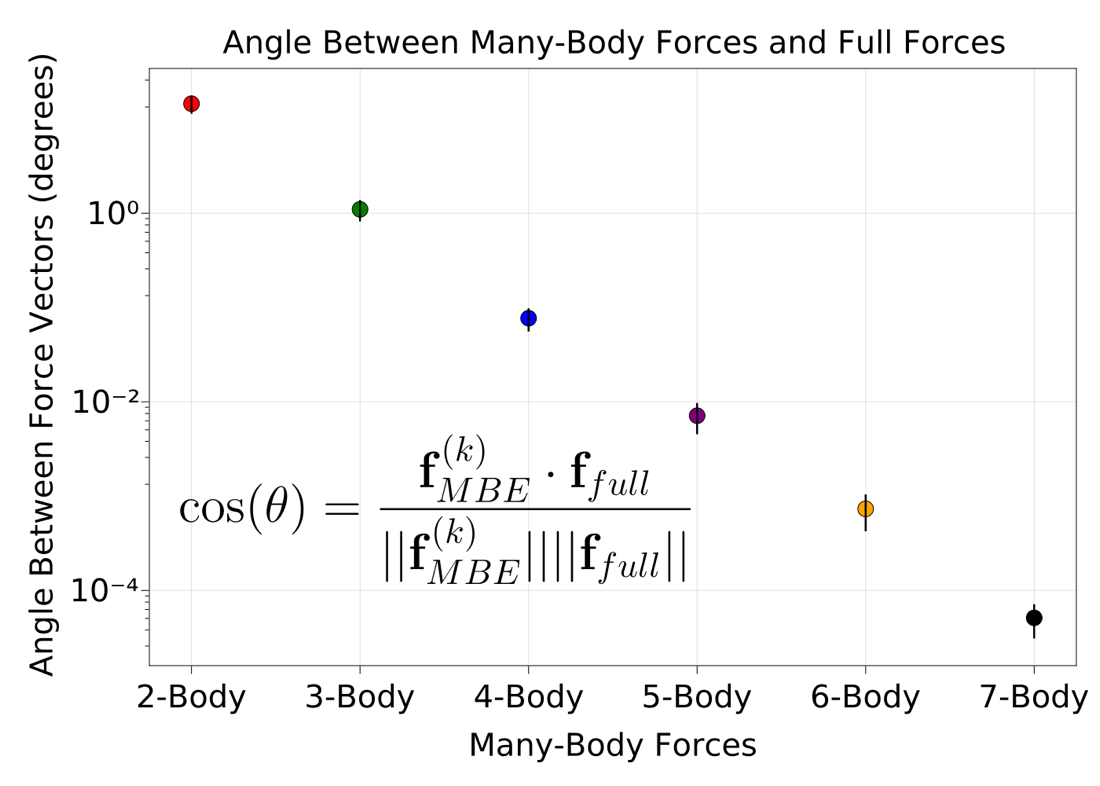
\includegraphics[width=\textwidth]{Figures/Chapter_4/ch4_figure_6_bottom.png}
\end{minipage}
\end{center}
\caption[(Convergence of the length difference between MBE forces and full forces $||f^{(k)}_{MBE}||-||f_{full}||$ where the MBE forces are calculated up to order . (6b, right) Convergence of the angle between $f^{(k)}_{MBE}$ and $f_{full}$.]{(left) Convergence of the length difference between MBE forces and full forces $||f^{(k)}_{MBE}||-||f_{full}||$ where the MBE forces are calculated up to order . (right) Convergence of the angle between $f^{(k)}_{MBE}$ and $f_{full}$. Notice the log-scale in these plots which makes the error bars appear to be asymmetric when the fluctuations are, in fact, normally distributed around each point.}
\label{fig:MBE_MD_F6}
\end{figure}

\par Figure \ref{fig:MBE_MD_F6} shows the difference in length of the MBE forces calculated up to the $k$-body term from the full forces, $||f^{(k)}_{MBE}||-||f_{full}||$. The average difference between the magnitude of the 4-body forces and full forces is $-1.11\cdot 10^{-5}$ a.u./bohr, while the median force magnitude for this system is $0.222$ a.u./bohr, meaning the force magnitudes are converged to about $5\cdot 10^{-5}$ a.u./bohr. The lengths of the forces are converged to within $10^{-3}$ a.u./bohr even at the 3-body level.

\par The angle between the force vectors seems to asymptotically converge to zero deviation with each order of the MBE improving the angle deviation by about one order of magnitude. Figure \ref{fig:MBE_MD_F6} shows that at the 4-body level, the angle between $f^{(4)}_{MBE}$ and $f_{full}$ is converged to about 0.01 degrees. This amount of angle deviation is apparently sufficient that the average potential energy and vibrational density of states are converged by the 4-body term. Nonetheless, this convergence pattern is quite unusual compared to e.g., the convergence of the energy as described by the MBE.

\par This slower convergence of the angle between the MBE(k) and full forces essentially places a bound on how tightly one can converge a geometry relative to a reference or match the dynamics of a full system. For instance, at the 4-body level, the root-mean-squared deviation (RMSD) averaged over all 4590 \ce{(H2O)_{10}} structures is converged to $3.15\cdot 10^{-5}$ a.u./bohr, while at the 5-body level the RMSD is $2.91\cdot 10^{-6}$ a.u./bohr. Depending on the calculation of interest, this may or may not be a sufficient level of convergence. For the case of molecular dynamics, we have not seen evidence that the average energy or VDOS are noticeably affected by this deviation in the forces.

\par The slower convergence of forces also highlights the importance for many-body potentials to include an approximate electrostatic scheme on top of the explicitly fitted many-body terms. For instance, MB-Pol contains explicit 1-, 2-, and 3-body terms, but includes all orders of the MBE by layering on electrostatics as calculated by the TTM4-F model.\autocite{burnham_vibrational_2008} Our results suggest that without the addition of these higher-order terms it would be difficult to simultaneously match the forces and energies to reference calculations.

\par We should emphasize that it is not all that surprising to see an asymptotic convergence towards the full-MBE limit. The surprising result is that even at the 5-body level the deviation from the full forces is non-negligible. For instance, the MBE of the energy up to 4-body is usually converged to around 0.1-0.01 kcal/mol. This is well within so-called chemical accuracy (1 kcal/mol) and hence is not considered problematic. On the other hand, it is not uncommon to converge forces to $10^{-5}$ a.u./bohr when using tight thresholds on a geometry optimization. 

\subsection{Harmonic Frequencies}

\par Oftentimes, harmonic frequencies offer a simple picture of the dynamics of a system near a local minimum on the PES. In Figure \ref{fig:MBE_MD_F7}, we show the deviation of the harmonic frequencies calculated with a 2-, 3-, and 4-body representation of the MB-Pol potential from the corresponding harmonic frequencies calculated with the full potential. Since each of these $k$-body representations of the PES will have a slightly different local minimum structure of the chosen isomer of \ce{(H2O)_{10}}, we re-optimized the cluster on each of the $k$-body PESs and performed a harmonic analysis with the same representation of the PES.

\begin{figure}[t]
\uwsinglespace
\begin{center}
\begin{minipage}{0.8\textwidth}
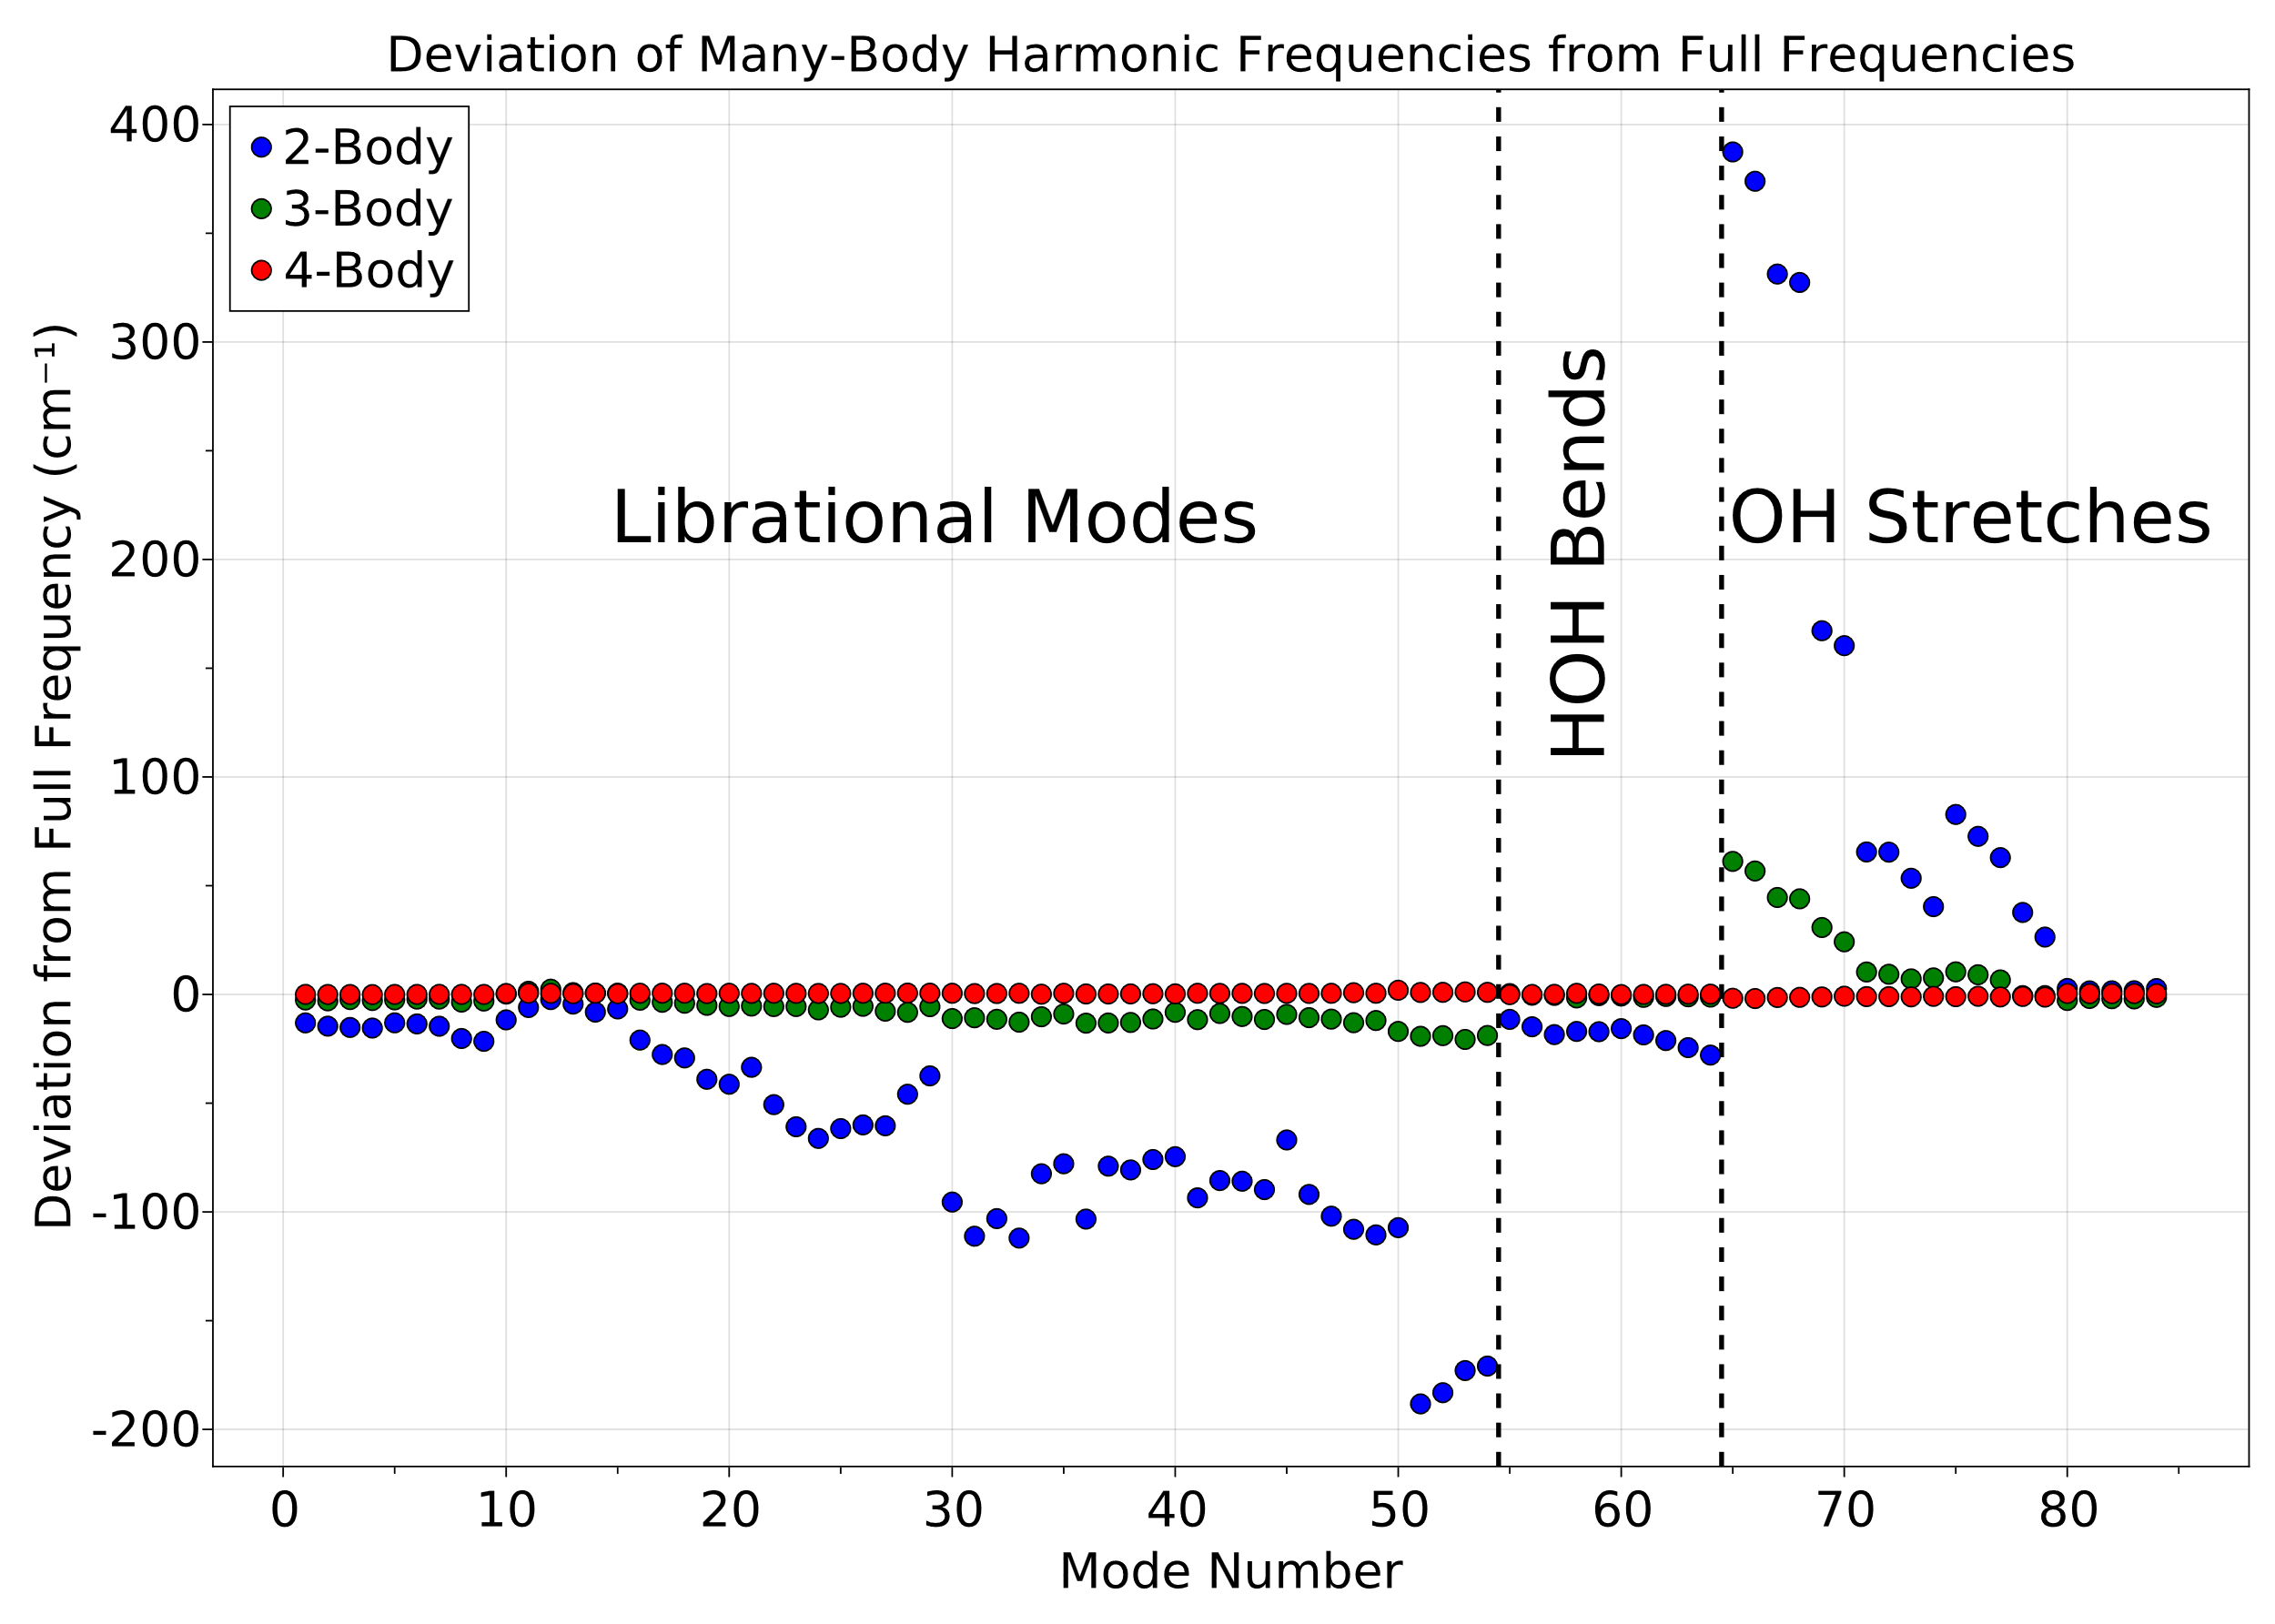
\includegraphics[width=\textwidth]{Figures/Chapter_4/ch4_figure_7.png}
\end{minipage}
\end{center}
\begin{spacing}{1.0}
\caption[Deviation of harmonic frequencies at 2-, 3-, and 4-body levels using the MB-Pol potential. The \ce{(H2O)_{10}} cluster of interest was re-optimized using the MBE and harmonic frequencies were calculated at each minimum using the $k$-body potential.]{Deviation of harmonic frequencies at 2-, 3-, and 4-body levels using the MB-Pol potential. The \ce{(H2O)_{10}} cluster of interest was re-optimized using the MBE and harmonic frequencies were calculated at each minimum using the $k$-body potential. The x-axis simply labels the mode number starting from the lowest frequency harmonic vibration and the y-axis shows deviation from the full harmonic frequencies. The dashed lines separate low-frequency librational modes from HOH bends and OH stretches. The 4-body representation has a maximum deviation of less than 5 $\mathrm{cm}^{-1}$ in the OH stretches.}\label{fig:MBE_MD_F7}
\end{spacing}
\end{figure}

\par Some interesting trends are clear from this harmonic picture. Clearly, both 2- and 3-body representations of the PES are woefully deficient, showing deviations in the hydrogen-bonded OH stretches of up to about 375 $\mathrm{cm}^{-1}$ (for the 2-body) and 75 $\mathrm{cm}^{-1}$ (for the 3-body), respectively. Therefore, as with the potential energy, at least a 4-body representation of the PES is required to quantitatively capture the vibrational frequencies for this system. Additionally, all low-frequency vibrations, which are more important than OH stretches for the long-time dynamics, are blue-shifted relative to the frequencies obtained with the full PES. The HOH bends seem to converge faster than OH stretches and librations, while being blue-shifted relative to the frequencies on the full PES.

\par The inaccurate red-shifts of the OH stretches with just the 2-body term indicate that a many-body PES is required to adequately describe cooperative hydrogen-bonding in water clusters. This is somewhat tautological, as the definition of hydrogen bond cooperativity is the presence of large many-body contributions to the binding energy, but nonetheless confirms what one would suspect in the context of vibrational frequency shifts rather than binding energies. These frequency deviations seem to reveal an underappreciated trend, which is that many-body effects seem to stiffen the low-frequency dynamics relative to a strictly pairwise additive potential. One interpretation of this is that hydrogen-bond cooperativity strengthens the coupling between OH stretches and various low-frequency motions, such as the OO stretch, which has been observed, for example, in protonated water cluster systems.\autocite{duong_tag-free_2018}

\subsection{Extension to nuclear statistical mechanical path integral MD simulations}

\par In the interest of completeness of the proposed MBE-MD protocol, we have also considered the extension of the classical MBE-MD to incorporate nuclear statistical mechanical degrees of freedom via path integral molecular dynamics (PIMD),\autocite{chandler_exploiting_1981,feynman_quantum_2010} which we abbreviate as MBE-PIMD. This extension is straightforward, since the evaluation of the potential is not different between PIMD and ordinary MD. The application of the MBE-PIMD for the ring water tetramer, \ce{(H2O)4}, is shown in Figure \ref{fig:MBE_MD_F8}. We use a time step of 0.25 fs to integrate the equations of motion on the TTM2.1-F potential energy surface. The simulations are thermostatted using the PIGLET colored-noise thermostat\autocite{ceriotti_efficient_2012}, which allows for well-converged energies using 64 beads. Each simulation is carried out for 600 ps.

\begin{figure}[t]
\uwsinglespace
\begin{center}
\begin{minipage}{0.8\textwidth}
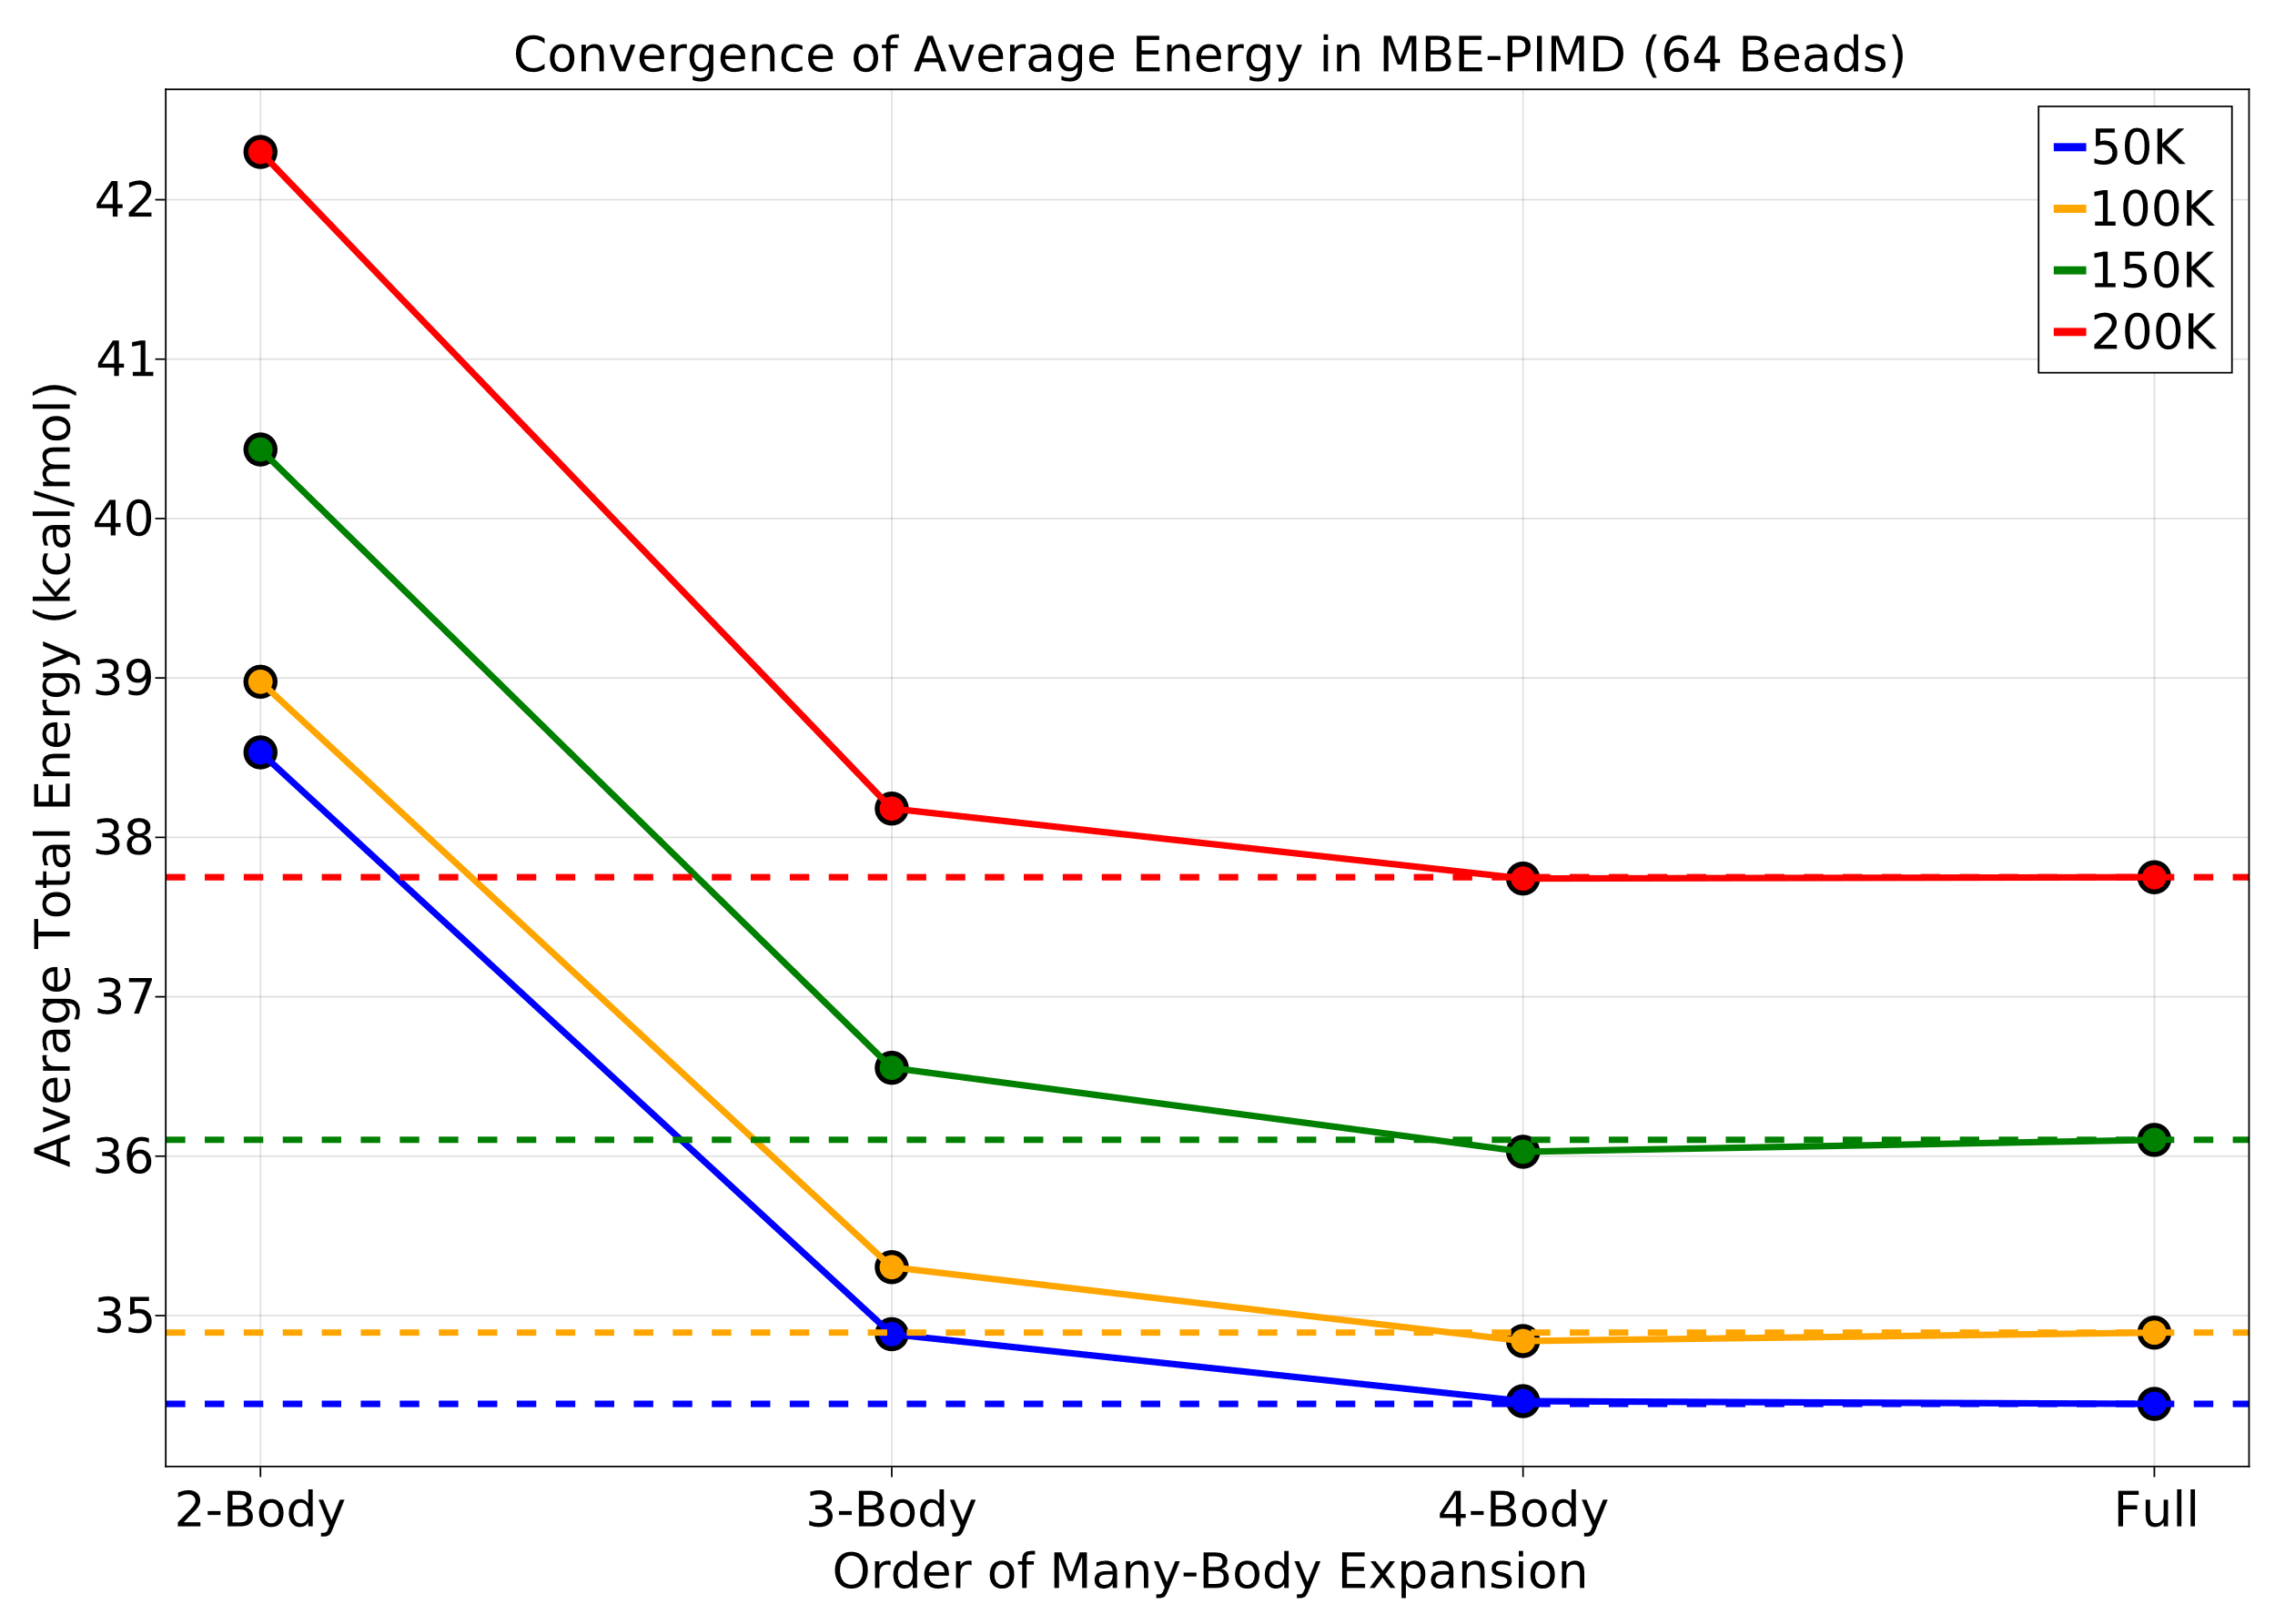
\includegraphics[width=\textwidth]{Figures/Chapter_4/ch4_figure_8.png}
\end{minipage}
\end{center}
\begin{spacing}{1.0}
\caption[Convergence of MBE-PIMD with temperature, using 64 beads for each ring polymer, for \ce{(H2O)4} calculated with a 2-, 3-, and 4-body representation of the forces.]{Convergence of MBE-PIMD with temperature, using 64 beads for each ring polymer, for \ce{(H2O)4} calculated with a 2-, 3-, and 4-body representation of the forces.}\label{fig:MBE_MD_F8}
\end{spacing}
\end{figure}

\par The results in Figure \ref{fig:MBE_MD_F8} demonstrate the convergence of MBE-PIMD to the full PIMD simulation for \ce{(H2O)4}. Because this cluster only contains four monomers, the full PIMD simulation and the simulation driven by 4-body forces should be identical to within statistical accuracy, as they are. Ordinarily, 32 beads is taken to be the largest number of beads necessary to converge PIMD simulations for liquid water.\autocite{ceriotti_i-pi_2014} In this case, the energy seems to be converged to within a few tenths of 1 kcal/mol. Depending on the accuracy one is trying to achieve, this may or may not be acceptable. For instance, if one is interested in extrapolating to the zero temperature limit to estimate zero-point energy, or otherwise interested in very low-temperature simulations,\autocite{uhl_accelerated_2016,schran_quantum_2019} then 64 beads is likely insufficient for clusters. Presumably, this is because of the virtual absence of free OHs in the bulk of liquid water, whereas free OH bonds are quite common in water clusters, allowing for greater proton delocalization.

\section{Conclusions}

\par The MBE(k)-MD protocol, where $k$ is the maximum order of the MBE, formally scales as $O(N^k)$. This means that the MBE is only asymptotically advantageous when using an electronic structure method which scales as a polynomial greater than $O(N^k)$. Truncation at the 3- and/or 4-body term, which is adequate to produce converged energies and forces for water, results in substantial savings over the full calculation for methods including higher levels of electron correlation, such as CCSD(T). In contrast, no savings are realized for using DFT or lower scaling methods as the underlying electronic structure to evaluate the sub fragment clusters. The MBE-MD scheme is trivially parallelizable and can further explore second level parallelization of the underlying electronic structure method used to evaluate the various sub fragments.

\par We have reported the convergence properties of MBE-MD simulations at various orders of the MBE using classical water potentials to evaluate the harmonic frequencies and vibrational density of states of the \ce{(H2O)_{10}} cluster. Our results indicate that the convergence of forces and the average energy during an MBE-MD simulation follows essentially the same trend as has been previously reported for the water cluster minima. The 4-body term is necessary to achieve quantitative accuracy, however truncation up to the 3-body was found to provide near-quantitative results compared with the full (not truncated) PES. This is an encouraging first foray into the new MBE-MD protocol as it means much of the accumulated knowledge about convergence properties and accuracy of the ordinary MBE can transfer to the molecular dynamics context.

\par The extension of the classical to the nuclear statistical description of the nuclei is straightforward; we have demonstrated this by reporting the first MBE-PIMD simulations for the ring \ce{(H2O)4} cluster. PIMD and MBE-MD have a great synergy since all sub-system calculations required for the MBE and that of the beads required for the PIMD are completely separable. It would be feasible to achieve near perfect parallelism of all the numerous sub-system calculations required by this protocol for both the MBE-MD and MBE-PIMD simulations. It seems likely that a better integration of GPU-based electronic structure and MD will greatly aid in the future of this effort.

\par In our opinion, the flexibility and simplicity of the MBE will allow for future MD simulations at unprecedented levels of accuracy. Namely, we expect that CCSD(T)-quality dynamics could be achievable by composing the appropriate methods at each order of the MBE and taking advantage of current and future developments on Leadership Computing Facilities. For systems where fragments are naturally defined, such as in clusters, liquids, and solids of hydrogen bonded molecules, the MBE-MD protocol is a very promising approach. In the near future we plan to carry out MP2- and CCSD(T)-quality MBE-MD simulations to further demonstrate the usefulness of this technique.

\chapter{Conclusions and Future Directions}

\par It is undeniable that molecular simulation is one of the most important tools available for understanding chemical systems, particularly when used in tandem with experiments. One of the biggest limitations of MD simulations comes from the trade-off between accuracy of forces and the time scale over which a simulation can be run. That is, longer time scale phenomena almost always have to be studied with less accurate or less general descriptions of the molecular interactions.

\par We have leveraged the many-body expansion to partially alleviate the trade-off between accuracy and accessible time scale in MD. We have done this by noting that the scaling of the MBE allows high-level electronic structure methods, such as MP2 and CCSD(T), to be used without paying the high scaling of the method itself because the many sub-systems in the MBE are essentially constant in size compared to the total system. Furthermore, we have shown that one only needs to calculate up to the 4-body term in the worst case to converge both energies and gradients.

\par Our detailed calculations of the MBE for water clusters showed that electron correlation is not important for the 3- and 4-body terms of the MBE as long as the BSSE correction is used. This is very important because being able to use HF or DFT for the 3-body term makes these calculations computationally feasible. The biggest problem, however, is that the cost of a BSSE correction scales with system size. For this reason, we have shown that the BSSE can be approximated by a simple function to scaled internuclear distances. While this approximation to BSSE will be useful in benchmark single-point calculations, it has limited utility for MD simulations, since MD only requires the energy gradient and not the energy itself. For this reason, further work on how to approximately correct energy gradients for BSSE needs to be explored. It is worth noting that the problem of BSSE corrections in an MD simulation goes far beyond the MBE-MD technique discussed in this thesis. That is, any \textit{ab initio} MD (AIMD) simulations using gaussian basis functions suffers from BSSE. The computationally expensive AIMD simulations performed with small basis sets will suffer from a large BSSE.

\par Even though using HF for 3- and 4-body terms represents a huge computational win over correlated methods, HF is still far more expensive than classical force fields or semi-empirical methods. For this reason, we have explored the use of advanced force fields in place of \textit{ab initio} methods for the 3- and 4-body terms. This makes the scaling of the MBE effectively $O(N^2)$ with respect to the number of fragments since advanced force fields are often three to six orders of magnitude faster than electronic structure methods. Not only that, but many advanced force fields formally scale as $O(N^2)$, so one can perform a calculation for the entire system, then subtract out the 1- and 2-body terms calculated with that force field to get the 3- through $N$-body terms all at once. This approach of layering a force field onto an \textit{ab initio} reference only involves calculations that scale as $O(N^2)$, meaning that the formal scaling of this MBE-MD scheme is independent of the scaling of the electronic structure method being used (for a fixed basi set). Future work will aim to show that this scheme can be essentially as accurate as the full AIMD calculations for water and ion-water clusters.

\par This thesis provides evidence that the many-body expansion can bridge the paradigms of molecular mechanics and \textit{ab initio} molecular dynamics. Whether or not MBE-MD, as we have described it, will achieve the promise it seems to hold depends largely on building tools to make MBE-MD simulations routine and easy, even for non-experts. This is because the main advantage of MBE-MD is that each term is totally independent of one another. This means that massively parallel computing systems (both CPUs and GPUs) must be effectively utilized. Furthermore, because each term is independent, one can combine many different types of theories. In this sense, the MBE is a recipe for creating hybrid descriptions of molecular properties. Therefore, we believe that this thesis provides the necessary validation of MBE-MD as a viable and accurate approach to molecular simulation. Therefore, the most important future work is creating effective tools, in the form of software, for efficiently computing the MBE while allowing users to control how each term is calculated, at the software level, in a hardware independent manner.

\printbibliography

\end{document}
